\documentclass[bibliography=totocnumbered]{scrartcl}

\usepackage{packages/common_packages}
\usepackage{packages/macros}
\usepackage{packages/theorem_styles}
\usepackage{packages/list_structures}
\usepackage{packages/toc}

\usepackage{tikz}

% TikZ libraries
\usetikzlibrary{babel} % https://github.com/astoff/tikz-cd/issues/7
\usetikzlibrary{cd}

% Bibliography
\addbibresource{bib/books.bib}
\addbibresource{bib/articles.bib}
\addbibresource{bib/nlab.bib}
\addbibresource{bib/proofwiki.bib}

% Document
\title{Notebook}
\subtitle{\URL{https://github.com/v--/notebook}}
\author{Ianis Vasilev, \Email{ianis@ivasilev.net}}
\date{}

\begin{document}

\hfuzz=3pt
\maketitle

\begin{abstract}
  This ever-expanding document started as a set of study notes and exercises and gradually outgrew itself to become a slightly more encyclopedic set of study notes. Having all these notes in one place is quite helpful for both expressing my own thoughts clearly and for later reference. It is also helpful for tracking connections between seemingly unrelated concepts.

  Since these are study notes, they will naturally have a lot of errors, so read them with caution. Feel free to contact me if something in this document happens to distress you.

  I tried putting citations on everything. If there is no citation on a definition or theorem, that means that I have probably recalled it from memory. The simple proofs are mostly original and the difficult ones are, often loosely, based on proofs from the places cited. The omitted proofs are either too trivial or too involved for me to spend time on them.
\end{abstract}

\newpage
\tableofcontents
\newpage

\section{Analysis}\label{sec:analysis}
\section{Analysis}\label{sec:analysis}
\subsection{Geometry of vector spaces}\label{subsec:geometry_of_vector_spaces}

\begin{definition}\label{def:real_linear_combinations}
  Let \( X \) be a real vector space\Tinyref{remark:real_vector_space} and let \( t_1, \ldots, t_n \in \BB{R} \) and \( x_1, \ldots, x_n \in X \). We say that their linear combination\Tinyref{def:linear_combination} \( x \coloneqq \sum_{k=1}^n t_k x_k \) is

  \begin{defenum}
    \DItem{def:real_linear_combinations/affine} an \textbf{affine combination} if \( \sum_{k=1}^n t_k = 1 \).
    \DItem{def:real_linear_combinations/conic} a \textbf{conic combination} if all of the coefficients are nonnegative.
    \DItem{def:real_linear_combinations/convex} a \textbf{convex combination} if it is both affine and conic. A convex combination of two elements \( x, y \in X \) is usually written as \( tx + (1-t)y \) for some scalar \( t \in [0, 1] \).
  \end{defenum}
\end{definition}

\begin{definition}\label{def:linear_combination_hulls}
  Let \( A \) be a subset of the real vector space \( X \). We define the \textbf{convex hull} \( \Conv A \) (resp. \textbf{affine hull} or \textbf{conic hull}) of \( A \) by the set of all convex (resp. affine or conic) combinations of finite subsets of \( A \).

  The convex hull \( \Conv A \) of two elements \( x, y \in X \) is often called the \textbf{segment between \( x \) and \( y \)} and is denoted as
  \begin{equation*}
    [x, y] \coloneqq \{ tx + (1-t)y \colon t \in [0, 1] \}.
  \end{equation*}

  If the set \( A \) is equal to its convex (resp. affine or conic) hull, we say that it is a \textbf{convex set} (resp. \textbf{affine set} or \textbf{cone})
\end{definition}

\begin{definition}\label{def:simplex}
  Let \( v_1, \ldots, v_n \) be linearly independent vectors and \( v_0 \) be any other vector. The convex hull \( S \) of the vectors \( v_0 + v_1, \ldots, v_0 + v_n \) is called an \textbf{n-simplex}.

  The convex hull of any nonempty subset of \( \{ v_0, \ldots, v_n \} \) of cardinality \( m + 1 \) is an \( m \)-simplex and is called an \textbf{\( m \)-face of \( S \)}.
\end{definition}

\subsection{Topological vector spaces}\label{subsec:topological_vector_spaces}

\begin{definition}\label{def:topological_vector_space}
  Let \( X \) be any vector space and let \( \CT \) be a topology on \( X \). The space \( (X, +, \cdot, \CT) \) is called a \Def{topological vector space} if the linear and topological structure agree, that is, the operations \( +: X \times X \to X \) and \( \cdot: X \times \BR \to X \) are continuous with respect to \( \CT \).

  Both the additive group \( (X, +) \) and the multiplicative group \( (X \setminus \{ 0 \}, \cdot) \) are topological groups\Tinyref{def:topological_group}. We regard \( X \) as a subgroup of its additive topological group.

  See \fullref{remark:hausdorff_topological_groups}, \fullref{def:continuous_dual_space} and \fullref{def:category_of_topological_vector_spaces} for more nuances.
\end{definition}

Given that a topological vector space \( X \) has both a topological and an algebraic structure, we should adapt certain definitions.

\begin{definition}\label{def:continuous_dual_space}
  We define the \Def{continuous dual space} \( X^* \) of a topological space \( X \) as the vector space of all continuous\Tinyref{def:continuous_function} linear functionals. This differs drastically from \fullref{def:dual_vector_space} because in the general case, the continuous dual space may be trivial, i.e. only contain the zero functional. See \fullref{def:locally_convex_duality_pairing}.

  We use the same notation for both the algebraic dual spaces and the continuous dual space because the meaning is usually clear from the context. In particular, hyperplanes as defined in \fullref{def:hyperplane} are only relevant to continuous linear functionals.
\end{definition}

\begin{definition}\label{def:category_of_topological_vector_spaces}
  The category \( \Cat{TopVect}_{\BK} \) of topological vector spaces over \( \BK \) is a subcategory of both \( \Cat{Top} \) and \( \Cat{Vect}_K \). Its morphisms are the continuous\Tinyref{def:continuous_function} linear maps\Tinyref{def:linear_operator}.
\end{definition}

\begin{remark}\label{remark:origin_neighborhoods_in_topological_vector_spaces}
  As in \fullref{remark:origin_neighborhoods_in_topological_groups}, we are only interested in neighborhoods of the origin \( 0 \) since any neighborhood \( U \) of \( x \) is simply a translation of the neighborhood \( U - x \) of the origin.
\end{remark}

\begin{proposition}\label{thm:topological_vector_space_is_uniform}
  A Hausdorff topological vector space \( X \) is a uniform space with the families of entourages
  \begin{align*}
    &V_A \coloneqq \{ (x, y) \in X \times X \colon x - y \in A \},
  \end{align*}
  where \( A \) is a symmetric\Tinyref{def:neighborhood_set_types/symmetric} neighborhood of the origin \( 0 \).
\end{proposition}
\begin{proof}
  Follows from \fullref{thm:topological_group_uniform_space}.
\end{proof}

\begin{proposition}\label{thm:linearity_of_sequence_limits}
  If \( \{ a_\alpha \}_{\alpha \in \CA} \) and \( \{ b_\alpha \}_{\alpha \in \CA} \) are nets\Tinyref{def:topological_net} in a Hausdorff topological vector space \( X \) that converge to \( a \) and \( b \), correspondingly, then
  \begin{propenum}
    \DItem{thm:linearity_of_sequence_limits/addition} \( a_\alpha + b_\alpha \to a + b \).
    \DItem{thm:linearity_of_sequence_limits/scalar_multiplication} \( \lambda a_\alpha \to \lambda a \) for any scalar \( \lambda \in \BK \).
  \end{propenum}
\end{proposition}
\begin{proof}
  Fix a neighborhood \( U \) of \( 0 \) and fix an index \( \alpha_0 \) such that for \( \alpha \geq \alpha_0 \) we have both \( a - a_\alpha \in U \) and \( b - b_\alpha \in U \).

  \begin{description}
    \RItem{thm:linearity_of_sequence_limits/addition} For addition, we have
    \begin{equation*}
      (a + b) - (a_\alpha + b_\alpha) = (a - a_\alpha) + (b - b_\alpha) \in 2U.
    \end{equation*}

    \RItem{thm:linearity_of_sequence_limits/scalar_multiplication} For scalar multiplication, we have
    \begin{equation*}
      \lambda a - \lambda a_\alpha \in \lambda U.
    \end{equation*}
  \end{description}

  In both cases the containing neighborhood does not depend on \( \alpha \), hence the nets converge to their desired values.
\end{proof}

\begin{corollary}\label{thm:linearity_of_function_limits}
  If \( f, g: X \to Y \) are continuous functions between topological vector spaces, then for any point \( x_0 \in X \) we have
  \begin{equation*}
    \lim_{x \to x_0} (f(x) + g(x)) = \lim_{x \to x_0} f(x) + \lim_{x \to x_0} g(x)
  \end{equation*}
  and for any \( \lambda \in \BK \)
  \begin{equation*}
    \lim_{x \to x_0} \lambda f(x) = \lambda \lim_{x \to x_0} f(x).
  \end{equation*}
\end{corollary}

\begin{definition}\label{def:locally_convex_space}\cite[1.8]{Rudin1991}
  We say that a topological vector space\Tinyref{def:topological_vector_space} is \Def{locally convex} if there exists a topological base\Tinyref{def:topological_base} of convex\Tinyref{def:convex_set} sets.
\end{definition}

\begin{remark}\label{def:locally_convex_duality_pairing}
  Given a Hausdorff locally convex space \( X \), \fullref{thm:hahn_banach_implies_functionals_vanish_nowhere} shows that the canonical duality pairing as defined in \fullref{def:locally_convex_duality_pairing} is nondegenerate. If the space is not locally convex, we cannot guarantee that the pairing will be nondegenerate and our restriction to continuous linear functionals could interfere with our habits of working with linear functionals.
\end{remark}

\section{Real analysis}\label{sec:real_analysis}

Real analysis is concerned with \hyperref[def:function]{functions} with values in \hyperref[def:euclidean_space]{Euclidean spaces}. These include the real line \( \BbbR \), plane \( \BbbR^2 \) or space \( \BbbR^3 \), which are the classic spaces from \fullref{subsec:analytic_geometry_in_the_plane}.

Important aspects of real analysis include:
\begin{itemize}
  \item \hyperref[def:local_continuity]{Continuity}, which we discuss extensively in \fullref{sec:general_topology} and \fullref{sec:metric_spaces}, and aggregate in \fullref{subsec:topology_of_euclidean_spaces} and \fullref{subsec:real_convergence}.

  \item \hyperref[def:differentiability]{Differentiability}, which we discuss in \fullref{subsec:differentiability} from \fullref{sec:functional_analysis} and discuss briefly in \fullref{subsec:differentiability}, and, in a generalized form, in \fullref{subsec:nonsmooth_derivatives}.

  \item Integration, which we discuss in \fullref{subsec:riemann_integration} and \fullref{subsec:line_integrals}.

  \item Special functions, which we delegate to \fullref{sec:complex_analysis} via \fullref{subsec:special_functions}.

  \item Convex functions, which we discuss in \fullref{subsec:convex_functions}.
\end{itemize}

\subsection{Differentiability}\label{subsec:differentiability}

Let \( X \) and \( Y \) be Hausdorff topological vector spaces\Tinyref{def:topological_vector_space} and let \( U \subseteq X \) be an open set.

\begin{definition}\label{def:differentiability}
  Out goal is to study the following partial\Tinyref{def:function/partial} operator:
  \begin{align}\label{def:differentiability/partial_operator}
    &D: \Cat{Set}(U, Y) \times U \times X \to Y \\
    &D(f, x, h) \coloneqq \lim_{t \downarrow 0} \frac {f(x + th) - f(x)} t.
  \end{align}

  We implicitly assume that \( t \neq 0 \) because otherwise the definition would not make sense.

  Note that the operator \( D \) is defined slightly differently in the rest of the document. See \cref{remark:derivative_notation} for a discussion of derivative notation.

  The quotient under the limit sign is called a \Def{difference quotient}.

  For each function \( f: U \to Y \), each point \( x_0 \in X \) and each \enquote{direction} vector \( x_0 \in X \), we want to obtain a value in \( Y \), which we will call the \Def{directional derivative} of \( f \) at \( x_0 \) in the direction \( h \).

  The existence of a directional derivative is already a harsh condition, however we impose even harsher restrictions

  \begin{defenum}
    \DItem{def:differentiability/first_variation}\cite[section 0.2.1]{Йоффе1974} If, for fixed \( f \) and \( x_0 \), the directional derivative \( D(f, x_0, h) \) exists for all directions \( h \), we define the \Def{first variation} of \( f \) at \( x_0 \) as
    \begin{align*}
      &\delta f(x_0): X \to Y \\
      &[\delta f(x_0)](h) \coloneqq D(f, x_0, h).
    \end{align*}

    Within its domain of definition of \( \delta \), which is stricter than that of \( D \), the operator \( \delta \) is a currying\Tinyref{def:function_arguments} of \( D \).

    Note that, in general, the first variation operator \( \delta f(x_0) \) is not linear - for example, by \cref{thm:convex_one_sided_derivatives_sublinear}, the first variation of a general convex functions is, at most, sublinear. See \fullref{sec:nonsmooth_analysis} for how \enquote{nonlinear derivatives} are handled.

    \DItem{def:differentiability/gateaux}\cite[section 0.2.1]{Йоффе1974} If the first variation \( \delta f(x_0) \) is a continuous linear operator, we say that \( f \) is \Def{Gateaux differentiable} or \Def{weakly differentiable} at \( x_0 \) with \Def{Gateaux derivative} \( f'_G(x_0) \coloneqq \delta f(x_0) \).

    \DItem{def:differentiability/frechet}\cite[section 0.2.1]{Йоффе1974} We now restrict our attention to Banach spaces\Tinyref{def:banach_space}. We say that \( f \) is \Def{Frechet differentiable} or \Def{strongly differentiable} at \( x_0 \) if there exists a continuous linear operator \( f'(x_0): X \to Y \), called the \Def{Frechet derivative} of \( f \) at \( x_0 \), such that
    \begin{equation}\label{def:differentiability/frechet/condition}
      \lim_{h \to 0} \frac {\Norm{f(x_0 + h) - f(x_0) - \Prod{f'(x_0)} h}_Y} {\Norm{h}_X} = 0.
    \end{equation}

    We discuss in \cref{remark:gateaux_vs_frechet} how Frechet differentiability is a special case of Gateaux differentiability.

    \DItem{def:differentiability/strict}\cite[33]{Dontchev2014} An even stronger condition than that of Frechet differentiability is \Def{strict differentiability}. We say that \( f \) is \Def{strictly differentiable} at \( x_0 \) if there exists a continuous linear operator \( f'(x_0): X \to Y \), called the \Def{strict derivative} of \( f \) at \( x_0 \), such that
    \begin{equation}\label{def:differentiability/strict/condition}
      \lim_{\substack{y \to x_0 \\ z \to x_0}} \frac {\Norm{f(y) - f(z) - \Prod{f'(x_0)} {y - z}}_Y} {\Norm{y - z}_X} = 0.
    \end{equation}
  \end{defenum}
\end{definition}

\begin{remark}\label{remark:derivative_notation}
  We will not be using the operators \( D \) and \( \delta \) as defined in \cref{def:differentiability}. The following are standard notations for derivatives (taken from \cite[146]{Фихтенгольц1968/2}):
  \begin{remenum}
    \DItem{remark:derivative_notation/lagrange} We already used \Def{Lagrange's notation} \( f'(x_0) \) and \( f_G'(x_0) \) in \cref{def:differentiability}. Brevity is the only benefit of this notation. It becomes convenient when the functions have no name is a burden for directional derivatives.

    The second and third derivatives of \( f \) at \( x_0 \) are denoted as \( f^{''}(x_0) \) and \( f^{'''}(x_0) \) and the \( n \)-th derivative of is denoted as \( f^{(n)} \).

    See \cref{def:nonsmooth_derivatives} for variations of this notation.

    \DItem{remark:derivative_notation/newton} Newton's notation is similar to that of Leibniz but depends on placing dots on top of \( f \), e.g. \( \ddot{f}(x_0) \coloneqq f''(x_0) \). This is used in areas like mathematical physics, however it has not become standard in more pure areas of analysis.

    \DItem{remark:derivative_notation/euler} We use \Def{Euler's notation} \( Df(x_0) \coloneqq f'(x_0) \) for more complicated expressions, e.g. \cref{thm:derivative_limit_exchange}. The main benefit of this notation is that is allows to express differentiation as an operator, similar to what we defined in \cref{def:differentiability}. The directional derivative of \( f \) at \( x_0 \) in the direction \( h \) is denoted as \( D_h f(x_0) \). Iterated differentiation corresponds to the standard notation for group composition: the \( n \)-th derivative at \( x_0 \) is denoted as \( D^n f(x_0) \).

    We also use other letters in the superscripts like \( D^G f(x_0) \) for Gateaux derivatives, \( D^\circ f(x_0) \) for Clarke's generalized derivatives, etc.

    \DItem{remark:derivative_notation/phelps} Some authors like \cite{Phelps1993} use a variation of Euler's notation with \( \partial \) instead of \( D \). For example, directional derivatives are introduced as \( \partial^+ f(x_0)(h) \) in \cite[lemma 1.2]{Phelps1993}. This is consistent with the standard notation for subdifferentials - see \cref{def:subdifferentials}, however Euler's notation appears to be more widely adoped.

    \DItem{remark:derivative_notation/leibniz} The Leibniz notation for the derivative \( f'(x_0) \) is
    \begin{equation*}
      \frac {df} {dx} (x_0) \coloneqq D f(x_0).
    \end{equation*}

    This notation is used extensively in integral calculus, however it is often confusing when manipulating derivatives. The fraction notation is unjustified in anything but trivial cases and the partial derivative notation
    \begin{equation*}
      \frac {\partial f} {\partial x} (x_0) \coloneqq D_x f(x_0)
    \end{equation*}
    is even more confusing.

   Note also that this depends on the convention of having named variable names\Tinyref{def:function_arguments}.
  \end{remenum}
\end{remark}

\begin{remark}\label{remark:gateaux_vs_frechet}
  We will compare Gateaux differentiability\Tinyref{def:differentiability/gateaux} with Frechet differentiability \Tinyref{def:differentiability/frechet}. Let \( X \) and \( Y \) be Banach spaces, let \( U \subseteq X \) be an open set and let \( f: U \to Y \) be an arbitrary function. Fix a point \( x_0 \in U \).

  The continuous linear operator \( \Lambda: X \to Y \) is a Gateaux derivative if, for every \( \varepsilon_G > 0 \) and every direction \( h \in X \) there exists \( \delta_G^h > 0 \) such that
  \begin{equation}\label{remark:gateaux_vs_frechet/gateaux_step1}
    \Norm{\frac {f(x_0 + th) - f(x_0)} t - \Prod \Lambda h}_Y < \varepsilon_F \quad\forall t \in (0, \delta_G^h).
  \end{equation}

  In order for \( \Lambda \) to be a Frechet derivative, for every \( \varepsilon_F > 0 \) there must exist a single \( \delta_F > 0 \) so that
  \begin{equation}\label{remark:gateaux_vs_frechet/frechet_step1}
    \frac{\Norm{f(x_0 + h) - f(x_0) - \Prod \Lambda h}_Y} {\Norm{h}_X} < \varepsilon_F \quad\forall h \in B(0, \delta_F).
  \end{equation}

  This can be restated as
  \begin{equation}\label{remark:gateaux_vs_frechet/frechet_step2}
    \Norm{\frac {f(x_0 + h) - f(x_0)} {\Norm{h}_X} - \Prod \Lambda {\frac {h} {\Norm{h}_X}}}_Y < \varepsilon_F \quad\forall h \in B(0, \delta_F).
  \end{equation}

  Every \( h \in X \) can be represented as \( t k \), where \( t = \Norm{h}_X \) and \( k = \tfrac 1 t h \). Conversely, given \( k \in S_X \) and \( t \geq 0 \), we can cover all of \( X \). Therefore \cref{remark:gateaux_vs_frechet/frechet_step2} can be rewritten as
  \begin{equation}\label{remark:gateaux_vs_frechet/frechet_step3}
    \Norm{\frac {f(x_0 + tk) - f(x_0)} t - \Prod \Lambda k}_Y < \varepsilon_F \quad\forall t \in (0, \delta_F) \ \forall k \in S_X.
  \end{equation}

  Note that \cref{remark:gateaux_vs_frechet/gateaux_step1} and \cref{remark:gateaux_vs_frechet/frechet_step2} are equivalent except that \( \delta_G^h \) depends on \( h \) and \( \delta_F \) does not.

  Therefore \cref{def:differentiability/frechet} can be restated as: the function \( f \) is Frechet differentiable at \( x_0 \) if it is Gateaux differentiable and the convergence of the Gateaux derivative is uniform on \( h \in S_X \).

  In particular, Frechet differentiability implies Gateaux differentiability.
\end{remark}

Let $X$ be a Hausdorff topological vector space\Tinyref{def:topological_vector_space}, let $D \subseteq X$ be an open set and $f: D \to \Real$ be any function.

\begin{definition}\label{def:subdifferentials}
  We fix a point $x \in D$. We define different types of \uline{subgradients} and \uline{subdifferentials}. Subgradients are linear functionals $x^* \in X^*$ that approximate $f$ at the point $x$ in a certain way, and a subdifferential is the set of all subgradients of a given type.

  \begin{defenum}
    \item\label{def:subdifferentials/convex}\cite[59]{Clarke2013} We say that $x^* \in X^*$ is a \uline{subgradient of $f$ at $x$} if for every $y \in D$ we have
    \begin{align*}
      f(y) - f(x) \geq \Prod {x^*} {y - x}.
    \end{align*}

    The \uline{subdifferential of $f$ at $x$} is denoted by $\partial f(x)$ and is also sometimes called the \uline{convex subdifferential} because of \cref{thm:convex_iff_subdifferential_nonempty}.

    \item\label{def:subdifferentials/clarke}\cite[definition 10.3]{Clarke2013} We say that $x^* \in X^*$ is a \uline{Clarke (generalized) subgradient of $f$ at $x$} if for every direction $h \in X$ we have
    \begin{align*}
      f^\circ(x)(h) \geq \Prod {x^*} h,
    \end{align*}
    where $f^\circ(x)(h)$ is the generalized Clarke derivative\Tinyref{def:derivatives/clarke}.

    The \uline{subdifferential of $f$ at $x$} is denoted by $\partial_C f(x)$. Confusingly, the Clarke subdifferential is called the \enquote{generalized gradient} by Clarke himself with no special name for the Clarke subgradients.

    See \cref{sec:clarke_gradients} for properties of these subgradients.

    \item\label{def:subdifferentials/proximal}\cite[227]{Clarke2013} We say that $x^* \in X^*$ is a \uline{proximal subgradient of $f$ at $x$} if there exist $\sigma > 0$ and a neighborhood $V \subseteq X$ of $x$ such that for every $y \in D \cap V$ we have
    \begin{align*}
      f(y) - f(x) + \sigma \Norm{y - x}^2 \geq \Prod {x^*} {y - x}.
    \end{align*}

    The \uline{proximal subdifferential of $f$ at $x$} is denoted by $\partial_P f(x)$.

    \item\label{def:subdifferentials/limiting}\cite[definition 11.10]{Clarke2013} Suppose the following are satisfied:
    \begin{enumerate}
      \item $\{ x_n \}_n \subseteq D$ is a sequence of points converging to $x$
      \item $f(x_n) \to f(x)$ (redundant if $f$ is continuous)
      \item $x_n^*$ is a proximal subgradient for $f$ at $x_n$ for every $n \in \BB{Z}^{>0}$.
    \end{enumerate}

    If the limit $x^* \coloneqq \lim_n x_n^*$ exists and is a continuous linear functional, we call $x^*$ a \uline{limiting subgradient of $f$ at $x$}.

    The \uline{limiting subdifferential of $f$ at $x$} is denoted by $\partial_P f(x)$.
  \end{defenum}
\end{definition}

\subsection{Norms}\label{subsec:norms}

\begin{remark}\label{rem:normed_fields}
  Norms generalize distances of points in a plane, while absolute values generalize the absolute value over either \( \BbbR \) or \( \BbbC \). The axioms themselves differ minimally. Absolute values in a field are multiplicative norms over the field, however we cannot define absolute values in terms of norms since absolute values are needed for defining norms. Still, we will refer to fields with absolute values as \term{normed fields}.
\end{remark}

\begin{definition}\label{def:absolute_value}\mcite\cite{nLab:absolute_value}
  Let \( R \) be a \hyperref[def:semiring]{semiring}. We say that the function \( \abs{\cdot}: V \to \BbbR_{>0} \) is an \term{absolute value} or a \term{semiring norm} if
  \begin{thmenum}
    \iaxiom{def:absolute_value/RN1}(identity) \( x = 0_R \) if and only if \( \abs{x} = 0 \)
    \iaxiom{def:absolute_value/RN2}(multiplicativity) For any \( x, y \in V \),
    \begin{equation*}
      \abs{xy} = \abs{x} \cdot \abs{y}
    \end{equation*}

    \iaxiom{def:absolute_value/RN3}(subadditivity) For any \( x, y \in V \),
    \begin{equation*}
      \abs{x + y} \leq \abs{x} + \abs{y}
    \end{equation*}
  \end{thmenum}
\end{definition}

\begin{definition}\label{def:norm}
  Let \( M \) be an \( R \)-module with absolute value \( \abs{\cdot} \). We say that the function \( \norm{\cdot}: M \to \BbbR_{\geq 0} \) is a \term{norm} if
  \begin{thmenum}
    \iaxiom{def:norm/N1}{N1}(identity) \( x = 0_M \) if and only if \( \norm x = 0_{\BbbR} \)

    \iaxiom{def:norm/N2}{N2}(absolute homogeneity)
    \begin{equation*}
      \norm{t x} = \abs{t} \norm{x} \text{ for all } t \in R \text{ and } x \in M
    \end{equation*}

    \iaxiom{def:norm/N3}{N3}(subadditivity)
    \begin{equation*}
      \norm{x + y} \leq \norm{x} + \norm{y} \text{ for all } x, y \in M
    \end{equation*}
  \end{thmenum}

  If we remove \fullref{def:norm/N1}, then \( \norm{\cdot} \) is called a \term{seminorm}.

  If instead \( V \) is an \hyperref[def:algebra_over_ring]{associative} and \( \norm{\cdot} \) satisfies the additional axiom
  \begin{thmenum}
    \ilabel{def:norm/multiplicativity}(multiplicativity)
    \begin{equation*}
      \norm{xy} = \norm{x} \cdot \norm{y} \text{ for all } x, y \in M,
    \end{equation*}
  \end{thmenum}
  we say that it is a \term{multiplicative norm}.
\end{definition}

\begin{definition}\label{def:norm_induced_metric}
  A norm \( \norm \cdot \) on a real or complex vector space \( V \) induces the \hyperref[def:vector_space]{metric}
  \begin{balign*}
     & \rho: V \times V \to \BbbR_{\geq 0}  \\
     & \rho(x, y) \coloneqq \norm{x - y}.
  \end{balign*}
\end{definition}
\begin{proof}
  The function is positive definite since \( \norm \cdot \) is positive definite; we will show that the function is a metric.

  \SubProofOf{def:metric_space/M1} Follows from \fullref{def:norm/N1}.

  \SubProofOf{def:metric_space/M2} By \fullref{def:norm/N2},
  \begin{equation*}
    \rho(x, y) = \norm{ x - y } = \norm{ (-1) (y - x) } = \abs{-1} \norm{y - x} = \rho(y, x).
  \end{equation*}

  \SubProofOf{def:metric_space/M3}
  \begin{equation*}
    \rho(x, y) + \rho(y, z) = \norm{x - y} + \norm{y - z} \geq \norm{x - z} = \rho(x, z).
  \end{equation*}
\end{proof}

\begin{definition}\label{def:duality_mapping}\mcite\cite[exmpl. 2.26]{Phelps1993}
  We define the \term{duality mapping}
  \begin{balign*}
     & D: E \rightrightarrows X^*,                                                                                              \\
     & D(x) \coloneqq \{ x^* \in X^* \colon \norm x = \norm {x^*} \text{ and } \inprod{x^*} x = \norm {x^*} \norm x \}.
  \end{balign*}

  We will usually use this mapping for unit vectors, so we may as well consider its restriction to the unit spheres, where
  \begin{balign*}
     & D': S_X \rightrightarrows S_{X^*},                                       \\
     & D'(x) \coloneqq \{ x^* \in S_{X^*} \colon \inprod{x^*} x = 1 \}.
  \end{balign*}
\end{definition}

\begin{definition}\label{def:smooth_norm}\mcite\cite[def. 2.36]{Phelps1993}
  The norm \( \norm \cdot \) on \( X \) is called \term{smooth} if any of  if for each \( x \in S_X \) the duality mapping is single-valued.
\end{definition}

\begin{definition}\label{def:rotund_norm}\mcite\cite[def. 2.36]{Phelps1993}
  The norm \( \norm \cdot \) on \( X \) is called \term{rotund} or \term{strictly convex} if any of the following equivalent conditions hold:
  \begin{thmenum}
    \ilabel{def:rotund_norm/no_sphere_segments} There are no line segments in the unit sphere \( S_X \).
    \ilabel{def:rotund_norm/least_norm} Every convex subset of \( X \) has at most one point of least norm.
    \ilabel{def:rotund_norm/linearly_dependent}
    \begin{balign}\label{def:rotund_norm/linearly_dependent/equation}
      \norm{x + y} = \norm x + \norm y \implies x \text{ and } y \text{ are linearly dependent}.
    \end{balign}
  \end{thmenum}
\end{definition}
\begin{proof}
  \ImplicationSubProof{def:rotund_norm/no_sphere_segments}{def:rotund_norm/least_norm} Let the norm in \( E \) be rotund and let \( C \subseteq E \) be a (potentially empty) convex set. We will prove that \( C \) contains at most one point of least norm.

  If \( C \) is empty or otherwise contains no element of least norm, trivially contains at most one point of least norm.

  Now let \( C \) contain at least one element \( x \in C \) of least norm. Assume that \( y \in C \) is another element of least norm. Necessarily \( \norm x = \norm y \).

  Fix \( t \in (0, 1) \) and define \( z \coloneqq tx + (1-t)y \). Since \( C \) is convex, it contains \( z \). Since \( x \) and \( y \) are elements of least norm, we have \( \norm z \geq \norm x \). By the triangle inequality,
  \begin{balign*}
    \norm{z}
    =
    \norm{tx + (1-t)y}
    \leq
    t \norm x + (1-t) \norm y
    =
    \norm{x},
  \end{balign*}
  thus \( \norm z = \norm x \).

  This implies that the entire segment \( [x, y] \) are elements of least norm in \( C \). Hence the segment \( [x, y] \) is contained in the sphere \( \norm x S_E \), which contradicts the rotundity of the norm \( \norm{\cdot} \).

  Hence \( C \) contains at most one element of least norm.

  \ImplicationSubProof{def:rotund_norm/least_norm}{def:rotund_norm/no_sphere_segments} Let every convex set \( C \subseteq E \) have at most one element of least norm.

  Assume\LEM that the norm \( \norm{\cdot} \) is not rotund. Then the unit sphere \( S_E \) contains a line segment \( [x, y], x \neq y \). The set \( [x, y] \) is compact and, by the Weierstrass extreme value theorem, the norm attains its minimum on the segment in a point \( z \in [x, y] \). Since the segment is also convex and we assumed that convex sets have at most one element of least norm, it follows that this element \( z \) is unique.

  Then for any point \( s \in [x, y], s \neq z \), we have \( \norm s > \norm z = 1 \), thus \( s \) cannot be an element of the unit sphere. The obtained contradiction shows that the norm \( \norm{\cdot} \) is rotund.

  \ImplicationSubProof{def:rotund_norm/no_sphere_segments}{def:rotund_norm/linearly_dependent} Let \( E \) be rotund let \( x, y \in E \) be distinct vectors such that
  \begin{balign}\label{def:rotund_norm/linearly_dependent/assumption}
    \norm{x + y} = \norm x + \norm y.
  \end{balign}

  If either of them is the zero vector, then they are trivially linearly dependent.

  Assume that both \( x \) and \( y \) are nonzero and define
  \begin{balign*}
    \xi \coloneqq \frac x {\norm x}
     &  &
    \eta \coloneqq \frac y {\norm y}
     &  &
    t \coloneqq \frac {\norm x} {\norm{x + y}}
  \end{balign*}

  \Fullref{def:rotund_norm/linearly_dependent/assumption} implies that
  \begin{equation*}
    1 - t = 1 - \frac {\norm x} {\norm{x + y}} = \frac {\norm{x + y} - \norm x} {\norm{x + y}} = \frac {\norm y} {\norm{x+y}}.
  \end{equation*}

  Since both \( \xi \) and \( \eta \) are in \( S_E \), by rotundity, their convex combination
  \begin{equation*}
    \nu \coloneqq t \xi + (1-t)\eta
  \end{equation*}
  should not be contained in \( S_E \) unless \( \xi = \eta \).

  Calculating the norm, we obtain
  \begin{balign*}
    \norm{\nu}
     & =
    \norm{t \xi + (1-t)\eta}
    =    \\ &=
    \norm{\frac {\norm x \xi} {\norm{x + y}} + \frac {\norm y \eta} {\norm{x + y}}}
    =    \\ &=
    \norm{\frac {x + y} {\norm{x + y}}}
    = 1,
  \end{balign*}
  hence \( \nu \in S_E \). Thus \( \xi = \eta \) and \( x = \frac {\norm x} {\norm y} y \), so \( x \) and \( y \) are linearly dependent.

  \ImplicationSubProof{def:rotund_norm/linearly_dependent}{def:rotund_norm/no_sphere_segments} Let \fullref{def:rotund_norm/linearly_dependent/equation} hold and fix \( x, y \in S_E, t \in (0, 1) \). Define \( z \coloneqq tx + (1-t)y \).
  First, assume that the vectors \( tx \) and \( (1-t)y \) satisfy the left part of \fullref{def:rotund_norm/linearly_dependent/equation}, i.e.
  \begin{equation*}
    \norm z = \norm{tx + (1-t)y} = t \norm x + (1-t) \norm y = 1.
  \end{equation*}

  This does not refute rotundity since \( x \) and \( y \) are not necessarily distinct. It follows from \fullref{def:rotund_norm/linearly_dependent/equation} that \( tx \) and \( (1-t)y \) are linearly dependent, hence \( x \) and \( y \) are also linearly dependent. Since \( x \) and \( y \) both have unit norm, either \( y = x \) or \( y = -x \).

  If we assume that \( y = -x \), then
  \begin{balign*}
    \norm z
    =
    \norm{tx + (1-t)y}
    =
    (2t - 1) \norm x
    =
    2t - 1,
  \end{balign*}
  which is only possible if \( t = 1 \) since \( \norm z = 1 \). But \( t \) is strictly less than 1.

  Hence \( y \neq -x \) and the only remaining possibility is that \( y = x \).

  Now assume that the vectors \( tx \) and \( (1-t)y \) do not satisfy the left part of \fullref{def:rotund_norm/linearly_dependent/equation}. This implies \( \norm z < 1 \). Thus \( x \) and \( y \) are necessarily distinct, but \( z \) is not contained in the unit sphere and the segment \( [x, y] \) is not contained in \( S_E \).

  We have shown that \( x, y \in S_E \) implies that either \( y = x \) or that the segment \( [x, y] \) is not contained in \( S_E \), thus the norm in \( E \) is rotund.
\end{proof}

\begin{theorem}\label{thm:smooth_rotund_norm_duality}\mcite\cite[exer. 2.37(a)]{Phelps1993}
  If the norm in a Banach space \( X \) is such that its dual norm in \( X^* \) is rotund (resp. smooth), then it is itself smooth (resp. rotund).
\end{theorem}
\begin{proof}
  \begin{enumerate}
    \item First, let the dual norm \( \norm{\cdot}^* \) be rotund and assume that \( \norm{\cdot} \) is not smooth.

          Fix \( x \in S_X \). Since \( D(x) \) is nonempty (by \fullref{thm:hahn_banach_implies_duality_mapping_nonempty}) and since \( \norm{\cdot} \) is not smooth, then there exist two different functionals \( x^*, y^* \in D(x) \), such that
          \begin{balign*}
            \inprod {x^*} x
            =
            \inprod {y^*} x
            =
            1.
          \end{balign*}

          We will show that the segment \( [x^*, y^*] \) is contained in \( S_{X^*} \), i.e. that the dual norm is not rotund.

          Fix any \( t \in (0, 1) \) and define \( z^* \coloneqq t x^* + (1-t) y^* \). We only need to show that \( \norm{z^*} = 1 \).

          By the triangle inequality, we have
          \begin{balign*}
            \norm{z^*}
            =
            \norm{t x^* + (1-t) y^*}
            \leq
            t \norm{x^*} + (1-t) \norm{y^*}
            =
            t + (1-t)
            =
            1.
          \end{balign*}

          For the reverse inequality, note that
          \begin{balign*}
            \norm{z^*}
            \geq
            \inprod {z^*} x
            =
            t \inprod {x^*} x + (1-t) \inprod {y^*} x
            =
            t + (1-t)
            =
            1,
          \end{balign*}
          thus \( \norm{z^*} = 1 \). Hence \( [x^*, y^*] \) is contained in \( S_{X^*} \) and the dual space is not smooth. The obtained contradiction proves that the norm in \( X \) is rotund.

    \item Now let the dual norm \( \norm{\cdot}^* \) be smooth and assume that \( \norm{\cdot} \) is not rotund. Then there exist points \( x, y \in S_X \) such that the while segment \( [x, y] \) is contained in \( S_X \).

          Fix \( t \in (0, 1) \) and define \( z \coloneqq tx + (1-t)y \in S_X \). Denote by \( J: X \to X^{**} \) the canonical embedding into the double-dual. By \fullref{thm:hahn_banach_implies_duality_mapping_nonempty}, there exists a functional \( z^* \in X^* \), such that
          \begin{balign*}
            \inprod {J(z)} {z^*}
            =
            \inprod{z^*} z
            =
            1.
          \end{balign*}

          Because the dual norm \( \norm{\cdot}^* \) is smooth, we cannot have \( \inprod{J(x)} {z^*} =  \inprod{z^*} x = 1 \) or \( \inprod{J(y)} {z^*} = \inprod{z^*} y = 1 \) and since \( \norm{z^*} = 1 \), necessarily
          \begin{equation*}
            \inprod{z^*} x < 1 \text{ and } \inprod{z^*} y < 1.
          \end{equation*}

          If follows that
          \begin{balign*}
            1
            =
            \inprod{z^*} z
            =
            t \inprod{z^*} x + (1-t) \inprod{z^*} y
            <
            t + (1-t)
            =
            1,
          \end{balign*}
          which is a contradiction. Hence \( \norm{\cdot} \) is rotund.
  \end{enumerate}
\end{proof}

\begin{proposition}\label{thm:hilbert_space_smooth_rotund}\mcite\cite[exer. 2.37(c)]{Phelps1993}
  Norms in Hilbert spaces are both smooth and rotund.
\end{proposition}
\begin{proof}
  Let \( X \) be a Hilbert space, i.e. the norm is generated by an inner product and, due to Riesz's theorem, we identify the space \( X \) with its continuous dual \( X^* \).

  To prove that \( X \) is rotund, choose \( x, y \in S_X, x \neq y \). We will show that the segment \( [x, y] \) is not contained in \( S_X \).

  If \( x \) and \( y \) are linearly dependent, necessarily \( y = -x \) and all non-trivial convex combinations of \( x \) and \( y \) are contained in the open unit ball, hence \( [x, y] \not\subseteq S_X \).

  Not let \( x \) and \( y \) be linearly independent. By the Cauchy-Bunyakovsky-Schwarz inequality, we have
  \begin{balign}\label{eq:hilbert_cauchy_inequality}
    \inprod x y \leq \abs{\inprod x y} < \norm x \norm y = 1.
  \end{balign}

  Fix \( t \in (0, 1) \) and let \( z \coloneqq tx + (1-t)y \). We will show that \( z \not\in S_X \). Indeed,
  \begin{balign*}
    \norm{z}^2
    =
    \inprod z z
     & =
    t^2 \norm x^2 + t(1-t) \inprod x y + (1-t) t \inprod y x + (1-t)^2 \norm y^2
    =    \\ &=
    t^2 + (1-t)^2 + 2 t(1-t) \inprod x y
    <    \\ &\overset {(\ref{eq:hilbert_cauchy_inequality})} <
    t^2 + (1-t)^2 + 2 t(1-t)
    =    \\ &=
    t^2 + 1 - 2t + t^2 + 2t - t^2
    =
    1.
  \end{balign*}

  Thus \( \norm{z}^2 < 1 \) and \( \norm z < 1 \) and \( z \not\in S_X \).

  In both cases, no interior point of the segment \( [x, y] \) is contained in \( S_X \), hence the norm in \( X \) is rotund.

  Since we identify \( X \) with its dual, the norm in \( X^* \) is also rotund and by \fullref{thm:smooth_rotund_norm_duality}, the norm in \( X \) is also smooth.
\end{proof}

\begin{example}\label{thm:c0_l1_not_smooth_rotund}\mcite\cite[exer. 2.37(c)]{Phelps1993}
  The norms in \( c_0 \) and \( l^1 \) are neither smooth nor rotund.
\end{example}
\begin{proof}
  Consider the space \( c_0 \) of all real sequences that converge to zero equipped with the uniform norm
  \begin{equation*}
    \norm{x}_{c_0} \coloneqq \sup_i \abs{x_i}.
  \end{equation*}

  Note that the dual space of \( c_0 \) is (isometrically isomorphic to) the space \( l^1 \) of absolutely summable sequences with norm
  \begin{equation*}
    \norm{x}_{l^1} \coloneqq \sum_i \abs{x_i}.
  \end{equation*}

  Let \( \{ e_n \}_{n=1}^\infty \) be the canonical basis of \( c_0 \), i.e. the coordinates \( e^{(i)}_n \) of \( e_n \) are given by the Dirac delta function, \( e^{(i)}_n \coloneqq \delta_{i,n} \).

  For every natural \( n \geq 1 \), define \( x_n \) to be the same as \( e_n \) except that the first coordinate of \( x_n \) is always \( 1 \).

  The corresponding norms of \( e_n \) are all equal to 1 and the norms of \( x_n \) are
  \begin{balign*}
    \norm{x_n}_{c_0} = 1
     &  &
    \norm{x_n}_{l^1} = 2.
  \end{balign*}

  For every \( n \) we have
  \begin{equation*}
    \inprod {e_1} {x_n} = \inprod {e_n} {x_n} = 1,
  \end{equation*}
  hence \( J_{c_0}(x_n) \) has at least two elements \( e_1 \) and \( e_n \) and the norm in \( c_0 \) is not smooth.

  Given that \( \{ x_1, x_2, \ldots \} \subseteq S_{c_0} \), consider the convex combinations of \( x_2 \) and \( x_3 \):
  \begin{balign*}
    tx_2 + (1-t)x_3
    =
    (1, t, (1-t), 0, 0, \ldots).
  \end{balign*}

  Evidently \( tx_2 + (1-t)x_3 \in S_{c_0} \) for every \( t \in (0, 1) \), hence the norm in \( c_0 \) is not rotund.

  The contrapositions\LEM to the statements in \fullref{thm:smooth_rotund_norm_duality} say that if \( X \) is not rotund (resp. smooth), then the dual space \( X^* \) is not smooth (resp. rotund). Thus \( l^1 \) is neither smooth or rotund as the dual of \( c_0 \).
\end{proof}

\subsection{Dentable sets}\label{subsec:dentable_sets}

\begin{definition}\label{def:dentability}\cite[definition 5.1]{Phelps1993}
  A subset \( A \) of a Banach space \( X \) is called \Def{dentable} if it admits slices of arbitrarily small diameter, i.e. for every \( \varepsilon > 0 \) there exist a functional \( x^* \in X^* \) and a diameter \( \alpha > 0 \), such that \( \Diam S(x^*, A, \alpha) < \varepsilon \).

  Weak* dentability is defined in an obvious way.
\end{definition}

\begin{definition}\label{def:radon-nikodym-property}\cite[definition 5.2]{Phelps1993}
  The space \( X \) is said to have the \Def{Radon-Nikodym property (RNP)} if every nonempty bounded set \( A \) of \( X \) is dentable.
\end{definition}

\begin{proposition}\label{thm:weak_dentable_sets_are_dentable}
  Let \( X \) be a Banach space and \( A^* \subseteq X^* \) be a weak*-dentable set. Then \( A^* \) is dentable in \( X^* \).
\end{proposition}
\begin{proof}
  Let \( \varepsilon > 0 \) and let \( x \in X \) and \( \alpha > 0 \) be such that \( \Diam S^*(x, A^*, \alpha) < \varepsilon \).
  We denote by \( J(x) \) the embedding of \( x \in X \) into the double-dual \( X^{**} \) and by \( T(J(x), A^*, \alpha) \) the slice of \( A^* \) in \( X^* \). We have that
  \begin{align*}
    S^*(x, A^*, \alpha)
    &=
    \{ x^* \in A^* \colon \Prod {x^*} x > \sigma_{A^*}(x) - \alpha \}
    = \\ &=
    \{ x^* \in A^* \colon \Prod {x^*} x > \sup \{ \Prod {y^*} x \colon y^* \in A^* \} - \alpha \}
    = \\ &=
    \{ x^* \in A^* \colon \Prod {J(x)} {x^*} > \sup \{ \Prod {J(x)} {y^*} \colon y^* \in A^* \} - \alpha \}
    =
    T(J(x), A^*, \alpha),
  \end{align*}

  Since \( J \) is an isometry, this equality implies that
  \begin{equation*}
    \Diam T(J(x), A^*, \alpha) = \Diam S(x, A^*, \alpha) < \varepsilon.
  \end{equation*}

  Hence \( A^* \) admits arbitrarily small slices in \( X^* \), i.e. it is dentable in \( X^* \).
\end{proof}

\subsection{Asplund spaces}\label{subsec:asplund_spaces}

\begin{definition}\label{def:asplund_space}
  The Banach space \( X \) is called an Asplund (resp. weak Asplund) space if any of the following equivalent conditions hold:

  \begin{defenum}
    \DItem{def:asplund_space/differentiable_on_dense_subset}\cite[theorem 2.14]{Phelps1993} Every continuous convex function on a convex open subset \( D \) of \( X \) is Frechet (resp. Gateaux) differentiable at a dense \( G_\delta \) subset of \( D \).
    \DItem{def:asplund_space/radon_nikodym}\cite[definition 5.2]{Phelps1993} The dual space \( X^* \) has the Radon-Nikodym property.
    \DItem{def:asplund_space/exposed_points}\cite[theorem 5.12]{Phelps1993} Every nonempty weak* compact convex subset of \( X^* \) is the weak* closed convex hull of its weak* strongly exposed points.
  \end{defenum}
\end{definition}

\subsection{Convex functions}\label{sec:convex_functions}

Let \( X \) be a Hausdorff topological vector space\Tinyref{def:topological_vector_space} and \( D \) be a convex subset\Tinyref{def:linear_combination_hulls} of \( X \).

\begin{definition}\label{def:convex_functions}
  A function \( f: D \to \BB{R} \) is called \underLine{convex} if any of the following equivalent conditions hold:

  \begin{defenum}
    \item\label{def:convex_functions/ineq} For any two points \( x, y \in D \) and any \( t \in [0, 1] \) we have
    \begin{align*}
      f(tx + (1-t)y) \leq tf(x) + (1-t)f(y).
    \end{align*}

    \item\label{def:convex_functions/epi} The epigraph\Tinyref{def:function_graphs}
    \begin{align*}
      \Epi f \coloneqq \{ (x, a) \in X \times \BB{R} \colon f(x) \leq a \}
    \end{align*}
    is convex.
  \end{defenum}

  Note that definitions do not require any topological structure on \( X \). Most of their properties, however, require a topology.
\end{definition}
\begin{proof}
  Let \( x, y \in D \) and let \( t \in [0, 1] \).

  (\ref{def:convex_functions/ineq} \( \implies \) \ref{def:convex_functions/epi}) Let \( \Epi f \) be a convex set. Obviously \( (x, f(x)) \in D \) and \( (y, f(y)) \in D \). By the convexity of \( \Epi f \), we have
  \begin{align*}
    f(tx + (1-t)y) \leq tf(x) + (1-t)f(y).
  \end{align*}

  Thus \( f \) is a convex function.

  (\ref{def:convex_functions/epi} \( \implies \) \ref{def:convex_functions/ineq}) Let \( f \) be convex. Let \( a \geq f(x) \) and \( b \geq f(y) \) so that \( (x, a) \in \Epi f \) and \( (y, b) \in \Epi f \). Hence
  \begin{align*}
    f(tx + (1-t)y) \leq tf(x) + (1-t)f(y) \leq ta + (1-t)b,
  \end{align*}
  which implies that
  \begin{align*}
    (tx + (1-t)y, ta + (1-t)b) \in \Epi f.
  \end{align*}

  Thus \( \Epi f \) is a convex set.
\end{proof}

\begin{proposition}\label{thm:convex_subdifferential_is_convex_and_weak*_closed}\cite[exercise 1.10]{Phelps1993}
  For any convex function \( f \) and any \( x \in D \), the set \( \partial f(x) \) is convex and weak* closed.
\end{proposition}
\begin{proof}
  Fix \( x \in D \). If \( \partial f(x) \) is empty, then the theorem is trivially true.

  Suppose it is nonempty and \( y^*, z^* \in \partial f(x) \). For any \( x \in D \) we then have
  \begin{align*}
    \begin{cases}
      &\Prod{y^*} {x - x} \leq f(x) - f(x), \\
      &\Prod{z^*} {x - x} \leq f(x) - f(x).
    \end{cases}
  \end{align*}

  Fix \( t \in [0, 1] \) and \( x \in D \). It follows that
  \begin{align*}
    \Prod{t y^* + (1-t) z^*} {x - x}
    &=
    t \Prod{y^*} {x - x} + (1-t) \Prod{z^*} {x - x}
    \leq \\ &\leq
    t [f(x) - f(x)] + (1-t) [f(x) - f(x)]
    = \\ &=
    f(x) - f(x),
  \end{align*}
  thus \( t y^* + (1-t)z^* \in \partial f(x) \) and hence \( \partial f(x) \) is convex.

  To prove weak*-closedness, we consider the decomposition
  \begin{align*}
    \partial f(x)
    &=
    \{ x^* \in E^* \colon \forall x \in D, \Prod {x^*} {x - x} \leq f(x) - f(x) \}
    = \\ &=
    \bigcap_{x \in D} \{ x^* \in E^* \colon \Prod {x^*} {x - x} \leq f(x) - f(x) \}
    = \\ &=
    \bigcap_{x \in D} L(x)^{-1} (-\infty, f(x) - f(x)],
  \end{align*}
  where
  \begin{align*}
    L: E \to E^{**}
    L(x)(x^*) = \Prod {x^*} {x - x}.
  \end{align*}

  For each \( x \in E \), the functionals \( L(x) \) are weak*-to-weak continuous because the image \( L(E) \subseteq E^{**} \) is isometrically isomorphic to a translation of \( E \). Hence the preimage \( L(x)^{-1} (-\infty, f(x) - f(x)] \) is closed and \( \partial f(x) \) is weak*-closed as the intersection of weak*-closed sets.
\end{proof}

\begin{lemma}
  \label{thm:convex_difference_quotient_grows}
  For every point \( x \in X \) and every direction \( h \in S_X \) the difference quotient is a monotone function of \( t > 0 \), i.e. for \( 0 < s < t \)
  \begin{align*}
    \frac {f(x + sh) - f(x)} s
    \leq
    \frac {f(x + th) - f(x)} t
  \end{align*}
\end{lemma}
\begin{proof}
  \begin{align*}
    \frac {f(x + sh) - f(x)} s
    =
    \frac t s \frac {f(x + \frac s t t h) - f(x)} t
    =
    \frac t s \frac {f\left(\frac s t (x + th) + (1 - \frac s t) x \right) - f(x)} t
    \leq \\ \leq
    \frac t s \frac {\frac s t f(x + t h) + (1 - \frac s t) f(x) - f(x)} t
    =
    \frac t s \frac s t \frac {f(x + th) - f(x)} t
    =
    \frac {f(x + th) - f(x)} t
  \end{align*}
\end{proof}

\begin{proposition}\label{thm:convex_one_sided_derivatives_exist}
  For every point \( x \in X \) and every direction \( h \in S_X \) the one-sided derivative \( f_+'(x)(h) \) exists.
\end{proposition}
\begin{proof}
  We use the convexity of \( f \) to obtain
  \begin{align*}
    f(x) = f \left(x + \frac {th} 2 - \frac {th} 2 \right) \leq \frac {f(x + th) + f(x - th)} 2,
    \\
    0 \leq [f(x - th) - f(x)] + [f(x + th) - f(x)],
    \\
    -[f(x - th) - f(x)] \leq [f(x + th) - f(x)],
    \\
    -\frac {f(x + t(-h)) - f(x)} t \leq \frac {f(x + th) - f(x)} t,
  \end{align*}
  thus the difference quotient in \( f_+'(x)(h) \) is bounded below by the difference quotient for \( -f_+'(x)(-h) \).

  \Cref{thm:convex_difference_quotient_grows} implies that the right difference quotient is non-increasing, thus both limits exist and
  \begin{align*}
    -f_+'(x)(-h) \leq f_+'(x)(h).
  \end{align*}
\end{proof}

\begin{proposition}\label{thm:convex_one_sided_derivatives_sublinear}
  For every point \( x \in X \) and every direction \( h \in S_X \) the one-sided derivative \( f_+'(x)(h) \) is a sublinear functional.
\end{proposition}
\begin{proof}\mbox{} % TODO: Define sublinear functionals
  \begin{description}
    \item[Positive homogeneity] For \( \lambda > 0 \) the equality \( f_+'(x)(\lambda h) = \lambda f_+'(x)(h) \) follows from
    \begin{align*}
      \frac {f(x + t \lambda h) - f(x)} t
      =
      \lambda \frac {f(x + t \lambda h) - f(x)} {t \lambda}
    \end{align*}

    \item[Subadditivity] It follows directly from
    \begin{align*}
      \frac {f(x + t(a + b)) - f(x)} t
      &=
      \frac {f(\tfrac 1 2 (x + 2ta) + \tfrac 1 2 (x + 2tb)) - f(x)} t
      \leq \\ &\leq
      \frac {\tfrac 1 2 f(x + 2ta) + \tfrac 1 2 f(x + 2tb) - f(x)} t
      = \\ &=
      \frac {f(x + 2ta) - f(x)} {2t} + \frac {f(x + 2tb) - f(x)} {2t}.
    \end{align*}
  \end{description}
\end{proof}

\begin{corollary}\label{thm:convex_one_sided_derivative_negative_inequality}
  \begin{align*}
    -f_+'(x)(-h) \leq f_+'(x)(h)
  \end{align*}
\end{corollary}
\begin{proof}
  \begin{align*}
      0 = f_+'(x)(h + (-h)) \leq f_+'(x)(h) + f_+'(x)(-h)
  \end{align*}
\end{proof}

\begin{proposition}\label{thm:convex_iff_subdifferential_nonempty}
  The continuous function \( f: D \to X \) is convex if and only if its subdifferential \( \partial f(x) \)\Tinyref{def:subdifferentials/convex} is nonempty for every \( x \) in \( D \).
\end{proposition}
% TODO: prove

\begin{proposition}
  \label{thm:convex_one_sided_derivative_is_max}
  For every direction \( h \in S_X \), we have that
  \begin{align*}
    f_+'(x)(h) = \max\{ \Prod {x^*} h \colon x^* \in \partial f(x) \}.
  \end{align*}
\end{proposition}

\begin{theorem}\label{thm:singleton_subdifferential_implies_gateaux}
  If \( f \) is continuous and if the subdifferential \( \partial f(x) \) at \( x \in X \) is a singleton with element \( x^* \), then \( f \) is Gateaux differentiable at \( x \) and \( f_G'(x) = x^* \).
\end{theorem}
\begin{proof}
  Let \( h \in S_X \) be arbitrary.~\Cref{thm:convex_one_sided_derivatives_exist} implies that the one-sided derivatives \( f_+'(x)(-h) \) and \( f_+'(x)(h) \) exist and
  \begin{align*}
    -f_+'(x)(-h) \leq f_+'(x)(h).
  \end{align*}

  Assume\LEM that \( f \) is not Gateaux differentiable at \( x \), i.e. for some \( h_0 \in X \), we have a strict inequality. Then by~\cref{thm:convex_one_sided_derivative_is_max}
  \begin{align*}
    \min\{ \Prod {x^*} {h_0} \colon x^* \in \partial f(x) \}
    =
    -\max\{ \Prod {x^*} {-h_0} \colon x^* \in \partial f(x) \}
    =
    -f_+'(x)(-h_0)
    < \\ <
    f_+'(x)(h_0)
    =
    \max\{ \Prod {x^*} {h_0} \colon x^* \in \partial f(x) \},
  \end{align*}
  which implies that there is more that one functional \( x^* \in \partial_C f(x) \). This contradicts the assumption of the theorem.

  Thus \( f \) is Gateaux differentiable at \( x \).
\end{proof}

\begin{theorem}\label{thm:rn_continuous_convex_partial_derivatives_imply_gateaux}\cite[exercise 1.15(b]{Phelps1993})
  In \( \BB{R}^n \), the existence of the partial derivatives at \( x \) for a continuous convex function \( f: D \to \BB{R} \) at a point \( x \in D \) implies Gateaux differentiability.
\end{theorem}
\begin{proof}
  Let \( D \subseteq \BB{R}^n \) be an open and convex set and let \( f: D \to \BB{R} \) be continuous and convex. Then \( f_+'(x) \) exists everywhere by~\cref{thm:convex_one_sided_derivatives_exist} and is a subdifferential functional by~\cref{thm:convex_one_sided_derivatives_sublinear}.

  Let \( e_1, \ldots, e_n \) be the canonical basis for \( \BB{R}^n \).

  The partial derivatives
  \begin{align*}
    \frac {\partial f} {\partial x_i} (x)
    \coloneqq
    \lim_{t \to 0} \frac {f(x + t e_i) - f(x)} t
    =
    f_+'(x)(e_i)
  \end{align*}
  exist, hence the projections of \( f_+'(x) \) along the coordinate exes are linear.

  Define line linear functional
  \begin{align*}
    l(h) \coloneqq \sum_{i=1}^n h_i \Prod{\frac {\partial f} {\partial x_i} (x)} h,
  \end{align*}
  where \( h_1, \ldots, h_n \) are the coordinates of \( h \) along \( e_1, \ldots, e_n \).

  We will show that \( l \equiv f_+' \). Fix \( h \in S_X \). We have
  \begin{align}\label{thm:rn_continuous_convex_partial_derivatives_imply_gateaux/diff_dominated}
    f_+'(x)(h)
    &=
    f_+'(x)\left(\sum_{i=1}^n h_i e_i \right)
    \overset {\text{sublinearity}} \leq \nonumber \\ &\leq
    \sum_{i=1}^n f_+'(x)(h_i e_i)
    \overset {\text{linearity along } e_i} = \nonumber \\ &=
    \sum_{i=1}^n h_i f_+'(x)(e_i)
    =
    \sum_{i=1}^n h_i \Prod{\frac {\partial f} {\partial x_i} (x)} h.
  \end{align}

  Thus
  \begin{align*}
    \Prod l h
    =
    -\Prod l {-h}
    \overset {\cref{thm:rn_continuous_convex_partial_derivatives_imply_gateaux/diff_dominated}} \leq
    -f_+'(x)(-h)
    \overset {\text{\cref{thm:convex_one_sided_derivative_negative_inequality}}} \leq
    f_+'(x)(h)
    \overset {\cref{thm:rn_continuous_convex_partial_derivatives_imply_gateaux/diff_dominated}} \leq
    \Prod l h,
  \end{align*}
  i.e. \( f_+'(x)(h) = \Prod l h \) for all \( h \in S_X \), hence \( f_+'(x) \) is a linear functional and \( f \) is Gateaux differentiable at \( x \).
\end{proof}

\begin{theorem}\label{thm:rn_continuous_convex_gateaux_implies_frechet}\cite[exercise 1.15(a]{Phelps1993})
  In \( \BB{R}^n \), Gateaux differentiability of a continuous convex function \( f: D \to \BB{R} \) at a point \( x \in D \) implies Frechet differentiability.
\end{theorem}
\begin{proof}
  Since \( f \) is Gateaux differentiable (\cref{def:differentiability/gateaux}) at \( x \), the derivative \( f'(x) = f_+'(x) \) is linear.

  Because \( f \) is continuous and convex, it is locally Lipschitz with constant \( L \) in some \( \delta \)-ball with center \( x \).

  Suppose\LEM that \( f \) is not Frechet differentiable at \( x \). Inverting the condition in~\cref{def:differentiability/frechet}, we obtain that there exist \( \varepsilon > 0 \) and a sequence \( \{ h_n \}_n \subseteq B(x, \delta) \setminus \{ 0 \} \) such that \( \Norm{h_n} \to 0 \) and yet for all \( n \in \BB{Z}^{>0} \),
  \begin{align}\label{thm:rn_continuous_convex_gateaux_implies_frechet/frechet_assumption}
    \Abs{f(x + h_n) - f(x) - \Prod{f'(x)} {h_n}} > \varepsilon \Norm{h_n}.
  \end{align}

  Define
  \begin{align*}
    t_n \coloneqq \Norm{h_n}
    &&
    u_n \coloneqq \frac{h_n} {\Norm {h_n}}.
  \end{align*}

  Obviously \( t_{n_k} \downarrow 0 \). The vectors \( h_n \) are linearly independent since otherwise \( f \) would not be Gateaux differentiable at \( x \), hence \( u_n \) are not all equal.

  Since \( S_{\BB{R}^n} \) is compact\USC, by the Bolzano-Weierstrass theorem, there exists a convergent subsequence \( \{ u_{n_k} \}_k \underset {k \to \infty} \to u_0 \) of \( \{ u_n \}_n \). We have

  \begin{align}\label{thm:rn_continuous_convex_gateaux_implies_frechet/frechet_estimate}
    &\phantom= \Abs{\frac {f(x + t_{n_k} u_{n_k}) - f(x)} {t_{n_k}} - \Prod{f'(x)} {u_{n_k}}}
    \leq \nonumber
    \Abs{\frac {f(x + t_{n_k} u_{n_k}) - f(x + t_{n_k} u_0)} {t_{n_k}}} + \\ &+ \Abs{\frac {f(x + t_{n_k} u_0) - f(x)} {t_{n_k}} - \Prod{f'(x)} {u_0}} + \Abs{\Prod{f'(x)} {u_0 - u_{n_k}}}
    \leq \nonumber \\ &\leq
    L \Norm{u_{n_k} - u_0} + \Abs{\frac {f(x + t_{n_k} u_0) - f(x)} {t_{n_k}} - \Prod{f'(x)} {u_0}} + \Norm{f'(x)} \Norm{u_0 - u_{n_k}}.
  \end{align}

  Fix \( \delta > 0 \). Because of the Gateaux differentiable of \( f \) at \( x \), we can pick \( k_0 \) such that
  \begin{align*}
    \Abs{\frac {f(x + t_{n_{k_0}} u_0) - f(x)} {t_{n_{k_0}}} - \Prod{f'(x)} {u_0}} < \delta.
  \end{align*}

  Because \( \{ u_{n_k} \}_k \) converges to \( u_0 \), we can choose \( k_1 \) such that
  \begin{align*}
    \Norm{u_0 - u_{n_{k_1}}} < \delta.
  \end{align*}

  Thus for \( k > \max \{ k_0, k_1 \} \),~\cref{thm:rn_continuous_convex_gateaux_implies_frechet/frechet_estimate} is bounded by
  \begin{align*}
    \Abs{\frac {f(x + t_{n_k} u_{n_k}) - f(x)} {t_{n_k}} - \Prod{f'(x)} {u_{n_k}}}
    \leq
    (L + 1 + \Norm{f'(x)}) \delta.
  \end{align*}

  It suffices to choose \( \delta > 0 \) so that
  \begin{align*}
    \delta < \frac 1 {L + 1 + \Norm{f'(x)}}
  \end{align*}
  in order to have, for \( k > \max \{ k_0, k_1 \} \),
  \begin{align*}
    \Abs{\frac {f(x + t_{n_k} u_{n_k}) - f(x)} {t_{n_k}} - \Prod{f'(x)} {u_{n_k}}} < \varepsilon.
  \end{align*}

  But this contradicts~\cref{thm:rn_continuous_convex_gateaux_implies_frechet/frechet_assumption}, hence \( f \) is Frechet differentiable at \( x \).
\end{proof}

\begin{corollary}\label{thm:rn_continuous_convex_partial_derivatives_imply_frechet}
  In \( \BB{R}^n \), the existence of the partial derivatives at \( x \) for a continuous convex function \( f: D \to \BB{R} \) at a point \( x \in D \) is equivalent to Frechet differentiability.
\end{corollary}
\begin{proof}
  A direct consequence of and \cref{thm:rn_continuous_convex_partial_derivatives_imply_gateaux} and~\cref{thm:rn_continuous_convex_gateaux_implies_frechet}.
\end{proof}

\begin{theorem}\label{thm:rn_continuous_convex_frechet_almost_everywhere}\cite[exercise 1.17]{Phelps1993}
  In \( \BB{R}^n \), continuous convex functions \( f: D \to \BB{R} \) are differentiable almost everywhere.
\end{theorem}
\begin{proof}
  For all \( h \in S_X \) and small enough \( t > 0 \) we define
  \begin{align*}
    &\varphi_h^t: D \to \BB{R}
    &\varphi_h^t(x) \coloneqq \frac {f(x + th) - f(x)} t
  \end{align*}
  and \( \varphi_h(x) \coloneqq f_+'(x)(h) = \lim_{t \downarrow 0} \varphi_h^t(x) \).

  Considered as functions of \( x \), \( \varphi_h^t \) are obviously continuous hence Borel measurable and so \( \varphi_h \) is also Borel measurable.

  Denote by
  \begin{align*}
    B_h
    \coloneqq
    \{ x \in D \colon -f_+'(x)(-h) < f_+'(x)(h) \}
    =
    \{ x \in D \colon -\varphi_{-h}(x) - \varphi_h(x) < 0 \}
  \end{align*}
  the set of points \( x \in D \) where the one-sided derivative \( f_+'(x)(h) \) is not linear, given a fixed direction \( h \in S_X \). If \( B_h \) is nonempty, \( f \) is not differentiable at \( x \).

  The sets \( B_h \) are Borel sets since they are the preimages of \( (-\infty, 0) \) under a Borel function. We will show that it is a null set for every direction \( h \).

  Fix \( h \in S_X \). Denote by \( \delta_x \coloneqq \sup \{ t > 0 \colon x + th \in D \} \).

  The function \( t \mapsto f(x + th) \) is a convex function of one variable. By \cite[theorem 1.16]{Phelps1993}, it is differentiable \( \mu_1 \)-almost everywhere in \( [0, \delta_x) \), where \( \mu_m \) is the Lebesgue \( m \)-measure.

  Denote
  \begin{align*}
    &H \coloneqq \Span\{ h \} \equiv \BB{R}^1,
    \\
    &H^\perp \equiv \BB{R}^{n-1} \text{ - the orthogonal complement of \( H \) in \( \BB{R}^n \)},
    \\
    &L_x \coloneqq \{ x + th, 0 \leq t < \delta_x \} - half-open segments in D.
  \end{align*}

  THe whole domain \( D \) can be represented as \( D = \cup \{ L_x \colon x \in H^\perp \} \).

  We can now use Fubini's theorem to show that \( B_h \) is a null set:
  \begin{align*}
    \mu_n(B_h)
    =
    \int_{B_h} dz
    =
    \int_{\BB{R}^n = H^\perp \oplus H} \Ind_{B_h} (z) dz
    =
    \int_{H^\perp} \int_{L_x} \Ind_{B_h} (y) dy dx
    = \\ =
    \int_{H^\perp} \mu_1(B_h \cap L_x) dx
    =
    \int_{H^\perp} 0 dx
    =
    0.
  \end{align*}

  Hence for all \( h \in S_X \), \( -f_+'(x)(-h) = f_+'(x)(h) \) for almost all \( x \in D \).

  In particular, if \( e_1, \ldots, e_n \) is the canonical basis of \( \BB{R}^n \), the \( i \)-th partial derivative \( \frac{\partial f} {\partial x_i} (x) \) exists only in \( D \ B_{e_i} \).

  The gradient
  \begin{align*}
    \nabla f(x) = \left( \frac{\partial f} {\partial x_1} (x), \ldots, \frac{\partial f} {\partial x_n} (x) \right)
  \end{align*}
  then exists in
  \begin{align*}
    \hat D \coloneqq (D \ B_{e_1}) \cap \ldots \cap (D \ B_{e_n}) = D \setminus \left( \bigcup_{i=1}^n B_{e_i} \right).
  \end{align*}

  \Cref{thm:rn_continuous_convex_partial_derivatives_imply_frechet} then implies that \( f \) is Frechet differentiable in \( \hat D \), i.e. almost everywhere in \( D \).
\end{proof}

\section{Clarke generalized gradients}\label{sec:clarke_gradients}

Let \( X \) be a Banach space and \( f: X \to \BB{R} \) be locally Lipschitz.

\begin{definition}\label{def:clarke_gradient}\cite[definition 10.3]{Clarke2013}
  Let \( x \in X \) and \( U \subseteq X \) be a neighborhood of x where \( f \) is \( L \)-Lipschitz, i.e.

  \begin{align*}
    \forall y, z \in U, \Abs{f(y) - f(z)} \leq L \Norm{y - z}.
  \end{align*}

  We use the Clarke generalized derivative\Tinyref{def:derivatives/clarke},
  \begin{align*}
    f^\circ(x)(h) \coloneqq \limsup_{\substack{y \to x \\ t \downarrow 0}} \frac {f(y + th) - f(y)} t
  \end{align*}

  We define the \underLine{generalized gradient of \( f \) at \( x \)} to be the set
  \begin{align*}
    \partial_C f(x) \coloneqq \{ x^* \in X^* \colon \forall h \in X, f^\circ(x)(h) \geq \Prod {x^*} h \}.
  \end{align*}

  We say that the vector \( h \) is a \underLine{descent direction of \( f \) at \( x \)} if
  \begin{align*}
    \limsup_{t \downarrow 0} \frac {f(x + th) - f(x)} t < 0.
  \end{align*}
\end{definition}

\begin{proposition}\label{thm:clarke_derivative_exists}
  The generalized derivative of a locally Lipschitz function \( f: X \to \BB{R} \) exists for every \( x \in X \).
\end{proposition}
\begin{proof}
  Let \( x, h \in X \) and let \( U \) be a neighborhood of \( x \) where the Lipschitz condition holds with the constant \( L_U \). Then there exists \( \delta_0 > 0 \) such that \( B(x, \delta_0) \subseteq U \).

  Define \( \delta_1 \coloneqq \frac 1 2 \min \left\{\delta_0, \frac {\delta_0} {\Norm h} \right\} < \delta_0 \), so that for \( y \in B(x, \delta_1) \) and \( t \in (0, \delta_1) \) we have
  \begin{align*}
    \Norm{(y + th) - x}
    \leq
    \Norm{y - x} + t \Norm h
    \leq
    \delta_1 + \delta_1 \Norm h
    \leq
    \begin{cases}
      \frac {\delta_0} 2 (1 + \Norm h), &\Norm h \leq 1 \\
      \frac {\delta_0} {2 \Norm h} (1 + \Norm h), &\Norm h > 1.
    \end{cases}
  \end{align*}

  In both cases we get that \( y + th \in B(x, \delta_0) \).

  The generalized derivative in \( x \) in the direction \( h \in X \) is then norm-bounded by
  \begin{align*}
    \Abs{f^\circ(x)(h)}
    =
    \Abs{\limsup_{\substack{y \to x \\ t \downarrow 0}} \frac {f(y + th) - f(y)} t}
    =
    \Abs{\lim_{\delta \to 0} \sup_{\substack{y \in B(x, \delta) \\ t \in (0, \delta)}} \frac {f(y + th) - f(y)} t}
    \leq \\ \leq
    \Abs{\sup_{\substack{y \in B(x, \delta_1) \\ t \in (0, \delta_1)}} \frac {f(y + th) - f(y)} t}
    \leq
    \sup_{\substack{y \in B(x, \delta_1) \\ t \in (0, \delta_1)}} \frac {\Abs{f(y + th) - f(y)}} t
    \leq \\ \leq
    \sup_{\substack{y \in B(x, \delta_1) \\ t \in (0, \delta_1)}} \frac {\Norm{(y + th) - (y)}} t
    =
    \Norm h.
  \end{align*}

  The fact that \( f \) is locally Lipschitz gave us that the supremum is taken over a bounded set and thus the generalized derivative exists.
\end{proof}


\section{Algebra}\label{sec:algebra}
\subsection{Groups}\label{subsec:groups}

\begin{definition}\label{def:unital_magma_inverse_element}
  Let \( \mscrM \) be a \hyperref[def:unital_magma]{unital magma}. We say that \( y \) is the \term{left inverse} (resp. \term{right inverse}) of \( x \) if
  \begin{align}\label{eq:def:unital_magma_inverse_element}
    yx = e
    &&
    (\text{resp. } xy = e).
  \end{align}

  If \( y \) is simultaneously a left and right inverse of \( x \), we call a \term{two-sided inverse}, a \term{neutral element} or simply \term{inverse} of \( x \) and denote it by \( x^{-1} \) since it is unique by \fullref{thm:magma_identity_unique}. This notation is consistent with \fullref{def:unital_magma/exponentiation}
\end{definition}

\begin{proposition}\label{def:unital_magma_inverse_element_unique}
  The two-sided \hyperref[def:unital_magma_inverse_element]{inverse} \( x^{-1} \) of \( x \) is unique.
\end{proposition}
\begin{proof}
  If \( y \) and \( z \) are both inverses of \( x \), then \( y = ey = zxy = ze = z \).
\end{proof}

\begin{definition}\label{def:group}
  A \term{group} is a \hyperref[def:unital_magma/associative]{monoid} in which every element has an \hyperref[def:unital_magma_inverse_element]{inverse}. Groups are the most well-studied and most well-behaved magmas. Many useful properties like \hyperref[thm:group_properties/cancellative]{cancellation} rely on associativity so we do not consider non-associative groups.

  \begin{thmenum}
    \thmitem{def:group/theory} We can construct the \hyperref[def:first_order_theory]{theory of groups} by adding a unary \hyperref[def:first_order_language/func]{functional symbol} \( (\placeholder)^{-1} \) and the axiom
    \begin{equation}\label{eq:def:group/theory/inverse_axiom}
      \forall x (xx^{-1} = e \wedge x^{-1}x = e)
    \end{equation}
    to the language of \hyperref[def:unital_magma/associative]{monoids}.

    \thmitem{def:group/function_parity} A \hyperref[def:function]{function} \( f: \mscrG \to \mscrH \) between two groups is called \term{even} if
    \begin{equation}\label{eq:def:group/function_parity/even}
      f(x^{-1}) = f(x) \quad\forall x \in G
    \end{equation}
    and \term{odd} if
    \begin{equation}\label{eq:def:group/function_parity/odd}
      f(x^{-1}) = f(x)^{-1} \quad\forall x \in G.
    \end{equation}

    \thmitem{def:group/homomorphism} A \hyperref[def:first_order_homomorphism]{homomorphism} between the groups \( \mscrG \) and \( \mscrH \) is an odd \hyperref[def:unital_magma/homomorphism]{unital magma homomorphism}.

    As shown in \fullref{thm:group_homomorphism_single_condition}, however, the conditions \eqref{eq:def:pointed_set/homomorphism} and \eqref{eq:def:group/function_parity/odd} are redundant.

    \thmitem{def:group/submodel} The set \( S \subseteq G \) is a \hyperref[def:first_order_substructure]{subgroup} of \( \mscrG \) if it is a \hyperref[def:unital_magma/substructure]{unital submagma} and if \( S^{-1} = S \), where \( S^{-1} = \{ s^{-1} \colon s \in S \} \).

    \thmitem{def:group/trivial} The trivial group consists only of the identity \( e \).

    \thmitem{def:group/category} The \hyperref[def:category_of_first_order_models]{category of models} \( \cat{Grp} \) of groups is \hyperref[def:concrete_category]{concrete} with respect to \hyperref[def:unital_magma/associative]{\( \cat{Mon} \)}.

    \thmitem{def:group/exponentiation} We extend \hyperref[def:unital_magma/exponentiation]{unital magma exponentiation} to all integers by setting
    \begin{equation*}
      x^{-n} \coloneqq (x^n)^{-1}.
    \end{equation*}

    See \fullref{thm:group_properties/negative_power}.
  \end{thmenum}
\end{definition}

\begin{proposition}\label{thm:group_properties}
  Any \hyperref[def:group]{group} \( \mscrG \) has the following basic properties:
  \begin{thmenum}
    \thmitem{thm:group_properties/cancellative} The operation is \hyperref[def:magma/cancellative]{cancellative}.
    \thmitem{thm:group_properties/identity_inverse} The identity \( e \) is its own inverse.
    \thmitem{thm:group_properties/inverse_composition} \( (xy)^{-1} = y^{-1} x^{-1} \).
    \thmitem{thm:group_properties/double_inverse} For any \( x \in G \), \( x = (x^{-1})^{-1} \)
    \thmitem{thm:group_properties/negative_power} For any \( x \in G \) and positive integer \( n \), \( (x^n)^{-1} = (x^{-1})^n \)
    \thmitem{thm:group_properties/subgroup_intersection} The intersection of any two subgroups of \( \mscrG \) is again a subgroup of \( \mscrH \).
    \thmitem{thm:group_properties/power_set} The \hyperref[def:magma/power_set]{power set monoid} \( \pow(\mscrG) \) of a group \( \mscrG \) is not a group.
  \end{thmenum}
\end{proposition}
\begin{proof}
  \SubProofOf{thm:group_properties/cancellative} If \( x = y \), obviously \( xz = yz \) and \( zx = zy \). Now if \( xz = yz \), we have
  \begin{equation*}
    x = x(zz^{-1}) = (xz)z^{-1} = (yz)z^{-1} = y(zz^{-1}) = y.
  \end{equation*}

  The case \( zx = zy \) is analogous.

  \SubProofOf{thm:group_properties/identity_inverse} \( ee = e \).
  \SubProofOf{thm:group_properties/inverse_composition}
  \begin{equation*}
    (xy) (y^{-1} x^{-1})
    =
    x (y y^{-1}) x^{-1}
    =
    e
    =
    y^{-1} (x^{-1} x) y
    =
    (y^{-1} x^{-1}) (xy).
  \end{equation*}

  \SubProofOf{thm:group_properties/double_inverse}
  \begin{equation*}
    (x^{-1})^{-1}
    =
    x x^{-1} (x^{-1})^{-1}
    =
    x.
  \end{equation*}

  \SubProofOf{thm:group_properties/negative_power} Using \fullref{thm:group_properties/double_inverse},
  \begin{equation*}
    x^{-n}
    =
    (x^n)^{-1}
    =
    x^{-1} \cdots x^{-1}
    =
    (x^{-1})^n.
  \end{equation*}

  \SubProofOf{thm:group_properties/power_set} By \fullref{thm:power_set_magma_preservation}, \( \pow(\mscrG) \) is not necessarily cancellative and, by the contraposition to \fullref{thm:group_properties/cancellative}, it is not a group.
\end{proof}

\begin{proposition}\label{thm:group_homomorphism_single_condition}
  A function \( \varphi: \mscrG \to \mscrH \) between the groups \( \mscrG \) and \( \mscrH \) is a \hyperref[def:group/homomorphism]{homomorphism} if and only if it satisfies \eqref{eq:def:magma/homomorphism}.
\end{proposition}
\begin{proof}
  \SufficiencySubProof \eqref{eq:def:magma/homomorphism} is required to hold by definition.

  \NecessitySubProof Let the function \( \varphi \) satisfy \eqref{eq:def:magma/homomorphism}. Then it preserves identities (i.e. is a \hyperref[def:pointed_set/homomorphism]{pointed set homomorphism}) since
  \begin{equation*}
    e_{\mscrH} \varphi(e_{\mscrG}) = \varphi(e_{\mscrG}) = \varphi(e_{\mscrG} e_{\mscrG}) = \varphi(e_{\mscrG}) \varphi(e_{\mscrG})
  \end{equation*}
  and by \fullref{thm:group_properties/cancellative}, the operation is cancellative.

  Inverses are preserved (i.e. \eqref{eq:def:group/function_parity/odd} holds) because
  \begin{equation*}
    \varphi(x^{-1})
    =
    \varphi(x^{-1}) e_{\mscrH}
    =
    \varphi(x^{-1}) \varphi(x) \varphi(x)^{-1}
    =
    \varphi(x^{-1} x) \varphi(x)^{-1}
    =
    e_{\mscrH} \varphi(x)^{-1}
    =
    \varphi(x)^{-1}.
  \end{equation*}

  Therefore, \( \varphi \) is indeed a group homomorphism.
\end{proof}

\begin{definition}\label{def:group_cosets}
  Let \( \mscrH \subseteq G \) be a subgroup of \( \mscrG \) and let \( x \in G \). The sets
  \begin{align*}
    x \mscrH \coloneqq \{ xh \colon h \in H \}
    &&
    \mscrH x \coloneqq \{ hx \colon h \in H \}
  \end{align*}
  are called the left and right \term{cosets} of \( \mscrH \) with respect to \( x \). The name is justified by \fullref{thm:group_coset_partition}.

  The \hyperref[def:cardinal]{cardinality} of the set of all left cosets is called the \term{index} of \( \mscrH \) and is denoted by \( [\mscrG : \mscrH] \). By \fullref{thm:lagranges_theorem_for_groups}, the index can analogously be defined as the cardinality of all right cosets.
\end{definition}

\begin{lemma}\label{thm:group_coset_partition}
  The \hyperref[def:group_cosets]{left cosets} of a subgroup of \( \mscrG \) \hyperref[def:set_partition]{partition} \( \mscrG \). The same holds for right cosets.
\end{lemma}
\begin{proof}
  To each element \( x \in G \) there corresponds a coset \( x \in x\mscrH \) (since \( \mscrH \) contains the identity as a subgroup).

  Two cosets \( x\mscrH \) and \( y\mscrH \) are either disjoint or equal. Indeed, if they are not disjoint, then there exists \( g \in x\mscrH \cap y\mscrH \) and thus \( g = xa = yb \) for some \( a, b \in H \). Thus \( x = x a a^{-1} = y b a^{-1} \) and since \( b a^{-1} \in H \), we have that \( x \in y\mscrH \). Furthermore, for any \( c \in H \), we have \( xc = y(b a^{-1} c) \in y\mscrH \), hence \( x\mscrH \subseteq y\mscrH \). After obtaining the converse inclusion, we conclude \( x\mscrH = y\mscrH \).
\end{proof}

\begin{lemma}\label{thm:group_coset_bijection}
  Any two left cosets in a group are \hyperref[def:equinumerosity]{equinumerous}. The same holds for right cosets.
\end{lemma}
\begin{proof}
  Let \( \mscrH \) be a subgroup of \( \mscrG \) and let \( x, y \in G \). Then \( z \mapsto y x^{-1} z \) sends \( x\mscrH \) into \( y\mscrH \). By \fullref{thm:group_multiplication_is_bijection}, this function is a bijection.
\end{proof}

\begin{theorem}[Lagrange's theorem for groups]\label{thm:lagranges_theorem_for_groups}
  Let \( \mscrH \) be a subgroup of \( \mscrG \). We have the following equality
  \begin{equation}\label{eq:thm:lagranges_theorem_for_groups/index}
    \card(\mscrG) = \card(\mscrH) \cdot [\mscrG : \mscrH].
  \end{equation}

  If \( \mscrH \) is a \hyperref[def:normal_subgroup]{normal subgroup}, then \( [\mscrG : \mscrH] = \card(\mscrG / \mscrH) \) and
  \begin{equation}\label{eq:thm:lagranges_theorem_for_groups/card}
    \card(\mscrG) = \card(\mscrH) \cdot \card(\mscrG / \mscrH).
  \end{equation}

  See \fullref{ex:lagranges_theorem_for_groups/direct_product_zn}.
\end{theorem}
\begin{proof}
  Follows from \fullref{thm:group_coset_partition} and \fullref{thm:group_coset_bijection}
\end{proof}

\begin{definition}\label{def:normal_subgroup}
  Let \( \mscrN \) be a subgroup of \( \mscrG \). We say that \( \mscrN \) is a normal subgroup if any of the following equivalent conditions hold:
  \begin{thmenum}
    \thmitem{def:normal_subgroup/direct} For any \( x \in G \), we have the set equality
    \begin{equation}\label{eq:def:normal_subgroup/direct}
      x \mscrN x^{-1} = \mscrN.
    \end{equation}

    \thmitem{def:normal_subgroup/cosets} The partitions induced by the left and rights cosets of \( \mscrN \) coincide.
    \thmitem{def:normal_subgroup/kernel} \( \mscrN \) is the \hyperref[def:unital_magma_kernel]{kernel} of some group homomorphism.
  \end{thmenum}

  In particular, kernels are always normal subgroups.
\end{definition}
\begin{proof}
  This is the group-theoretic analog to \fullref{thm:equivalence_partition}.

  \ImplicationSubProof{def:normal_subgroup/direct}{def:normal_subgroup/cosets} For any \( x \in G \)
  \begin{equation*}
    \mscrN x = (x \mscrN x^{-1})x = x \mscrN(x^{-1}x) = x \mscrN,
  \end{equation*}
  thus every left coset is a right coset and vice versa.

  \ImplicationSubProof{def:normal_subgroup/cosets}{def:normal_subgroup/kernel} We can take the \hyperref[def:quotient_group]{canonical projection} \( \pi(x) \coloneqq x \mscrN \) as the homomorphism. The proof of correctness in \fullref{def:quotient_group} only uses \fullref{def:normal_subgroup/cosets} and therefore does not cause circular references.

  \ImplicationSubProof{def:normal_subgroup/kernel}{def:normal_subgroup/direct} Let \( \varphi: \mscrG \to \mscrH \) be a group homomorphism and fix any \( x \in G \). Denote \( \mscrN \coloneqq \ker(f) \). Then \( x \mscrN = \mscrN x \) since
  \begin{equation*}
    \varphi(x \mscrN)
    =
    \varphi(x) \varphi(\mscrN)
    =
    \varphi(x) \varphi(e_{\mscrG})
    =
    \varphi(x)
    =
    \varphi(\mscrN) \varphi(x)
    =
    \varphi(\mscrN x)
    =
    e_{\mscrH}.
  \end{equation*}

  Thus
  \begin{equation*}
    \varphi^{-1}(e_{\mscrH}) = \mscrN = xx^{-1}\mscrN = x \mscrN x^{-1}.
  \end{equation*}
\end{proof}

\begin{definition}\label{def:quotient_group}
  Let \( \mscrG \) be a group and \( \mscrN \) be a normal subgroup of \( \mscrG \). Define the \term{quotient group}
  \begin{equation*}
    \mscrG / \mscrN \coloneqq \{ x \mscrN \colon x \in G \}
  \end{equation*}
  with the group operation
  \begin{equation*}
    x \mscrN \odot y \mscrN \coloneqq xy \mscrN.
  \end{equation*}

  Define the canonical projection homomorphism
  \begin{align*}
    &\pi: \mscrG \to \mscrG / \mscrN \\
    &\pi(x) \coloneqq x \mscrN.
  \end{align*}

  The kernel of \( \pi \) is precisely \( \mscrN \).
\end{definition}
\begin{proof}
  This definition is used in the proof of equivalence in \fullref{def:normal_subgroup}. This is why it is important to only use \fullref{def:normal_subgroup/cosets} as the definition for a normal subgroup.

  We first check that the group operations is well defined, that is, does not depend on the choice of coset representatives. Fix \( x_1, x_2 \in G \) and \( y_1, y_2 \in G \) so that
  \begin{equation*}
    x_1 \mscrN = y_2 \mscrN
  \end{equation*}
  and
  \begin{equation*}
    x_2 \mscrN = y_2 \mscrN.
  \end{equation*}

  Since the left and right cosets coincide, we have
  \begin{equation*}
    x_1 x_2 \mscrN = x_1 \mscrN x_2 = x_1 \mscrN y_2 = y_1 \mscrN y_2 = y_1 y_2 \mscrN.
  \end{equation*}

  Thus the operation is well defined.

  It follows from the definition that the identity is \( e \mscrN = \mscrN \) and the inverse of \( x \mscrN \) is \( x^{-1} \mscrN \). Therefore, \( \mscrG / \mscrN \) is indeed a group. The fact that \( \pi \) is a homomorphism is also part of the definition of \( \odot \).

  It remains to prove that \( \mscrN = \ker(\pi) \). Obviously \( \pi(\mscrN) = \mscrN \) so \( \mscrN \subseteq \ker(\pi) \). To see that the converse holds, assume that there exists \( x \in \ker(\pi) \setminus \mscrN \), that is, \( \pi(x) = x\mscrN = \mscrN \), but \( x \not\in N \). Then there exists \( y \in N \) such that \( xy \in N \). But \( \mscrN \) is closed under multiplication and inverses, hence \( x = xyy^{-1} \in N \). This contradicts our assumption that \( x \not\in N \). Therefore, \( \mscrN = \ker \pi \).
\end{proof}

\begin{theorem}[Homomorphism theorem for groups]\label{thm:homomorphism_theorem_for_groups}
  For any \hyperref[def:group/homomorphism]{group homomorphism} \( \varphi: \mscrG \to \mscrH \), we have the isomorphism
  \begin{equation*}
    \mscrG / \ker \varphi \cong \img \varphi.
  \end{equation*}
\end{theorem}
\begin{proof}
  Denote \( \mscrN \coloneqq \ker \varphi \). Define the function
  \begin{align*}
    &\psi: \img \varphi \to \pow(\mscrG) \\
    &\psi(y) \coloneqq \varphi^{-1}(y) \mscrN.
  \end{align*}

  We will show that \( \psi \) is the desired isomorphism.

  Fix any \( y \in \img \varphi \) and \( x_1, x_2 \in \varphi^{-1}(y) \). We will first show that \( x_1 \mscrN = x_2 \mscrN \). Note that
  \begin{equation*}
    \varphi(x_1^{-1} x_2)
    =
    \varphi(x_1)^{-1} \varphi(x_2)
    =
    \varphi(x_2)^{-1} \varphi(x_2)
    =
    e_{\mscrH},
  \end{equation*}
  therefore \( x_1^{-1} x_2 \in N \). Thus
  \begin{equation*}
    x_2 \mscrN = x_1 x_1^{-1} x_2 \mscrN = x_1 \cdot \mscrN \cdot \mscrN = x_1 \mscrN.
  \end{equation*}

  Hence \( \varphi^{-1}(y) \mscrN \) is a coset in \( \mscrG / \mscrN \) formed by any of the elements of \( \varphi^{-1}(y) \).

  Furthermore, if \( x_1 \in x_2 \mscrN \), then there exists \( n \in N \) such that
  \begin{equation*}
    x_1 = x_2 n.
  \end{equation*}

  But \( \mscrN \) is closed under taking inverses, hence
  \begin{equation*}
    x_2 = x_1 n^{-1} \in x_1 \mscrN,
  \end{equation*}
  that is,
  \begin{equation*}
    x_1 \mscrN = x_2 \mscrN.
  \end{equation*}

  This shows that \( \psi \) is injective. It is obviously surjective because if \( x \mscrN \) is a coset, then \( \varphi(x) \in \img \varphi \). Therefore, \( \varphi \) is bijective.

  It remains to show that \( \psi \) is a homomorphism. Indeed, if \( y_1, y_2 \in \img \varphi \) and
  \begin{equation*}
    x_k \in \varphi^{-1}(y_k), k = 1, 2,
  \end{equation*}
  we have
  \begin{balign*}
    \psi(y_1) \psi(y_2)
    &=
    \varphi^{-1}(y_1) \mscrN \varphi^{-1}(y_2) \mscrN
    = \\ &=
    x_1 \mscrN x_2 \mscrN
    \reloset {\eqref{eq:def:normal_subgroup/direct}} = \\ &=
    (x_1 x_2) \mscrN
    = \\ &=
    \varphi^{-1}(y_1 y_2) \mscrN
    = \\ &=
    \psi(y_1 y_2).
  \end{balign*}
\end{proof}

\subsection{Rings}\label{subsec:rings}

\begin{definition}\label{def:ring}
  A \Def{ring} is an (additive\Tinyref{remark:additive_group}) abelian group\Tinyref{def:magma} \( (R, +) \) with an additional multiplication operation \( \cdot: R \times R \to R \) (denoted by juxtaposition), such that for all \( a, b, c \in R \) the following axioms hold
  \begin{description}
    \DItem{def:ring/associativity}[associativity] \( (ab)c = a(bc) \)
    \DItem{def:ring/left_distributivity}[left distributivity] \( (a + b)c = ab + bc \)
    \DItem{def:ring/right_distributivity}[right distributivity] \( a(b + c) = ab + ac \)
  \end{description}

  We say that
  \begin{itemize}
    \DItem{def:ring/trivial_ring} the ring \( \{ 0 \} \) is the \Def{zero ring} or \Def{trivial ring}.
    \DItem{def:ring/subring} the subset \( S \subseteq R \) is a \Def{subring of \( R \)} if \( S \) is closed under the ring operations.
    \DItem{def:ring/trivial_subgroup} the ring \( \{ 0_R \} \) is the \Def{trivial subring} of \( R \).
    \DItem{def:ring/proper_subring} all subrings except for \( R \) itself are \Def{proper subrings}.
    \DItem{def:ring/zero_divisor} \( a \neq 0 \) is a \Def{(left) zero divisor} (resp. \Def{right zero divisor}) if there exists \( b \neq 0 \) such that \( ab = 0 \) (resp. \( ba = 0 \)).
    \DItem{def:ring/unit} \( a \) is a \Def{(left) unit} (resp. \Def{right unit}) if there exists \( a^{-1} \) such that \( a \cdot a^{-1} = 1 \) (resp \( a^{-1} \cdot a = 1 \)).
    \DItem{def:ring/nilpotent_element} \( a \) is \Def{nilpotent} if \( a^n \) for some nonnegative integer \( n \).
    \DItem{def:ring/idempotent_element} \( a \) is \Def{idempotent} if \( aa = a \).
  \end{itemize}

  Additionally, the following axioms define different types of rings
  \begin{description}
    \DItem{def:ring/identity}[identity] If \( (R, \cdot) \) is a monoid, that is if there exists a multiplicative identity \( 1_R \) such that \( 1_R a = a1_R = a \) for all \( a \in R \), we say that \( (R, \cdot) \) is a \Def{ring with identity} or \Def{unital ring}. It is unique by~\cref{def:group_properties/unique_identity}. This is sometimes taken to be part of the definition of a ring.
    \DItem{def:ring/commutativity}[commutativity] If \( (R, \cdot) \) is a commutative semigroup, i.e. \( ab = ba \) for all \( a, b \in R \), we say that \( (R, \cdot) \) is a \Def{commutative ring}.
    \DItem{def:ring/no_zero_divisors}[no zero divisors] If the ring is a commutative ring and there are no zero divisors in an, we say that \( (R, \cdot) \) is an \Def{integral domain}.
    \DItem{def:ring/divisibility}[divisibility] If all nonzero elements are units, we say that \( (R, \cdot) \) is a \Def{division ring}.
  \end{description}

  If we only require the ring to be a monoid under addition (i.e. no inverse elements), we say that \( (R, +, \cdot) \) is a \Def{semiring}.
\end{definition}

\begin{proposition}\label{def:ring_properties}
  Any ring \( R \) has the following basic properties:
  \begin{defenum}
    \DItem{def:ring_properties/zero_absorbing} Multiplication by \( 0 \) is \Def{absorbing}\Tinyref{def:magma/absorbing_element}, that is, \( a0 = 0a = 0 \) for any \( a \in R \).
  \end{defenum}
\end{proposition}
\begin{proof}\mbox{}
  \begin{itemize}
    \RItem{def:ring_properties/zero_absorbing} We have that \( 0a = (0 + 0)a = 0a + 0a \), thus \( 0a \) is an additive identity and \( 0a = 0 \). We obtain \( a0 = 0 \) analogously.
  \end{itemize}
\end{proof}

\begin{definition}\label{def:ring_homomorphism}
  Let \( R \) and \( T \) be rings. We say that the function \( f: R \to T \) is a \Def{ring homomorphism} if it is \Def{compatible with the ring structures on \( S \) and \( T \)}, that is, it is a group homomorphism on \( (R, +) \) and a semigroup homomorphism on \( (R, \cdot) \).

  If \( R \) is a ring with identity, we additionally require \( f(1_R) = 1_T \).

  The \Def{kernel} of \( f \) is defined as the preimage\Tinyref{def:function_preimage} \( f^{-1}(0) \).

  The terminology from~\cref{def:morphism_invertibility} applies to ring homomorphisms because of the category \( \Bold{Ring} \) of rings\Tinyref{def:category_of_rings}.
\end{definition}

\begin{proposition}\label{thm:ring_homomorphism_properties}
  \begin{defenum}
    \DItem{thm:ring_homomorphism_properties/preserves_additive_inverses} A ring homomorphism \( f: R \to T \) preserves additive inverses, that is, \( f(-x) = -f(x) \) for any \( x \in R \).
    \DItem{thm:ring_homomorphism_properties/preserves_multiplicative_inverses} A ring homomorphism \( f: R \to T \) between unital rings preserves units, that is, \( f(x^{(-1)}) = f(x)^{(-1)} \) for any unit \( x \) of \( R \).
    \DItem{thm:ring_homomorphism_properties/preserves_subring} If \( S \) is a subring of \( R \), its image \( f(H) \) under \( f: R \to T \) is a subring of \( T \).
    \DItem{thm:ring_homomorphism_properties/composition} The composition\Tinyref{def:function_composition} of two ring homomorphisms is again a ring homomorphism.
  \end{defenum}
\end{proposition}
\begin{proof}
  \begin{description}
    \RItem{thm:ring_homomorphism_properties/preserves_additive_inverses} Trivially follows from \cref{thm:group_homomorphism_properties/preserves_inverses}.
    \RItem{thm:ring_homomorphism_properties/preserves_multiplicative_inverses} Proof is identical to \cref{thm:group_homomorphism_properties/preserves_inverses}.
    \RItem{thm:ring_homomorphism_properties/preserves_subring} Proof is identical to \cref{thm:group_homomorphism_properties/preserves_subgroups}.
    \RItem{thm:ring_homomorphism_properties/composition} Similar to \cref{thm:group_homomorphism_properties/composition}.
  \end{description}
\end{proof}

\begin{definition}\label{def:ring_ideal}
  Let \( R \) be a ring and \( I \) be a subset of \( R \) (not necessarily a subring). We say that \( I \) is a \Def{(two-sided) ideal of \( R \)} and write \( I \unlhd R \) if any of the following equivalent conditions hold:
  \begin{defenum}
    \DItem{def:ring_ideal/direct} \( (I, +) \) is a subgroup of \( (R, +) \) and the inclusions \( RI \subseteq I \) and \( IR \subseteq I \) hold.
    \DItem{def:ring_ideal/kernel} \( I \) is the kernel\Tinyref{def:ring_homomorphism} of some ring homomorphism.
  \end{defenum}

  We can weaken the condition in \ref{def:ring_ideal/direct} to define \Def{left ideals} (resp \Def{right ideals}) if only \( RI \subseteq I \) (resp. \( IR \subseteq I \)) holds. If \( I \) is a subring, being either a left or right ideal is equivalent to \( I \) being a two-sided ideal. If \( R \) is a commutative ring, left and right ideals coincide with two-sided ideals.

  If \( R \) is a ring without identity, all two-sided ideals are subrings. If \( R \) has an identity element, however, ideals are not necessarily subrings (see~\cref{thm:proper_ideals_containing_identity}).

  As with subrings, the \Def{trivial ideal} of \( R \) is the trivial subring and all ideals except for \( R \) itself are called \Def{proper ideals}.
\end{definition}
\begin{proof}
  (\ref{def:ring_ideal/direct} \( \iff \) \ref{def:ring_ideal/kernel}) \Cref{def:normal_subgroup} implies that \( (I, +) \) is a normal subgroup if and only if there exists a group homomorphism \( f: (R, +) \to (T, +) \), where \( (T, +, \cdot) \) is some ring, such that \( I = \ker(f) \). Note that since the additive group is abelian, by~\cref{thm:abelian_normal_subgroups}, all subgroups are normal.

  Additionally, we have \( f(RI) = f(R)f(I) \), thus \( RI \subseteq I \) if and only if \( I \) is the kernel of \( f \).
\end{proof}

\begin{proposition}\label{thm:proper_ideals_containing_identity}
  If \( R \) is a ring with identity, the ideal \( I \) is proper if and only if \( 1 \not\in I \).
\end{proposition}
\begin{proof}
  We will prove that \( 1 \in I \iff I = R \).

  \begin{description}
    \Implies Let \( 1 \in I \). Then \( r1 = r \) for any \( r \in R \), thus \( RI = R \). Since \( I \) is an ideal, we have that \( I = R \).
    \ImpliedBy If \( I = R \), then obviously \( 1 \in I = R \).
  \end{description}
\end{proof}

\begin{definition}\label{def:ring_direct_product}
  Let \( \{ X_i \}_{i \in I} \) be a nonempty family of rings.

  Analogously to \cref{def:group_direct_product}, we define their \Def{direct product} as the ring \( \prod_{i \in I} X_i \), the operations defined componentwise as
  \begin{align*}
    &\{ x_i \}_{i \in I} + \{ y_i \}_{i \in I}
    \coloneqq
    \{ x_i + y_i \}_{i \in I}, \\
    &\{ x_i \}_{i \in I} \cdot \{ y_i \}_{i \in I}
    \coloneqq
    \{ x_i \cdot y_i \}_{i \in I}.
  \end{align*}

  We define their \Def{direct sum} as the subring of \( \prod_{i \in I} X_i \)\Tinyref{def:ring_direct_product} where only finitely many components of any ring element are different from zero.
\end{definition}

\begin{definition}\label{def:category_of_rings}
  The class\Tinyref{def:set_zfc} of all rings along with all homomorphisms\Tinyref{def:ring_homomorphism} between them forms a category, which we denote by \( \Bold{Ring} \). Furthermore, \( \Bold{Ring} \) is locally small\Tinyref{def:category_cardinality} and concrete\Tinyref{def:concrete_category}.
\end{definition}
\begin{proof}
  \Cref{thm:ring_homomorphism_properties/composition} shows that the composition of two ring homomorphisms is indeed a homomorphism.
\end{proof}

\begin{proposition}\label{thm:ring_categorical_limits}
  We are interested in categorical limits\Tinyref{def:categorical_limit} and colimits\Tinyref{def:categorical_colimit} in \( \Bold{Ring} \). If \( \{ X_i \}_{i \in I} \) is an indexed family of rings, then
  \begin{defenum}
    \DItem{thm:ring_categorical_limits/product} their categorical product\Tinyref{def:categorical_product} is their direct product\Tinyref{def:ring_direct_product} \( \prod_{i \in I} X_i \), the projection morphisms being inherited from \cref{thm:set_categorical_limits/product}.
  \end{defenum}
\end{proposition}

\begin{definition}\label{def:field}\cite[142]{Knapp2016BAlg}
  A \Def{field} \( (F, +, \cdot) \) is a nontrivial commutative division ring with identity\Tinyref{def:ring}. Explicitly, it is a nonempty set \( F \) with two distinct distinguished elements \( 0 \) and \( 1 \) and two operations
  \begin{align*}
    +: &F \times F \to F, \\
    \cdot: &F \times F \to F,
  \end{align*}
  called \Def{addition} and \Def{multiplication}, such that
  \begin{itemize}
    \item \( (F, +) \) is an abelian group with identity \( 0 \).
    \item \( (F, \cdot) \) is an abelian group with identity \( 1 \).
    \item \( + \) distributes over \( \cdot \), that is, for any \( a, b, c \in F \) we have
    \begin{equation*}
      (a + b)c = ab + bc.
    \end{equation*}
  \end{itemize}
\end{definition}

\begin{definition}\label{def:field_extension}
  If \( F \) and \( G \) are fields and \( G \) is a subring\Tinyref{def:ring/subring} of \( F \), we say that \( G \) is a \Def{subfield} of \( F \) and that \( F \) is a \Def{field extension} of \( G \).

  Field extension are also denoted as \( F / G \) to highlight the roles of \( F \) and \( G \). This is not a quotient ring but simply a notation. See \cref{def:galois_group}.
\end{definition}

\begin{definition}\label{def:galois_group}\cite[124]{Knapp2016BAlg}
  Let \( F \) be a field extension\Tinyref{def:field_extension} of \( G \). The group \( \Gal{F / G} \) of automorphisms of \( F \) that leave \( G \) fixed is called the \Def{Galois group} of the field extension \( F / G \).
\end{definition}

\section{Fields}\label{sec:fields}

\begin{definition}\label{def:field}
  A \ul{field} $(F, +, \cdot)$ is a nontrivial commutative division ring with identity\Tinyref{def:ring}.
\end{definition}

\subsection{Modules}\label{subsec:modules}

\begin{definition}\label{def:module}
  A \term{module} is a \hyperref[def:semimodule]{semimodule} over a \hyperref[def:ring]{ring} rather than a \hyperref[def:semiring]{semiring}.

  This makes the identity law \eqref{eq:def:semimodule/operation/scalar_multiplication_action/identity} redundant.

  Modules have the following metamathematical properties:
  \begin{thmenum}
    \thmitem{def:module/theory} The first-order theory is identical to the \hyperref[def:semimodule/theory]{theory of semimodules}.

    \thmitem{def:module/homomorphism} A \hyperref[def:first_order_homomorphism]{first-order homomorphism} between two \( R \)-modules \( M \) and \( N \) is simply a \hyperref[def:semimodule/homomorphism]{linear map}.

    \thmitem{def:module/submodel} The set \( A \subseteq M \) is a \hyperref[thm:substructure_is_model]{submodel} of \( M \) if it is a sub-semimodule of \( M \), i.e. a subgroup of \( M \) that is closed under scalar multiplication. We say that \( A \) is a \term{submodule} of \( M \).

    As a consequence of \fullref{thm:positive_formulas_preserved_under_homomorphism}, the \hyperref[def:multi_valued_function/image]{image} of an \( R \)-module homomorphism \( \varphi: M \to N \) is a submodule of \( M \).

    \thmitem{def:module/trivial} The \hyperref[thm:substructures_form_complete_lattice/bottom]{trivial} module is the \hyperref[def:pointed_set/trivial]{trivial pointed set} \( \set{ 0 } \).

    \thmitem{def:module/category} For a fixed ring \( R \), we denote the \hyperref[def:category_of_small_first_order_models]{category of \( \mscrU \)-small models} by \( \ucat{Mod}_R \).

    It is a very well-behaved category, even more than the category \hyperref[def:group/category]{\( \ucat{Grp} \)} of \( \mscrU \)-small groups.
    \begin{itemize}
      \item The trivial module \( \set{ 0 } \) is a zero object. Therefore, we can define kernels and cokernels, and cokernels for modules are particularly simple.

      \item The \hyperref[def:free_semimodule]{free semimodules} over a ring are modules, and \fullref{thm:free_semimodule_universal_property} ensures that this is left adjoint to the forgetful functor \( U: \ucat{Mod}_R \to \ucat{Set} \). Therefore, by \fullref{thm:first_order_categorical_invertibility}, the monomorphisms are exactly the injective homomorphisms, and that the \hyperref[def:subobject_and_quotient]{categorical subobjects} correspond to submodules.

      \item Every epimorphism in \( \ucat{Mod}_R \) is surjective. This will be proved in \fullref{thm:module_epimorphisms_are_surjective}. Along with \fullref{thm:group_epimorphisms_are_normal}, this shows that the \hyperref[def:subobject_and_quotient]{categorical quotient objects} correspond to \hyperref[def:module/quotient]{quotient modules}, which we will define shortly.
    \end{itemize}

    \thmitem{def:module/kernel} The \term{kernel} of an \( R \)-module homomorphism \( \varphi: M \to N \) is its \hyperref[def:zero_locus]{zero locus} \( \varphi^{-1}(0_N) \). This is a submodule of \( M \). It is precisely the kernel of the underlying group in the sense of \fullref{def:group/kernel}, and the \hyperref[def:zero_morphisms/cokernel]{categorical kernel} in the category of modules.

    \thmitem{def:module/quotient} The \hyperref[def:zero_morphisms/cokernel]{categorical cokernel} of an \( R \)-homomorphism \( \varphi: M \to N \) in the category \( \cat{Mod}_R \) is simply the additive \hyperref[def:group/quotient]{quotient group} \( N / \img \varphi \). The quotient group is again a module over \( R \) because \( N \) is closed under scalar multiplication and, for every coset \( x + N \),
    \begin{equation*}
      r(x + N) = rx + rN = rx + N
    \end{equation*}
    is again a coset in \( N / \img \varphi \).

    In particular, given a submodule \( N \) of \( M \), we can form the \term{quotient module} \( M / N \). In practice, quotients are conveniently characterized by \fullref{thm:quotient_module_universal_property}.
  \end{thmenum}
\end{definition}

\begin{proposition}\label{thm:abelian_group_is_module}
  We have an \hyperref[rem:category_similarity/isomorphism]{isomorphism of categories} \( \hyperref[def:abelian_group]{\cat{Ab}} \cong \hyperref[def:module]{\cat{Mod}_\BbbZ} \).

  More concretely, every abelian group \( G \) is a left semimodule over \( \BbbZ \) with scalar multiplication given by \hyperref[rem:additive_magma/multiplication]{recursively defined multiplication}
  \begin{equation}\label{eq:thm:abelian_group_is_module/operation}
    \begin{aligned}
      &\cdot: \BbbZ \times G \to G \\
      &n \cdot x \coloneqq \begin{cases}
        0_G,           &n = 0, \\
        n \cdot x + x, &n > 1, \\
        -(n \cdot x),  &n < 1.
      \end{cases}
    \end{aligned}
  \end{equation}

  Conversely, in every semimodule over \( \BbbZ \), scalar multiplication matches the recursively defined multiplication.

  Compare this result to \fullref{thm:commutative_monoid_is_semimodule}.
\end{proposition}
\begin{proof}
  Simple refinement of \fullref{thm:commutative_monoid_is_semimodule}.
\end{proof}

\begin{theorem}[Quotient module universal property]\label{thm:quotient_module_universal_property}\mcite[thm. 7.12]{Aluffi2009}
  For every \hyperref[def:module]{module} \( M \) over \( R \) and every submodule \( N \) of \( M \), the \hyperref[def:module/quotient]{quotient module} \( R / I \) has the following \hyperref[rem:universal_mapping_property]{universal mapping property}:
  \begin{displayquote}
    Every \( R \)-module homomorphism \( \varphi: M \to K \) satisfying \( N \subseteq \ker \varphi \) \hyperref[def:factors_through]{uniquely factors through} \( M / N \). That is, there exists a unique \( R \)-module homomorphism \( \widetilde{\varphi}: M / N \to K \) such that the following diagram commutes:
    \begin{equation}\label{eq:thm:quotient_module_universal_property/diagram}
      \begin{aligned}
        \includegraphics[page=1]{output/thm__quotient_module_universal_property.pdf}
      \end{aligned}
    \end{equation}

    In the case where \( N = \ker \varphi \), \( \widetilde{\varphi} \) is an \hyperref[def:first_order_homomorphism_invertibility/embedding]{embedding}.
  \end{displayquote}

  Compare this result to \fullref{thm:quotient_group_universal_property} and \fullref{thm:quotient_ring_universal_property}.
\end{theorem}
\begin{proof}
  Simple refinement of \fullref{thm:quotient_group_universal_property}.
\end{proof}

\begin{proposition}\label{thm:module_epimorphisms_are_surjective}
  Every \hyperref[def:morphism_invertibility/right_cancellative]{epimorphism} in \hyperref[def:group/category]{\( \cat{Mod}_R \)} is \hyperref[def:function_invertibility/surjective]{surjective}.
\end{proposition}
\begin{proof}
  Let \( \varphi: M \to N \) be an \( R \)-module epimorphism. Consider the canonical projection \( \pi: N \to N / \img \varphi \) and the zero morphism \( z: N \to N / \img \varphi \). Clearly
  \begin{equation*}
    \pi \bincirc \varphi = z \bincirc \varphi,
  \end{equation*}
  and thus \( \pi = z \) is the zero morphism.

  By, \fullref{thm:def:group/properties/kernel_cokernel_compatibility}, \( \ker \pi = \img \varphi \), and since \( \ker \pi = N \), it follows that \( \varphi \) is a surjective function.
\end{proof}

\begin{definition}\label{def:multilinear_function}\mimprovised
  Generalizing \hyperref[def:semimodule/homomorphism]{linear maps}, if \( M_1, \ldots, M_n \) and \( N \) are \( R \)-modules, we say that the function
  \begin{equation*}
    f: M_1 \times \ldots \times M_n \to N
  \end{equation*}
  is \term{multilinear} (\term{bilinear} for \( n = 2 \)) if it is linear in each component. That is, for every tuple
  \begin{equation*}
    (x_1, \ldots, x_n) \in M_1 \times \cdots \times M_n,
  \end{equation*}
  and for every index \( k = 1, \ldots, n \), the following function is linear:
  \begin{equation*}
    y \mapsto f(x_1, \ldots, x_{k-1}, y, x_{k+1}, \ldots, x_n)
  \end{equation*}
\end{definition}

\begin{definition}\label{def:linear_combination}\mimprovised
  A \term{linear combination} over a \hyperref[def:semiring]{(semi)ring} \( R \) is a finite sequence \( t_1, \ldots, t_n \) of scalars, which we call the \term{coefficients} of the combination. More abstractly, a linear combination is a member of the \hyperref[def:semimodule_direct_product]{direct sum} \( \bigoplus_{k=1}^\infty R \).

  Given a \hyperref[def:semimodule]{(semi)module} \( M \) over \( R \) and a corresponding sequence of vectors \( x_1, \ldots, x_n \), we can \term{evaluate} the linear combination as
  \begin{equation}
    \sum_{k=1}^n t_k x_k,
  \end{equation}
  to obtain a vector in \( M \). Evaluation defines an \( R \)-(semi)module homomorphism
  \begin{equation*}
    \Phi: \underbrace{\bigoplus_{k=1}^\infty R}_{\T{scalars}} \times \underbrace{\bigoplus_{k=1}^\infty M}_{\T{vectors}} \to M.
  \end{equation*}

  The gist is that we treat linear combinations as syntactic objects and then, given a corresponding sequence of vectors, we interpret this syntactic object to obtain another vector. This corresponds to mathematical practice, although making this idea precise requires some level of mathematical maturity.

  \begin{thmenum}
    \thmitem{def:linear_combination/trivial} A \term{trivial} linear combination is the zero vector in \( \bigoplus_{k=1}^\infty R \). In practice, this corresponds to a finite sequence of zeros.

    \thmitem{def:linear_combination/affine} An \term{affine combination} is a linear combination such that \( \sum_{k=1}^n t_k = 1_R \).

    \thmitem{def:linear_combination/conic} If \( R \) is an \hyperref[def:ordered_semiring]{ordered (semi)ring}, a \term{conic combination} in \( R \) is a linear combination with \hyperref[def:ordered_semiring]{nonnegative coefficients}.

    \thmitem{def:linear_combination/convex} A \term{convex combination} is a linear combination that is both affine and conic.
  \end{thmenum}
\end{definition}

\begin{definition}\label{def:module_linear_dependence}\mimprovised
  Fix an \( R \)-module \( M \). We say that the vectors \( x_1, \ldots, x_n \) are \term{linearly independent} if every \hyperref[def:linear_combination]{linear combination} \( \sum_{k=1}^n t_k x_k \) that sums to zero is \hyperref[def:linear_combination/trivial]{trivial}. An equivalent condition can be given in by stating that the \( R \)-module homomorphism
  \begin{equation*}
    (t_1, \ldots, t_n) \mapsto \sum_{k=1}^n t_k x_k
  \end{equation*}
  is injective.

  If the vectors are not linearly independent, we call them \term{linearly dependent}.

  For a general subset \( A \) of \( M \), we say that \( A \) is \term{linearly independent} if every finite sequence \( x_1, \ldots, x_n \) of members of \( A \) is linearly independent.

  A \term{Hamel basis} of \( M \) is a \hyperref[def:partially_ordered_set_extremal_points/maximal_and_minimal_element]{maximal} set of linearly independent vectors.
\end{definition}

\begin{proposition}\label{thm:def:module_linear_dependence/properties}
  For an \( R \)-module \( M \), \hyperref[def:module_linear_dependence]{linear (in)dependence} has the following basic properties:
  \begin{thmenum}
    \thmitem{def:module_linear_dependence/zero} The zero vector \( 0_M \) is by itself linearly dependent.

    \thmitem{def:module_linear_dependence/antimonotonicity} If \( A \) is a linearly \hi{dependent} set and \( A \subseteq B \), then \( A \) is also a linearly dependent set.

    \thmitem{def:module_linear_dependence/monotonicity} If \( A \) is a linearly \hi{independent} set and \( A \supseteq B \), then \( B \) is also a linearly independent set.

    \thmitem{def:module_linear_dependence/span_and_combinations} The \hyperref[def:semimodule/submodel]{linear span} of a set \( A \) of vectors is the set of (the evaluations of) all \hyperref[def:linear_combination]{linear combinations} of members of \( A \).

    \thmitem{def:module_linear_dependence/adding_to_span} For any set of vectors \( A \), if \( x \in \linspan A \) is not in \( A \), then \( A \cup \set{ x } \) is a linearly dependent set.

    \thmitem{def:module_linear_dependence/basis_of_span} Every linearly independent set is a Hamel basis for its own span.

    \thmitem{def:module_linear_dependence/span_of_basis} If \( B \) is a Hamel basis of \( M \), then \( M = \linspan{ B } \).
  \end{thmenum}
\end{proposition}
\begin{proof}
  \SubProofOf{def:module_linear_dependence/zero} Trivial.

  \SubProofOf{def:module_linear_dependence/antimonotonicity} Trivial.

  \SubProofOf{def:module_linear_dependence/monotonicity} Trivial.

  \SubProofOf{def:module_linear_dependence/span_and_combinations} Follows from \fullref{ex:def:first_order_substructure/vector_space}.

  \SubProofOf{def:module_linear_dependence/adding_to_span} By \fullref{def:module_linear_dependence/span_and_combinations}, there exists a linear combination of members of \( A \) such that
  \begin{equation*}
    x = \sum_{k=1}^n t_k x_k.
  \end{equation*}

  If \( x = 0_M \), then \( A \cup \set{ x } \) is not linearly dependent by \fullref{def:module_linear_dependence/zero} and \fullref{def:module_linear_dependence/antimonotonicity}.

  If \( x \neq 0_M \), then \( A \cup \set{ x } \) is not linearly independent because \( x \) is a nontrivial linear combination of other vectors of \( A \).

  \SubProofOf{def:module_linear_dependence/basis_of_span} Suppose that \( A \) is not a maximal linearly independent set in the module \( \linspan A \). Then there exists some nonzero vector \( x \in \linspan A \) such that \( A \cup \set{ x } \) are again linearly independent.

  By \fullref{def:module_linear_dependence/span_and_combinations}, there exists a linear combination in \( A \) such that
  \begin{equation*}
    x = \sum_{k=1}^n t_k x_k.
  \end{equation*}

  Since \( x \) is nonzero, the combination must be nontrivial. But this contradicts the linear independence of \( A \). Therefore, \( A \) is a basis of its span.

  \SubProofOf{def:module_linear_dependence/span_of_basis} Clearly \( \linspan{B} \subseteq M \). If we suppose that \( M \setminus \linspan{B} \) is nonempty, then there exists some vector \( x \) that is not a linear combination of members of \( B \) (since it is not in the span). But this also implies that \( B \cup \set{ x } \) is linearly independent, which contradicts our assumption that \( B \) is a Hamel basis.

  The obtained contradicts shows that \( M = \linspan{B} \).
\end{proof}

\begin{proposition}\label{thm:left_module_basis_decomposition}
  Let \( B \) be a \hyperref[def:module_linear_dependence]{basis} of the free left \( R \)-module \( M \). Then every member of \( M \) can be represented as a linear combination over \( B \) uniquely up the order of summands.

  Explicitly, for every element \( x \) of \( M \), there exists unique finite set \( V \subseteq M \) and a function \( \tau: V \to R \)such that
  \begin{equation*}
    x = \sum_{k=1}^n t_k v_k,
  \end{equation*}
  where \( v_1, \ldots, v_n \) is a well-ordering of \( V \) and \( t_k = \tau(v_k) \).
\end{proposition}
\begin{proof}
  At least one such representation exists by \fullref{def:module_linear_dependence/span_of_basis} and \fullref{def:module_linear_dependence/span_and_combinations}.

  Suppose that there are two such representations
  \begin{equation*}
    x = \sum_{k=1}^n t_k v_k = \sum_{k=1}^m s_k w_k.
  \end{equation*}

  Without loss of generality, we can assume that \( n = m \) and \( v_k = w_k \) for every index \( k = 1, \ldots, n \). We can justify this by explicitly adding terms with \( 0_R \) as the coefficients where needed.

  Hence,
  \begin{equation*}
    0 = x - x = \sum_{k=1}^n (t_k - s_k) v_k.
  \end{equation*}

  The vectors \( v_1, \ldots, v_n \) are linearly independent since they belong to the basis \( B \). Hence, only a trivial linear combination can give the zero vector. This implies that \( t_k = s_k \) for every index \( k = 1, \ldots, n \).

  Therefore, the representation of \( x \) as a linear combination over \( B \) is unique up to reordering.
\end{proof}

\begin{proposition}\label{thm:free_module_hamel_basis}
  The \( R \)-module \( M \) is (isomorphic to) a \hyperref[def:free_semimodule]{free \( R \)-module} with basis \( B \) if and only if \( B \) is a \hyperref[def:module_linear_dependence]{Hamel basis} of \( M \).
\end{proposition}
\begin{proof}
  \SufficiencySubProof Let \( M \) be a free \( R \)-module with basis \( B \). Every vector in \( M \) is then a function \( \tau: B \to R \) with finite \hyperref[def:function_support]{support}.

  Fix members \( b_1, \ldots, b_n \) of \( B \). For their canonical inclusion, we have \( [\iota(b_k)](r) = 1_R \) if \( r = b_k \) and \( 0_R \) otherwise. Thus, if
  \begin{equation*}
    \tau = \sum_{k=1}^n t_k \iota(b_k) = 0_M,
  \end{equation*}
  then for every index \( m = 1, \ldots, n \) we have
  \begin{equation*}
    \tau(b_m) = \sum_{k=1}^n t_k [\iota(b_k)](b_m) = t_m = 0_R.
  \end{equation*}

  The above holds when \( \tau \) is an arbitrary vector in \( M \). Therefore, \( \iota[B] \) is a maximal linearly independent set.

  \NecessitySubProof Let \( M \) be a module with Hamel basis \( B \). We will show that \( F(B) \cong M \).

  By \fullref{thm:free_semimodule_universal_property}, the identity function \( b \mapsto b \) on \( B \) can be extended to an \( R \)-module homomorphism \( \varphi: F(B) \to M \) such that \( \varphi(\iota(b)) = b \) for every \( b \in B \). By linearity of \( \varphi \),
  \begin{equation*}
    \varphi(\tau) = \sum_{k=1}^n \tau(b_k) b_k,
  \end{equation*}
  where \( b_1, \ldots, b_n \) is any well-ordering on the \hyperref[def:function_support]{support} \( \supp(\tau) \).

  To see that \( \varphi \) is injective, suppose that \( \varphi(\tau) = \varphi(\sigma) \). Then
  \begin{equation*}
    \varphi(\tau) - \varphi(\sigma) = \sum_{k=1}^n [\tau(b_k) - \sigma(b_k)] b_k = 0_{F(B)}.
  \end{equation*}

  Since \( B \) is a linearly independent set, the above is only possible when \( \tau(b_k) - \sigma(b_k) = 0_R \) for every \( k \). Therefore, \( \tau = \sigma \), and \( \varphi \) is injective.

  To see that \( \varphi \) is surjective, let \( x \in M \). By \fullref{def:module_linear_dependence/span_of_basis} and \fullref{def:module_linear_dependence/span_and_combinations}, it follows that there exists a linear combination of members of the basis \( B \) of \( M \) such that
  \begin{equation*}
    x = \sum_{k=1}^n t_k b_k.
  \end{equation*}

  Then \( \tau(b_k) \coloneqq t_k \) is a member of \( F(B) \) and, furthermore,
  \begin{equation*}
    \varphi(\tau) = \sum_{k=1}^n \tau(b_k) b_k = \sum_{k=1}^n t_k b_k.
  \end{equation*}

  Therefore, \( \varphi \) is also surjective.

  It follows that \( \varphi: F(B) \to M \) is an isomorphism.
\end{proof}

\begin{definition}\label{def:module_basis_projection}
  Let \( M \) be a left \( R \)-module and let \( B \) be a basis of \( M \). For each \( b \in B \), we define the \text{coordinate projection functional} \( \pi_b: M \to R \) that gives us the unique coefficient in the basis decomposition. Thus, for every \( x \in M \) we have
  \begin{equation*}
    x = \sum_{b \in B} \pi_b(x) b.
  \end{equation*}

  \begin{proposition}\label{thm:left_module_basis_decomposition}
    Let \( B \) be a \hyperref[def:module_linear_dependence]{basis} of the free left \( R \)-module \( M \). Then every member of \( M \) can be represented as a linear combination over \( B \) uniquely up the order of summands.

    Explicitly, for every element \( x \) of \( M \), there exists unique finite set \( V \subseteq M \) and a function \( \tau: V \to R \)such that
    \begin{equation*}
      x = \sum_{k=1}^n t_k v_k,
    \end{equation*}
    where \( v_1, \ldots, v_n \) is a well-ordering of \( V \) and \( t_k = \tau(v_k) \).
  \end{proposition}
  \begin{proof}
    At least one such representation exists by \fullref{def:module_linear_dependence/span_of_basis} and \fullref{def:module_linear_dependence/span_and_combinations}.

    Suppose that there are two such representations
    \begin{equation*}
      x = \sum_{k=1}^n t_k v_k = \sum_{k=1}^m s_k w_k.
    \end{equation*}

    Without loss of generality, we can assume that \( n = m \) and \( v_k = w_k \) for every index \( k = 1, \ldots, n \). We can justify this by explicitly adding terms with \( 0_R \) as the coefficients where needed.

    Hence,
    \begin{equation*}
      0 = x - x = \sum_{k=1}^n (t_k - s_k) v_k.
    \end{equation*}

    The vectors \( v_1, \ldots, v_n \) are linearly independent since they belong to the basis \( B \). Hence, only a trivial linear combination can give the zero vector. This implies that \( t_k = s_k \) for every index \( k = 1, \ldots, n \).

    Therefore, the representation of \( x \) as a linear combination over \( B \) is unique up to reordering.
  \end{proof}

  The sum is well-defined since only finitely many terms are nonzero.

  When the basis \( B \) is finite and ordered:
  \begin{equation*}
    B = \{ b_1, \ldots, b_n \},
  \end{equation*}
  we also write
  \begin{equation*}
    x = \sum_{i=1}^n x_k b_i.
  \end{equation*}
\end{definition}
\begin{proof}
  By \fullref{thm:left_module_basis_decomposition}, this decomposition is unique given a basis \( B \).
\end{proof}

\begin{proposition}\label{thm:left_module_basis_projections_are_linear}
  The basis projection \hyperref[def:module_basis_projection]{maps} are linear.
\end{proposition}
\begin{proof}
  \SubProofOf{def:semimodule/homomorphism/homogeneity} Let \( t \in R \) and \( x \in M \). We have the unique decompositions
  \begin{balign*}
    x  & = \sum_{b \in B} \pi_b(x) b,  \\
    tx & = \sum_{b \in B} \pi_b(tx) b.
  \end{balign*}

  Since both decompositions have only finitely many terms, their difference also has only finitely many nonzero terms. Thus,
  \begin{equation*}
    0
    =
    tx - tx
    =
    t \left( \sum_{b \in B} \pi_b(x) b \right) - \sum_{b \in B} \pi_b(tx) b
    =
    \sum_{b \in B} (t \pi_b(x) - \pi_b(tx)) b.
  \end{equation*}

  Since the vectors in \( B \) are linearly independent, no nontrivial linear combination can equal the zero vector. Thus, for all \( b \in B \),
  \begin{equation*}
    t \pi_b(x) = \pi_b(tx).
  \end{equation*}

  \SubProofOf{def:semimodule/homomorphism/additivity} Analogous.
\end{proof}

\begin{proposition}\label{thm:left_module_basis_cardinality}\mcite{ProofWiki:bases_of_free_module_have_same_cardinality}
  All bases in a free left module over a commutative unital ring have the same cardinality.
\end{proposition}

\begin{definition}\label{def:algebra_over_ring}\mcite[408]{Knapp2016BasicAlgebra}
  Let \( R \) be a commutative unital ring. We say that the left \( R \)-module \( A \) is an \( R \)-\term{algebra} if we define an additional bilinear \term{vector multiplication} operation
  \begin{equation*}
    \odot: A \times A \to A
  \end{equation*}
  such that for \( x, y \in M \) and \( t \in R \)
  \begin{equation*}
    t \cdot (x \odot y) = (t \cdot x) \odot y = x \odot (t \cdot y).
  \end{equation*}

  Both vector and scalar multiplication are usually denoted by juxtaposition.

  If \( \odot \) is associative, commutative, unital or invertible, we add this prefix to \( A \), e.g. A is a commutative algebra if \( \odot \) is commutative.
\end{definition}

\begin{proposition}\label{thm:functions_over_ring_form_algebra}
  Let \( X \) be an arbitrary nonempty set and \( R \) be a commutative unital ring. Define
  \begin{equation*}
    A \coloneqq \cat{Set}(X, R)
  \end{equation*}
  to be the set of all functions from \( X \) to \( R \). Then \( A \) is an \( R \)-algebra with the operations being defined pointwise, that is,
  \begin{balign*}
    [f + g](x)     & \coloneqq f(x) + g(x)     \\
    [f \odot g](x) & \coloneqq f(x) \circ g(x) \\
    [rf](x)        & \coloneqq r f(x)
  \end{balign*}

  We call the algebra \( A \) the \term{algebra of functions} from \( X \) to \( R \).

  If \( X \) itself has a ring structure, we consider the set of ring \hyperref[thm:ring_homomorphism_simpler_conditions]{homomorphisms}
  \begin{equation*}
    \cat{Ring}(X, R),
  \end{equation*}
  which is usually a strict subset of \( \cat{Set}(X, R) \). This set is usually denoted by \( \hom(X, R) \).

  If \( R \) is a module, but not necessarily a ring, then \( \cat{Set}(X, R) \) is a only module since we do not necessarily have multiplication. See \fullref{def:semimodule/homomorphism}.
\end{proposition}

\section{Vector spaces}\label{sec:vector_spaces}

\begin{definition}\label{def:vector_space}
  A \ul{vector space} $(V, +, \cdot)$ is a module\Tinyref{def:module} over a field $F$.
\end{definition}

\begin{note}\label{note:real_vector_space}
  Outside of algebra, we are usually only interested in vector spaces over the fields $\BB{R}$ or $\BB{C}$. We call them \ul{real vector spaces} and \ul{complex vector spaces}, respectively.
\end{note}


\section{General topology}\label{sec:general_topology}
\begin{definition}\label{def:topological_space}\cite[21]{Lectures:general_topology}
  Let $X$ be any set and $\Cal{T} \subseteq \Power(X)$ be a family of subsets of $X$. $\Cal{T}$ is called a \uline{topology on $X$} and the tuple $(X, \Cal{T})$ is said to be a \uline{topological space} if the following axioms are satisfied:
  \begin{description}
    \DItem{O1}{def:topological_space/O1} $\varnothing, X \in \Cal{T}$
    \DItem{O2}{def:topological_space/O2} $U, V \in \Cal{T} \implies U \cap V \in \Cal{T}$
    \DItem{O3}{def:topological_space/O3} $\Cal{T}' \subseteq \Cal{T} \implies \bigcap \Cal{T}' \in \Cal{T}$
  \end{description}

  If the topology is obvious from the context, we say that $X$ is a topological space.

  Elements of the set $X$ are called \uline{points of the topological space}, elements of $\Cal{T}$ are called \uline{open sets} and set-theoretic complements of open sets are called \uline{closed sets}.

  If $x \in U \in \Cal{T}$, we say that $U$ is a \uline{neighborhood of $x$}. Note that some authors (e.g.~\cite[38]{Kelley1955}) alternatively define neighborhoods as arbitrary sets that contain an open set that contains $x$.

  Dually, we can define the family $\Cal{F}$ of closed sets, where
  \begin{description}
    \DItem{F1}{def:topological_space/F1} $\varnothing, X \in \Cal{F}$
    \DItem{F2}{def:topological_space/F2} $U, V \in \Cal{F} \implies U \cup V \in \Cal{F}$
    \DItem{F3}{def:topological_space/F3} $\Cal{F}' \subseteq \Cal{F} \implies \bigcup \Cal{F}' \in \Cal{F}$
  \end{description}

  If $(X, \Cal{T})$ is a topological space, we denote the corresponding family of closed sets by
  \begin{align*}
    \Cal{F}_{\Cal{T}} \coloneqq \{ X \setminus U \colon U \in \Cal{T} \}.
  \end{align*}
\end{definition}

It is sometimes easier to define a topology $\Cal{T}$ via a subset of $\Cal{T}$. We will gradually construct a topology from a bare family of sets in $X$. First, we will give two definitions for a base, one on which does not require an existing topology.

\begin{definition}\label{def:topological_base}\cite[23]{Lectures:general_topology}
  Fix a topological space $(X, \Cal{T})$. We say that the family $\Cal{B} \subseteq \Cal{T}$ is a \uline{base for the topology $\Cal{T}$} if $\Cal{B}$ satisfies any of the equivalent conditions
  \begin{defenum}
    \item\label{def:topological_base/union} Every open set $U \in \Cal{T}$ is the union $U = \bigcup \Cal{B}'$ of some subset $\Cal{B}' = \Cal{B}$
    \item\label{def:topological_base/subset} For any point $x \in X$ and for any neighborhood $U$ of $x$ there exists a set $V \in \Cal{B}$ in the base such that $x \in V \subseteq U$
  \end{defenum}
\end{definition}
\begin{proof}
  (\ref{def:topological_base/union} $\implies$ \ref{def:topological_base/subset}) Fix a point $x \in X$ and a neighborhood $U \in \Cal{T}$ of $x$. Let $\Cal{B}'$ be a subfamily of $\Cal{B}$ such that
  \begin{align*}
    U = \bigcup \Cal{B}'.
  \end{align*}

  Then $x \in V$ for at least one $V \in \Cal{B}'$.

  (\ref{def:topological_base/subset} $\implies$ \ref{def:topological_base/union}) Fix an open set $U \in \Cal{T}$. Then for every $x \in U$, there exists a set $V_x \in \Cal{B}$ such that $x \in V_x \subseteq U$. We have
  \begin{align*}
    \bigcup_{x \in U} V_x \subseteq U \subseteq \bigcup_{x \in U} V_x,
  \end{align*}
  thus
  \begin{align*}
    U = \bigcup_{x \in U} V_x.
  \end{align*}
\end{proof}

\begin{proposition}\label{thm:topological_base_axioms}
  Let $X$ be an arbitrary set and let $\Cal{B}$ be a family of subset that satisfies
  \begin{description}
    \DItem{B1}{thm:topological_base_axioms/B1} $\bigcup \Cal{B} = X$
    \DItem{B2}{thm:topological_base_axioms/B2} $\forall U, V \in \Cal{B}, \forall x \in U \cap V, \exists W \in \Cal{B}: x \in W \subseteq U \cap V$
  \end{description}

  Then the family
  \begin{align}\label{thm:topological_base_axioms/topology}
    \Cal{T} \coloneqq \left\{ \bigcup \Cal{B}' \colon \Cal{B}' \subseteq \Cal{B} \right\}
  \end{align}
  is a topology on $X$. Furthermore, $\Cal{B}$ is a base\Tinyref{def:topological_base} of $\Cal{T}$.
\end{proposition}
\begin{proof}
  We will first prove that $\Cal{T}$ is indeed a topology.

  \begin{description}
    \item[\ref{def:topological_space/O1}] $\varnothing = \bigcup \varnothing \in \tau$ and $X = \bigcup \Cal{B} \in \Cal{T}$ (by~\ref{thm:topological_base_axioms/B1})

    \item[\ref{def:topological_space/O3}] Fix $\Cal{T}' = \{ U_\alpha \colon \alpha \in A \} \subseteq \Cal{T}$. By~\cref{def:topological_base/union}, every set $U_\alpha$ has a corresponding subfamily $\Cal{B}_\alpha$ of $\Cal{B}$ such that $U_\alpha = \bigcup \Cal{B}_\alpha$.

    Define $\Cal{B}' \coloneqq \bigcup_{\alpha \in A} \Cal{B}_\alpha$. Obviously $\Cal{B}' \subseteq \Cal{B}$ and thus, by~\ref{thm:topological_base_axioms/B1}, $\bigcup \Cal{B} \in \Cal{T}$.

    \item[\ref{def:topological_space/O2}] Fix $U, V \in \Cal{T}$ and families $\Cal{B}_U, \Cal{B}_V \subseteq \Cal{B}$ such that $U = \bigcup \Cal{B}_U$ and $V = \bigcup \Cal{B}_V$.

    Fix arbitrary $U' \in \Cal{B}_U$ and $V' \in \Cal{B}_V$. We will show that $U' \cap V' \in \tau$.

    By~\ref{thm:topological_base_axioms/B2}, for every $x \in U' \cap V'$ there exists a neighborhood $W_x$ of $x$ such that $W \subseteq U' \cap V'$.

    The family $\Cal{B}_{U',V'} \coloneqq \{ W_x \colon x \in U' \cap V' \}$~\AOC is a subfamily of $\Cal{B}$ and thus $U' \cap V' = \bigcup \Cal{B}_{U',V'} \in \Cal{T}$.

    Hence, by~\ref{def:topological_space/O3}, $U \cap V \in \tau$.
  \end{description}

  Now, for any $U \in \Cal{T}$, by~\cref{thm:topological_base_axioms/topology}, there exists a subfamily $\Cal{B}' \subseteq \Cal{B}$ such that
  \begin{align*}
    U = \bigcup \Cal{B}'.
  \end{align*}

  Hence $\Cal{B}$ is a base for $\Cal{T}$.
\end{proof}

\begin{definition}\label{def:topological_subbase}\cite[23]{Lectures:general_topology}
  Fix a topological space $(X, \Cal{T})$. We say that the family $\Cal{P} \subseteq \Cal{T}$ is a \uline{subbase for the topology $\Cal{T}$} if $\FI(\Cal{P})$\Tinyref{def:finite_intersection_operator}) is a base\Tinyref{def:topological_base} of $\Cal{T}$.
\end{definition}

\begin{proposition}
  Fix a set $X$ and a family of subsets $\Cal{P} \subseteq \Power(X)$. The family $\Cal{P}' \coloneqq \Cal{P} \cup X$ is then a subbase\Tinyref{def:topological_subbase} of some topology on $X$.
\end{proposition}

\begin{definition}\label{def:topological_local_base}\cite[31]{Lectures:general_topology}
  Fix a topological space $(X, \Cal{T})$ and a point $x \in X$. We say that the family $\Cal{B}(x)$ is a \uline{local base for $\Cal{T}$ at $x$} if for every neighborhood $U$ of $x$ there exists a set $V \in \Cal{B}(x)$ such that $x \in V \subseteq U$.

  The indexed family of local bases $\{ \Cal{B}(x) \colon x \in X \}$ is called a \uline{neighborhood system} of $\Cal{T}$.
\end{definition}

\begin{proposition}\label{thm:topological_local_base_axioms}\cite[31]{Lectures:general_topology}
  Let $X$ be an arbitrary set and let $\{ \Cal{B}(x) \subseteq \Power(X) \colon x \in X \}$ be an indexed family of families of subsets of $X$ that satisfies
  \begin{description}
    \DItem{BN1}{thm:topological_local_base_axioms/BN1} For every $x \in X$, $\Cal{B}(x) \neq \varnothing$ and $x \in U$ for every $U \in \Cal{B}(x)$.
    \DItem{BN2}{thm:topological_local_base_axioms/BN2} For every $x \in X$ and for all $U, V \in \Cal{B}(x)$, $\exists W \in \Cal{B}: W \subseteq U \cap V$.
    \DItem{BN3}{thm:topological_local_base_axioms/BN3} For all $x, y \in X$, $x \in U \in \Cal{B}(y)$ implies that there exists $V \in \Cal{B}(x)$ such that $U \subseteq V$.
  \end{description}

  Then the family
  \begin{align*}
    \Cal{B} \coloneqq \bigcup_{x \in X} \Cal{B}(x)
  \end{align*}
  is the base\Tinyref{thm:topological_base_axioms} of some topology $\Cal{T}$ on $X$. Furthermore, $\{ \Cal{B}(x) \subseteq \Power(X) \colon x \in X \}$ is a neighborhood system\Tinyref{def:topological_local_base} for $(X, \Cal{T})$.
\end{proposition}

\begin{definition}\label{def:closure_operator}\cite[35]{Lectures:general_topology}
  Let $(X, \Cal{T})$ be a topological space. Define the \uline{closure operator}
  \begin{align*}
    &\Cl: \Power(X) \to \Power(X) \\
    &\Cl(A) \coloneqq \bigcap \{ F : F \in \Cal{F}_{\Cal{T}}, A \subseteq F \}.
  \end{align*}
\end{definition}

\begin{proposition}\label{thm:closure_operator_axioms}\cite[10]{Exercises:general_topology}
  Let $X$ be an arbitrary set and let $\Cl: \Power(X) \to \Power(X)$ be a function that satisfies
  \begin{description}
    \DItem{CO1}{thm:closure_operator_axioms/CO1} $\Cl(\varnothing) = \varnothing$
    \DItem{CO2}{thm:closure_operator_axioms/CO2} $\forall A \in \Power(X), A \subseteq \Cl(A)$
    \DItem{CO3}{thm:closure_operator_axioms/CO3} $\forall A, B \in \Power(X), \Cl(A \cup B) = \Cl(A) \cup \Cl(B)$
    \DItem{CO4}{thm:closure_operator_axioms/CO4} $\forall A \in \Power(X), \Cl(\Cl(A)) = \Cl(A)$
  \end{description}

  Then the family
  \begin{align*}
    \Cal{T} \coloneqq \{ X \setminus F \colon F = \Cl(F) \}
  \end{align*}
  is a topology on $X$. Furthermore, $\Cl = \Cl_{\Cal{T}}$, where $\Cl_{\Cal{T}}$ is the closure operator\Tinyref{def:closure_operator} on $(X, \Cal{T})$.
\end{proposition}

\begin{definition}\label{def:interior_operator}\cite[35]{Lectures:general_topology}
  Let $(X, \Cal{T})$ be a topological space. Define the \uline{interior operator}
  \begin{align*}
    &\Int: \Power(X) \to \Power(X) \\
    &\Int(A) \coloneqq \bigcup \{ U : U \in \Cal{T}, U \subseteq A \}.
  \end{align*}
\end{definition}

\begin{proposition}\label{thm:interior_operator_axioms}
  Let $X$ be an arbitrary set and let $\Int: \Power(X) \to \Power(X)$ be a function that satisfies
  \begin{description}
    \DItem{IO1}{thm:interior_operator_axioms/IO1} $\Int(X) = X$
    \DItem{IO2}{thm:interior_operator_axioms/IO2} $\forall A \in \Power(X), \Int(A) \subseteq A$
    \DItem{IO3}{thm:interior_operator_axioms/IO3} $\forall A, B \in \Power(X), \Int(A \cap B) = \Int(A) \cap \Int(B)$
    \DItem{IO4}{thm:interior_operator_axioms/IO4} $\forall A \in \Power(X), \Int(\Int(A)) = \Int(A)$
  \end{description}

  Then the family
  \begin{align*}
    \Cal{T} \coloneqq \{ U \colon U = \Int(U) \}
  \end{align*}
  is a topology on $X$. Furthermore, $\Int = \Int_{\Cal{T}}$, where $\Int_{\Cal{T}}$ is the interior operator\Tinyref{def:interior_operator} on $(X, \Cal{T})$.
\end{proposition}

\section{Convergence}\label{sec:convergence}

Let $(X, \Cal{T})$ be a topological space.

\begin{definition}\label{def:topological_net}\cite[49]{Engelking1989}
  A \ul{net} or \ul{generalized sequence}\Tinyref{def:sequence} on the set $X$ is any function from a directed set\Tinyref{def:order/directed} $(I, \leq)$ to $X$. For convenience, since nets are simply indexed families\Tinyref{def:indexed_family} over directed sets, we denote nets by
  \begin{align*}
    \{ x_i \}_{i \in I},
  \end{align*}
  because the preorder on the domain $I$ is usually clear from the context.
\end{definition}

\begin{definition}\label{def:net_limit_point}\cite[49]{Engelking1989}
  We say that $x \in X$ is a \ul{limit point of the net $\{ x_i \}_{i \in I}$} if for every neighborhood $U$ of $x$ there exists an index $i_U \in I$ such that
  \begin{align*}
    i \geq i_U \implies x_i \in U.
  \end{align*}

  We also say that $\{ x_i \}_{i \in I}$ \ul{converges to $x$}.

  We denote the set of all limit points of $\{ x_i \}_{i \in I}$ by
  \begin{align*}
    \lim_{i \in I} x_i.
  \end{align*}

  Thus, we can view $\lim$ as a multivalued\Tinyref{def:function/multivalued} operator from the set of all nets on $X$ to $X$.

  If $x$ is only one limit point for a net, we use the convention\Tinyref{note:singleton_sets} and write
  \begin{align*}
    x = \lim_{i \in I} x_i.
  \end{align*}
\end{definition}

\begin{example}\label{ex:multiple_limit_points_of_net}
  Even limits of sequences need not be unique in arbitrary topological spaces. Let $X = \{ y, z \}$ be a binary set with the indiscrete topology\Tinyref{def:standard_topologies/indiscrete} $\{ \varnothing, X \}$. L

  Define the following sequence\Tinyref{def:sequence}
  \begin{align*}
    x_i \coloneqq \begin{cases}
      y, &i \text{ is even}, \\
      z, &i \text{ is odd}.
    \end{cases}
  \end{align*}

  Thus the only neighborhood of $y$, the whole space $X$, contains all members of the sequence. Since the same is true for $z$, we have
  \begin{align*}
    \lim_{i \in \BB{Z}^{>0}} x_i = \{ y, z \}.
  \end{align*}
\end{example}

\begin{definition}\label{def:net_cluster_point}\cite[50]{Engelking1989}
  We say that $x \in X$ is a \ul{cluster point of the net $\{ x_i \}_{i \in I}$} if for every index $i$ and every neighborhood $U$ of $x$ there exists an index $i_U \geq i$ such that $x_{i_U} \in U$.
\end{definition}

\begin{theorem}\label{thm:set_closed_iff_contains_limit_points}\cite[corollary 1.6.4]{Engelking1989}
  A set $A \subseteq X$ is closed if it contains all limits of all of its nets.
\end{theorem}

\subsection{Continuous functions}\label{subsec:continuous_functions}

\begin{definition}\label{def:continuous_function}
  Let \( (X, \Cal{T}) \) and \( (Y, \Cal{O}) \) be topological spaces\Tinyref{def:topological_space}. We say that the function\Tinyref{def:function} \( f: X \to Y \) is continuous if any of the equivalent conditions hold:
  \begin{defenum}
    \DItem{def:continuous_function/direct} For every open set \( V \in \Cal{O} \), the preimage\Tinyref{def:function_preimage} \( f^{-1}(V) \) is open.
    \DItem{def:continuous_function/closed} For every closed set \( V \in \Cal{F}_{\Cal{O}} \), the preimage \( f^{-1}(V) \) is closed.
    \DItem{def:continuous_function/base} There exists a base\Tinyref{def:topological_base} \( \Cal{B}_{\Cal{O}} \subseteq \Cal{O} \), such that for every \( V \in \Cal{B}_{\Cal{O}} \), the preimage \( f^{-1}(V) \) is open.
    \DItem{def:continuous_function/subbase} There exists a subbase\Tinyref{def:topological_subbase} \( \Cal{P}_{\Cal{O}} \subseteq \Cal{O} \), such that for every \( V \in \Cal{P}_{\Cal{O}} \), the preimage \( f^{-1}(V) \) is open.
    \DItem{def:continuous_function/local_base} There exist neighborhood systems\Tinyref{def:topological_local_base} \( \{ \Cal{B}_{\Cal{T}}(x) \colon x \in X \} \) and \( \{ \Cal{B}_{\Cal{O}}(y) \colon y \in Y \} \), such that for every point \( x \in X \) and for any \( V \in \Cal{B}_{\Cal{O}}(f(x)) \), there exists a set \( U \in \Cal{B}_{\Cal{O}}(x) \) such that \( f(U) \subseteq V \).
    \DItem{def:continuous_function/closure} For every set \( A \subseteq X \), \( f(\Cl(A)) \subseteq \Cl(f(A)) \).
    \DItem{def:continuous_function/limits} For every net\Tinyref{def:topological_net} \( \{ x_i \}_{i \in I} \), we have
    \begin{equation*}
      f\left(\lim_{i \in I} x_i \right) \subseteq \lim_{i \in I} f(x_i).
    \end{equation*}
  \end{defenum}

  We denote the set of all continuous functions from \( X \) to \( Y \) by \( C(X, Y) \).
\end{definition}

\begin{definition}\label{def:homeomorphism}
  We say that the continuous function \( f: (X, \Cal{T}) \to (Y, \Cal{O}) \) is a \Def{open} (resp. \Def{closed}), if the image \( f(U) \) of an open set (resp. closed set) in \( \Cal{T} \) is open (resp. closed) in \( \Cal{O} \).

  If \( f \) is an open bijection, we say that \( f \) is a \Def{homeomorphism}. If \( f \) is only an open injection, we say that \( f \) is a \Def{homeomorphic embedding}.
\end{definition}

\begin{definition}\label{def:continuous_function_at_point}
  We say that the function \( f: X \to Y \) is continuous at the point \( \Ol x \in X \) if for every neighborhood \( V \) of \( f(\Ol x) \) there exists a neighborhood \( U \) of \( x \) such that \( f(U) \subseteq V \).

  Compare to \cref{def:convergence_of_function_at_point} and to \cref{thm:metric_space_continuity/balls}.
\end{definition}

\begin{definition}\label{def:parametric_curve}
   Let \( I \) be an interval (of any type) in \( \R \) with endpoints \( a < b \), not necessarily finite. Depending on the use case, we define a \Def{parametric curve} on \( I \) by any of the non-equivalent definitions

  \begin{defenum}
    \DItem{def:parametric_curve/function} A continuous function \( \gamma: I \to X \) is called a parametric curve.

    \DItem{def:parametric_curve/image} The image \( \Img(\gamma) \) of a parametric curve \( \gamma \) is also called a parametric curve.

    \DItem{def:parametric_curve/equivalence_class} The equivalence class of all continuous functions from \( I \) to \( X \) with
    \begin{equation*}
      \gamma \cong \beta \iff \Img(\gamma) = \Img(\beta) \text{ and the endpoints of } \gamma \text{ and } \beta \text{ coincide}
    \end{equation*}
    is also called a parametric curve.
  \end{defenum}

  The points \( \gamma(a) \) and \( \gamma(b) \) are called the \Def{endpoints} of the curve, \( \gamma(a) \) is the \Def{start} and \( \gamma(b) \) is the \Def{end}. We say that \( \gamma \) \Def{connects} \( a \) and \( b \).

  Parametric curves on \( I = [0, 1] \) are also called \Def{paths}.

  We define some fundamental types of curves:
  \begin{defenum}
    \DItem{def:parametric_curve/closed} The curve \( \gamma \) is called \Def{closed} if its endpoints coincide, i.e. \( \gamma(a) = \gamma(b) \).

    \DItem{def:parametric_curve/simple} The curve \( \gamma \) is called \Def{simple} if the function \( \gamma: I \to Y \) is injective with the possible exception of the endpoints (in which case we speak of \Def{simple closed curves}.
  \end{defenum}

  If \( \gamma: I \to X \) is a parametric curve, related curves are:
  \begin{defenum}
    \DItem{def:parametric_curve/function_graph}\cite[definition 1.20]{Иванов2017} The graph\Tinyref{def:function_graph} \( \Gph(\gamma) \) of \( \gamma \) is a the image of the curve \( \Ol{\gamma}(t, x) \coloneqq (t, \gamma(x)) \) in the topological space \( I \times X \).

    \DItem{def:parametric_curve/implicit}\cite[definition 1.24]{Иванов2017} If \( M \) is a subset of \( X \) and if there exists a curve \( \gamma: I \to X \) such that \( \Im(\gamma) = M \), we call \( M \) an \Def{implicit parametric curve}.
  \end{defenum}
\end{definition}

\begin{definition}\label{def:parametric_hypersurface}
  In analogy to \cref{def:parametric_curve} (and with the caveats of \cref{def:parametric_curve}), we define \Def{parametric hypersurfaces} as follows:

  Let \( \xi \) is a potentially infinite cardinal number, let \( \Card \A = \xi \) and let \( \{ I_\alpha \}_{\alpha \in \A} \) be a family of intervals in \( \R \). We define a parametric hypersurface to be a continuous image from the product space\Tinyref{def:topological_product} \( \prod_{\alpha \in \A} I_\alpha \) to \( Y \).

  We call \( \xi \) the \Def{dimension} of the hypersurface.
\end{definition}

\section{Initial and final topologies}\label{sec:initial_final_topologies}

\begin{definition}\label{def:category_of_topological_spaces}
  The class\Tinyref{def:set_zfc} of all topological spaces forms the category\Tinyref{def:category} $\Bold{Top}$, where for every two topological spaces $X, Y \in \Bold{Top}$, the set of morphism $\Bold{Top}(X, Y)$ are the continuous functions\Tinyref{def:continuous_function} from $X$ to $Y$ and composition is the usual function composition\Tinyref{def:function_composition}.

  Furthermore, $\Bold{Top}$ is locally small\Tinyref{def:category_cardinality} and concrete\Tinyref{def:concrete_category}.
\end{definition}

\begin{theorem}\label{thm:top_complete_cocomplete}
  The category $\Bold{Top}$ of is both complete \Tinyref{def:categorical_limit} and cocomplete \Tinyref{def:categorical_colimit}.
\end{theorem}

\begin{definition}\label{def:initial_topology}\cite{nLab:top}
  Let $\{ (X_i, \Cal{T}_i) \}_{i \in I}$ be a family\Tinyref{def:indexed_family} of topological spaces. Let $X$ be a bare set and let
  \begin{align*}
    \{ f_i: X \to X_i \}_{i \in I}
  \end{align*}
  be a family of functions.

  The topology on $X$ generated by the subbase
  \begin{align*}
    \Cal{P} \coloneqq \{ f_i^{-1}(U) \colon i \in I, U \in \Cal{T}_i \}
  \end{align*}
  is called the \ul{initial (or weak) topology on $X$ generated by the family} $\{ f_i \}_{i \in I}$.

  It is the weakest topology that makes all functions in the family $\{ f_i \}_{i \in I}$ continuous.
\end{definition}

\begin{definition}\label{def:final_topology}\cite{nLab:top}
  Dually, if the family of functions is of the type
  \begin{align*}
    \{ f_i: X_i \to X \}_{i \in I},
  \end{align*}
  then we define the \ul{final (or strong) topology on $X$ generated by the family} $\{ f_i \}_{i \in I}$ as the topology
  \begin{align*}
    \Cal{T} \coloneqq \{ U \subseteq X \colon \forall i \in I, f_i^{-1}(U) \in \Cal{T}_i \}.
  \end{align*}

  It is the strongest topology that makes all functions in the family $\{ f_i \}_{i \in I}$ continuous.
\end{definition}

\begin{proposition}\label{thm:initial_final_topology_limit}\cite{nLab:top}
  Let $D: \Bold I \to \Bold{Top}$ be a small diagram\Tinyref{def:categorical_diagram}. For each space in the image $D(\Bold I)$, denote the set corresponding by $X_i$ and the corresponding topology by $\Cal{T}_i$.

  The limit (resp. colimit) $(X, \Cal{T})$ of $D$ can then be described as
  \begin{defenum}
    \item $(X, \{ f_i \}_{i \in \Bold{I}}) = \varprojlim UD$ (resp. $\varinjlim UD$) is the limit (resp. colimit) in $\Bold{Set}$ of $U \circ D$, where $U: \Bold{Top} \to \Bold{Set}$ is the forgetful functor.
    \item $\Cal{T}$ is the initial\Tinyref{def:initial_topology} (resp. final\Tinyref{def:final_topology}) topology on $X$ generated by the family of functions $\{ f_i \}_{i \in \Bold{I}}$.
  \end{defenum}

  In particular, the functor $U$ lifts limits and colimits\Tinyref{def:categorical_limit_preservation/lift}.
\end{proposition}

\begin{definition}\label{def:topological_subspace}
  Let $(X, \Cal{T})$ be a topological space and let $M \subseteq X$ be a subset of $X$. The \ul{topological subspace} $(M, \Cal{T}_M)$ is obtained by endowing $M$ with the topology
  \begin{align*}
    \Cal{T}_M \coloneqq \{ U \cap M \colon U \in \Cal{T} \}.
  \end{align*}

  It is the initial topology generated by the canonical injection map $\iota: M \to X$.
\end{definition}

\begin{definition}\label{def:topological_product}
  The \ul{topological product} or \ul{Tychonoff product} $(\prod_{i \in I} X_i, \prod_{i \in I} \Cal{T}_i)$ of the family ${ (X_i, \Cal{T}_i) }_{i \in I}$ is simply the categorical product in the category $\Bold{Top}$\Tinyref{def:categorical_product}. The underlying set $\prod_{i \in I} X_i$ is the Cartesian product\Tinyref{def:cartesian_product}\Tinyref{thm:set_categorical_limits/product} and the topology $\prod_{i \in I} \Cal{T}_i$ is called the \ul{product topology}.

  Let ${ (X_i, \Cal{T}_i) }_{i \in I}$ and ${ (Y_i, \Cal{O}_i) }_{i \in I}$ be two families of topological spaces and let $\{ f_i: X_i \to Y_i \}_{i \in I}$ be a family of arbitrary functions between them.

  We define the \ul{product $\prod_{i \in I} f_i$ of $\{ f_i \}_{i \in I}$} as the function
  \begin{align*}
    &\left(\prod_{i \in I} f_i \right): \prod_{i \in I} X_i \to \prod_{i \in I} Y_i \\
    &\left(\prod_{i \in I} f_i \right)(\{ x_i \}_{i \in I}) \coloneqq \{ f_i (x_i) \}_{i \in I}.
  \end{align*}

  If all of the spaces $(X_i, \Cal{T}_i)$ are equal to some space $(X, \Cal{T})$, we call the product of $\{ f_i \}_{i \in I}$ the \ul{diagonal product} and denote it by
  \begin{align*}
    \Delta_{i \in I} f_i: X \to \prod_{i \in I} Y_i.
  \end{align*}
\end{definition}

\begin{definition}\label{def:topological_quotient}\cite[90]{Engelking1989}
  Let $(X, \Cal{T})$ be a topological space and let $\cong$ be an equivalence relation\Tinyref{def:order/equivalence} on $X$. The \ul{quotient space $(X, \Cal{T}) / \sim$} is obtained by endowing the quotient set $X / \cong$ with the final topology given by the canonical projection map $x \mapsto [x]$.
\end{definition}

\begin{definition}\label{def:topological_sum}\cite[74]{Engelking1989}
  The \ul{topological direct sum} $(\oplus_{i \in I} X_i, \oplus_{i \in I} \Cal{T}_i)$ of the family ${ (X_i, \Cal{T}_i) }_{i \in I}$ is simply the categorical coproduct in the category $\Bold{Top}$\Tinyref{def:categorical_coproduct}. The underlying set $\oplus_{i \in I} X_i$ is the disjoint union\Tinyref{def:disjoint_union}\Tinyref{thm:set_categorical_limits/coproduct} and the topology $\oplus_{i \in I} \Cal{T}_i$ is called the \ul{direct sum topology}.

  Let ${ (X_i, \Cal{T}_i) }_{i \in I}$ and ${ (Y_i, \Cal{O}_i) }_{i \in I}$ be two families of topological spaces and let $\{ f_i: X_i \to Y_i \}_{i \in I}$ be a family of arbitrary functions between them. Let $\iota_{X_i}: X_i \to \oplus_{i \in I} X_i$ and $\iota_{Y_i}: Y_i \to \oplus_{i \in I} Y_i$ be the corresponding canonical injections.

  We define the \ul{direct sum $\oplus_{i \in I} f_i$ of $\{ f_i \}_{i \in I}$} as the function
  \begin{align*}
    &(\oplus_{i \in I} f_i): \oplus_{i \in I} X_i \to \oplus_{i \in I} Y_i \\
    &(\oplus_{i \in I} f_i){\restriction}_{X_i} \coloneqq \iota_{Y_i} \circ f_i.
  \end{align*}

  Obviously $\oplus_{i \in I} f_i$ is continuous whenever all $f_i$ are continuous.

  If all of the spaces $(Y_i, \Cal{O}_i)$ are equal to some space $(Y, \Cal{O})$, we call the direct sum of $\{ f_i \}_{i \in I}$ simply a \ul{sum} and denote it by
  \begin{align*}
    \sum_{i \in I} f_i: \oplus_{i \in I} X_i \to Y.
  \end{align*}
\end{definition}

\subsection{Separation axioms}\label{subsec:separation_axioms}

\begin{definition}\label{def:separation_axioms}
  We can classify topological spaces using the following separation axioms. We say that \( (X, \Cal{T}) \) is

  \begin{description}
    \DItem{def:separation_axioms/regular}[regular] every point \( x \in X \) and every closed set \( F \in \Cal{F}_{\Cal{T}} \) can be separated using neighborhoods, i.e. there exist disjoint open sets \( U \ni x \) and \( V \supseteq F \).
    \DItem{def:separation_axioms/completely_regular}[completely regular] (Tychonoff) every point \( x \in X \) and every closed set \( F \in \Cal{F}_{\Cal{T}} \) can be functionally separated, i.e. there exists a continuous function \( f: X \to [0, 1] \) such that \( f(x) = 0 \) and \( f(F) = 1 \).
    \DItem{def:separation_axioms/normal}[normal] (Urysohn) every two closed sets \( F, G \in \Cal{F}_{\Cal{T}} \) can be separated using neighborhoods, i.e. there exist disjoint open sets \( U \supseteq F \) and \( V \supseteq G \).
    \DItem{def:separation_axioms/T0}[T0] (Kolmogorov) for every two different points \( x, y \in X \), there exists an open set \( U \in \Cal{T} \) such that either \( x \in U \) or \( y \in U \).
    \DItem{def:separation_axioms/T0.5}[T0.5] every singleton set \( \{ x \} \) is either open or closed.
    \DItem{def:separation_axioms/T1}[T1] (Frechet) every singleton set \( \{ x \} \) is closed.
    \DItem{def:separation_axioms/T2}[T2] (Hausdorff) every two different points \( x, y \in X \) can be separated using neighborhoods, i.e. there exist disjoint open sets \( U \ni x \) and \( V \ni y \).
    \DItem{def:separation_axioms/T3}[T3] the space is \ref{def:separation_axioms/T0} and \ref{def:separation_axioms/regular}
    \DItem{def:separation_axioms/T3.5}[T3.5] the space is \ref{def:separation_axioms/T0} and \ref{def:separation_axioms/completely_regular}
    \DItem{def:separation_axioms/T4}[T4] the space is \ref{def:separation_axioms/T1} and \ref{def:separation_axioms/normal}
  \end{description}
\end{definition}

\begin{proposition}\label{thm:t2_iff_singleton_limits}
  The space \( (X, \Cal{T}) \) is Hausdorff (T2)\Tinyref{def:separation_axioms/T2} if and only if every net\Tinyref{def:topological_net} has at most one limit\Tinyref{def:net_limit_point}.
\end{proposition}
\begin{proof}
  \begin{description}
    \Implies Let \( X \) be Hausdorff and assume that there exists a net \( \{ x_i \}_{i \in I} \) such that \( y \) and \( z \) are not necessarily distinct limit points.

    Fix neighborhoods \( U \) of \( y \) and \( V \) of \( z \). Since both are limit points, there exist \( i_U \) and \( i_V \) such that \( i \geq i_U \) implies \( x_i \in U \) and \( i \geq i_V \) implies \( x_i \in V \).

    Since \( I \) is a directed set, there exists an upper bound \( i_0 \) of \( i_U \) and \( i_V \). Thus,
    \begin{equation*}
      i \geq i_0 \implies x_i \in U \cap V.
    \end{equation*}

    In particular, the intersection \( U \cap V \) is nonempty and is a neighborhood of both \( y \) and \( z \).

    If \( y \neq z \), then we have two distinct points such that no two neighborhoods of \( y \) and \( z \), respectively, are disjoint. This contradicts the assumption that \( X \) is Hausdorff. Thus\LEM \( y = z \).

    \ImpliedBy Conversely, if \( X \) is not Hausdorff\LEM, then for every two distinct points \( y \) and \( z \) and every two neighborhoods \( U \ni y \) and \( V \ni z \), their intersection \( U \cap V \) is nonempty.

    Let \( \Cal{U} \) and \( \Cal{V} \) be the sets of all neighborhoods of \( y \) and \( z \), respectively. Since they are both partially ordered by set inclusion \( \subseteq \), define the directed set \( (\Cal{U} \times \Cal{V}, \leq) \) with order
    \begin{equation*}
      (U, V) \leq (U', V') \iff U \supset V \land U' \supset V'.
    \end{equation*}

    For each \( (U, V) \in \Cal{U} \times \Cal{V} \), choose\AOC a point \( x_{(U, V)} \) from \( U \cap V \).

    Thus the net \( \{ x_{(U, V)} \}_{(U, V) \in \Cal{U} \cap \Cal{V}} \) has both \( y \) and \( z \) as its limit points, which contradicts our initial assumption.
  \end{description}
\end{proof}

\subsection{Compact sets}\label{subsec:compact_sets}

Let \( (X, \T) \) be a topological space.

\begin{definition}\label{def:centered_family}\cite[123]{Engelking1989}
  The nonempty family \( \F \) of subsets of \( X \) is said to be a \Def{centered family of sets} or to have the \Def{finite intersection property} if the intersection \( F_1 \cap \cdots \cap F_n \) of any finite collection of sets is nonempty.
\end{definition}

\begin{definition}\label{def:compact_set}\cite[123]{Engelking1989}
  The set \( A \subseteq X \) is called \Def{compact} if any of the following equivalent finiteness conditions hold:
  \begin{defenum}
    \DItem{def:compact_set/finite_subcover} Every open cover of \( X \) has a finite subcover.
    \DItem{def:compact_set/finite_intersection} Every centered family\Tinyref{def:centered_family} \( \F \) of closed subsets of \( A \) has a nonempty intersection.
  \end{defenum}

  If the closure if \( A \) is compact, we call \( A \) \Def{relatively compact} or \Def{precompact} (although the term \enquote{precompact} is also used for totally bounded sets, see \ref{def:totally_bounded_set}).
\end{definition}

\begin{theorem}[Tychonoff's product theorem]\label{thm:tychonoffs_product_theorem}\cite[theorem 3.2.4]{Engelking1989}
  Let \( { (X_i, \T_i) }_{i \in I} \) be a family of topological spaces. Their product\Tinyref{def:topological_product} \( (\prod_{i \in I} X_i, \prod_{i \in I} \T_i) \) is compact\Tinyref{def:compact_set} if and only if \( (X_i, \T_i) \) is compact for every \( i \in I \).

\end{theorem}

\begin{theorem}[Weierstrass' extreme value theorem]\label{thm:weierstrass_extreme_value_theorem}
  Let \( (X, \T) \) be a compact topological space and let \( f: X \to \R \) be a continuous function into the real numbers\Tinyref{def:real_numbers}.

  Then \( f \) is bounded\Tinyref{def:metric_space/bounded_function} and there exist \( m, M \in X \) such that
  \begin{align*}
    f(m) = \min_{x \in X} f(x)
    &&
    f(M) = \max_{x \in X} f(x).
  \end{align*}
\end{theorem}

\begin{definition}\label{def:locally_compact_space}\cite[148]{Engelking1989}
  A topological space is called \Def{locally compact} if every point has a relatively compact neighborhood.
\end{definition}

\subsection{Baire spaces}\label{subsec:baire_spaces}

\begin{remark}\label{rem:baire_categories}
  René-Louis Baire introduced the concept of \term{Baire categories} in 1899, almost 50 years before Samuel Eilenberg and Saunders MacLane introduced \term{categories} in \cite{EilenbergMacLane1945} (see \fullref{sec:category_theory} for the latter).

  Unfortunately, topology utilizes both concepts so the word \enquote{category} should be used with caution. To circumvent this, we use alternative terminology for Baire categories.
\end{remark}

\begin{definition}\label{def:meager_set}\mcite[def. 2.1]{Rudin1991Functional}
  Any countable union of \hyperref[def:topologically_dense_set/nowhere_dense]{nowhere dense sets} is called \term{meager} or a \term{first category set} (see \fullref{rem:baire_categories} for terminology). If a set is not meager, we call it \term{nonmeager} or a \term{second category set}.
\end{definition}

\begin{proposition}\label{thm:meager_set_properties}\mcite[43]{Rudin1991Functional}
  \hyperref[def:meager_set]{Meager sets} have the following basic properties (compare to \fullref{thm:nowhere_dense_properties}):
  \begin{thmenum}
    \thmitem{thm:meager_set_properties/union} A countable union of meager sets is meager.
    \thmitem{thm:meager_set_properties/subset} A subset of a meager set is meager.
    \thmitem{thm:meager_set_properties/homeomorphism} The \hyperref[def:homeomorphism]{homeomorphic} image of a set \( A \) is meager if and only if \( A \) itself is meager.
  \end{thmenum}
\end{proposition}
\begin{proof}
  \SubProofOf{thm:meager_set_properties/union} Follows from \fullref{thm:countable_union_of_countable_sets}.
  \SubProofOf{thm:meager_set_properties/subset} Fix a meager set \( A \) and let \( B \subseteq A \). Then \( A = \bigcup_{k=1}^\infty A_k \) for some nowhere dense sets \( A_1, A_2, \ldots \). By \fullref{thm:nowhere_dense_properties/subset}, the sets \( A_1 \cap B, A_2 \cap B, \ldots \) are also nowhere dense. But
  \begin{equation*}
    B
    =
    A \cap B
    =
    \left(\bigcup_{k=1}^\infty A_k \right) \cap B
    \reloset {\ref{thm:boolean_algebra_of_subsets}} =
    \bigcup_{k=1}^\infty (A_k \cap B).
  \end{equation*}

  Therefore \( B \) is also nowhere dense.

  \SubProofOf{thm:meager_set_properties/homeomorphism}
  \hfill
  \NecessitySubProof If \( A \) is meager, any homeomorphic image of \( A \) is meager by \fullref{thm:function_image_properties/union} and \fullref{thm:nowhere_dense_properties/homeomorphism}.
  \SufficiencySubProof If \( f: X \to Y \) is a homeomorphism and \( f(A) \) is meager for some \( A \subseteq X \), then \( A \) is the homeomorphic image of the meager set \( f(A) \) under \( f^{-1} \) and is thus meager.
\end{proof}

\begin{definition}\label{def:baire_space}
  A topological space is called a \term{Baire space} if any of the following equivalent conditions hold:
  \begin{thmenum}
    \thmitem{def:baire_space/meager} Every nonempty open set is nonmeager.
    \thmitem{def:baire_space/dense} A countable intersection of dense sets is dense.
  \end{thmenum}
\end{definition}
\begin{proof}
  \EquivalenceSubProof{def:baire_space/meager}{def:baire_space/dense} Follows from \fullref{thm:nowhere_dense_properties/complement_dense} and \fullref{thm:de_morgans_laws}.
\end{proof}

\begin{proposition}\label{thm:open_subspace_of_baire_space_is_baire}
  Every open subspace of a \hyperref[def:baire_space]{Baire space} is a Baire space.
\end{proposition}
\begin{proof}
  Let \( (X, \mscrT) \) be a Baire space and let \( (X', \mscrT_{X'}) \) be an open \hyperref[def:topological_subspace]{subspace} with the canonical embedding \( \iota: X' \to X \). The proposition holds vacuously if \( X' = \varnothing \) so we assume that \( X' \neq \varnothing \).

  Note that \( \iota \) is continuous by definition, however it is also an open map because if \( U \in T_{X'} \), then \( \iota(U) = U \cap X' \) is open in \( X \) as the intersection of two open sets. Therefore it is a homeomorphic embedding and by \fullref{thm:meager_set_properties/homeomorphism}, \( U \) is meager if and only if \( \iota(U) \) is meager. Since \( X \) is a Baire space, \( \iota(U) \) is not meager and hence \( U \) is also not meager.

  We showed that every nonempty open set \( U \in T_{X'} \) is nonmeager, therefore \( X' \) is a Baire space.
\end{proof}

\begin{theorem}[Baire category theorem]\label{thm:baire_category_theorem}\mcite{Rudin1991Functional}
  \begin{thmenum}
    \thmitem{thm:baire_category_theorem/metric} \hyperref[def:complete_metric_space]{Complete metric spaces} are \hyperref[def:baire_space]{Baire spaces}.
    \thmitem{thm:baire_category_theorem/compact} \hyperref[def:locally_compact_space]{Locally compact} \hyperref[def:separation_axioms/T2]{Hausdorff} spaces are Baire spaces.
  \end{thmenum}
\end{theorem}


\section{Metric spaces}\label{sec:metric_spaces}
\section{Metric spaces}\label{sec:metric_spaces}

\begin{definition}\label{def:metric_space}\cite[248]{Engelking1989}
  A \ul{metric space} is a set $X$ along with a function $\mu: X \times X \to \BB{R}^{\geq 0}$, called a \ul{metric} or \ul{distance function}, such that
  \begin{description}
    \DItem{identity}{def:metric_space/identity} $\mu(x, y) = 0 \iff x = y$
    \DItem{symmetry}{def:metric_space/symmetry} $\mu(x, y) = \mu(y, x)$
    \DItem{triangle inequality}{def:metric_space/triangle_inequality} $\mu(x, y) \leq \mu(x, z) + \mu(z, y)$
  \end{description}

  If instead of \ref{def:metric_space/identity} we have the weaker condition
  \begin{description}
    \DItem{pseudometric identity}{def:metric_space/pseudometric_identity} $\forall x \in X, \mu(x, x) = 0$,
  \end{description}
  we call $\mu$ a \ul{pseudometric} and $(X, \mu)$ a \ul{pseudometric space}.

  \begin{defenum}
    \item\label{def:metric_space/subspace} If $A \subseteq X$ is a set, then $(A, \mu{\restriction_A})$ is a metric space and is called a \ul{subspace}.

    \item\label{def:metric_space/ball} Define the function
    \begin{align*}
      &B: X \times \BB{R}^{>0} \to \Power(X), \\
      &B(x, r) \coloneqq \{ y \in X \colon \mu(x, y) = r \}.
    \end{align*}

    The set $B(x, r)$ is called a \ul{ball with center $x$ and radius $r$}.

    \item\label{def:metric_space/closed_ball} The set
    \begin{align*}
      \Ol{B(x, r)} \coloneqq \Cl(B(x, r))
    \end{align*}
    is called the \ul{closed ball with center $x$ and radius $r$}.

    \item\label{def:metric_space/closed_ball} The set
    \begin{align*}
      S(x, r) \coloneqq \partial{B(x, r)}
    \end{align*}
    is called the \ul{sphere with center $x$ and radius $r$}.

    \item\label{def:metric_space/bounded_set} A set $A \subseteq X$ is called \ul{bounded} if it is contained in some ball $B(x, r)$.

    \item\label{def:metric_space/bounded_metric} If every set is bounded, we say that the metric itself is bounded.

    \item\label{def:metric_space/diameter} Define the function
    \begin{align*}
      &\Diam: \Power(X) \to \BB{R}^{\geq 0}, \\
      &\Diam(A) \coloneqq \sup \{ \mu(x, y) \colon x, y \in A \}.
    \end{align*}

    We call the number $\Diam(A)$ the \ul{diameter of $A$}.

    \item\label{def:metric_space/distance} Define the function
    \begin{align*}
      &\Dist: X \times \Power(X) \to \BB{R}^{\geq 0}, \\
      &\Dist(x, A) \coloneqq \inf \{ \mu(x, a) \colon a \in A \}.
    \end{align*}

    We call the number $\Dist(x, A)$ the \ul{distance from the point $x$ to the set $A$}. We use the convention that the infimum of an empty set of real numbers is $+\infty$, hence $\Dist(x, \varnothing) = \infty$.
  \end{defenum}
\end{definition}

\begin{note}\label{note:bounded_set_metric_order_equivalence}
  A set $A$ in a metric space $(X, \mu)$ is bounded\Tinyref{def:metric_space/bounded_set} if and only if the set $\{ \mu(a, b) \colon a, b \in A \}$ is bounded as a poset\Tinyref{def:poset/bounded_set}.
\end{note}

\begin{definition}\label{def:metric_topology}\cite[249]{Engelking1989}
  Let $(X, \mu)$ be a metric space. We define the \ul{metric topology} or \ul{induced topology} $\Cal{T}$ as the topology\Tinyref{def:topological_space} generated by the neighborhood system\Tinyref{def:topological_local_base}
  \begin{align*}
    \Cal{B}(x) \coloneqq \{ B (x, r) \colon r \in \BB{R}^{>0} \}.
  \end{align*}

  If for some topological space $(X, \Cal{T})$ there exists a metric such that $\Cal{T}$ is its induced topology, we say that the topology $\Cal{T}$ is \ul{metrizable}.
\end{definition}
\begin{proof}
  This is indeed a neighborhood system as it satisfies \ref{thm:topological_local_base_axioms/BP1}-\ref{thm:topological_local_base_axioms/BP3}:

  \begin{description}
    \item[\ref{thm:topological_local_base_axioms/BP1}] Every point $x$ obviously belongs to any ball centered at $x$.

    \item[\ref{thm:topological_local_base_axioms/BP2}] Fix $x \in X$ and two balls $B(x, r)$ and $B(x, s)$. Then
    \begin{align*}
      B(x, \min\{ r, s \}) \subseteq B(x, r) \cap B(x, s).
    \end{align*}

    \item[\ref{thm:topological_local_base_axioms/BP3}] Fix $x, y \in X$ and let $x \in B(y, r)$, i.e. $\mu(x, y) < r$.

    Define
    \begin{align*}
      s \coloneqq \min\{ \mu(x, y), \frac 1 n - \mu(x, y) \}.
    \end{align*}

    Let $z \in B(x, s)$. There are two cases:
    \begin{itemize}
      \item if $\mu(x, y) \leq \tfrac r 2$, then
      \begin{align*}
        \mu(z, y)
        \leq
        \mu(z, x) + \mu(x, y)
        <
        s + \mu(x, y)
        \leq
        \mu(x, y) + \mu(x, y)
        \leq
        2 \tfrac r 2
        =
        r.
      \end{align*}

      \item if $\mu(x, y) > \tfrac r 2$, then
      \begin{align*}
        \mu(z, y)
        \leq
        \mu(z, x) + \mu(x, y)
        <
        s + \mu(x, y)
        \leq
        (r - \mu(x, y)) + \mu(x, y)
        =
        r.
      \end{align*}
    \end{itemize}

    In both cases, $B(x, s) \subseteq B(y, r)$.

    \begin{center}
      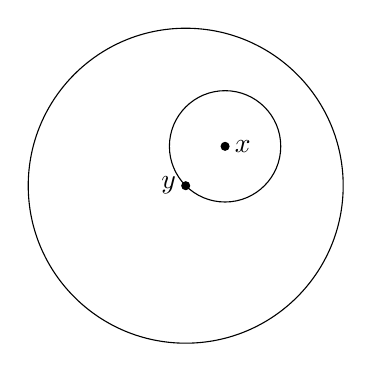
\begin{tikzpicture}
        \filldraw (0.5, 0.5) circle (0.05) node[right] {$x$};
        \draw (0.5, 0.5) circle (0.707);

        \filldraw (0, 0) circle (0.05) node[left] {$y$};
        \draw (0, 0) circle (2);
      \end{tikzpicture}
      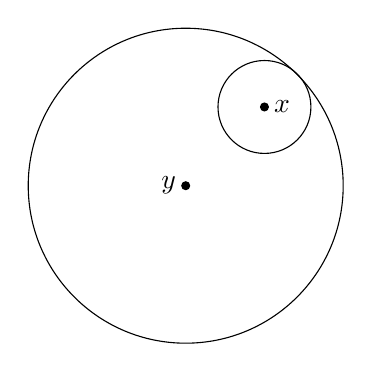
\begin{tikzpicture}
        \filldraw (1, 1) circle (0.05) node[right] {$x$};
        \draw (1, 1) circle (0.59);

        \filldraw (0, 0) circle (0.05) node[left] {$y$};
        \draw (0, 0) circle (2);
      \end{tikzpicture}
    \end{center}
  \end{description}
\end{proof}

\begin{proposition}\label{thm:locally_countable_metric_topology}
  The following is an alternative base for the metric topology\Tinyref{def:metric_topology}:

  \begin{align*}
    \Cal{B}(x) \coloneqq \{ B (x, \tfrac 1 n) \colon n = 1, 2, 3, \ldots \}.
  \end{align*}
\end{proposition}
\begin{proof}
  The proof is the same as in \cref{def:metric_topology}, except for a slight tweak in \ref{thm:topological_local_base_axioms/BP3}, where we define $m$ to be the the smallest positive integer such that
  \begin{align*}
    \tfrac 1 m \leq \min\{ \mu(x, y), r - \mu(x, y) \}.
  \end{align*}

  Note that $m$ exists by \cref{thm:ordinals_are_well_ordered}.

  We then obtain $B(x, \tfrac 1 m) \subseteq B(y, \tfrac 1 n)$.
\end{proof}

\begin{proposition}\label{thm:metric_topology_properties}
  The metric topology $\Cal{T}$ on $X$ induced by $\mu$ has the following properties:
  \begin{defenum}
    \item\label{thm:metric_topology_properties/ball_is_open} For every point $x \in X$ and any radius $r > 0$, the ball $B(x, r)$ is an open set and, hence, a neighborhood of $x$.
    \item\label{thm:metric_topology_properties/first_countable} $\Cal{T}$ is first-countable.
    \item\label{thm:metric_topology_properties/hausdorff} $\Cal{T}$ is Hausdorff.
  \end{defenum}
\end{proposition}
\begin{proof}
  \begin{description}
    \item[\ref{thm:metric_topology_properties/ball_is_open}] Obvious from \cref{def:metric_topology}.

    \item[\ref{thm:metric_topology_properties/first_countable}] Since \cref{thm:locally_countable_metric_topology} involves generating a topology using a neighborhood system of countable local neighborhoods, $\Cal{T}$ is first-countable.

    \item[\ref{thm:metric_topology_properties/hausdorff}] $\Cal{T}$ is Hausdorff by \cref{thm:t2_iff_singleton_limits} since a net.
  \end{description}
\end{proof}

\begin{proposition}\label{thm:metric_convergence_iff_metric_topology_convergence}
  Let $(X, \mu)$ be a metric space and $\Cal{T}$ be the induced metric topology\Tinyref{def:metric_topology}. The convergence\Tinyref{sec:convergence} in $\Cal{T}$ is the completely described by sequences.

  Fix a sequence $\{ x_i \}_{i=1}^\infty$ and consider the sequence as a net\Tinyref{def:topological_net}. Then
  \begin{defenum}
    \item\label{thm:metric_convergence_iff_metric_topology_convergence/cluster_point} $x \in X$ is a cluster point\Tinyref{def:net_cluster_point} of the sequence $\{ x_i \}_{i=1}^\infty$ if and only if for every positive real number $\varepsilon > 0$ and every index $i_0$ there exists an index $i_\varepsilon > i_0$ such that
    \begin{align*}
      \mu(x, x_{i_\varepsilon}) < \varepsilon.
    \end{align*}

    \item\label{thm:metric_convergence_iff_metric_topology_convergence/limit_point} $x \in X$ is a limit point\Tinyref{def:net_limit_point} of the sequence $\{ x_i \}_{i=1}^\infty$ if and only if for every positive real number $\varepsilon > 0$ there exists an index $i_0$ such that
    \begin{align*}
      i \geq i_0 \implies \mu(x, x_i) < \varepsilon.
    \end{align*}

    \item\label{thm:metric_convergence_iff_metric_topology_convergence/closure} Fix a set $A \subseteq X$. A point $x \in X$ belongs to $\Cl{A}$ if and only if there exists a sequence $\{ x_i \}_{i=1}^\infty \subseteq A$ such that $x_i \xrightarrow[i \to \infty]{} x$ (compare with \cref{thm:limit_point_iff_in_closure}).
  \end{defenum}
\end{proposition}
\begin{proof}
  \begin{description}
    \item[\ref{thm:metric_convergence_iff_metric_topology_convergence/cluster_point}] Fix a sequence $x_i \to x$.

    \Implies Fix a radius $\varepsilon > 0$ and an index $i_0$. Note that $B(x, \varepsilon)$ is a neighborhood of $x$ and hence by \cref{def:net_cluster_point} there exists an index $i_\varepsilon \geq i_0$ such that $x_{i_U} \in B(x, \varepsilon)$, which is the same as
    \begin{align*}
      \mu(x, x_{i_U}) < \varepsilon.
    \end{align*}

    \ImpliedBy Fix a neighborhood $U$ of $x$. Since the topology is generated by a local base of balls, then $U$ contains some ball $B(x, r)$. Thus there exists an index $i_0$, such that
    \begin{align*}
      \mu(x, x_{i_r}) < r,
    \end{align*}
    hence
    \begin{align*}
      x_{i_r} \in B(x, r) \subseteq U.
    \end{align*}

    \item[\ref{thm:metric_convergence_iff_metric_topology_convergence/limit_point}] Similar to \ref{thm:metric_convergence_iff_metric_topology_convergence/cluster_point}.

    \item[\ref{thm:metric_convergence_iff_metric_topology_convergence/closure}]
    \Implies Fix a nonempty set $A$ and $x \in \Cl A$. If $x \in A$, then the constant sequence with all members equal to $x$ converges to $A$.

    Assume that $x \not\in A$ and choose any sequence\AOC
    \begin{align*}
      x_i \in B(x, \tfrac 1 i) \setminus \{ x \}, i = 1, 2, \ldots.
    \end{align*}

    Fix $\varepsilon > 0$. By \cref{thm:ordinals_are_well_ordered} there exists a least positive integer $i_0$ such that $\tfrac 1 i_0 < \varepsilon$. It follows that $x_i \to x$ since
    \begin{align*}
      i \geq i_0 \implies \mu(x, x_i) \leq \mu(x, x_{i_0}) \leq \varepsilon.
    \end{align*}

    \ImpliedBy Obvious
  \end{description}
\end{proof}

Let $(X, \rho)$ be a metric space. Let $\B$ be the family of bounded sets in $X$.

Let $(X, \rho)$ be a metric space. Let $\B$ be the family of bounded sets in $X$.

\begin{definition}\label{def:totally_bounded_set}
  The space $A \subseteq X$ is called \uline{totally bounded} if any of the following equivalent conditions hold:

  \begin{defenum}
    \item\label{def:totally_bounded_set/sets} For every $\varepsilon > 0$ there exists a finite cover of $A$ with sets with diameter at most $\varepsilon$.
    \item\label{def:totally_bounded_set/balls} For every $\varepsilon > 0$ there exists a finite cover of $A$ with balls of radius $\varepsilon$.
    \item\label{def:totally_bounded_set/zero_noncompactness/sets} Kuratowski's noncompactness measure (see~\cref{def:noncompactness_measures/sets}) $\alpha(A)$ is zero.
    \item\label{def:totally_bounded_set/zero_noncompactness/balls} The ball noncompactness measure (see~\cref{def:noncompactness_measures/balls}) $\beta(A)$ is zero.
    \item\label{def:totally_bounded_set/fundamental_subsequences} Every sequence in $A$ admits a fundamental subsequence.
  \end{defenum}

  Totally bounded sets are sometimes called \uline{precompact} (see \cref{def:compact_sets}) because of~\cref{thm:metric_sequentially_compact_iff_compact}. This equivalence requires the metric space to be complete, however.
\end{definition}
\begin{proof}
  The equivalences \ref{def:totally_bounded_set/sets} $\iff$ \ref{def:totally_bounded_set/zero_noncompactness/sets} and \ref{def:totally_bounded_set/balls} $\iff$ \ref{def:totally_bounded_set/zero_noncompactness/balls} are straightforward.

  (\ref{def:totally_bounded_set/balls} $\implies$ \ref{def:totally_bounded_set/sets}) Given $\varepsilon > 0$, any cover of $A$ with balls of radius $\frac \varepsilon 2$ is a cover with sets of diameter $\varepsilon$.

  (\ref{def:totally_bounded_set/sets} $\implies$ \ref{def:totally_bounded_set/balls}) Fix $\varepsilon > 0$ and $\mu \in (0, \varepsilon)$ and let $A_1, \ldots, A_n \subseteq \PS X$ be a finite cover of $A$ with sets of diameter at most $\mu$.

  Choose\AOC~a point $x_k$ from every $A_k$, $k = 1, \ldots, n$. We then have that for every $k = 1, \ldots, n$,
  \begin{align*}
    A_k \subseteq \Cl B(x_k, \mu) \subsetneq B(x_k, \varepsilon)
    \\
    \implies A \subseteq \bigcup_{k=1}^n A_k \subseteq \bigcup_{k=1}^n B(x_k, \mu) \subsetneq \bigcup_{k=1}^n B(x_k, \varepsilon),
  \end{align*}
  hence $x_1, \ldots, x_n$ are centers of $\varepsilon$-balls that cover $A$.

  (\ref{def:totally_bounded_set/balls} $\implies$ \ref{def:totally_bounded_set/fundamental_subsequences}) Let $\{ x_n \} \subseteq A$ be any sequence.

  If we assume\LEM\ that $\{ x_n \}$ has no fundamental subsequence, then there exists $\varepsilon_0 > 0$ such that $\rho(x_k, x_m) > \varepsilon_0$ for any $n, m \in \ZPos$.

  Consider a finite cover of $A$ with $\varepsilon_0$-balls. By the pigeonhole principle, at least one of the balls contains more than one element of the sequence, which contradicts the assumption that all elements of the sequence have a distance of at least $\varepsilon_0$.

  Hence an arbitrary sequence in $A$ has a fundamental subsequence.

  (\ref{def:totally_bounded_set/fundamental_subsequences} $\implies$ \ref{def:totally_bounded_set/balls}) Assume\LEM\ that there exists $\varepsilon_0 > 0$, such that $A$ admits no finite cover by $\varepsilon_0$-balls.

  Define $x_1 \in X, x_2 \in X \setminus B(x_1, \varepsilon_0), \ldots$, so that every two elements of the sequence $\{ x_n \}$ have a distance of at least $\varepsilon_0$. But then the sequence is does not admit a fundamental subsequence, which contradicts our assumption.

  This contradiction proves that $A$ admits a finite cover by $\varepsilon$-balls for every $\varepsilon > 0$.
\end{proof}

\begin{corollary}\label{thm:metric_compact_iff_closed_totally_bounded}
  Assume that $X$ is complete. The set $A \subseteq X$ is sequentially compact if and only if it is closed and totally bounded.
\end{corollary}
\begin{proof}
  The property that every sequence has a fundamental subsequence is equivalent to sequential compactness for a closed set in a complete metric space.
\end{proof}

\begin{proposition}\label{thm:closure_of_totally_bounded_is_totally_bounded}
  If a set $A \subseteq X$ is totally bounded, then so is its closure $\Cl A$.
\end{proposition}
\begin{proof}
  Let $\varepsilon > 0$ and $\mu \in (0, \varepsilon)$ and let $x_1, \ldots, x_n \in X$ be the centers of a cover of $A$ with $\mu$-balls.

  If $y$ is a point in $\Cl A \setminus A$, there exists a point $z \in A$ with $\rho(y, z) < \varepsilon - \mu$. Let $x_k \in A$ be one of the centers whose $\mu$-balls contain $z$. We then have that $y \in B(x_k, \varepsilon)$ since
  \begin{align*}
    \rho(x_k, z) \leq \rho(x_k, y) + \rho(y, z) < \mu + \varepsilon - \mu = \varepsilon.
  \end{align*}

  Hence the balls $\Cl B(x_k, \varepsilon)$ cover $\Cl A$, i.e.
  \begin{align*}
    \Cl A \subseteq \bigcup_{k=1}^n B(x_k, \varepsilon).
  \end{align*}
\end{proof}

\begin{lemma}[Lebesgue's covering lemma]\label{thm:lebesgue_covering_lemma}
  Assume that $X$ is complete. Let $A \subseteq X$ be sequentially compact. Given an open cover $\F \subseteq \PS A$, there exists a number $\delta > 0$ such that every $\delta$-ball with a center in $A$ is contained in some set of the cover $\F$.
\end{lemma}
\begin{proof}
  Assume\LEM\ that no such number $\delta > 0$ exists. Then for any natural number $n \in \ZPos$, there exists an element $x_n \in A$ such that the ball $B(x_n, \frac 1 n)$ is not contained in any set of the cover $\F$. Since $A$ is sequentially compact, the sequence $\{ x_n \}_n$ contains a convergent subsequence $\{ x_{n_k} \}_k$.

  Define
  \begin{align*}
    x \coloneqq \lim_{k \to \infty} x_{n_k}.
  \end{align*}

  Let\AOC\ $E$ be a set in $\F$ that contains $x$. Since $E$ is open, there exists some radius $r > 0$ such that $B(x, r) \subseteq E$.

  Choose any $k_0 > \frac 2 r$ such that $\rho(x_{n_{k_0}}, x) < \frac r 2$. By the triangle inequality,
  \begin{align*}
    B \left(x_{n_k}, \frac 1 k \right) \subsetneq B \left(x_k, \frac r 2 \right) \subseteq B(x, r) \subseteq E,
  \end{align*}
  which contradicts the choice of the sequence $\{ x_n \}_n$.

  Hence there exists a $\delta > 0$ such that for every $x \in A$, the ball $B(x, \delta)$ is contained in some element $E$ of the cover $\F$.
\end{proof}

\begin{theorem}\label{thm:metric_compact_iff_sequentially_compact}
  Assume that $X$ is complete. The set $A \subseteq X$ is compact if and only if it is sequentially compact
\end{theorem}
\begin{proof}
  ($\implies$) Let $\F \subseteq \PS X$ be an open cover of $A$.

  By the Lebesgue covering lemma (\cref{thm:lebesgue_covering_lemma}), there exists $\delta > 0$ such that for every $x \in A$, the ball $B(x, \delta)$ is contained in some set of the cover $\F$. Let $x_1, \ldots, x_n$ be a cover of $A$ with $\delta$-balls.

  For each $k = 1, \ldots, n$ we have that the ball $B(x_k, \delta)$ is contained in some set $E_k \in \F$. Hence $E_1, \ldots, E_n$ is a finite subcover of $A$, because
  \begin{align*}
    A \subseteq \bigcup_{k=1}^\infty B(x_k, \delta) \subseteq \bigcup_{k=1}^\infty E_k.
  \end{align*}

  Thus $A$ is compact.

  ($\impliedby$) Let $A$ be compact. Fix $\varepsilon > 0$ and take the cover
  \begin{align*}
    \F \coloneqq \{ B(a, \varepsilon) \colon a \in A \}.
  \end{align*}

  By compactness of $A$, there exists a finite subcover. Thus a finite cover of $A$ with $\varepsilon$-balls exists for every $\varepsilon > 0$. \Cref{def:totally_bounded_set} then implies that total boundedness is equivalent to sequential compactness because $X$ is complete and $A$ is closed.
\end{proof}

\subsection{Noncompactness measures}\label{subsec:noncompactness_measures}

Let \( (X, \mu) \) be a metric space\Tinyref{def:metric_space}. Let \( \Cal{B} \) be the family of bounded sets\Tinyref{def:metric_space/bounded_set} in \( X \).

\begin{definition}\label{def:noncompactness_measures}\cite[definition 7.1]{Deimling1985}
  We define the following functions
  \begin{defenum}
    \DItem{def:noncompactness_measures/sets} The \textbf{Kuratowski measure of noncompactness},
    \begin{align*}
      &\alpha: \Cal{B} \to \BB{R}^{>0} \\
      &\alpha(A) \coloneqq \inf \{d > 0 \colon \exists U_1, \ldots, U_n \subseteq X: \Diam {U_k} < d \land A \subseteq \cup_{k=1}^n U_k \}
    \end{align*}

    \DItem{def:noncompactness_measures/balls} The \textbf{ball measure of noncompactness},
    \begin{align*}
      &\beta: \Cal{B} \to \BB{R}^{>0} \\
      &\beta(A) \coloneqq \inf \{r > 0 \colon \exists x_1, \ldots, x_2 \in X: A \subseteq \cup_{k=1}^n B(x_k, r) \}
    \end{align*}
  \end{defenum}
\end{definition}

\begin{example}\label{ex:noncompactness_measures}\cite[exercise 7.3]{Deimling1985}
  Consider the subsets \( A_2 \subseteq A_3 \subseteq A_1 \subseteq C([0, 1]) \), defined by
  \begin{align*}
    A_1 \coloneqq \left\{
      x \in C([0, 1]) \colon \begin{aligned}
        0 \leq t \leq 1 \implies 0 \leq x(t) \leq 1 \\
        x(0) = 0, x(1) = 1 \\
      \end{aligned}
    \right\}
    \\
    A_2 \coloneqq \left\{
      x \in A_1 \colon \begin{aligned}
        0 \leq t \leq \frac 1 2 \implies 0 \leq x(t) \leq \frac 1 2 \\
        \frac 1 2 \leq t \leq 1 \implies \frac 1 2 \leq x(t) \leq 1
      \end{aligned}
    \right\}
    \\
    A_3 \coloneqq \left\{
      x \in A_1 \colon \begin{aligned}
        0 \leq t \leq \frac 1 2 \implies 0 \leq x(t) \leq \frac 2 3 \\
        \frac 1 2 \leq t \leq 1 \implies \frac 1 3 \leq x(t) \leq 1
      \end{aligned}
    \right\}
  \end{align*}

  Then \( \alpha(A_1) = 1, \alpha(A_2) = \frac 1 2, \alpha(A_3) = \frac 1 3 \) and \( \beta(A_1) = \beta(A_2) = \beta(A_3) = \frac 1 2 \).
\end{example}
\begin{proof}
  Since the distance between any two functions from \( B_1 \) is at most 1, we have that \( \Diam B_1 = 1 \) and \( \alpha(B_1) \leq 1 \).

  Fix \( \varepsilon > 0 \). For any function \( f \in B_1 \), continuity of \( f \) gives us a radius \( \delta_f > 0 \) such that
  \begin{align*}
    x < 2 \delta_f \implies f(x) < \varepsilon.
  \end{align*}

  \begin{figure}[ht]
    \begin{Center}
      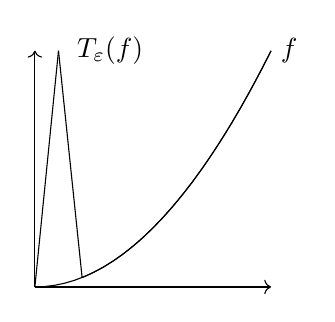
\begin{tikzpicture}[scale=3]
        \draw[->] (0, 0) -- (1, 0);
        \draw[->] (0, 0) -- (0, 1);

        \draw[domain=0:1, variable=\x] plot ({\x}, {\x^2}) node[right] {\( f \)};

        \draw (1/2, 1) node[left] {\( T_\varepsilon(f) \)};
        \draw[domain=0:0.1, variable=\x] plot ({\x}, {10 * \x});
        \draw[domain=0.1:0.2, variable=\x] plot ({\x}, {0.04 + (1 - 0.04) * (2 - 10 * \x)});
        \draw[domain=0.2:1, variable=\x] plot ({\x}, {\x^2});
      \end{tikzpicture}
    \end{Center}
  \end{figure}

  Define
  \begin{align*}
    T_\varepsilon(f)(x) \coloneqq \begin{cases}
      \frac x \delta_f, &0 \leq x < \delta_f \\
      f(\delta_f) + [1 - f(\delta_f)] (2 - \frac x {\delta_f}), &\delta_f \leq x < 2 \delta_f \\
      f(x), &x \geq 2 \delta_f,
    \end{cases}
  \end{align*}
  so that
  \begin{align*}
    \Norm{T_\varepsilon(f) - f}
    \geq
    T_\varepsilon(f) (\delta_f) - f(\delta_f)
    =
    1 - f(\delta_f)
    >
    1 - \varepsilon.
  \end{align*}

  Additionally, because \( \delta_{T_\varepsilon(f)} < \delta_f \), we have that \( f(\delta_{T_\varepsilon(f)}) < \varepsilon \) and
  \begin{align*}
    \Norm{T_\varepsilon(T_\varepsilon(f)) - f}
    \geq
    T_\varepsilon(T_\varepsilon(f)) (\delta_{T_\varepsilon(f)}) - f(\delta_{T_\varepsilon(f)})
    =
    1 - f(\delta_{T_\varepsilon(f)})
    >
    1 - \varepsilon.
  \end{align*}

  Thus, proceeding by induction, we see that for any \( m = 1, 2, \ldots \)
  \begin{align*}
    \Norm{T_\varepsilon^m(f) - f} > 1 - \varepsilon,
  \end{align*}
  where \( T_\varepsilon^m \) denotes repeated application of \( T_\varepsilon \).

  Consider the sequence
  \begin{align*}
    \{ T_\varepsilon^k(f) \}_{k=0}^\infty = \{ f, T_\varepsilon(f), T_\varepsilon(T_\varepsilon(f)), \ldots \}.
  \end{align*}

  We can easily see that the distance between any two elements of the sequence, say \( T_\varepsilon^k(f) \) and \( T_\varepsilon^{k+m}(f) \), is strictly greater that \( 1 - \varepsilon \), i.e.
  \begin{align*}
    \Norm{T_\varepsilon^k(f) - T_\varepsilon^{k+m}(f)}
    =
    \Norm{T_\varepsilon^k(f) - T_\varepsilon^m(T_\varepsilon^k(f))}
    >
    1 - \varepsilon.
  \end{align*}

  Hence \( B_1 \) cannot be covered by a finite \( (1-\varepsilon) \)-net and \( \alpha(B_1) \geq 1 - \varepsilon \). Since \( \varepsilon > 0 \) can be made arbitrarily small, this implies that \( \alpha(B_1) \geq 1 \) and, because we already have the reverse inequality, \( \alpha(B_1) = 1 \).

  In the set \( B_2 \), the maximum distance between two functions is \( \frac 1 2 \), thus \( \Diam(B_2) = \frac 1 2 \) and \( \alpha(B_2) \leq \frac 1 2 \). We can then define an operator similar to \( T_\varepsilon \) that creates \enquote{spikes} of height \( \frac 1 2 \) to prove the reverse inequality, obtaining
  \begin{align*}
    \alpha(B_2) = \frac 1 2.
  \end{align*}

  Finally, the set \( B_3 \) has diameter \( \frac 2 3 \) and hence \( \alpha(B_3) = \frac 2 3 \).

  The ball measure for \( B_1 \) satisfies the inequalities
  \begin{align*}
    \frac 1 2 \leq \beta(B_1) \leq 1.
  \end{align*}

  Additionally, \( B_1 \) is strictly contained in the ball centered in the constant function \( \frac 1 2 \) with radius \( \frac 1 2 \), which implies that \( \beta(B_1) \leq \frac 1 2 \), hence \( \beta(B_1) = \frac 1 2 \).

  For \( B_2 \) we have
  \begin{align*}
    \frac 1 4 \leq \beta(B_2) \leq \frac 1 2.
  \end{align*}

  Assume\LEM that for some \( \varepsilon > 0 \) the set \( B_2 \) can be covered by a finite set of balls with centers \( \{ f_1, \ldots, f_n \} \subsetneq C([0, 1]) \) and radius \( \frac 1 2 - \varepsilon \).

  Because of continuity, we can find a radius \( \delta > 0 \) such that for all \( f_k, k = 1, \ldots, n \) we have
  \begin{align*}
    x \in \left[\tfrac {1 - \delta} 2, \tfrac {1 + \delta} 2 \right] \implies \Abs{f_k(x) - f_k(\tfrac 1 2)} < \varepsilon.
  \end{align*}

  Consider the function
  \begin{align*}
    g(x) \coloneqq \begin{cases}
      0, &0 \leq x < \frac {1 - \delta} 2, \\
      \frac{2x + \delta - 1} {2\delta}, &\frac {1 - \delta} 2 \leq x \leq \frac {1 + \delta} 2, \\
      1, &\frac {1 + \delta} 2 < x \leq 1.
    \end{cases}
  \end{align*}

  \begin{figure}[ht]
    \begin{Center}
      \begin{tikzpicture}[scale=5]
        \draw[->] (0, 0) -- (1, 0);
        \draw[->] (0, 0) -- (0, 1);
        \draw[domain=0:4/10, thick, variable=\x] plot ({\x}, {0});
        \draw[domain=4/10:6/10, thick, variable=\x] plot ({\x}, {5 * \x - 2}) node[left] {\( g \)};
        \draw[domain=6/10:1, thick, variable=\x] plot ({\x}, {1});

        \draw[densely dotted] (0, 6/10) node[left] {\( f_k(\frac 1 2) - \varepsilon \)} -- (1, 6/10);
        \draw[densely dotted] (0, 8/10) node[left] {\( f_k(\frac 1 2) + \varepsilon \)} -- (1, 8/10);

        \draw[densely dotted] (4/10, 0) -- (4/10, 1);
        \draw (3/10, -1/10) node {\( \frac {1 - \delta} 2 \)};
        \draw[densely dotted] (1/2, 0) -- (1/2, 1);
        \draw (1/2, -1/10) node {\( \frac 1 2 \)};
        \draw[densely dotted] (6/10, 0) -- (6/10, 1);
        \draw (7/10, -1/10) node {\( \frac {1 + \delta} 2 \)};

        \draw[domain=-1/10:1, dash dot, variable=\x] plot ({\x}, {2/10 + 1 / (1 + e^(5/3*(1-2*\x)))}) node[right] {\( f_k \)};
      \end{tikzpicture}
    \end{Center}
  \end{figure}

  If \( f_k(\tfrac 1 2) \geq \frac 1 2 \), then \( f_k(\tfrac {1 - \delta} 2) > \tfrac 1 2 - \varepsilon \) and
  \begin{align*}
    \Norm{f_k - g} \geq f_k(\tfrac {1 - \delta} 2) - g(\tfrac {1 - \delta} 2) = f_k(\tfrac {1 - \delta} 2) > \tfrac 1 2 - \varepsilon.
  \end{align*}

  Analogously, if \( f_k(\tfrac 1 2) < \frac 1 2 \), then \( f_k(\tfrac {1 + \delta} 2) < \tfrac 1 2 + \varepsilon \) and
  \begin{align*}
    \Norm{g - f_k} \geq g(\tfrac {1 + \delta} 2) - f_k(\tfrac {1 + \delta} 2) = 1 - f_k(\tfrac {1 + \delta} 2) > \tfrac 1 2 - \varepsilon.
  \end{align*}

  Thus, for every \( k = 1, \ldots, n \) we have
  \begin{align*}
    \Norm{g - f_k} > \frac 1 2 - \varepsilon,
  \end{align*}
  i.e. \( g \) in not contained in a ball of radius \( \frac 1 2 - \varepsilon \) around any of the centers \( f_1, \ldots, f_n \).

  Hence \( \beta(B_2) \geq \frac 1 2 \), which implies \( \beta(B_2) = \frac 1 2 \). Because of the inclusion \( B_2 \subsetneq B_3 \subsetneq B_1 \), we have
  \begin{align*}
    \frac 1 2 = \beta(B_2) \leq \beta(B_3) \leq \beta(B_1) = \frac 1 2,
  \end{align*}
  hence \( \beta(B_3) = \frac 1 2 \).
\end{proof}

\begin{theorem}\label{thm:noncompact_kuratowski_lemma}[Kuratowski lemma]\cite[exercise 7.4]{Deimling1985}
  Let \( X \) be a Banach space and \( \{ A_n \}_n \) be a decreasing sequence of nonempty closed subsets such that \( \alpha(A_n) \to 0 \). Then \( A \coloneqq \bigcap_n A_n \) is nonempty and compact.
\end{theorem}
\begin{proof}
  The set \( A \) is compact because it is closed as the intersection of closed sets and \( \alpha(A) \leq \alpha(A_n) \to 0 \), hence \( \alpha(A) = 0 \).

  It remains to show that \( A \) is nonempty.
  Choose\AOC any sequence \( \{ x_n \}_n \) where \( x_n \in A_n \). Since any finite set is compact, we have that for any \( k \geq 1 \)
  \begin{align*}
    \alpha(\{ x_n \}_{n \geq 1})
    =
    \max\{ \alpha(\{ x_n \}_{n < k}), \alpha(\{ x_n \}_{n \geq k}) \}
    =
    \alpha(\{ x_n \}_{n \geq k})
    \leq
    \alpha(A_k) \to 0,
  \end{align*}
  hence the set \( \{ x_n \colon n \geq 1 \} \) is compact and thus sequentially compact. We can choose a convergent subsequence \( \{ x_{n_k} \}_k \) of \( \{ x_n \}_n \) whose limit lies in every \( A_n \) (since they are closed) and, consequently, in their intersection \( A \). So \( A \) is nonempty.
\end{proof}


\section{Logic}\label{sec:logic}
\subsection{Languages}\label{subsec:languages}

Languages are used to define formulas for expressing the axioms of set theory\Tinyref{def:set_zfc}. Here, sets are used to formally define languages. This vicious cycle is left to logicians.

\begin{definition}\label{def:language}
  Given a set \( \Cal{A} \), called an \textbf{alphabet}, whose elements are called \textbf{symbols}, we define a \textbf{word} or \textbf{string} over \( \Cal{A} \) to be any tuple\Tinyref{def:cartesian_product} of symbols. Words are written simply as strings of symbols, that is, \( abc \) instead of \( (a, b, c) \). The empty word with no symbols is usually denoted by \( \varepsilon \).

  The set of all (finite) words over \( \Cal{A} \) is denoted by \( \Cal{A}^{*} \). The operation \( * \) is called the \textbf{Kleene star}. A \textbf{language} \( \Cal{L} \) is any subset of \( \Cal{A}^{*} \).

  We define two functions:
  \begin{align*}
    &\Len: \Cal{A}^{*} \to \BB{Z}^{\geq 0}
    &&\cdot: \Cal{A}^{*} \to \BB{Z}^{\geq 0}
    \\
    &\Len(w) \coloneqq \text{length of the tuple } w
    &&v \cdot w \coloneqq (v_1, \ldots, v_{\Len(v)}, w_1, \ldots, w_{\Len(w)}).
  \end{align*}

  The function \( v \cdot w \) is called \textbf{concatenation} and is usually denoted by juxtaposition. It is obviously associative.

  We say that \( p \) is a \textbf{prefix} of \( w \) if the first \( \Len(p) \) symbols of \( w \) are identical to those of \( p \), that is,
  \begin{align*}
    w = (p_1, \ldots, p_{\Len(p)}, w_{\Len(p) + 1}, \ldots, w_{\Len(w)}).
  \end{align*}

  \textbf{Suffixes} are defined analogously. We say that \( v \) is a \textbf{subword} of \( w \) if there exists a prefix \( p \) and a suffix \( s \) such that \( w = pvs \). We define the partial order\Tinyref{def:order/partial} \( v \leq w \iff v \) is a subword of \( w \).

  Evidently both prefixes and suffixes are subwords and \( v \leq w \iff \Len(v) \leq \Len(w) \).

  For convenience, we denote \textbf{runs of length \( n \)} of some letter \( a \) as \( a^n \), that is,
  \begin{align*}
    a^n \coloneqq \begin{cases}
      \varepsilon, &n = 0, \\
      a a^{n-1}, &n > 1.
    \end{cases}
  \end{align*}

  Thus we do not distinguish between the words \( aaabbaa \) and \( a^3 b^2 a^2 \).
\end{definition}

\begin{proposition}\label{thm:set_of_all_words_is_monoid}
  For any alphabet \( \Cal{A} \), the language \( (\Cal{A}^{*}, \cdot) \) is a monoid.
\end{proposition}

\subsection{Grammars}\label{subsec:grammars}

\begin{definition}\label{def:grammar}\MarginCite[def. 2.2]{Sipser2013}
  Let \( \Cal{A} \) be some \hyperref[def:language/alphabet]{alphabet} and \( V, \Sigma \subseteq \Cal{A} \) be nonempty disjoint subsets of \( \Cal{A} \).

  \begin{DefEnum}
    \ILabel{def:grammar/variables} We call elements of \( V \) \Def{variables} or \Def{non-terminals}.

    \ILabel{def:grammar/terminals} We call elements of elements of \( \Sigma \) \Def{terminals}.

    \ILabel{def:grammar/start} We assume that a special \Def{start symbol} \( S \in V \) is fixed.

    \ILabel{def:grammar/production_rules} We define a binary \hyperref[def:relation]{relation} \( \to \) of \Def{production rules} over \( (V \cup \Sigma)^* \), that is, rules are \enquote{transformations} that define how a language is \enquote{generated} starting from \( S \in V \) (see \fullref{def:grammar_derivation} and \fullref{ex:def:grammar/arithmetic}). By convention, we treat uppercase symbols as variables and lowercase symbols as terminals. See, for example, \fullref{remark:backus_naur_form}. When speaking about general grammars, however, we usually use the letters \( u \), \( v \) and \( w \) to denote words (that may contain variables) rather than terminals.

    \ILabel{def:grammar/terminal_rules} Rules of the form \( u \to \sigma \), where \( \sigma \in \Sigma \), are called \Def{terminal rules}. Note that \( u \) here is a word and not a terminal.

    \ILabel{def:grammar/grammar} The tuple \( G \coloneqq (V, \Sigma, \to, S) \) is called a \Def{formal grammar}.

    \ILabel{def:grammar/context_free} If every production rule has only a single variable for a source, i.e. if for every rule \( u \to v \) we have \( u = A \) for some \( A \in V \), we say that the grammar is \Def{context-free}.
  \end{DefEnum}
\end{definition}

\begin{remark}\label{remark:backus_naur_form}
  In practice, specifying a \hyperref[def:grammar/context_free]{context-free grammar} as
  \begin{AlignedEquation}\label{eq:remark:backus_naur_form/long_rule_list}
    &A \to a, \\
    &A \to b, \\
    &A \to AC, \\
    &C \to c,
  \end{AlignedEquation}
  or even via the shorthand notation
  \begin{AlignedEquation}\label{eq:remark:backus_naur_form/short_rule_list}
    &A \to a \mid b \mid AC, \\
    &C \to c, \\
  \end{AlignedEquation}
  quickly becomes cumbersome.

  When dealing with more complicated languages like \hyperref[def:first_order_language/grammar]{first-order formulas}, and especially when dealing with programming languages (e.g. the Python grammar that can be found in \cite{Python:39_grammar}), it is more convenient to use alternative notation like the \Def{Backus-Naur form (BNF)}. It is a metasyntax, i.e. a syntax for describing language syntax.

  Compared to \eqref{eq:remark:backus_naur_form/long_rule_list}, the main differences are:
  \begin{enumerate}
    \item Variables are denoted by \( \langle \) words enclosed in angle brackets \( \rangle \) so that we can name variables using more than one symbol.
    \item Terminals are denoted using \enquote{quotes}. In human-readable rich text documents like this one, it is sometimes possible to use different fonts and so instead of \enquote{quotes} we specify terminals using an \texttt{upright monospaced font}.
    \item Free-text rules can be specified using a normal font. This is also only used in human-readable rich text documents, however this usage is justified because such rules are only beneficial for human understanding and not for machine parsing.
    \item The symbol \( :\coloneqq \) is used instead of \( \to \) for specifying transition rules.
    \item Different rules with the same source are concatenated as in \eqref{eq:remark:backus_naur_form/short_rule_list}.
  \end{enumerate}

  For example, \eqref{eq:remark:backus_naur_form/long_rule_list} becomes
  \begin{bnf*}
    \bnfprod{A} {\bnfts{a} \bnfor \bnfts{b} \bnfor \bnfpn{A} \bnfpn{C}} \\
    \bnfprod{C} {\bnfts{c}}
  \end{bnf*}
\end{remark}

\begin{definition}\label{def:grammar_derivation}\MarginCite[page 104 \\ page 108]{Sipser2013}
  Fix a \hyperref[def:grammar]{formal grammar} \( G = (V, \Sigma, \to, S) \). Note that all lowercase symbols in this definitions are words rather than terminals.

  \begin{DefEnum}
    \ILabel{def:grammar_derivation/yields} Fix a \hyperref[def:language/word]{word} \( pvs \). If \( u \to v \) is a production rule, we say that \( pvs \) \Def{yields} the word \( pws \) and write
    \begin{equation*}
      pvs \Rightarrow pws.
    \end{equation*}

    \ILabel{def:grammar_derivation/derivation} We say that \( u \) \Def{derives} \( v \) and write \( u \Rightarrow v \) if there exists a finite sequence of words \( u_1, \ldots, u_n \) such that
    \begin{equation*}
      u \Rightarrow u_1 \Rightarrow \ldots \Rightarrow u_n \Rightarrow v.
    \end{equation*}

    The sequence \( u, u_1, \ldots, u_n, v \) is called a \Def{derivation} of \( v \) from \( u \).

    \ILabel{def:grammar_derivation/leftmost_rightmost_derivation} If on every step of the derivation the leftmost (resp. rightmost) variable is replaced, we say that it is a \Def{leftmost} (resp. \Def{rightmost}) derivation.

    \ILabel{def:grammar_derivation/grammar_language} Define the \Def{language} of the grammar to be
    \begin{equation*}
      \Cal{L}(G) \coloneqq \{ w \in \Sigma^* \colon S \Rightarrow w \},
    \end{equation*}
    that is, all words that can be derived from \( S \) and contains only terminals.

    We also say that strings in \( \Cal{L}(G) \) are \Def{generated} by the grammar \( G \).

    \ILabel{def:grammar_derivation/ambiguity}\MarginCite[def. 2.7]{Sipser2013}We say that the word \( w \) can be derived \Def{unambiguously} if there exists a unique leftmost derivation from \( S \). Otherwise we say that \( w \) is generated \Def{ambiguously} and that the grammar itself is \Def{ambiguous}.
  \end{DefEnum}
\end{definition}

\begin{example}\label{ex:def:grammar/arithmetic}
  We will define a grammar for addition on \hyperref[def:natural_numbers]{natural numbers}. Note that we only consider the number in \( \BN \) only as symbols, not as the numbers themselves.

  Let \( V \coloneqq \{ A \} \) and \( \Sigma \coloneqq \BN \cup \{ +, (, ) \} \). Define the grammar
  \begin{AlignedEquation}\label{eq:ex:context_free_grammar/real_arithmetic/grammar}
    &A \to n,                 && n \in \BN \\
    &A \to (A + A)            &&
  \end{AlignedEquation}

  Choose the starting symbol to be the only symbol \( A \) in \( V \). Then the grammar can produce the arithmetic expression \( ((1 + 2) + 3) \) by applying the rules
  \begin{equation*}
    \begin{mplibcode}
      u := 2cm;

      beginfig(1);
      input metapost/graphs;

      v1 := thelabel("$A$", origin);
      v2 := thelabel("$(A + A)$", (0, -1) scaled u);
      v3 := thelabel("$3$", (1, -2) scaled u);
      v4 := thelabel("$(A + A)$", (-1, -2) scaled u);
      v5 := thelabel("$1$", (-2, -3) scaled u);
      v6 := thelabel("$2$", (0, -3) scaled u);

      a1 := straight_arc(v1, v2);
      a2 := straight_arc(v2, v3);
      a3 := straight_arc(v2, v4);
      a4 := straight_arc(v4, v5);
      a5 := straight_arc(v4, v6);

      draw_vertices(v);
      draw_arcs(a);

      label.lft("$A \to (A + A$)", straight_arc_midpoint of a1);
      label.urt("$A \to 3$", straight_arc_midpoint of a2);
      label.ulft("$A \to (A + A)$", straight_arc_midpoint of a3);
      label.ulft("$A \to 1$", straight_arc_midpoint of a4);
      label.urt("$A \to 2$", straight_arc_midpoint of a5);
      endfig;
    \end{mplibcode}
  \end{equation*}

  Note that the grammar is unambiguous because of the parentheses. If we omit the parentheses, it will no longer be unambiguous since \( 1 + 2 + 3 \) can be derived by both
  \begin{equation*}
    \begin{mplibcode}
      u := 2cm;

      beginfig(1);
      input metapost/graphs;

      v1 := thelabel("$A$", origin);
      v2 := thelabel("$A + A$", (0, -1) scaled u);
      v3 := thelabel("$1$", (-1, -2) scaled u);
      v4 := thelabel("$A + A$", (1, -2) scaled u);
      v5 := thelabel("$2$", (0, -3) scaled u);
      v6 := thelabel("$3$", (2, -3) scaled u);

      a1 := straight_arc(v1, v2);
      a2 := straight_arc(v2, v3);
      a3 := straight_arc(v2, v4);
      a4 := straight_arc(v4, v5);
      a5 := straight_arc(v4, v6);

      draw_vertices(v);
      draw_arcs(a);

      label.lft("$A \to A + A$", straight_arc_midpoint of a1);
      label.ulft("$A \to 1$", straight_arc_midpoint of a2);
      label.urt("$A \to A + A$", straight_arc_midpoint of a3);
      label.ulft("$A \to 2$", straight_arc_midpoint of a4);
      label.urt("$A \to 3$", straight_arc_midpoint of a5);
      endfig;
    \end{mplibcode}
    \hspace{1cm}
    \begin{mplibcode}
      u := 2cm;

      beginfig(1);
      input metapost/graphs;

      v1 := thelabel("$A$", origin);
      v2 := thelabel("$A + A$", (0, -1) scaled u);
      v3 := thelabel("$3$", (1, -2) scaled u);
      v4 := thelabel("$A + A$", (-1, -2) scaled u);
      v5 := thelabel("$1$", (-2, -3) scaled u);
      v6 := thelabel("$2$", (0, -3) scaled u);

      a1 := straight_arc(v1, v2);
      a2 := straight_arc(v2, v3);
      a3 := straight_arc(v2, v4);
      a4 := straight_arc(v4, v5);
      a5 := straight_arc(v4, v6);

      draw_vertices(v);
      draw_arcs(a);

      label.lft("$A \to A + A$", straight_arc_midpoint of a1);
      label.urt("$A \to 3$", straight_arc_midpoint of a2);
      label.ulft("$A \to A + A$", straight_arc_midpoint of a3);
      label.ulft("$A \to 1$", straight_arc_midpoint of a4);
      label.urt("$A \to 2$", straight_arc_midpoint of a5);
      endfig;
    \end{mplibcode}
  \end{equation*}
\end{example}
\begin{proof}
  We will show that \( G \) is unambiguous. Let \( w \) be a word in \( \Cal{L}(G) \). We explicitly build the derivation of \( w \) by induction\IND on \( \Len(w) \):
  \begin{itemize}
    \item If \( \Len(w) = 1 \), then \( w = n \in \BN \) and the word has been generated by the single rule \( A \to n \).

    \item Assume that \( w \) is unambiguously derived for \( \Len(w) < m + 2 \) and let \( \Len(w) = m + 2 \), then \( w \) is necessarily enclosed in parentheses. Let \( w = ( \sigma_0 \ldots \sigma_m ) \) be the symbols of \( w \). Because of the parentheses, the only possibility for \( \sigma_0 \ldots \sigma_m \) is that it consists of two words in \( \Cal{L}(G) \) with an addition symbol \( + \) between them. Let \( k \) be the index of the operator, that is, the index such that \( \sigma_1 \ldots \sigma_{k-1} \) and \( \sigma_{k+1} \ldots \sigma_m \) both belong to \( \Cal{L}(G) \). Furthermore, by inductive hypothesis, both \( \sigma_1 \ldots \sigma_{k-1} \) and \( \sigma_{k+1} \ldots \sigma_m \) are unambiguously derived. Therefore \( w \) is also unambiguously derived.
  \end{itemize}
\end{proof}

\subsection{Propositional logic}\label{subsec:propositional_logic}

\begin{remark}\label{remark:metalanguage}
  Mathematical logic uses mathematics to study languages that themselves describe mathematics. Thus a distinction should be made between \Def{the language} under study, and \Def{the metalanguage} which we use to write statements relating to the language under study. This distinction is often emphasized by using different logical symbols in the two languages. We do not force such a distinction since it is often clear from the context which language the symbol belongs to.

  Outside of logic, \fullref{def:propositional_logic_language/connectives} are frequently used, however the use of connectives in statements in the metalanguage within logic can be reduced to a minimum and not cause any confusion. At the same time, \fullref{def:propositional_logic_language/constants} are used both in the language and in the metalanguage, so we use the following convention:
  \begin{itemize}
    \item the \( \top \) and \( \bot \) symbols represent truth and false values in the language.
    \item the \( T \) and \( F \) symbols represent truth and false values in the metalanguage.
  \end{itemize}

  We denote equality in the language by \( \doteq \).
\end{remark}

\begin{definition}\label{def:propositional_logic_language}\cite[102]{OpenLogic20201202}
  Propositional logic is a simple framework for describing relationships between statements. It is sometimes called boolean logic because of \fullref{thm:propositional_logic_boolean_algebra}.

  The language\Tinyref{def:language} of propositional logic consists of \Def{propositional formulas}, which are certain well-formed words over the alphabet consisting of
  \begin{description}
    \DItem{def:propositional_logic_language/prop}(propositional variables) A nonempty set \( \Cat{Prop} \) of \Def{propositional variables}.

    \DItem{def:propositional_logic_language/constants}(propositional constants)\mbox{}
    \begin{description}
      \DItem{def:propositional_logic_language/top}(top) \( \top \)
      \DItem{def:propositional_logic_language/bottom}(bottom) \( \bot \)
    \end{description}

    \DItem{def:propositional_logic_language/negation}(negation) \( \neg \)
    \DItem{def:propositional_logic_language/connectives}(propositional connectives) The set \( \Sigma \) of \Def{propositional connectives}, namely
    \begin{description}
      \DItem{def:propositional_logic_language/conjunction}(conjunction (and)) \( \land \)
      \DItem{def:propositional_logic_language/disjunction}(disjunction (or)) \( \lor \)
      \DItem{def:propositional_logic_language/implication}(implication) \( \implies \)
      \DItem{def:propositional_logic_language/equivalence}(equivalence) \( \iff \)
      \DItem{def:propositional_logic_language/pierce_arrow}(Pierce's arrow (nor)) \( \downarrow \)
      \DItem{def:propositional_logic_language/sheffer_stroke}(Sheffer stroke (nand)) \( \uparrow \)
    \end{description}

    \DItem{def:propositional_logic_language/parentheses}(parentheses) Parentheses \( ( \) and \( ) \) for defining the order of operations unambiguously (see \fullref{remark:propositional_formula_parentheses}).
  \end{description}

  The propositional formulas \( \Cal{F}_B \) are defined inductively as
  \begin{itemize}
    \item the variables in \( \Cat{Prop} \) are formulas.
    \item the constants \( \top \) and \( \bot \) are formulas.
    \item if \( \varphi \) is a formula, then \( \neg \varphi \) is a formula.
    \item if \( \varphi \) and \( \psi \) are formulas, so are \( (\varphi \circ \psi) \), where \( \circ \in \Sigma \).
  \end{itemize}

  Furthermore, the grammar of propositional formulas is unambiguous (see \fullref{thm:propositional_formulas_are_unambiguous}).

  If \( \varphi \) and \( \psi \) are formulas and \( \psi \) is a subword of \( \varphi \), we say that \( \psi \) is a \Def{subformula} of \( \varphi \).

  For each formula \( \varphi \), we define the set of its variables as
  \begin{align*}
    \Cat{Var}(\varphi) \coloneqq \begin{cases}
      \varnothing,                              &\varphi \in \{ \top, \bot \} \\
      \{ P \},                                  &\varphi = P \in \Cat{Prop} \\
      \Cat{Var}(\psi),                         &\varphi = \neg \psi \\
      \Cat{Var}(\psi) \cup \Bold{Var}(\theta), &\varphi = (\psi \circ \theta), \circ \in \Sigma.
    \end{cases}
  \end{align*}
\end{definition}

\begin{definition}\label{def:truth_functions}
  We define the following truth functions
  \begin{equation*}
    \begin{tabular}{c | c || c c | c c c c c c}
      \( x \)    & \( H_\neg \) & \( x \)    & \( y \)    & \( H_\lor \) & \( H_\land \) & \( H_\Rightarrow \) & \( H_{\iff} \) & \( H_\downarrow \) & \( H_\uparrow \) \\
      \hline
      \( T \)    & \( F \)      & \( T \)    & \( T \)    & \( T \)      & \( T \)       & \( T \)          & \( T \)      & \( F \)            & \( F \)    \\
      \( F \)    & \( T \)      & \( T \)    & \( F \)    & \( T \)      & \( F \)       & \( F \)          & \( F \)      & \( F \)            & \( T \)    \\
             &          & \( F \)    & \( T \)    & \( T \)      & \( F \)       & \( T \)          & \( T \)      & \( F \)            & \( T \)    \\
             &          & \( F \)    & \( F \)    & \( F \)      & \( F \)       & \( T \)          & \( F \)      & \( T \)            & \( T \)
    \end{tabular}
  \end{equation*}
\end{definition}

\begin{definition}\label{def:propositional_substition}
  If \( \varphi \) and \( \rho \) are formulas and \( \psi \) is a subformula of \( \varphi \), we define the \Def{substition} of \( \psi \) with \( \rho \) in \( \varphi \) as
  \begin{align*}
    \varphi[\psi \to \rho] &\coloneqq \begin{cases}
      \rho,                                                    &\varphi = \psi \\
      \varphi,                                                 &\varphi \neq \psi \text{ and } \varphi \in \{ \top, \bot \} \cup \Cat{Prop} \\
      \neg \theta[\psi \to \rho],                              &\varphi \neq \psi \text{ and } \varphi = \neg \theta \\
      (\theta_1[\psi \to \rho] \circ \theta_2[\psi \to \rho]), &\varphi \neq \psi \text{ and } \varphi = (\theta_1 \circ \theta_2), \circ \in \Sigma.
    \end{cases}
  \end{align*}

  We will now define \Def{simultaneous substition} of \( \psi_1, \ldots, \psi_n \) with \( \rho_1, \ldots, \rho_n \). The problem with iterated substition that we wish to avoid is if \( \psi_i \) is a subformula of \( \rho_{i-1} \) and accidentally gets replaced during \( \varphi[\psi_{i-1} \to \rho_{i-1}][\psi_i \to \rho_i] \).

  Define
  \begin{equation*}
    \Cat{Bound} \coloneqq \Bold{Var}(\rho_1) \cup \ldots \cup \Bold{Var}(\rho_n).
  \end{equation*}
  and, for each variable \( P_i \) in \( \Cat{Bound} \), choose\AOC a variable \( Q_i \) from \( \Bold{Prop} \setminus \Bold{Bound} \). Let \( m \) be the cardinality of \( \Bold{Bound} \). The simultaneous substitution can then be defined as
  \begin{align*}
    \varphi[\psi_1 \to \rho_1, \ldots, \psi_n \to \rho_n] \coloneqq \varphi
    [\psi_1 \to \rho_1[P_1 \to Q_1, \ldots, P_m \to Q_m]] \\
    \ldots \\
    [\psi_n \to \rho_n[P_1 \to Q_1, \ldots, P_m \to Q_m]] \\
    [Q_1 \to P_1, \ldots, Q_m \to P_m].
  \end{align*}
\end{definition}

\begin{remark}\label{remark:propositional_formula_parentheses}
  We often omit parentheses from propositional formulas when no conceptual ambiguity is possible, for example we often write \( \varphi \land \psi \land \theta \) instead of \( ((\varphi \land \psi) \land \theta) \). These are only notations shortcuts in the metalanguage\Tinyref{remark:metalanguage} and the formulas themselves (as abstract mathematical objects) are still assumed to contain parentheses to avoid syntactic ambiguity (see \fullref{thm:propositional_formulas_are_unambiguous}).
\end{remark}

\begin{proposition}\label{thm:propositional_formulas_are_unambiguous}
  The grammar\Tinyref{def:grammar} of propositional logic formulas\Tinyref{def:propositional_logic_language}
  \begin{displaymath}
    \begin{aligned}
      &\Phi \to p,                 &&p \in \Cat{Prop} \\
      &\Phi \to \top \;|\; \bot    && \\
      &\Phi \to \neg \Phi          && \\
      &\Phi \to (\Phi \circ \Phi), &&\circ \in \Sigma.
    \end{aligned}
  \end{displaymath}
  is unambiguous\Tinyref{def:ambiguous_grammar}.
\end{proposition}
\begin{proof}
  The proof is analogous to \fullref{ex:context_free_grammar/real_arithmetic}.
\end{proof}

\begin{remark}\label{remark:minimal_propositional_language}
  By \fullref{ex:posts_completeness_theorem/nand}, it is actually sufficient for propositional logic to only have
  \begin{itemize}
    \item \fullref{def:propositional_logic_language/prop}.
    \item \fullref{def:propositional_logic_language/pierce_arrow} \( \downarrow \) or the \fullref{def:propositional_logic_language/sheffer_stroke} \( \uparrow \) (we will use the arrow \( \downarrow \)).
    \item \fullref{def:propositional_logic_language/parentheses}.
  \end{itemize}

  We are able to expand the language and define the constants, negation and all other connectives so that the truth functions in \fullref{def:truth_functions} are satisfied. This can simplify the study of propositional logic itself.

  Equivalence is a bit tricky to define since we use it to define the other logical operations. We choose\AOC two variables \( P \) and \( Q \) and define an auxiliary formula that expresses the equivalence \( P \iff Q \) through Pierce's arrow:
  \begin{equation*}
    \lambda \coloneqq (P \downarrow (Q \downarrow Q)) \downarrow (Q \downarrow (P \downarrow P)).
  \end{equation*}
 or \fullref{def:algebraic_theory}
  In order to simplify our discussion, we can assume that the following axioms always hold (see \fullref{def:propositional_theory}) for all formulas \( \varphi \) and \( \psi \):
  \begin{description}
    \RItem{def:propositional_logic_language/equivalence} \( \lambda[P \to (\varphi \iff \psi), Q \to \lambda[P \to \varphi, Q \to \psi]] \)
    \RItem{def:propositional_logic_language/negation} \( \neg \varphi \iff (\varphi \downarrow \varphi) \)
    \RItem{def:propositional_logic_language/conjunction} \( (\varphi \land \psi) \iff ((\varphi \downarrow \varphi) \downarrow (\psi \downarrow \psi)) \)
    \RItem{def:propositional_logic_language/disjunction} \( (\varphi \lor \psi) \iff \neg (\varphi \downarrow \psi) \)
    \RItem{def:propositional_logic_language/top} \( \top \iff (\varphi \land \varphi) \)
    \RItem{def:propositional_logic_language/bottom} \( \bot \iff \neg \top \)
    \RItem{def:propositional_logic_language/implication} \( (\varphi \implies \psi) \iff (\neg \varphi \lor \psi) \)
    \RItem{def:propositional_logic_language/sheffer_stroke} \( (\varphi \uparrow \psi) \iff \neg (\varphi \land \psi) \)
  \end{description}

  The proofs of these equivalences can be easily verified using the truth tables in \fullref{def:truth_functions}.
\end{remark}

\begin{definition}\label{def:conjunctive_normal_form}
  We define \Def{literals} to either be propositional variables \( L = P \) or negations \( L = \neg P \) of propositional variables.

  We define \Def{disjuncts} (resp. \Def{conjuncts}) to be finite disjunctions (resp. conjunctions) of literals, i.e.
  \begin{equation*}
    L_1 \lor L_2 \lor \ldots \lor L_n.
  \end{equation*}

  We say that a propositional formula \( \varphi \) is in \Def{conjunctive normal form} (resp. \Def{disjunctive normal form}) if \( \varphi \) is a finite conjunction of disjunctions (resp. finite disjunction of conjunctions).
\end{definition}

\begin{proposition}\label{thm:conjunctive_normal_form_reduction}
  Every propositional formula \( \varphi \) is Boolean equivalent\Tinyref{def:propositional_interpretation} to a formula in conjunctive normal form\Tinyref{def:conjunctive_normal_form}.
\end{proposition}

\begin{definition}\label{def:propositional_interpretation}
  A \Def{propositional interpretation} is a function \( I: \Cat{Prop} \to \{ T, F \} \).

  We define interpretation for formulas inductively as
  \begin{align*}
    \varphi[I] \coloneqq \begin{cases}
      T,                           &\varphi = \top \\
      F,                           &\varphi = \bot \\
      I(P),                        &\varphi = P \in \Cat{Prop} \\
      H_\neg(\psi[I]),             &\varphi = \neg \psi         \\
      H_\circ(\psi[I], \theta[I]), &\varphi = \psi \circ \theta, \circ \in \Sigma.
    \end{cases}
  \end{align*}

  We say that
  \begin{defenum}
    \DItem{def:propositional_interpretation/model} \( I \) is a \Def{Boolean model} of \( \varphi \) and write \( I \models_B \varphi \) if \( \varphi[I] = T \).
    \DItem{def:propositional_interpretation/entailment} the set \( \Gamma \) of formulas \Def{entail} the formula \( \varphi \) (denoted as \( \Gamma \models_B \varphi \)) if every model for \( \Gamma \) is a model for \( \varphi \).
    \DItem{def:propositional_interpretation/tautology} \( \varphi \) is a \Def{tautology} if all interpretations are models for \( \varphi \).
    \DItem{def:propositional_interpretation/contradiction} \( \varphi \) is a \Def{contradiction} if no interpretation is a model for \( \varphi \).
    \DItem{def:propositional_interpretation/equivalence} \( \varphi \) and \( \psi \) are \Def{Boolean equivalent} and write \( \varphi \equiv_B \psi \) if \( \varphi[I] = \psi[I] \) for any interpretation \( I \).
  \end{defenum}
\end{definition}

\begin{definition}\label{def:propositional_theory}\cite[definition 15.1]{OpenLogic20201202}
  The \Def{closure} of a set of formulas \( \Gamma \) is defined as
  \begin{equation*}
    \Cl(\Gamma) \coloneqq \{ \varphi(x) \colon \Gamma \models_B \varphi \}.
  \end{equation*}

  A set of formulas is said to be \Def{closed} if it coincides with its closure.

  If \( \Delta \subseteq \Gamma \) and \( \Gamma = \Cl(\Delta) \), we say that \( \Gamma \) is a \Def{theory} that is \Def{axiomatized} by \( \Delta \) and that \( \Delta \) are \Def{axioms} for \( \Gamma \).

  We are usually interested in \Def{minimal systems of axioms}, that is, sets of axioms which are minimal with respect to set inclusion.
\end{definition}

\begin{example}\label{ex:axiomatic_theory}
  Examples of axiomatic theories include \fullref{remark:minimal_propositional_language} and \fullref{remark:first_order_equality} and \fullref{def:algebraic_theory}.
\end{example}

\begin{proposition}\label{thm:boolean_equivalence_relation}
  The Boolean equivalence\Tinyref{def:propositional_interpretation} \( \equiv_B \) is an equivalence relation on the set \( \Cal{F}_B \) of propositional formulas.
\end{proposition}

\begin{theorem}\label{thm:propositional_logic_boolean_algebra}
  The quotient set\Tinyref{def:order/equivalence} of propositional formulas \( \Cal{F}_B / \cong \) forms a boolean algebra\Tinyref{def:boolean_algebra} with
  \begin{itemize}
    \item top being the equivalence class \( [\top] \) of tautologies
    \item bottom being the equivalence class \( [\bot] \) of contradictions
    \item joins given by disjunctions \( \lor \) of any representatives of the equivalence classes
    \item meets given by conjunctions \( \land \)
    \item complements given by negation \( \neg \)
  \end{itemize}
\end{theorem}
\begin{proof}
  See \fullref{remark:infinite_join_meet} about handling infinitary joins and meets. Once we prove \fullref{def:binary_join_meet/associativity}, \fullref{def:binary_join_meet/commutativity} and \fullref{def:binary_join_meet/absorption}, we can define a partial order on \( \Cal{F}_B / \cong \) that allows us to extend \( \lor \) and \( \land \) to handle an infinite amount of arguments.

  \begin{description}
    \RItem{def:binary_join_meet/associativity} The functions\Tinyref{def:truth_functions} \( H_\lor \) and \( H_\land \) are associative, hence the lattice operations are associative.
    \RItem{def:binary_join_meet/commutativity} The proof is analogous to \fullref{def:binary_join_meet/associativity}.
    \RItem{def:binary_join_meet/absorption} Let \( \varphi \) and \( \psi \) be propositional formulas and \( I \) be a propositional interpretation. Then
    \begin{equation*}
      \begin{tabular}{c c | c | c}
        \( \varphi[I] \) & \( \psi[I] \) & \( H_\land(\psi[I], \varphi[I]) \) & \( H_\lor(\varphi[I], H_\land(\psi[I], \varphi[I])) \) \\
        \hline
        \( T \)          & \( T \)       & \( T \)                            & \( T \)    \\
        \( T \)          & \( F \)       & \( F \)                            & \( T \)    \\
        \( F \)          & \( T \)       & \( F \)                            & \( F \)    \\
        \( F \)          & \( F \)       & \( F \)                            & \( F \)
      \end{tabular}
    \end{equation*}
    hence \( \varphi[I] = H_\lor(\varphi[I], H_\land(\psi[I], \varphi[I])) \).

    The proof of the dual law is analogous.

    \RItem{def:distributive_lattice/distributivity} Let \( \varphi \), \( \psi \) and \( \theta \) be propositional formulas and \( I \) be a propositional interpretation. Then
    \begin{equation*}
      \begin{tabular}{c c c | c | c}
        \( \varphi[I] \) & \( \psi[I] \) & \( \theta[I] \) & \small{\( H_\land(\varphi[I], H_\lor(\psi[I], \theta[I])) \)} & \small{\( H_\lor(H_\land(\varphi[I], \psi[I]), H_\land(\varphi[I], \theta[I])) \)} \\
        \hline
        \( T \)          & \( T \)       & \( T \)         & \( T \)                                               & \( T \)    \\
        \( T \)          & \( T \)       & \( F \)         & \( T \)                                               & \( T \)    \\
        \( T \)          & \( F \)       & \( T \)         & \( T \)                                               & \( T \)    \\
        \( T \)          & \( F \)       & \( F \)         & \( F \)                                               & \( F \)    \\
        \( F \)          & \( T \)       & \( T \)         & \( F \)                                               & \( F \)    \\
        \( F \)          & \( T \)       & \( F \)         & \( F \)                                               & \( F \)    \\
        \( F \)          & \( F \)       & \( T \)         & \( F \)                                               & \( F \)    \\
        \( F \)          & \( F \)       & \( F \)         & \( F \)                                               & \( F \)
      \end{tabular}
    \end{equation*}
  \end{description}

  The join and meet induce the partial order \( \varphi \leq \psi \iff \varphi \lor \psi \equiv \psi \).

  \begin{description}
    \RItem{def:lattice/top} Fix an interpretation \( I \). A formula \( \omega \) should belong to the supremum \( \sup \Cal{F}_B \) if and only if \( \varphi \lor \omega \equiv \omega \) for any formula \( \varphi \in \Cal{F}_B \). If \( \varphi \) is a tautology, \( \varphi[I] = \top \) and thus
    \begin{equation*}
      (\varphi \lor \omega)[I] \coloneqq H_\lor(\varphi[I], \omega[I]) = \top.
    \end{equation*}

    It follows that \( \omega[I] = \top \). Since the interpretation \( I \) was arbitrary, \( \omega \) is also a tautology. Hence the top element is the equivalence class of all tautologies.

    \RItem{def:lattice/bottom} The proof is analogous to \fullref{def:lattice/top}.
  \end{description}
\end{proof}

\begin{proposition}\label{thm:boolean_equivalences}
  The following Boolean equivalences hold:
  \begin{enumerate}
    \item \( (P \land Q) \cong_B (Q \land P) \)
    \item \( (P \lor Q) \cong_B (Q \lor P) \)
    \item \( (P \iff Q) \cong_B (Q \iff P) \)
    \item \( (P \implies Q) \cong_B \neg (P \lor Q) \)
    \item \( (P \iff Q) \cong_B ((P \implies Q) \land (Q \implies P)) \)
    \item \( (P \iff Q) \cong_B ((P \land Q) \lor (\neg P \land \neg Q)) \)
    \item \( ((P \land Q) \lor R) \cong_B ((P \lor R) \land (Q \lor R)) \)
    \item \( ((P \lor Q) \land R) \cong_B ((P \land R) \lor (Q \land R)) \)
  \end{enumerate}
\end{proposition}
\begin{proof}
  All equivalences can be easily verified using the truth tables in \fullref{def:truth_functions}.
\end{proof}

\begin{definition}\label{def:material_implication}
  Fix the formula \( \varphi \coloneqq P \implies Q \). We call formulas of this form \Def{material implications}.

  \begin{defenum}
    \DItem{def:material_implication/antecedent} We call \( P \) the \Def{antecedent} of \( \varphi \).

    \DItem{def:material_implication/consequent} We call \( Q \) the \Def{consequent} of \( \varphi \).

    \DItem{def:material_implication/inverse} We call the formula \( \neg P \implies \neg Q \) the \Def{inverse} of \( \varphi \).

    \DItem{def:material_implication/converse} We call the formula \( Q \implies P \) the \Def{converse} of \( \varphi \).

    \DItem{def:material_implication/contrapositive} We call the formula \( \neg Q \implies \neg P \) the \Def{contrapositive} of \( \varphi \). It is Boolean equivalent\Tinyref{def:propositional_interpretation} to the original formula by \fullref{thm:boolean_equivalences}.
  \end{defenum}
\end{definition}

\begin{definition}\label{def:equivalence}
  Fix the formula \( \varphi \coloneqq P \iff Q \). We call formulas of this form \Def{logical equivalence}. Note that
  \begin{equation*}
    P \iff Q \models_B (P \implies Q) \land (Q \implies P).
  \end{equation*}

   Despite the symmetry of \( \land \), there is an ordering in the set \( \{ P, Q \} \) of propositions and we use this ordering. For example, instead of \( Q \implies P \), we write \( P \impliedby Q \). We say that \( P \) is a \Def{necessary condition} for \( Q \) and that \( Q \) is a \Def{sufficient condition} for \( P \).
\end{definition}

\begin{remark}\label{remark:statements_as_implications}
  Theorems in mathematics usually take the form of a material implication\Tinyref{def:material_implication} \( P \implies Q \) or even equivalence\Tinyref{def:equivalence} \( P \iff Q \). Therefore the terminology of \fullref{def:material_implication} and \fullref{def:equivalence} usually applies to statements about mathematics.
\end{remark}

\subsection{First order logic}\label{subsec:first_order_logic}

\begin{definition}\label{def:first_order_language}\cite[19]{Lectures:logic_programming}
  The idea of first-order logic is to create a formal language whose semantics (given by structures) support boolean operations and can quantify over all elements of an ambient universum. Unlike in propositional logic\Tinyref{subsec:propositional_logic}, there are many first-order languages.

  The alphabet for a \Def{first-order predicate language}\Tinyref{def:language} \( \Cal{L} \) consists of:
  \begin{description}
    \item[Logical symbols]
    \mbox{}
    \begin{enumerate}
      \item A countable alphabet of variables \( \Cat{Var}_{\Cal{L}} \), usually denoted by \( \xi_0, \xi_1, \ldots \) or \( \xi, \eta, \zeta \).

      \item Certain propositional operations:
      \begin{description}
        \RItem{def:propositional_logic_language/constants} \( \top \) and \( \bot \) - zero-arity operations
        \RItem{def:propositional_logic_language/negation} \( \neg \) - unary operation
        \RItem{def:propositional_logic_language/connectives} \( \Sigma = \{ \land, \lor, \implies, \iff, \downarrow, \uparrow \} \) - binary operations
      \end{description}

      \item Quantifiers \( Q = ( \forall, \exists ) \)
      \begin{description}
        \DItem{def:propositional_logic_language/universal_quantifier}[universal quantifier] \( \forall \)
        \DItem{def:propositional_logic_language/existential_quantifier}[existential quantifier] \( \exists \)
      \end{description}

      \item Parentheses \( ( \) and \( ) \) for defining the order of operations unambiguously (see \cref{remark:propositional_formula_parentheses}).

      \item Optionally, an equality symbol \( \doteq \).
    \end{enumerate}

    \item[Non-logical symbols]
    \mbox{}
    \begin{enumerate}
      \item A set of functional symbols, \( \Cat{Func}_{\Cal{L}} \), whose elements are usually denoted by \( f_0, f_1, \ldots \) or \( f, g, h \). Each functional symbol has an associated natural number called its \Def{arity}, denoted by \( \#_{\Cal{L}} f \). Functional symbols with a zero arity are called \Def{constants}.

      \item A set of predicate symbols, \( \Cat{Pred}_{\Cal{L}} \), whose elements are usually denoted by \( p_0, p_1, \ldots \) or by symbols like \( \oplus \) or \( \circ \). Predicate symbols also have an associated arity. Predicate symbols with zero arity are called \Def{propositional variables}.
    \end{enumerate}
  \end{description}
\end{definition}

\begin{example}\label{ex:first_order_languages}
  Examples of first-order languages include
  \begin{itemize}
    \item \Cref{def:peano_arithmetic} defines the Peano arithmetic
    \item \Cref{def:algebraic_theory} defines different algebraic theories
  \end{itemize}
\end{example}

\begin{definition}\label{def:first_order_term}\cite[20]{Lectures:logic_programming}
  Given a first-order language \( \Cal{L} \), the set \( \Cal{T}_{\Cal{L}} \) of terms is defined by structural induction as
  \begin{itemize}
    \item Each variable is a term
    \item If \( \tau_1, \ldots, \tau_n \) are terms and \( f \) is a functional symbol with arity \( n \), then the following word is also a term:
    \begin{equation*}
      f(\tau_1, \ldots, \tau_n)
    \end{equation*}
  \end{itemize}

  In particular, constants are terms.

  Furthermore, the grammar of first-order terms is unambiguous (see \cref{thm:first_order_formulas_are_unambiguous}).

  For each term \( \tau \), we define its variables as
  \begin{align*}
    \Cat{Free}(\tau) \coloneqq \begin{cases}
      \xi,                                                      &\tau = \xi \in \Cat{Var}_{\Cal{L}}, \\
      \Cat{Free}(\tau_1) \cup \ldots \cup \Bold{Free}(\tau_n), &\tau = f(\tau_1, \ldots, \tau_n).
    \end{cases}
  \end{align*}
\end{definition}

\begin{definition}\label{def:first_order_formula}\cite[20]{Lectures:logic_programming}
  Given a first-order language \( \Cal{L} \), we define the set of atomic formulas inductively as
  \begin{itemize}
    \item Both \( \top \) and \( \bot \) are atomic formulas.
    \item If \( p \) is an n-ary predicate symbol and if \( \tau_1, \ldots, \tau_n \) are terms, then \( p(\tau_1, \ldots, \tau_n) \) is an atomic formula.
    \item If \( \Cal{L} \) has an equality symbol and if \( \tau_1, \tau_2 \) are terms, then \( (\tau_1 \doteq \tau_2) \) is an atomic formula.
  \end{itemize}

  The set \( \Cal{F}_{\Cal{L}} \) of predicate formulas is then defined as
  \begin{itemize}
    \item All atomic formulas are formulas
    \item If \( \varphi \) is a formula, its negation \( \neg \varphi \) is also a formula
    \item If \( \varphi \) and \( \psi \) are formulas, then \( (\varphi \circ \psi), \circ \in \Sigma \)\Tinyref{def:propositional_logic_language}, are also formulas
    \item If \( \varphi \) is a formula and \( \xi \) is a variable, then the following are also formulas:
    \begin{itemize}
      \item \( \forall \xi \varphi \)
      \item \( \exists \xi \varphi \)
    \end{itemize}
  \end{itemize}

  Furthermore, the grammar of first-order formulas is unambiguous (see \cref{thm:first_order_formulas_are_unambiguous}).

  For each formula \( \varphi \), we define its free and bound variables as
  \begin{align*}
    \Cat{Free}(\varphi) \coloneqq \begin{cases}
      \varnothing,                                              &\varphi \in \{ \top, \bot \} \\
      \Cat{Free}(\tau_1) \cup \ldots \cup \Bold{Free}(\tau_n), &\varphi = p(\tau_1, \ldots, \tau_n) \\
      \Cat{Free}(\tau_1) \cup \Bold{Free}(\tau_2),             &\varphi = (\tau_1 \doteq \tau_2), \\
      \Cat{Free}(\psi),                                        &\varphi = \neg \psi, \\
      \Cat{Free}(\psi_1) \cup \Bold{Free}(\psi_2),             &\varphi = \psi_1 \circ \psi_2, \circ \in \Sigma, \\
      \Cat{Free}(\psi) \setminus \{ \xi \},                      &\varphi = Q \xi \psi, Q \in \{ \forall, \exists \}
    \end{cases}
  \end{align*}
  and
  \begin{align*}
    \Cat{Bound}(\varphi) \coloneqq \begin{cases}
      \varnothing,                                              &\varphi \in \{ \top, \bot \} \\
      \varnothing,                                              &\varphi = p(\tau_1, \ldots, \tau_n) \\
      \varnothing,                                              &\varphi = (\tau_1 \doteq \tau_2), \\
      \Cat{Bound}(\psi),                                       &\varphi = \neg \psi, \\
      \Cat{Bound}(\psi_1) \cup \Bold{Bound}(\psi_2),           &\varphi = \psi_1 \circ \psi_2, \circ \in \Sigma, \\
      \Cat{Bound}(\psi) \cup \{ \xi \},                          &\varphi = Q \xi \psi, Q \in \{ \forall, \exists \}.
    \end{cases}
  \end{align*}

  A formula is called \Def{closed} if it has no bound variables.

  If a formula \( \varphi \) has free variables \( \Cat{Free}(\varphi) = \{ \xi_1, \ldots, \xi_n \} \), we write it as
  \begin{equation*}
    \varphi(\xi_1, \ldots, \xi_n).
  \end{equation*}

  This highlights that formulas with free variables can act as predicates, however their semantics\Tinyref{def:first_order_evaluation} are completely determined by the actual predicates.
\end{definition}

\begin{proposition}\label{thm:first_order_formulas_are_unambiguous}
  The grammar\Tinyref{def:grammar}
  \begin{equation*}
    \begin{aligned}
      &\Theta \to v,                                          && v \in \Cat{Var} \\
      &\tau \to \Theta,                                       && \\
      &\tau \to f(\tau, \ldots, \tau),                        && f \in \Cat{Func} \text{ is an } n-\text{ary functional symbol} \\
      &\Phi \to \top \;|\; \bot                               && \\
      &\Phi \to p(\tau, \ldots, \tau),                        && p \in \Cat{Pred} \text{ is an } n-\text{ary predicate symbol} \\
      &\Phi \to (\tau \doteq \tau)                            && \\
      &\Phi \to \neg \Phi                                     && \\
      &\Phi \to (\Phi \circ \Phi),                            && \circ \in \Sigma \\
      &\Phi \to \forall \Theta \Phi \;|\; \exists \Theta \Phi && \\
    \end{aligned}
  \end{equation*}
  of first order terms\Tinyref{def:first_order_term} and formulas\Tinyref{def:first_order_formula} is unambiguous\Tinyref{def:ambiguous_grammar}.
\end{proposition}
\begin{proof}
  The proof is more complicated but similar to \cref{thm:propositional_formulas_are_unambiguous}.
\end{proof}

\begin{remark}\label{remark:minimal_first_order_language}
  As in \cref{remark:minimal_propositional_language}, to avoid redundancy in definitions and proofs, we can use the Pierce arrow \( \downarrow \) to define the constants, negation and all other connectives by adding additional axioms to every set of formulas (see \cref{remark:propositional_axioms}).
\end{remark}

\begin{remark}\label{remark:first_order_equality}
  Equality is a concept that implies that two objects are completely indistinguishable. Let \( \Cal{L} \) be a first-order language with an equality symbol. In order to make equality behave as expected, we want the following formulas to be added implicitly to every set of formulas (see \cref{remark:propositional_axioms}):

  \begin{defenum}
    \DItem{remark:first_order_equality/reflexivity} for any \( \xi \in \Cat{Var}_{\Cal{L}} \), add the formula \( (\xi \doteq \xi) \).
    \DItem{remark:first_order_equality/equality} for any four variables \( \xi_1, \xi_2, \eta_1, \eta_2 \), add
    \begin{equation*}
      ((\xi_1 \doteq \eta_1) \land (\xi_2 \doteq \eta_2)) \implies ((\xi_1 \doteq \xi_2) \iff (\eta_1 \doteq \eta_2)).
    \end{equation*}

    \DItem{remark:first_order_equality/functions} for any \( n \)-ary function \( f \) and any set \( \{ \xi_1, \ldots, \xi_n, \eta_1, \ldots, \eta_n \} \subseteq \Cat{Var} \), add
    \begin{equation*}
      ((\xi_1 \doteq \eta_1) \land \ldots \land (\xi_n \doteq \eta_n)) \implies (f(\xi_1, \ldots, \xi_n) \doteq f(\eta_1, \ldots, \eta_n)).
    \end{equation*}

    \DItem{remark:first_order_equality/predicates} analogously, for any \( n \)-ary predicate \( p \), add
    \begin{equation*}
      ((\xi_1 \doteq \eta_1) \land \ldots \land (\xi_n \doteq \eta_n)) \implies (p(\xi_1, \ldots, \xi_n) \iff p(\eta_1, \ldots, \eta_n)).
    \end{equation*}
  \end{defenum}

  In particular, this ensures that equality is an equivalence relation (see \cref{thm:first_order_equality_is_equivalence_relation}).
\end{remark}

\begin{definition}\label{def:first_order_substition}
  Let \( \varphi \) be a first-order formula with a free variable \( \eta \) and \( \rho \) be a term. We define the \Def{substitions}
  \begin{align*}
    \tau[\eta \to \rho] &\coloneqq \begin{cases}
      \rho,                                                    &\tau = \eta, \\
      \xi,                                                     &\tau = \xi \in \Cat{Var}_{\Cal{L}} \setminus \{ \eta \}, \\
      f(\tau_1[\eta \to \rho], \ldots, \tau_n[\eta \to \rho]), &\tau = f(\tau_1, \ldots, \tau_n).
    \end{cases}
    \\
    \varphi[\eta \to \rho] &\coloneqq \begin{cases}
      \varphi,                                                 &\varphi \in \{ \top, \bot \} \\
      p(\tau_1[\eta \to \rho], \ldots, \tau_n[\eta \to \rho]), &\varphi = p(\tau_1, \ldots, \tau_n) \\
      (\tau_1[\eta \to \rho] \doteq \tau_2[\eta \to \rho]),    &\varphi = (\tau_1 \doteq \tau_2), \\
      \neg \psi[\eta \to \rho],                                &\varphi = \neg \psi, \\
      \psi_1[\eta \to \rho] \circ \psi_2[\xi \to \rho],          &\varphi = \psi_1 \circ \psi_2, \circ \in \Sigma, \\
      Q \xi \psi[\eta \to \rho],                               &\varphi = Q \xi \psi, Q \in \{ \forall, \exists \}, \xi \not\in \Cat{Free}(\rho), \\
      Q \xi \psi[\eta \to \rho[\xi \to \zeta]],                &\varphi = Q \xi \psi, Q \in \{ \forall, \exists \}, \xi \in \Cat{Free}(\rho)
    \end{cases}
  \end{align*}
  where in the last step \( \zeta \in \Cat{Var} \setminus \Bold{Free}(\rho) \).

  We define \Def{simultaneous substition of \( \eta_1, \ldots, \eta_n \) with \( \rho_1, \ldots, \rho_n \)} analogously to \cref{def:propositional_substition}.
\end{definition}

\begin{definition}\label{def:first_order_structure}\cite[25]{Lectures:logic_programming}
  Fix a first-order language \( \Cal{L} \). A \Def{structure} \( \Cal{A} = (A, I) \) for \( \Cal{L} \) consists of:
  \begin{enumerate}
    \item A nonempty set \( A \).
    \item A binary relation\Tinyref{def:relation} \( I(\doteq) \subseteq A^2 \) called the \Def{interpretation of the equality}.
    \item For every \( n \)-ary function symbol \( f \), a function\Tinyref{def:function} \( I(f): A^n \to A \) called the \Def{interpretation of \( f \)}.
    \item For every \( n \)-ary predicate \( p \), an n-ary relation\Tinyref{def:relation} \( I(p) \subseteq A^n \) called the \Def{interpretation of \( p \)}, i.e. all tuples of values that satisfy the predicate within the structure.
  \end{enumerate}

  Some additional definitions follow.

  \begin{itemize}
    \DItem{def:first_order_structure/substructure} If \( \Cal{A} = (A, I) \) is a structure and \( A' \subseteq A \), then we say that \( \Cal{A}' = (A', I) \) is a \Def{substructure} of \( \Cal{A} \) if it is closed under function application, that is, for any function symbol \( f \) with arity \( n \), we have \( I(f)(A'^n) \subseteq A' \).

    If \( A' \neq A \), we say that is is a \Def{proper substructure}.

    The family of all subalgebras of \( A \) can be ordered under set inclusion\Tinyref{def:subset}.

    \DItem{def:first_order_structure/minimal} A structure \( \Cal{O} \) is called a \Def{trivial} or \Def{zero} structure if it can be embedded homomorphically \Tinyref{def:first_order_homomorphism/embedding} into any structure for \( \Cal{L} \).
  \end{itemize}
\end{definition}

\begin{definition}\label{def:first_order_evaluation}\cite[25]{Lectures:logic_programming}
  Fix a structure \( \Cal{A} = (A, I) \) for a first-order language \( \Cal{L} \). An \Def{evaluation for the variables of \( \Cal{L} \)} is any function \( v: \Cat{Var}_{\Cal{L}} \to A \) (loosely similar to \cref{def:propositional_interpretation}).

  For every variable \( \xi \) and every universum element \( x \in A \) we also define the \Def{modified evaluation} at \( \xi \) with \( x \):
  \begin{align*}
    v_a^\xi(\eta) \coloneqq \begin{cases}
      a,    &\eta = \xi, \\
      v(\eta), &\eta \neq \xi.
    \end{cases}
  \end{align*}

  Inductively,
  \begin{equation*}
    v_{x_1, \ldots, x_n}^{\xi_1, \ldots, \xi_n}(\eta) \coloneqq ((v_{x_1}^{\xi_1})_{x_2}^{\xi_2})\cdots_{x_n}^{\xi_n}.
  \end{equation*}

  This allows us to define semantics for all terms:
  \begin{align*}
    \tau[v] \coloneqq \begin{cases}
      v(\xi),                               &\tau = \xi \in \Cat{Var}_{\Cal{L}}, \\
      I(f)(\tau_1[v], \ldots, \tau_n[v]),   &\tau = f(\tau_1, \ldots, \tau_n).
    \end{cases}
  \end{align*}
  and all formulas:
  \begin{align*}
    \varphi[v] \coloneqq \begin{cases}
      T,                                                &\varphi = \top, \\
      F,                                                &\varphi = \bot, \\
      (\tau_1[v], \tau_2[v]) \in I(\doteq),             &\varphi = (\tau_1 \doteq \tau_2), \\
      (\tau_1[v], \ldots, \tau_n[v]) \in I(p),          &\varphi = p(\tau_1, \ldots, \tau_n), \\
      H_\neg(\psi[v]),                                  &\varphi = \neg \psi, \\
      H_\circ(\psi_1[v], \psi_2[v]),                    &\varphi = \psi_1 \circ \psi_2, \circ \in \Sigma, \\
      \text{for all } x \in A, \psi[v_x^\xi] = T,       &\varphi = \forall \xi \psi, \\
      \text{there exists } x \in A: \psi[v_x^\xi] = T,  &\varphi = \exists \xi \psi.
    \end{cases}
  \end{align*}

  If \( \varphi[v] = T \), we say that \( \varphi \) is \Def{true under the evaluation} \( v \) in \( \Cal{A} \) and we write \( \Cal{A} \models_v \varphi \). If \( \varphi \) is true in \( \Cal{A} \) under every evaluation, we say that \( \varphi \) is \Def{true} or \Def{valid} in \( \Cal{A} \) and we write \( \Cal{A} \models \varphi \).

  Given a formula \( \varphi(\xi_1, \ldots, \xi_n) \), we write
  \begin{equation*}
    \varphi[x_1, \ldots, x_n] \coloneqq \varphi(\xi_1, \ldots, \xi_n)[v_{x_1, \ldots, x_n}^{\xi_1, \ldots, \xi_n}].
  \end{equation*}

  We also apply this notation for terms.
\end{definition}

\begin{definition}\label{def:first_order_model}\cite[28]{Lectures:logic_programming}
  A \Def{model} for a first-order theory \( \Gamma \) in the first-order language \( \Cal{L} \) is a structure \( \Cal{A} \) such that there exists a single evaluation \( v \) so that for every formula \( \gamma \in \Gamma \), we have \( \Cal{A} \models_v \gamma \). We write \( \Cal{A} \models_v \Gamma \) or simply \( \Cal{A} \models \Gamma \).

  If \( \varphi \) is any formula, we say that \( \Gamma \) \Def{entails} \( \varphi \) and write \( \Gamma \models \varphi \) if any model for \( \Gamma \) is a model for \( \varphi \).
\end{definition}

\begin{definition}\label{def:first_order_consistency}
  A first-order theory is \Def{consistent} if, under any evaluation in any structure, every formula is either true or false.
\end{definition}

\begin{proposition}\label{thm:first_order_equality_is_equivalence_relation}
  In a first-order language with equality, the equality is an equivalence relation\Tinyref{def:order/equivalence}, that is, for any structure\Tinyref{def:first_order_structure} \( \Cal{A} \), we have
  \begin{description}
    \DItem{thm:first_order_equality_is_equivalence_relation/reflexivity}[reflexivity] \( \Cal{A} \models \forall \xi (\xi \doteq \xi) \)
    \DItem{thm:first_order_equality_is_equivalence_relation/symmetry}[symmetry] \( \Cal{A} \models \forall \xi \forall \eta ((\xi \doteq \eta) \iff (\eta \doteq \xi)) \)
    \DItem{thm:first_order_equality_is_equivalence_relation/transitivity}[transitivity] \( \Cal{A} \models \forall \xi \forall \eta \forall \zeta (((\xi \doteq \eta) \land (\eta \doteq \xi)) \implies (\xi \doteq \zeta)) \)
  \end{description}
\end{proposition}
\begin{proof}
  Let \( \Cal{A} = (A, I) \) be a structure and let \( v: A \to \{ T, F \} \) be an evaluation function\Tinyref{def:first_order_evaluation}. Then

  \begin{description}
    \RItem{thm:first_order_equality_is_equivalence_relation/reflexivity} The evaluation \( (\forall \xi (\xi \doteq \xi))[v] \) is true if and only if for every \( a \in A \), we have
    \begin{equation*}
      (\xi \doteq \xi)[v_x^a] = T.
    \end{equation*}

    By \cref{remark:first_order_equality/reflexivity}, \( (\eta \doteq \eta) \) is an axiom for every \( \eta \in \Cat{Var}_{\Cal{L}} \), hence \mbox{\( (\xi \doteq \xi)[v_x^a] = T \)} for all \( a \in A \).We conclude that
    \begin{equation*}
      \Cal{A} \models_v \forall \xi (\xi \doteq \xi).
    \end{equation*}

    \RItem{thm:first_order_equality_is_equivalence_relation/symmetry} Let \( a, b \in A \) be arbitrary. Since \( (\xi \doteq \xi) \) is an axiom for every \( \xi \in \Cat{Var} \), from \cref{remark:first_order_equality/equality} we obtain
    \begin{align*}
      T &=
      (((\xi \doteq \xi) \land (\xi \doteq \eta)) \implies ((\xi \doteq \xi) \iff (\eta \doteq \xi)))[v_{\xi,\eta}^{a,b}]
      = \\ &=
      H_\Rightarrow(H_\land((\xi \doteq \xi)[v_{\xi,\eta}^{a,b}], (\xi \doteq \eta)[v_{\xi,\eta}^{a,b}]), H_\Leftrightarrow((\xi \doteq \xi)[v_{\xi,\eta}^{a,b}], (\eta \doteq \xi)[v_{\xi,\eta}^{a,b}]))
      = \\ &=
      H_\Rightarrow(H_\land(T, (\xi \doteq \eta)[v_{\xi,\eta}^{a,b}]), H_\Leftrightarrow(T, (\eta \doteq \xi)[v_{\xi,\eta}^{a,b}]))
      = \\ &=
      H_\Leftrightarrow((\xi \doteq \eta)[v_{\xi,\eta}^{a,b}], (\eta \doteq \xi)[v_{\xi,\eta}^{a,b}])
      = \\ &=
      ((\xi \doteq \eta) \iff (\eta \doteq \xi))[v_{\xi,\eta}^{a,b}].
    \end{align*}

    Both \( a \) and \( b \) were arbitrary, hence
    \begin{equation*}
      \Cal{A} \models_v \forall \xi \forall \eta ((\xi \doteq \eta) \iff (\eta \doteq \xi)).
    \end{equation*}

    \RItem{thm:first_order_equality_is_equivalence_relation/transitivity} Analogously to \ref{def:order/equivalence/symmetry}, let \( a, b, c \in A \). From \cref{remark:first_order_equality/equality} we obtain
    \begin{align*}
      T &=
      (((\xi \doteq \eta) \land (\zeta \doteq \eta)) \implies ((\xi \doteq \zeta) \iff (\eta \doteq \eta)))[v_{\xi,\eta,\zeta}^{a,b,c}]
      = \\ &=
      H_\Rightarrow(H_\land((\xi \doteq \eta)[v_{\xi,\eta,\zeta}^{a,b,c}], (\zeta \doteq \eta)[v_{\xi,\eta,\zeta}^{a,b,c}]), H_\Leftrightarrow((\xi \doteq \zeta)[v_{\xi,\eta,\zeta}^{a,b,c}], (\eta \doteq \eta)[v_{\xi,\eta,\zeta}^{a,b,c}]))
      = \\ &=
      H_\Rightarrow(H_\land((\xi \doteq \eta)[v_{\xi,\eta,\zeta}^{a,b,c}], (\zeta \doteq \eta)[v_{\xi,\eta,\zeta}^{a,b,c}]), H_\Leftrightarrow((\xi \doteq \zeta)[v_{\xi,\eta,\zeta}^{a,b,c}], T))
      = \\ &=
      H_\Rightarrow(H_\land((\xi \doteq \eta)[v_{\xi,\eta,\zeta}^{a,b,c}], (\zeta \doteq \eta)[v_{\xi,\eta,\zeta}^{a,b,c}]), (\xi \doteq \zeta)[v_{\xi,\eta,\zeta}^{a,b,c}]))
      = \\ &=
      (((\xi \doteq \eta) \land (\zeta \doteq \eta)) \implies (\xi \doteq \zeta))[v_{\xi,\eta,\zeta}^{a,b,c}].
    \end{align*}

    The values \( a \), \( b \) and \( c \) were arbitrary, hence
    \begin{equation*}
      \Cal{A} \models_v \forall \xi \forall \eta \forall \zeta (((\xi \doteq \eta) \land (\zeta \doteq \eta)) \implies (\xi \doteq \zeta)).
    \end{equation*}
  \end{description}
\end{proof}

\begin{definition}\label{def:first_order_definability}
  Fix a first-order language and structure \( \Cal{A} = (A, I) \). We say that the set \( B \subseteq A^n \) is \Def{definable} using the formula \( \varphi(\xi_1, \ldots, \xi_n) \) if
  \begin{equation*}
    \varphi[x_1, \ldots, x_n] = T \text{ if and only if } (x_1, \ldots, x_n) \in B
  \end{equation*}
\end{definition}

\begin{definition}\label{def:first_order_equation}
  An first-order \Def{equation} is an equality proposition, i.e. a proposition of the form
  \begin{equation*}
    \tau(\xi_1, \ldots, \xi_n) \doteq \rho(\xi_1, \ldots, \xi_n),
  \end{equation*}
  where both \( \tau(\xi_1, \ldots, \xi_n) \) and \( \rho(\xi_1, \ldots, \xi_n) \) are terms with the same free variables.

  Given a structure \( \Cal{A} = (A, I) \), we call the elements of the set defined by this formula \Def{solutions}. That is, we say that the tuple \( (x_1, \ldots, x_n) \) is a solution to the equation if
  \begin{equation*}
    \tau[x_1, \ldots, x_n] = \rho[x_1, \ldots, x_n]
  \end{equation*}
\end{definition}

\begin{remark}\label{remark:equations}
  A remarkable portion of mathematics concerns the study of different types of equations (even though they are not usually restricted to equations in first-order logic):

  \begin{itemize}
    \item Linear algebra (see \cref{subsec:vector_spaces} and \cref{subsec:matrices}) can be regarded as the study of linear equations.
    \item Linear functional analysis (see most of \cref{sec:analysis}) can be regarded as the study of equations relating linear operators.
    \item Differential equations (see \cref{sec:diffeq}) is aptly named since it studies equations in functional spaces concerning functions and their derivatives.
    \item Zeroes of generalized derivatives are studies in optimization.
    \item Fixed points of functions are studied in different branches of mathematics.
    \item Diophantine equations are studied in number theory.
    \item Integral equations are analogous to differential equations but concert integrals rather than derivatives.
    \item Affine varieties, which are sets of simultaneous zeroes of polynomial ideals, are studied in algebraic geometry.
  \end{itemize}
\end{remark}

\begin{definition}\label{def:first_order_homomorphism}\cite[35]{Lectures:logic_programming}
  Let \( \Cal{A} = (A, I_{\Cal{A}}) \) and \( \Cal{B} = (B, I_{\Cal{B}}) \) be structures over a common language. We say that the function\Tinyref{def:function} \( \varphi: A \to B \) is a \Def{homomorphism} between \( \Cal{A} \) and \( \Cal{B} \) if it preserves all functions and relations, that is, for any \( f \in \Cat{Func} \) and any \( x_1, \ldots, x_{\#f} \in A \),
  \begin{equation*}
    \varphi(f_{\Cal{A}}[x_1, \ldots, x_{\#f}]) = f_{\Cal{B}}[\varphi(x_1), \ldots, \varphi(x_{\#f})]
  \end{equation*}
  and for any \( p \in \Cat{Pred} \) and any \( x_1, \ldots, x_{\#p} \in A \),
  \begin{equation*}
    (x_1, \ldots, x_{\#p}) \in p_{\Cal{A}} \text{ if and only if } (\varphi(x_1), \ldots, \varphi(x_{\#p})) \in p_{\Cal{B}}.
  \end{equation*}

  We say that the homomorphism \( \varphi: A \to B \) is
  \begin{defenum}
    \DItem{def:first_order_homomorphism/embedding} an \Def{embedding} or \Def{monomorphism} if \( \varphi \) is an injective function\Tinyref{def:function_invertibility/injection}.

    \DItem{def:first_order_homomorphism/projection} a \Def{projection} or \Def{epimorphism} if \( \varphi \) is a surjective function\Tinyref{def:function_invertibility/surjection}.

    \DItem{def:first_order_homomorphism/isomorphism} an \Def{isomorphism} if \( \varphi \) is a bijective function\Tinyref{def:function_invertibility/bijection}.

    \DItem{def:first_order_homomorphism/endomorphism} an \Def{endomorphism} if \( A = B \) and an \Def{automorphism} if \( \varphi \) is a bijective endomorphism.
  \end{defenum}

  Homomorphism between first-order structures are a direct generalization of homomorphisms in algebra (see \cref{def:algebraic_theory}) and the terminology in \cref{def:morphism_invertibility} is inspired by homomorphisms.
\end{definition}

\begin{proposition}\label{thm:first_order_homomorphism_properties}
  The following are some basic properties of structure homomorphisms\Tinyref{def:first_order_homomorphism}:
  \begin{defenum}
    \DItem{thm:first_order_homomorphism_properties/substructure} If \( \Cal{A} = (A, I) \) is a structure and \( \Cal{A'} = (A', I) \) is a substructure\Tinyref{def:first_order_structure/substructure} of \( \Cal{A} \), then the projection \( \pi: A' \to A \) is an epimorphism\Tinyref{def:first_order_homomorphism/projection}.

    \DItem{thm:first_order_homomorphism_properties/preserves_substructures} If \( \Cal{A} = (A, I_{\Cal{A}}) \) and \( \Cal{B} = (B, I_{\Cal{B}}) \) are structures and \( \varphi: A \to B \) is a homomorphism, then the image\Tinyref{def:function} \( \varphi(\Cal{A}) = (\varphi(A), I_{\Cal{B}}) \) is a substructure of \( \Cal{B} \).

    \DItem{thm:first_order_homomorphism_properties/composition} The composition\Tinyref{def:function_composition} of two homomorphisms is again a homomorphism.
  \end{defenum}
\end{proposition}

\begin{proposition}\label{thm:first_order_homomorphism_preserves_models}\cite[38]{Lectures:logic_programming}
  Let \( \Cal{A} = (A, I_{\Cal{A}}) \) and \( \Cal{B} = (B, I_{\Cal{B}}) \) be structures over a common language. Let \( \varphi: A \to B \) be a homomorphism between them. Let \( \Gamma \) be a set of formulas.

  If \( \Cal{A} \models \Gamma \), then its image \( \varphi(\Cal{A}) \models \Gamma \).
\end{proposition}

\begin{definition}\label{def:first_order_model_category}
  Let \( \Cal{L} \) be a first-order language\Tinyref{def:first_order_language} and let \( \Gamma \) be a set of formulas. We denote by \( \Cat{Model}_\Gamma \) the category\Tinyref{def:category} where
  \begin{itemize}
    \item the class\Tinyref{def:set_zfc} of objects is the class of all models for \( \Gamma \)\Tinyref{def:first_order_model}.
    \item the morphisms between two models are the homomorphisms between them.
  \end{itemize}

  We define the forgetful functor
  \begin{align*}
    &U: \Cat{Model}_\Gamma \to \Bold{Set} \\
    &U((A, I)) \coloneqq A \\
    &U(f: A \to B) \coloneqq f.
  \end{align*}

  The image \( U(\Cat{Model}_\Gamma) \) is a subcategory of \( \Bold{Set} \), which implies that \( \Bold{Model}_\Gamma \) is locally small\Tinyref{def:category_cardinality} and concrete\Tinyref{def:concrete_category}.
\end{definition}
\begin{proof}
  \Cref{thm:module_homomorphism_properties/composition} shows that the composition of two homomorphisms is indeed a homomorphism and \cref{thm:first_order_homomorphism_preserves_models} shows that the image under a homomorphism of a model for \( \Gamma \) is again a model for \( \Gamma \).
\end{proof}


\section{Set theory}\label{sec:set_theory}
There are certain technical subtleties when defining sets and many mathematicians use a mostly informal approach towards set theory that is based on the axioms of Zermelo and Fraenkel, including (or sometimes excluding) the axiom of choice (see~\ref{def:set_zfc} and~\cref{list:aoc}).

\begin{definition}\label{def:set_naive}\cite[3]{Lectures:general_topology}
  Naive set theory is not based on a strict axiom set but rather on the intuitive notion of a set as an unordered collection without repetition. Set equality $A = B$, set membership $x \in A$ and set inclusion $A \subseteq B$ are assumed to be understood. Sets can be explicitly constructed by specifying their elements, e.g.
  \begin{align*}
    \{ 3, 7, 31, 127, 8191 \}
  \end{align*}
  or by specifying a logical formula $\varphi(x)$ in an implicitly assumed logical language:
  \begin{align*}
    \{ x \colon \varphi(x) \}
  \end{align*}

  If $\varphi(x) = x \in A \land \psi(x)$, we often write
  \begin{align*}
    \{ x \in A \colon \psi(x) \}.
  \end{align*}

  In a suitable context, the definitions can be made precise. For example, in the ring of integers $\BB{Z}$ with equality, addition, multiplication and predicates partial ordering $\leq$ and divisibility $\vert$, each set can be thought of a formula in the corresponding first-order language (see \cref{def:first_order_language}). Given formulas $\varphi_A$ and $\varphi_B$ with a free variable $x$ and sets
  \begin{align*}
    A \coloneqq \{ x \colon \varphi_A(x) \} && B \coloneqq \{ x \colon \varphi_B(x) \}
  \end{align*}

  \begin{itemize}
    \item the membership relation $x \in A$ holds precisely when $\BB{Z} \models \varphi_A(x)$.

    \item the inclusion relation $A \subseteq B$ holds when for any evaluation (see \cref{def:first_order_variable_evaluation}) $v$ in $\BB{Z}$ and any integer $x$, we have $\varphi_A(x) \implies \varphi_B(x)$.

    \item set equality $A = B$ holds precisely when $A \subseteq B$ and $B \subseteq A$
  \end{itemize}

  Naive set theory easily leads to paradoxes (see~\cref{ex:russels_paradox_sets}) and so some axiomatization (e.g. \cref{def:set_zfc}) is required.
\end{definition}

\begin{example}\label{ex:russels_paradox_sets}
  Define
  \begin{align*}
    R \coloneqq \{ x \colon x \neq x \}.
  \end{align*}

  We have both $R \in R$ and $R \not\in R$.
\end{example}

\begin{definition}\label{def:set_zfc}\cite[3]{Lectures:general_topology}
  In contrast to naive set theory (see \cref{def:set_naive}), \textbf{Z}ermelo–\textbf{F}raenkel set theory with the axiom of choice (ZF\textbf{C}) can be made precise. Consider the first-order language (see \cref{def:first_order_language}) with equality $=$, no functional symbols and a single predicate $\in$.

  Given a formula $\varphi(x_1, \ldots, x_n)$, we can construct a (syntactic) object
  \begin{align*}
    A = \{ a_1, \ldots, a_n \colon \varphi(a_1, \ldots, a_n) \}
  \end{align*}
  that we call a \uline{class}. Not all classes can be defined to have meaningful semantics (e.g. the class of all classes easily leads to paradoxes like \cref{ex:russels_paradox_sets}). We define sets in ZFC as classes with semantics given by a model for the following axioms (exclude~\cref{def:set_zfc/A9} to obtain ZF):

  \begin{enumerate}[label={\textbf{A\arabic*)}}]
    \item\label{def:set_zfc/A1}(extensionality) We define two sets to be equal if they have the same elements (given by set membership)

    \item\label{def:set_zfc/A2}(null set) There exists at least one set
    \begin{align*}
      \varnothing \coloneqq \{ x \colon x \neq x \}.
    \end{align*}

    \item\label{def:set_zfc/A3}(specification) If $A$ is a set and $\varphi$ is a formula, then
    \begin{align*}
      \{ x \in A \colon \varphi(x) \}
    \end{align*}
    is a set.

    \item\label{def:set_zfc/A4}(union) If $A$ is a set, then $\bigcup A$ (see~\cref{set_union}) is also a set.

    \item\label{def:set_zfc/A5}(pairing) If $A$ and $B$ are sets, then
    \begin{align*}
      \{ A, B \}
    \end{align*}
    is also a set. In particular, $\{ A \} = \{ A, A \}$ is a set.

    \item\label{def:set_zfc/A6}(power set) If $A$ is a set, $\Power(A)$ (see~\cref{power_set}) is also a set.

    \item\label{def:set_zfc/A7}(replacement) Given a set $X$ and a formula $\varphi(x, y)$, if for every set $x \in X$ there exists a unique set $y$ such that $\varphi(x, y)$ holds, then
    \begin{align*}
      Y \coloneqq \{ y \colon \exists x \in X, \varphi(x, y) \}
    \end{align*}
    is a set.

    \item\label{def:set_zfc/A8}(regularity) For every nonempty set $A$, there exists a member $a \in A$ such that
    \begin{align*}
      a \cap A \neq \varnothing.
    \end{align*}

    \item\label{def:set_zfc/A9}(choice; see~\cref{list:aoc}) Let $J \neq 0$ and for all $j \in J$, $X_j$ is a nonempty set and $X_i \cap X_j = \varnothing$ when $i \neq j$. Then there exists a set $M$ such that for every $j \in J$, the intersection $M \cap X_j$ (see~\cref{set_intersection}) has exactly one member.

    \item\label{def:set_zfc/A10}(infinity) There exists an inductive set (see~\cref{def:inductive_set}).
  \end{enumerate}
\end{definition}

\begin{definition}\label{def:set_intersection}\cite[4]{Lectures:general_topology}
  If $A$ is a set, define their \uline{intersection} as
  \begin{align*}
    \bigcap A \coloneqq \{ x \colon \forall a \in A, x \in a \}.
  \end{align*}

  We leave $\bigcap \varnothing$ undefined.

  By~\ref{def:set_zfc/A3}, $\bigcap A$ is a set.

  For two sets $A$ and $B$, we define the \uline{binary intersection} as
  \begin{align*}
    A \cup B \coloneqq \bigcap \{ A, B \} = \{ x \colon x \in A \land x \in B \}.
  \end{align*}

  The class $\{ A, B \}$ is a set by~\ref{def:set_zfc/A5} and $A \cup B$ is a set by~\ref{def:set_zfc/A3}.
\end{definition}

\begin{definition}\label{def:set_union}\cite[4]{Lectures:general_topology}
  If $A$ is a set, define their \uline{union} as
  \begin{align*}
    \bigcup A \coloneqq \{ x \colon \exists a \in A, x \in A \}.
  \end{align*}

  In particular, $\bigcup \varnothing = \varnothing$.

  By~\ref{def:set_zfc/A4}, $\bigcup A$ is a set.

  For two sets $A$ and $B$, we define the \uline{binary union} as
  \begin{align*}
    A \cup B \coloneqq \bigcup \{ A, B \} = \{ x \colon x \in A \lor x \in B \}.
  \end{align*}

  The class $\{ A, B \}$ is a set by~\ref{def:set_zfc/A5} and $A \cup B$ is a set by~\ref{def:set_zfc/A4}.
\end{definition}

\begin{definition}\label{def:set_difference}\cite[4]{Lectures:general_topology}
  If $A$ and $B$ are sets, define their \uline{difference} as
  \begin{align*}
    A \setminus B \coloneqq \{ a \in A \colon a \not\in B \}.
  \end{align*}

  By~\ref{def:set_zfc/A3}, $A \setminus B$ is a set.
\end{definition}

\begin{definition}\label{def:power_set}\cite[4]{Lectures:general_topology}
  If $A$ is a set, define its \uline{power set} as
  \begin{align*}
    \Power(A) \coloneqq \{ B \colon B \subseteq A \}.
  \end{align*}

  By~\ref{def:set_zfc/A6}, $\Power(A)$ is a set.
\end{definition}

\begin{definition}\label{def:kuratowski_pair}\cite[4]{Lectures:general_topology}
  If $A$ and $B$ are sets, define the \uline{(binary) tuple} as
  \begin{align*}
    (A, B) \coloneqq \{ \{ A \}, \{ A, B \} \}.
  \end{align*}

  By~\ref{def:set_zfc/A5}, $(A, B)$ is a set.
\end{definition}

\begin{definition}\label{def:binary_cartessian_product}\cite[4]{Lectures:general_topology}
  If $A$ and $B$ are sets, define their \uline{binary Cartesian product} as
  \begin{align*}
    A \times B \coloneqq \{ (a, b) \colon a \in A \land b \in B \}.
  \end{align*}
\end{definition}

\begin{proposition}
  If $A$ and $B$ are sets, their product $A \times B$ is also a set.
\end{proposition}
\begin{proof}
  Fix $a \in A$ and $b \in B$.
  \begin{itemize}
    \item $\{ a \}$ is a set by~\ref{def:set_zfc/A3} since $\{ a \} \subseteq A$
    \item $A \cup B$ is a set by~\cref{def:set_union}
    \item $\{ a, b \}$ is a set by~\ref{def:set_zfc/A3} since $\{ a \} \subseteq A \cup B$
    \item $(a, b) = \{ \{ a \}, \{ a, b \} \}$ is a set by~\ref{def:set_zfc/A3} since $(a, b) \subseteq \Power(A \cup B)$.
  \end{itemize}

  Thus $A \times B$ is a set since $A \times B \subseteq \Power(\Power(A \cup B))$.
\end{proof}

\begin{definition}\label{def:inductive_set}\cite[11]{Lectures:general_topology}
  A set $A$ is called \uline{inductive} if, given $\varnothing \in A$ and $a \in A$, we have that
  \begin{align*}
    a \cup \{ a \} \in A.
  \end{align*}
\end{definition}

\begin{definition}\label{def:relations}
  Let $\{ X_i \}_{i \in I}$ be a family of nonempty sets.
  Subsets of the form
  \begin{align*}
    \sim\; \subseteq \times_{i \in I} X_i
  \end{align*}
  are called \uline{relations}. If $I$ is a finite set of cardinality $n$, the relation is called \uline{n-ary (binary for $n = 2$, ternary for $n = 3$)}. If all $X_i$ are the same set, we say that \uline{$\sim$ is relation on X}.

  It is customary to write binary relations as $a \sim b$ instead of $(a, b) \in \sim$.
\end{definition}

\begin{definition}\label{def:orders}
  We will consider binary relations $\sim\; \subseteq X \times X$ on a nonempty set $X$.

  \begin{defenum}
    \item\label{def:order/strict_partial} The relation $<$ is called a \uline{strict partial order} if
    \begin{description}
      \DItem{Antireflexivity}{def:order/strict_partial/antireflexivity} $\lnot(a < a)$
      \DItem{Transitivity}{def:order/strict_partial/transitivity} $a < b \land b < c \implies a < c$
    \end{description}

    The binary relation $>$ is defined as $a > b \iff b < a$. Strict partial orders are rarely used compared to nonstrict partial orders (\cref{def:order/partial}).

    If any two elements are in a relation, we call the strict partial order a \uline{strict total order} or a \uline{strict linear order}.

    \item\label{def:order/preorder} The relation $\sim$ is called a \uline{preorder} if:
    \begin{description}
      \DItem{Reflexivity}{def:order/preorder/reflexivity} $a \sim a$
      \DItem{Transitivity}{def:order/preorder/transitivity} $a \sim b \land b \sim c \implies a \sim c$
    \end{description}

    \item\label{def:order/equivalence} The preorder $\cong$ is called an \uline{equivalence relation} if is is symmetric, i.e.
    \begin{description}
      \DItem{Reflexivity}{def:order/equivalence/reflexivity} $a \cong a$
      \DItem{Symmetry}{def:order/equivalence/symmetry} $a \cong b \implies b \cong a$
      \DItem{Transitivity}{def:order/equivalence/transitivity} $a \cong b \land b \cong c \implies a \cong c$
    \end{description}

    We define \uline{equivalence classes} to be sets of the form
    \begin{align*}
      [a] \coloneqq \{ b \in X \colon a \cong b \}.
    \end{align*}
    and the quotient set of $X$ by $\cong$ to be the family
    \begin{align*}
      X / \cong \coloneqq \{ [a] \colon a \in X \}.
    \end{align*}

    We call the function
    \begin{align*}
      &\pi: X \to X / \cong \\
      &\pi(a) \coloneqq [a].
    \end{align*}
    the canonical projection. See\cref{thm:equivalence_partition}.

    \item\label{def:order/partial} Assuming we have defined a notion of equality in our formal language\Tinyref{def:first_order_language}, the preorder $\leq$ is called a \uline{(nonstrict) partial order} if it is antisymmetric, i.e.
    \begin{description}
      \DItem{Reflexivity}{def:order/partial/reflexivity} $a \leq a$
      \DItem{Antisymmetry}{def:order/partial/antisymmetry} $a \leq b \land b \leq a \implies a = b$
      \DItem{Transitivity}{def:order/partial/transitivity} $a \leq b \land b \leq c \implies a \leq c$
    \end{description}

    A set with a partial order is called a~\uline{partially ordered set or poset}. See~\cref{def:poset}.
  \end{defenum}
\end{definition}

\begin{note}\label{note:equality_equivalence_relation}
  Equality is a concept that implies that two objects are completely indistinguishable. An example of a formal definition of equality is \cref{def:set_zfc/A1}. Sometimes equality is meaningless in a certain context, in which case we speak of a language without an equality symbol\Tinyref{def:first_order_language}. When restricted to a set $X$, it is an equivalence relation\Tinyref{def:order/equivalence}. Furthermore, it is the intersection of all equivalence relations on $X$.
\end{note}

\begin{definition}\label{def:set_partition}
  Let $X$ be a set. A \uline{partition of $X$} is a disjoint family\Tinyref{note:family_of_sets} $P \subseteq \Power(X)$ of nonempty sets such that $X = \bigcup P$. In other words, each element of $X$ belong to exactly one set in $P$.
\end{definition}

\begin{proposition}\label{thm:equivalence_partition}
  Fix a set $X$. The following three constructions are equivalent:
  \begin{defenum}
    \item\label{thm:equivalence_partition/partition} A partition\Tinyref{def:set_partition} $P$ of $X$
    \item\label{thm:equivalence_partition/equivalence} An equivalence relation\Tinyref{def:order/equivalence} $\cong$ on $X$
    \item\label{thm:equivalence_partition/function} A function $f: X \to Y$ (where $Y$ is arbitrary)
  \end{defenum}
\end{proposition}
\begin{proof}
  (\ref{thm:equivalence_partition/equivalence} $\implies$ \ref{thm:equivalence_partition/partition}) Let $\cong$ be an equivalence relation on $X$. The quotient set $X / \cong$ is a partition since
  \begin{itemize}
    \item Every element $a \in X$ belongs to the equivalence class $[a]$.
    \item Let $[a] \cap [b] \neq \varnothing$ and $c \in [a] \cap [b]$. Assume\LEM that $a \not\cong b$. Then $c \cong a$ and $c \cong b$, thus $a \cong c \cong b$ and $a \cong b$, which is a contradiction. Thus either $[a] = [b]$ or $[a] \cap [b] = \varnothing$.
  \end{itemize}

  (\ref{thm:equivalence_partition/partition} $\implies$ \ref{thm:equivalence_partition/function}) Let $P$ be a partition of $X$. Denote by $P_x$ the set in $P$ which contains $x$ and define the function
  \begin{align*}
    &f: X \to P \\
    &f(x) = P_x.
  \end{align*}

  This function is well defined since since all sets in $P$ are disjoint and thus $x$ belongs to exactly one set in $P$.

  (\ref{thm:equivalence_partition/function} $\implies$ \ref{thm:equivalence_partition/equivalence}) Let $f: X \to Y$ be a function. Define the relation
  \begin{align*}
    a \cong b \iff f(a) = f(b).
  \end{align*}

  It is an equivalence relation since it is induced by the equivalence relation $=$\Tinyref{note:equality_equivalence_relation}.
\end{proof}


\subsection{Functions}\label{subsec:functions}

\begin{remark}\label{remark:function_definition}
  It is not straightforward to formalize the notion of correspondence between two values. We will reserve the term \Def{mapping} for this informal notion and use \Def{function} in the sense of \fullref{def:function}. There are several drawbacks of using material (that is, membership-based) set theory for defining functions:
  \begin{enumerate}
    \item Mappings are often more general than what can be formalized, i.e. there exist correspondences between logical formulas\Tinyref{def:first_order_formula} and between proper classes\Tinyref{def:set_zfc} that cannot be defined in set theory without reaching contradictions.
    \item The ambient space often has an additional structure, e.g. algebraic or topological, that is not carried by functions. This leads to definitions such as homomorphism\Tinyref{def:first_order_homomorphism} and isometry\Tinyref{def:isometry}. This is a motivating example for the benefits category theory\Tinyref{sec:category_theory}, where the notion of morphism\Tinyref{def:category} is able to capture this additional structure (see \fullref{def:category_of_sets}).
    \item Several generalizations of set-theoretic functions are often used, e.g. multivalued\Tinyref{def:function/multivalued} or partial functions\Tinyref{def:function/partial}, however most formalisms of set theory often only concern functions.
    \item Set-theoretic functions are often used in contexts where they do not refer to the intuitive notion of a mapping, e.g. for Cartesian products\Tinyref{def:cartesian_product} or for indexed families\Tinyref{def:indexed_family}.
  \end{enumerate}

  Although definitions in terms of set-valued mappings appear simpler and more general, they are also more cumbersome to work with, so we will start with the standard notion of a function.
\end{remark}

\begin{definition}\label{def:function}
  Let \( X \) and \( Y \) be (potentially empty) sets.

  Let \( f \subseteq X \times Y \) be a relation\Tinyref{def:relation} on the nonempty sets \( X \) and \( Y \). We call the triple \( (f, X, Y) \) a \Def{function from \( X \) to \( Y \)} if for every \( x \in X \), there exists exactly one \( y \in Y \) such that \( (x, y) \in f \).

  We call \( X \) the \Def{domain} of \( f \) and denote it by \( \Dom f = X \) and we call \( Y \) the \Def{range} or \Def{codomain} of \( f \) and denote it by \( \Range f = Y \). It is customary to define a function solely in terms of the relation \( f \), however in practice the domain and range are important and the range is impossible to recover given only the relation \( f \).

  We usually write \( f(x) = y \) instead of \( (x, y) \in f \) and
  \begin{align*}
    &f: X \to Y, \\
    &f(x) = \ldots,
  \end{align*}
  where the ellipsis is called the \Def{definition} of \( f \) and is a formula\Tinyref{def:first_order_formula} with free variable \( x \) that is true whenever \( (x, f(x)) \in f \). \( f(x) \) is called the \Def{value} of \( f \) at \( x \) or the \Def{action} of \( f \) on \( x \) or the \Def{image} of \( x \) under \( f \). For a set \( A \subseteq X \), we define
  \begin{equation*}
    f(A) \coloneqq \cup_{a \in A} \{ f(a) \}
  \end{equation*}
  and call \( f(A) \) the \Def{image} of \( A \) under \( f \) or the \Def{action} of \( f \) on \( A \). We call \( f(X) \subseteq Y \) simply the \Def{image} of \( f \) and denote it by \( \Img f \). Even if \( Y \) is a proper class, \( f(X) \) is a set by \fullref{def:set_zfc/A9}.

  In analogy to programming languages, we can call \( f: X \to Y \) the \Def{type} or \Def{type signature} of \( f \) (although formally we use sets rather than types) or the \Def{declaration} of \( f \) (see, for example, \cite[section 2.4]{Kernighan1988}). It is often enough to only declare \( f \) (i.e. specify its type) without defining it in order to use it in practice.

  Functions are often called maps, mapping or operators, however:
  \begin{itemize}
    \item \Def{Mapping} is often used as a more general informal notion of a correspondence between values.
    \item \Def{Operator} is usually used to refer to functions, especially linear functions, that act on sets (rather than points) of a certain ambient space.
  \end{itemize}

  The following deviations from the classical notion of a function are commonly used:
  \begin{itemize}
    \DItem{def:function/partial} The function \( f: X \to Y \) is called a\Def{partial function} if there may exist points \( x \in X \) without a value \( f(x) \). In this context,
    \begin{itemize}
      \item the \Def{domain of \( f \)} refers only to the points of \( X \) that have values.
      \item standard functions are called \Def{total functions}.
    \end{itemize}

    These notions are rarely used outside of logic.

    \DItem{def:function/multivalued} Functions of the type \( f: X \to \Power Y \), usually denoted as \( f: X \MultTo Y \), are called  \Def{multivalued} or \Def{set-valued mappings} between \( X \) and \( Y \) (these are usually referred to as mappings rather than functions). In this context,
    \begin{itemize}
      \item the \Def{domain} of \( f \) is defined as
      \begin{equation*}
        \Dom f \coloneqq \{ x \in X \colon f(x) \neq \varnothing \}
      \end{equation*}
      and if \( \Dom f = X \), we call \( f \) a \Def{total multivalued function}.

      \item the \Def{image} of a set \( A \) under \( f \) is defined as
      \begin{equation*}
        f(A) = \cup_{a \in A} f(a).
      \end{equation*}

      \item partial functions are called \Def{single-valued functions} and if a partial function \( g: X \to Y \) agrees with a multivalued function \( f: X \MultTo Y \), i.e.
      \begin{equation*}
        \forall x \in \Dom f, g(x) \in f(x),
      \end{equation*}
      then \( g \) is called a \Def{selection} of \( f \).

      \item if \( f \) is total then the selections of \( f \) are total functions

      \item if the value \( f(x) \) of each point \( x \in X \) is a singleton set, we call \( f \) \Def{single-valued} and generally do not distinguish between \( f \) or its selection.
    \end{itemize}
  \end{itemize}

  We sometimes denote the set of all functions from \( X \) to \( Y \) by \( \Cat{Set}(X, Y) \) (which is consistent with \fullref{def:category_of_sets}) or by \( Y^X \) (which is consistent with cardinal arithmetic\Tinyref{def:cardinal_arithmetic}).
\end{definition}

\begin{definition}\label{def:function_arguments}
  Although this is not theoretically necessary, in practice we speak of \Def{function arguments}. If \( f: A \to B \) is a function\Tinyref{def:function}, we denote the application of \( f \) to an element \( a \in A \) as \( f(a) \). In this logical formula\Tinyref{def:first_order_formula}, the variable \( a \) is either a free or bound variable, depending entirely on the mostly informal context.

  If the domain \( A \) is a finite Cartesian product \( A = A_1 \times \cdots \times A_n \), we say that \( f \) has \Def{arity} \( n \) and write \( f(a_1, \ldots, a_n) \). The variables \( a_1, \ldots, a_n \) in this formula are called the function's \Def{parameters} or \Def{arguments} or even \Def{independent variables}. In the latter terminology, we say that \( f \) itself is a \Def{dependent variable}, depending on the independent variables \( a_1, \ldots, a_n \).

  This notation is abused in practice as long as it does not cause confusion.

  Given the two-argument function \( f: A \times B \to C \), we may define
  \begin{equation*}
    g(y)(x) \coloneqq f(x, y).
  \end{equation*}

  Here \( g \) is itself an operator from \( A \) to \( \Cat{Set}(B, C) \). This is called \Def{currying}, although the latter term is more specific and refers to lambda calculus.

  We often wish to \enquote{fix} some of the parameters of the function, i.e. bind it using modified variable assignment\Tinyref{def:first_order_variable_assignment}.
\end{definition}

\begin{definition}\label{def:function_extension}
  Let \( X \), \( Y \) and \( A \subset X \) be sets. We say that the function \( f: X \to Y \) is an \Def{extension} of \( g: A \to Y \) to \( X \) if, for all \( x \in A \), we have \( f(x) = g(x) \). We also say that \( g \) is a \Def{restriction} of \( f \) to \( A \).
\end{definition}

\begin{definition}\label{def:function_composition}
  If \( f: A \to B \) and \( g: B \to C \) are functions, we define their \Def{composition} \( gf: A \to C \) by
  \begin{equation*}
    (gf)(x) \coloneqq g(f(x))
  \end{equation*}
  for all \( x \in A \).

  If the case where \( B = B_1 \times \cdots \times B_n \) we speak of \Def{superposition}. In more concrete terms, if we are given the functions \( f_i: A \to B_i, i = 1, \ldots, n \) and \( g: B_1 \times \cdots \times B_n \to C \), we define their \Def{superposition} \( h: A \to C \) as
  \begin{equation*}
    h(x) \coloneqq g(f_1(x), \ldots, f_n(x)).
  \end{equation*}

  The terms \enquote{composition} and \enquote{superposition} are used interchangeably (e.g. see \cite[44]{Enderton1977} and \cite[\textnumero 25]{Фихтенгольц1968/1}).
\end{definition}

\begin{definition}\label{def:function_preimage}
  Let \( f: X \to Y \) be a function. We define the \Def{inverse multivalued function} as
  \begin{align*}
    &f^{-1} : Y \MultTo X \\
    &f^{-1}(y) \coloneqq \{ x \in X \colon f(x) = y \}.
  \end{align*}

  The set \( f^{-1}(y) \) is called the \Def{preimage} of \( y \) or the \Def{fiber} of \( y \).

  If \( f : X \MultTo Y \) is a multivalued mapping, we can define two types of preimages for a set \( B \subseteq Y \):
  \begin{defenum}
    \item The \Def{small preimage},
    \begin{equation*}
      f_{-1}(B) \coloneqq \{ x \in X \colon f(x) \subseteq B \}.
    \end{equation*}

    \item The \Def{large preimage},
    \begin{equation*}
      f^{-1}(B) \coloneqq \{ x \in X \colon f(x) \cap B \neq \varnothing \}.
    \end{equation*}
  \end{defenum}

  Obviously \( f_{-1}(B) \subseteq f^{-1}(B) \). The two types of preimages coincide for single-valued mappings.

  In the special case where \( X = Y \), if \( f \) is equivalent to its inverse \( f^{-1} \), we say that \( f \) is an \Def{involution}.
\end{definition}

\begin{definition}\label{def:function_invertibility}(Compare with \fullref{def:morphism_invertibility})
  We list equivalent conditions for three types of invertibility:
  \begin{defenum}
    \DItem{def:function_invertibility/injection} \( f \) is called \Def{injective}, \Def{left-invertible} or \Def{one-to-one} if either
    \begin{itemize}
      \item different points in \( X \) have different images under \( f \)
      \item the preimage of any point in \( Y \) is either empty or a singleton
      \item there exists a function \( g: Y \to X \) such that \( g \circ f = \Id_X \)
      \item the inverse is a single-valued partial function
    \end{itemize}

    We sometimes use the monomorphism\Tinyref{def:morphism_invertibility/monomorphism} notation \( f: X \hookrightarrow Y \).

    \DItem{def:function_invertibility/surjection} \( f \) is called \Def{surjective}, \Def{right-invertible} or \Def{onto} if either
    \begin{itemize}
      \item each point in \( Y \) is the image of at least one point in \( X \)
      \item the image of \( f \) equals the range of \( f \)
      \item there exists a function \( g: Y \to X \) such that \( f \circ g = \Id_Y \)
      \item the inverse is a total multivalued function
    \end{itemize}

    We sometimes use the epimorphism\Tinyref{def:morphism_invertibility/epimorphism} notation \( f: X \twoheadrightarrow Y \).

    \DItem{def:function_invertibility/bijection} \( f \) is called \Def{bijective} or simply \Def{invertible} if either
    \begin{itemize}
      \item it is both injective and surjective
      \item each point in \( Y \) is the image of exactly one point in \( X \)
      \item the preimage of any point in \( Y \) is a singleton
      \item there exists a function \( g: Y \to X \) such that both \( g \circ f = \Id_X \) and \( f \circ g = \Id_Y \)
      \item the inverse is a single-valued total function
    \end{itemize}

    We sometimes use the isomorphism\Tinyref{def:morphism_invertibility/isomorphism} notation \( f: X \cong Y \). See also \fullref{def:equinumerous_sets}.
  \end{defenum}
\end{definition}

\begin{proposition}\label{thm:function_image_properties}
  Functions images have the following basic properties (compare to \fullref{thm:function_preimage_properties}):
  \begin{propenum}
    \DItem{thm:function_image_properties/monotonicity} If \( A \subseteq B \), then \( f(A) \subseteq f(B) \).

    \DItem{thm:function_image_properties/union} \( f(\bigcup_{\al \in \CA} X_\al) = \bigcup_{\al \in \CA} f(X_\al) \).

    \DItem{thm:function_image_properties/intersection} \( f(\bigcap_{\al \in \CA} X_\al) \subseteq \bigcap_{\al \in \CA} f(X_\al) \) with equality holding if \( f \) is injective.

    \DItem{thm:function_image_properties/difference} \( f(A \setminus B) \subseteq f(A) \setminus f(B) \) with equality holding if \( f \) is surjective.
  \end{propenum}
\end{proposition}
\begin{proof}\mbox{}
  \begin{propenum}
    \RItem{thm:function_image_properties/monotonicity} If \( x_0 \in A \), then \( x_0 \in B \) and hence \( f(x_0) \in f(B) \). Therefore \( f(A) \subseteq f(B) \).

    \RItem{thm:function_image_properties/union} If \( x_0 \in X_{\al_0} \) for some \( \al_0 \in \CA \), clearly \( f(x_0) \in f(X_{\al_0}) \subseteq \bigcup_{\al \in \CA} f(X_\al) \). Therefore \( f(\bigcup_{\al \in \CA} X_\al) \subseteq \bigcup_{\al \in \CA} f(X_\al) \).

    Conversely, if \( y_0 \in f(X_{\al_0}) \) for some \( \al_0 \in \CA \), by \fullref{thm:function_image_properties/monotonicity} obviously \( y_0 \in f\left( \bigcup_{\al \in \CA} X_\al \right) \). Therefore \( f(\bigcup_{\al \in \CA} X_\al) \supseteq \bigcup_{\al \in \CA} f(X_\al) \).

    \RItem{thm:function_image_properties/intersection} If \( x_0 \in \bigcap_{\al \in \CA} X_{\al} \), then \( x_0 \in X_\al \) for all \( \al \in \CA \). We have \( f(x_0) \in f(X_\al) \) for all \( \al \in \CA \), therefore \( f(\bigcap_{\al \in \CA} X_\al) \subseteq \bigcap_{\al \in \CA} f(X_\al) \).

    Conversely, if \( f \) is injective and \( y_0 \in f(X_\al) \) for all \( \al \in \CA \), then there exists a unique \( x_0 \in \bigcap_{\al \in X_\al} \) such that \( f(x_0) = y_0 \). Therefore \( f(\bigcap_{\al \in \CA} X_\al) \supseteq \bigcap_{\al \in \CA} f(X_\al) \).

    \RItem{thm:function_image_properties/difference} If \( x_0 \in A \) and \( x_0 \not\in B \), then \( f(x_0) \in f(A) \setminus f(B) \). Therefore \( f(A \setminus B) \subseteq f(A) \setminus f(B) \).

    Conversely, suppose that \( f \) is surjective. For \( y_0 \in f(A) \setminus f(B) \) there exists a \( x_0 \in A \) such that \( f(x_0) = y_0 \in f(A) \setminus B \). Since \( y_0 \not\in f(B) \), and, by surjectivity, \( y_0 \) has the preimage of \( y_0 \) has only one member \( x_0 \), we conclude that \( x_0 = \not\in f(B) \). Therefore \( f(A \setminus B) \supseteq f(A) \setminus f(B) \).
  \end{propenum}
\end{proof}

\begin{proposition}\label{thm:function_preimage_properties}
  Functions preimages\Tinyref{def:function_preimage} have the following basic properties (compare to \fullref{thm:function_image_properties}):
  \begin{propenum}
    \DItem{thm:function_preimage_properties/monotonicity} If \( A \subseteq B \), then \( f^{-1}(A) \subseteq f^{-1}(B) \).

    \DItem{thm:function_preimage_properties/union} \( f^{-1}(\bigcup_{\al \in \CA} Y_\al) = \bigcup_{\al \in \CA} f^{-1}(Y_\al) \).

    \DItem{thm:function_preimage_properties/intersection} \( f^{-1}(\bigcap_{\al \in \CA} Y_\al) = \bigcap_{\al \in \CA} f^{-1}(Y_\al) \).

    \DItem{thm:function_preimage_properties/difference} \( f^{-1}(A \setminus B) = f^{-1}(A) \setminus f^{-1}(B) \).
  \end{propenum}
\end{proposition}
\begin{proof}\mbox{}
  \begin{propenum}
    \RItem{thm:function_image_properties/monotonicity} Analogous to \fullref{thm:function_image_properties/monotonicity}.

    \RItem{thm:function_image_properties/union} Analogous to \fullref{thm:function_image_properties/union}.

    \RItem{thm:function_image_properties/intersection} If \( y_0 \in \bigcap_{\al \in \CA} Y_{\al} \), then \( y_0 \in Y_\al \) for all \( \al \in \CA \). We have \( f^{-1}(y_0) \in f^{-1}(Y_\al) \) for all \( \al \in \CA \), therefore \( f^{-1}(\bigcap_{\al \in \CA} Y_\al) \subseteq \bigcap_{\al \in \CA} f^{-1}(Y_\al) \).

    Conversely, if \( x_0 \in f^{-1}(Y_\al) \) for all \( \al \in \CA \), then, since \( f \) is a function, there exists a unique \( y_0 \in \bigcap_{\al \in Y_\al}Y_\al \) such that \( f^{-1}(y_0) = x_0 \). Therefore \( f^{-1}(\bigcap_{\al \in \CA} X_\al) \supseteq \bigcap_{\al \in \CA} f^{-1}(X_\al) \).

    \RItem{thm:function_image_properties/difference} If \( y_0 \in A \) and \( y_0 \not\in B \), then \( f^{-1}(y_0) \in f^{-1}(A) \setminus f^{-1}(B) \). Therefore \( f^{-1}(A \setminus B) \subseteq f^{-1}(A) \setminus f^{-1}(B) \).

    Conversely, for \( x_0 \in f^{-1}(A) \setminus f^{-1}(B) \), since \( f \) is a function, there exists a \( y_0 \in A \) such that \( f^{-1}(y_0) = x_0 \in f^{-1}(A) \setminus f^{-1}(B) \). Since \( x_0 \not\in f^{-1}(B) \), we conclude that \( x_0 = \not\in B \). Therefore \( f^{-1}(A \setminus B) \supseteq f^{-1}(A) \setminus f^{-1}(B) \).
  \end{propenum}
\end{proof}

\begin{proposition}\label{thm:function_image_preimage_composition}\mbox{}
  \begin{propenum}
    \DItem{thm:function_image_preimage_composition/image_first} \( A \subseteq f^{-1}(f(A)) \) with equality holding if \( f \) is injective.
    \DItem{thm:function_image_preimage_composition/preimage_first} \( f(f^{-1}(A)) \subseteq A \) with equality holding if \( f \) is surjective
  \end{propenum}
\end{proposition}
\begin{proof}
  \begin{description}
    \DItem{thm:function_image_preimage_composition/image_first} Equality obviously holds unless the image \( f(A) \) of \( A \) contains other points except those in \( A \). In this case, \( f^{-1}(f(A)) \) may contain those points in addition to the points of \( A \). If \( f \) is injective, however, no such additional points are possible and equality indeed holds.

    \DItem{thm:function_image_preimage_composition/preimage_first} Equality obviously holds unless \( A \) contains points that do not belong to the image \( \Im f \). If \( f \) is surjective, however, all point in \( A \) have preimages and equality indeed holds.
  \end{description}
\end{proof}

\begin{definition}\label{def:function_graph}
  Let \( f: X \to Y \) be a function. We define the \Def{graph of \( f \)} to be the set
  \begin{equation*}
    \Gph f \coloneqq \{ (x, y) \in X \times Y \colon f(x) = y \},
  \end{equation*}
  i.e. the underlying relation itself.

  Function graphs allows to study functions geometrically, see \fullref{def:hypersurface/parametric}. In low-dimensional spaces, function graphs can be plotted graphically\Tinyref{remark:affine_coordinate_system_concept} to ease this study.

  In the case that \( Y \) is an ordered set, usually \( \BR \), we also define the \Def{epigraph of f}
  \begin{equation*}
    \Epi f \coloneqq \{ (x, y) \in X \times Y \colon y \geq f(x) \},
  \end{equation*}

  and the \Def{hypograph of f}
  \begin{equation*}
    \Hypo f \coloneqq \{ (x, y) \in X \times Y \colon y \leq f(x) \},
  \end{equation*}
\end{definition}

\begin{definition}\label{def:indexed_family}
  When considering finite families of sets, it is enough to consider n-tuples. For example, given sets \( X_1, \ldots, X_n \), we can think of the family \( \{ X_k \}_k \) as the ordered tuple
  \begin{equation*}
    (X_1, \ldots, X_n)
  \end{equation*}
  where the \( k \)-th coordinate of the tuple gives us the \( k \)-th set of the family.

  This approach has two flaws:
  \begin{itemize}
    \item The family \Def{must} be ordered since the natural numbers are ordered. Families of sets often have no obvious ordering.
    \item The family \Def{must} be at most countable.
  \end{itemize}

  A more natural approach to indexed families is given by functions. We choose an arbitrary set \( \CA \), called the \Def{index set}. Every function \( f: \CA \to \Cal C \) from \( \CA \) into some class \( \Cal C \) of sets is then called an \Def{indexed family}. The function \( f \) maps every element \( \al \) of \( \CA \) into a set \( X_\al \coloneqq f(\al) \). For convenience, this family is denoted as
  \begin{equation*}
    \{ X_\al \}_{\al \in \CA}.
  \end{equation*}

  We will write \( \{ X_\al \}_{\al \in \CA} \subseteq \Cal{C} \), despite the net actually being an \( \CA \)-shaped generalized element\Tinyref{def:generalized_element} of \( \Cal{C} \) rather than a subset. See \fullref{remark:indexed_family_notation} for further discussion of the notation.

  A more general framework than indexed families that also considers relations between the family's elements is given by diagrams in category theory\Tinyref{def:categorical_diagram}.
\end{definition}

\begin{example}\label{ex:indexed_families}
  \mbox{}
  \begin{defenum}
    \item Every n-tuple \( (x_1, \ldots, x_n) \) is an indexed family with domain \( \CA = \{ 1, \ldots, n \} \).

    \item An important corner case is when \( \CA \) is the empty set. Since the only possible indexing function is then the empty function, we simply say that the resulting family is empty.

    \item In continuous stochastic processes, it is convenient to consider families of random variables \( \{ X_t \}_{t \geq 0} \) indexed by \( \CA = \BR^+ \). The indexing parameter is often denoted by \( t \geq 0 \) is often interpreted as time.

    \item An \( n \times m \) matrix\Tinyref{def:array/matrix} \( A = \{ a_{i,j} \} \) is a family of scalars indexed by the unordered set \( \CA = \{ 1, \ldots, n \} \times \{ 1, \ldots, m \} \).

    \item Nets\Tinyref{def:topological_net} is topology are indexed families where the domain is a directed set\Tinyref{def:order/directed}.
  \end{defenum}
\end{example}

\begin{definition}\label{def:sequence}
  A \Def{sequence} \( \{ X_k \}_{k=1}^\infty \) is an indexed family with domain \( \CA = \BN \). Sometimes finite \( n \)-tuples are referred to as \Def{finite sequences}, in which case the usual sequences are referred to as \Def{infinite sequences}. See \fullref{def:topological_net}.

  We say that \( \{ X_{k_m} \}_{k=1}^\infty \) is a \Def{subsequence} of \( \{ X_k \}_{k=1}^\infty \) if the sequence \( \{ k_m \}_{k=1}^\infty \) of positive integers is strictly monotone.

  Subsequences of \( \{ X_k \}_{k=1}^\infty \) are usually denoted by adding another index as a subscript, i.e. \( \{ x_{k_m} \}_{k=1}^\infty \).
\end{definition}

\begin{remark}\label{remark:indexed_family_notation}
  Since we denote tuples\Tinyref{def:cartesian_product} as \( (x_1, \ldots, x_n) \), it is consistent to denote indexed families\Tinyref{def:indexed_family} by
  \begin{equation*}
    ( X_\al )_{\al \in \CA}
  \end{equation*}
  instead of
  \begin{equation*}
    \{ X_\al \}_{\al \in \CA}.
  \end{equation*}

  This is actually done when we want to enumerate elements of a sequence, e.g. see \fullref{def:polynomial}.

  In general, however, we prefer the latter notation because
  \begin{equation*}
    \left\{ \log \left( f^{(n)}(x_k) \right) \right\}_{k=1}^\infty.
  \end{equation*}
  is both more conventional (in analysis) and more aesthetically pleasing than
  \begin{equation*}
    \left( \log \left( f^{(n)}(x_k) \right) \right)_{k=1}^\infty
  \end{equation*}

  The difference may be more visible in simpler cases like
  \begin{align*}
    (\sin(\al))_{\al \in \CA}
    &&
    \{\sin(\al)\}_{\al \in \CA}.
  \end{align*}
\end{remark}

\begin{definition}\label{def:family_of_functions_separates_points}
  Let \( \Cal{F} \) be a family of functions between the sets \( A \) and \( B \). We say that \( \Cal{F} \) \Def{separates points} if for every two points \( x, y \in A \) there exists a function \( f \in \Cal{F} \) such that \( f(x) \neq f(y) \).
\end{definition}

\begin{definition}\label{def:symmetric_function}
  Fix arbitrary sets \( X \) and \( Y \). A function \( f: X \times X \to Y \) is called \Def{symmetric} if, for all \( x, y \in X \), we have
  \begin{equation*}
    f(x, y) = f(y, x).
  \end{equation*}

  Note that symmetric functions are not symmetric relations\Tinyref{def:derived_relations/symmetric}.
\end{definition}

\begin{definition}\label{def:fixed_point}
  Given a function \( f: A \to B \), we call \( x \in A \) a \Def{fixed point} of \( f \) if \( x = f(x) \).
\end{definition}

\subsection{Cardinality}\label{subsec:cardinality}

\begin{Definition}\label{def:set_domination}\cite[145]{Enderton1977}
  We say that the set \( X \) is \Def{dominated by \( Y \)} and write \( \Abs{X} \leq \Abs{Y} \) if there exists an \hyperref[def:function_invertibility/injection]{injection} from \( X \) to \( Y \).
\end{Definition}

\begin{Definition}\label{def:equinumerous_sets}\cite[129]{Enderton1977}
  We say that the sets \( X \) and \( Y \) are \Def{equinumerous} and write \( X \cong Y \) if there exists a \hyperref[def:function_invertibility/bijection]{bijection} between \( X \) and \( Y \).
\end{Definition}

\begin{Theorem}[Cantor-Schröder-Bernstein]\label{thm:cantor_schroder_bernstein}\cite[147]{Enderton1977}
  If \( \Abs{X} \leq \Abs{Y} \) and \( \Abs{Y} \leq \Abs{X} \), then \( X \cong Y \).
\end{Theorem}

\begin{Proposition}\label{thm:equinumerousity_equivalence}\cite[theorem 6A]{Enderton1977}
  \hyperref[def:equinumerous_sets]{Equinumerosity} satisfies the equivalence relation \hyperref[def:equivalence_relation]{axioms} (however it is formally not an equivalence relation since we cannot define relations on the class of all sets; see \fullref{def:set_zfc}).
\end{Proposition}

\begin{Theorem}[Cantor]\label{thm:cantor_power_set_theorem}\cite[theorem 6B]{Enderton1977}
  No set \( X \) is equinumerous with its power set \( \Pow(X) \).
\end{Theorem}
\begin{proof}
  Fix some function \( f: X \to \Pow(X) \). Define the set
  \begin{equation*}
    Y \coloneqq \{ x \in X \colon x \not\in f(x) \}.
  \end{equation*}

  Note that \( Y \subseteq X \) and thus \( Y \in \Pow(X) \), however \( Y \) is not in the \hyperref[def:function]{image} \( \Img f \) and thus \( f \) is not a \hyperref[def:function_invertibility/surjection]{surjection}.

  Since \( f \) was arbitrary, we conclude that no function \( f: X \to \Pow(X) \) is a surjection and, hence, \( X \not\cong \Pow(X) \).
\end{proof}

\begin{Definition}\label{def:finite_set}\cite[133]{Enderton1977}
  A set \( A \) is \Def{finite} if it is equinumerous to a natural number as defined in \fullref{def:peano_arithmetic_models/omega} (using the convention that \( \varnothing \) corresponds to zero).

  If \( A \) is not finite, we say that it is \Def{infinite}.
\end{Definition}

\begin{Proposition}\label{thm:infinite_set_iff_equinumerous_to_proper_subset}\cite[Corollary 6D]{Enderton1977}
  A set is \hyperref[def:finite_set]{infinite} if and only if it is equinumerous to a proper subset of itself.
\end{Proposition}

\begin{Theorem}\label{thm:equinumerous_ordinal_existence}\cite[197]{Enderton1977}
  For every set, there exists at least one \hyperref[def:ordinal]{ordinal} equinumerous to it.
\end{Theorem}

\begin{Definition}\label{def:cardinal}\cite[197]{Enderton1977}
  For each set \( A \), define its \Def{cardinal} or \Def{cardinal number} \( \Card A \) as the smallest ordinal that is equinumerous to \( A \) (a smallest ordinal always exists by \fullref{def:ordinal}).

  If \( \xi \) and \( \eta \) are cardinal numbers, we define \( \xi \leq \eta \) to mean that \( \eta \) \hyperref[def:set_domination]{dominates} \( \xi \), i.e.
  \begin{equation*}
    \xi \leq \eta \iff \Abs{\xi} \leq \Abs{\eta}.
  \end{equation*}
\end{Definition}

\begin{Theorem}\label{thm:cardinal_trichotomy}\cite[theorem 6M(5)]{Enderton1977}
  If \( \xi \) and \( \eta \) are cardinals, then either
  \begin{itemize}
    \item \( \xi \leq \eta \)
    \item \( \xi = \eta \)
    \item \( \xi \geq \eta \)
  \end{itemize}
\end{Theorem}

\begin{Corollary}[Pigeonhole principle]\label{def:pigeonhole_principle}
  If the cardinality of \( X \) is greater than the cardinality of \( Y \), then there exists no injective function from \( X \) to \( Y \).
\end{Corollary}

\begin{Remark}\label{remark:cardinals}
  We can think of cardinal numbers as \enquote{choosing}\AOC a special set out of the equivalence classes obtained from \fullref{thm:equinumerousity_equivalence}.

  Since the natural numbers as defined in \fullref{def:natural_numbers} are ordinals and no two different natural numbers are equinumerous, we identify the cardinal numbers for \hyperref[def:finite_set]{finite sets} with natural numbers.

  We give special names to
  \begin{RemEnum}
    \ILabel{remark:cardinals/countable} \( \aleph_0 \coloneqq \Card(\omega) \), the \Def{cardinality of the natural numbers}.
    \ILabel{remark:cardinals/continuum} \( c \coloneqq \Card(\BR) = \Card(\Pow(\omega)) \), the \Def{cardinality of the continuum}.
  \end{RemEnum}
\end{Remark}

\begin{Proposition}\label{thm:cardinals_well_ordered}
  The class of all \hyperref[def:cardinal]{cardinals} is well-\hyperref[def:well_ordered_set]{ordered}, that is, every set of cardinals has a least element.
\end{Proposition}
\begin{proof}
  Direct consequence of \fullref{thm:ordinals_are_well_ordered} and \fullref{def:cardinal}.
\end{proof}

\begin{Hypothesis}[Continuum hypothesis]\label{hyp:continuum_hypothesis}\cite[165]{Enderton1977}
  There exists no cardinal \( \xi \) such that \( \aleph_0 < \xi < c \).
\end{Hypothesis}

\begin{Remark}\label{remark:continuum_hypothesis}\cite[165]{Enderton1977}
  \Fullref{hyp:continuum_hypothesis} has been shown by G\"odel to not be disprovable in \hyperref[def:set_zfc]{ZFC} and by Cohen to not be provable in ZFC.
\end{Remark}

\begin{Definition}\label{def:cardinal_arithmetic}
  Let \( \xi \) and \( \eta \) be cardinal numbers. We define
  \begin{DefEnum}
    \ILabel{def:cardinal_arithmetic/addition}(addition) \( \xi + \eta \coloneqq \Card(\xi \coprod \eta) \), where \( \coprod \) denotes disjoint \hyperref[def:disjoint_union]{unions}.
    \ILabel{def:cardinal_arithmetic/multiplication}(multiplication) \( \xi \cdot \eta \coloneqq \Card(\xi \times \eta) \)
    \ILabel{def:cardinal_arithmetic/exponentiation}(exponentiation) \( \xi^\eta \coloneqq \Card(\Cat{Set}(\eta, \xi)) \) (see \fullref{def:category_of_sets})
  \end{DefEnum}
\end{Definition}

\begin{Proposition}\label{thm:countable_union_of_countable_sets}\cite[Theorem6Q]{Enderton1977}
  A countable union of countable sets is countable.
\end{Proposition}


\section{Category theory}\label{sec:category_theory}
\subsection{Categories}\label{subsec:categories}

\begin{definition}\label{def:category}\mcite[def. 1.1.1]{Leinster2016Basic}
  A \term{category} is a \hyperref[def:quiver]{quiver} \( \cat{C} \) equipped with a \hyperref[def:partial_function]{partial operation} \( \bincirc \) on the arrows of \( \cat{C} \) and another operation \( \id \) that selects a distinguished arrow for each vertex.

  In tradition regarding \hyperref[def:concrete_category]{forgetful functors}, we denote the underlying quiver of \( \cat{C} \) by \( U(\cat{C}) \).

  \begin{thmenum}[series=def:category]
    \thmitem{def:category/objects} We call the vertices of the quiver \term{objects} and denote the set of all objects by \( \obj(\cat{C}) \). We will often write \( A \in \cat{C} \) as a shorthand for \( A \in \obj(\cat{C}) \).

    \thmitem{def:category/morphisms} We call the arrows of the quiver \term{morphisms}. If \( f \) is a morphism, we call its head its \term{domain} \( \dom(f) \) and its tail its \term{codomain} \( \co\dom(f) \). We denote a morphism from \( A \) to \( B \) by \( f: A \to B \) or \( A \reloset f \to B \).

    We call the set \( \cat{C}(A, B) \) of all morphisms from \( A \) to \( B \) a \term{morphism set} or \term{\( \hom \)-set}. We use the shorthand \( \cat{C}(A) \) for \( \cat{C}(A, A) \). Another established notation is \( \op{hom}(A, B) \) instead of \( \cat{C}(A, B) \).

    Both of these notations highlight that \( \cat{C}(A, B) \), when parameterized by \( A \) and \( B \), is a \hyperref[def:functor]{functor}, as discussed in \fullref{def:hom_functor}.

    \thmitem{def:category/composition} We require the \term{composition} \( \bincirc \) of the arrows \( f \) and \( g \) to be defined only if \( \co\dom(f) = \dom(g) \). In this case, we require \( g \bincirc f \) to be a morphism from \( \dom(f) \) to \( \co\dom(g) \).

    Note how the order of \( f \) and \( g \) may seem confusing: we write the composition of \( f: A \to B \) and \( g: B \to C \) as \( g \bincirc f: A \to C \). This is set up so that it matches \hyperref[def:multi_valued_function/composition]{function composition}. The order may seem different compared to multiplication in \hyperref[def:group]{groups}, for example, however \fullref{def:monoid_delooping} shows that this is actually a generalization of multiplication.

    This order of composition is used in \cite[7]{MacLane1994}, \cite[def. 1.1.1]{Leinster2016Basic} and \cite[def 3.1.]{Aluffi2009}.

    \thmitem{def:category/identity} We denote the \term{identity morphism} of an object \( A \) by \( \id_A \).
  \end{thmenum}

  The definition of a category additionally requires the following conditions to hold:
  \begin{thmenum}[resume=def:category]
    \thmitem[def:category/C1]{C1} For any morphism \( f: A \to B \), the identities \( \id_A \) and \( \id_B \) must satisfy
    \begin{equation}\label{eq:def:category/C1}\tag{\logic{C1}}
      f \bincirc \id_A = \id_B \bincirc f = f.
    \end{equation}

    \thmitem[def:category/C2]{C2} Composition must be associative. That is, for each triple of morphism \( f: A \to B \), \( g: B \to C \) and \( h: C \to D \), the following must hold:
    \begin{equation}\label{eq:def:category/C2}\tag{\logic{C2}}
      (h \bincirc g) \bincirc f = h \bincirc (g \bincirc f).
    \end{equation}
  \end{thmenum}
\end{definition}

\begin{example}\label{ex:def:category}
  Examples of categories include:

  \begin{itemize}
    \item The category \( \cat{Set} \) of \hyperref[def:large_and_small_sets]{small} \hyperref[def:set]{sets} and \hyperref[def:function]{functions} defined in \fullref{def:category_of_small_sets}.

    \item The category \( \cat{Cat} \) of small categories defined in \fullref{def:category_of_small_categories}.

    \item All the \hyperref[def:category_of_small_first_order_models]{categories of small first-order models} listed in \fullref{ex:def:category_of_small_first_order_models}

    \item The category \( \cat{Top} \) of small \hyperref[def:topological_space]{topological spaces} and \hyperref[def:global_continuity]{continuous functions} defined in \fullref{def:category_of_small_topological_spaces}.

    \item For every topological space, the fundamental groupoid defined in \fullref{def:fundamental_groupoid}.

    \item The category \( \cat{Quiv} \) of small \hyperref[def:quiver]{quivers} defined in \fullref{def:category_of_small_quivers}.

    \item For every quiver, the free category defined in \fullref{def:quiver_free_category}.

    \item For every \hyperref[def:preordered_set]{preordered set}, the induced category defined in \fullref{thm:order_category_isomorphism}.
  \end{itemize}
\end{example}

\begin{definition}\label{def:category_size}
  As can be seen from \fullref{ex:def:category}, some of the categories we are working with, like \( \cat{Set} \), contain as objects all \hyperref[def:large_and_small_sets]{small sets}. As mentioned in \fullref{def:large_and_small_sets}, the concept of a small set is defined relative to the smallest Grothendieck universe that suits our needs.

  \Fullref{thm:russels_paradox} demonstrates that the set of all sets easily leads to a paradox, which is the reason we restrict our attention only to sets within some Grothendieck universe. This universe is implicit by default, however we will occasionally need to make it explicit.

  We will say that the category \( \cat{C} \) is \term{locally \( \mscrU \)-small} if the morphism set \( \cat{C}(A, B) \) is \( \mscrU \)-small for every pair of objects \( A \) and \( B \). If, in addition, the set \( \obj(\cat{C}) \) of objects is also \( \mscrU \)-small, we will say that the category \( \cat{C} \) is \term{\( \mscrU \)-small}. If a category is not \( \mscrU \)-small, we say that it is \term{\( \mscrU \)-large}.

  In particular, \term{finite} and \term{locally finite} categories are ones who are \( V_\omega \)-small and \( V_\omega \)-locally small for the universe of hereditary finite sets \hyperref[def:universe_of_hereditary_finite_sets]{\( V_\omega \)}. This notion of local finiteness is unrelated to local finiteness of graphs defined in \fullref{def:hypergraph/degree}.

  Universes are crucial to be able to do a lot of categorical constructions within set theory, most importantly \( \mscrU \)-large \hyperref[def:functor_category]{functor categories} but also \hyperref[def:product_category]{product categories} and, as discussed in \fullref{rem:functor_size}, even the \hyperref[def:functors]{functors} themselves.

  Note that, even if a category is \( \mscrU \)-small, the category itself as a tuple \( (\mscrQ, \bincirc, \id) \) (see \fullref{def:category}) may not be a \( \mscrU \)-small set.

  Also note that, in a locally small category, it is possible for the set of all morphisms to be \( \mscrU \)-large. This is impossible for small categories due to \ref{def:grothendieck_universe/union}.

  We sometimes skip the prefix \enquote{\( \mscrU \)-} if it is unimportant, and simply speak of \enquote{large categories} or \enquote{locally small categories}.
\end{definition}

\begin{definition}\label{def:category_of_small_sets}
  Suppose that we are given a \hyperref[def:grothendieck_universe]{Grothendieck universe} \( \mscrU \), which is safe to assume to be the smallest suitable one as explained in \fullref{def:large_and_small_sets}.

  We denote the \hyperref[def:category]{category} of \( \mscrU \)-small \hyperref[def:set]{sets} by \( \ucat{Set} \) or, if the universe is clear from the context, simply by \( \cat{Set} \). See \fullref{def:category_size} for a further discussion of universes and categories.

  \begin{itemize}
    \item The \hyperref[def:category/objects]{set of objects} \( \obj(\cat{Set}) \) is the set of all \( \mscrU \)-small sets, i.e. all members of \( \mscrU \).

    \item The \hyperref[def:category/morphisms]{set of morphisms} \( \cat{Set}(A, B) \) from \( A \) to \( B \) is the set \hyperref[def:function/set_of_functions]{\( \fun(A, B) \)} of all total single-valued functions from \( A \) to \( B \).

    \item The \hyperref[def:category/composition]{composition of morphisms} is the usual \hyperref[def:multi_valued_function/composition]{function composition}.

    \item The \hyperref[def:category/identity]{identity morphism} on the set \( A \) is the \hyperref[def:multi_valued_function/identity]{identity function}
    \begin{equation*}
      \begin{aligned}
        &\id_A: A \to A \\
        &\id_A(x) \coloneqq A.
      \end{aligned}
    \end{equation*}
  \end{itemize}
\end{definition}
\begin{defproof}
  To see that \( \ucat{Set} \) is indeed a category, we verify the conditions \ref{def:category/C1} and \ref{def:category/C2}.

  \SubProofOf{def:category/C1} For every two sets \( A, B \in \mscrU \) and every function \( f: A \to B \), for all \( x \in A \) we have
  \begin{equation*}
    [\id_B \bincirc f](x)
    =
    \id_B(f(x))
    =
    f(x)
    =
    f(\id_A(x))
    =
    [f \bincirc \id_A](x).
  \end{equation*}

  Therefore, \( \id_A \) and \( \id_B \) satisfy \eqref{eq:def:category/C1}.

  \SubProofOf{def:category/C2} Associativity of function composition is proved in \fullref{thm:def:multivalued_function/properties/associative}.
\end{defproof}

\begin{proposition}\label{thm:category_of_small_sets_properites}
  We collect here important properties of the category \hyperref[def:category_of_small_sets]{\( \ucat{Set} \)} of \( \mscrU \)-small sets. Most of them require forward references.

  \begin{thmenum}
    \thmitem{thm:category_of_small_sets_properites/large} It is a \( \mscrU \)-large category in the sense of \fullref{def:category_size} because \( \mscrU \) itself is the set of objects and, defined as a \hyperref[def:quiver]{quiver} with additional operations, the category is a \( \mscrU \)-large set in the sense of \fullref{def:large_and_small_sets}.

    \thmitem{thm:category_of_small_sets_properites/locally_small} It is a \hyperref[def:category_size]{\( \mscrU \)-locally small category} because \( \mscrU \) is a model of \hyperref[def:zfc]{\( \logic{ZFC} \)} and \fullref{thm:zfc_existence_theorems/set_of_functions} holds.

    \thmitem{thm:category_of_small_sets_properites/morphism_invertibility} All \hyperref[def:morphism_invertibility/right_cancellative]{epimorphisms} and \hyperref[def:multi_valued_function/empty]{nonempty} \hyperref[def:morphism_invertibility/left_cancellative]{monomorphisms} \hyperref[def:morphism_invertibility/left_invertible]{split} and are precisely the \hyperref[def:function_invertibility/surjective]{surjective} and nonempty \hyperref[def:function_invertibility/injective]{injective functions}, respectively.

    This is stated in \fullref{thm:function_invertibility_categorical}. See also \fullref{thm:epimorphisms_split_in_set}.

    \thmitem{thm:category_of_small_sets_properites/zero_objects} The empty set \( \varnothing \) is an \hyperref[def:zero_objects/initial]{initial object} and the singleton set \( \set{ A } \) is a \hyperref[def:zero_objects/terminal]{terminal object} for every \( A \in \ucat{Set} \). No \hyperref[def:zero_objects/zero]{zero objects} exist in \( \ucat{Set} \) by \fullref{thm:def:zero_object/properties/no_zero}.

    This is discussed in \fullref{ex:def:zero_objects}.
  \end{thmenum}
\end{proposition}

\begin{definition}\label{def:morphism_invertibility}
  In connection with \fullref{def:function_invertibility} and \fullref{def:first_order_homomorphism_invertibility}, we introduce the following terminology:
  \begin{thmenum}
    \thmitem{def:morphism_invertibility/left_cancellative} The morphism \( g: B \to C \) is \term{left-cancellative} if, for any pair of morphisms \( f_1, f_2: A \to B \), the equality \( g \bincirc f_1 = g \bincirc f_2 \) implies \( f_1 = f_2 \).

    Left-cancellative morphisms are also called \term{monic morphisms} or \term{monomorphisms}.

    A conventional notation for monomorphisms is \( g: B \hookrightarrow C \).

    \thmitem{def:morphism_invertibility/left_invertible} The morphism \( f: A \to B \) is \term{left-invertible} if there exists a morphism \( g: B \to A \) such that \( g \bincirc f = \id_A \). We call \( g \) a \term{left inverse} of \( f \).

    Using forward references to \fullref{def:categorical_diagram}, we can restate this condition by saying that the following diagram commutes:
    \begin{equation}\label{eq:def:morphism_invertibility/left_invertible}
      \begin{aligned}
        \includegraphics[page=1]{figures/def__morphism_invertibility.pdf}
      \end{aligned}
    \end{equation}

    Left-invertible morphisms are sometimes called \term{split monomorphisms} because they \enquote{split} the identity \( \id_A \) into a composition of \( f \) and \( g \).

    \thmitem{def:morphism_invertibility/right_cancellative} The morphism \( f: A \to B \) is \term{right-cancellative} if, for any pair of morphisms \( g_1, g_2: B \to C \), the equality \( g_1 \bincirc f = g_2 \bincirc f \) implies \( g_1 = g_2 \).

    Right-cancellative morphisms are also called \term{epic morphisms} or \term{epimorphisms}.

    A conventional notation for epimorphisms is \( f: A \twoheadrightarrow B \).

    \thmitem{def:morphism_invertibility/right_invertible} The morphism \( g: B \to A \) is \term{right-invertible} if there exists a morphism \( f: A \to B \) such that \( f \bincirc g = \id_B \). We call \( g \) a \term{right inverse} of \( f \).

    \begin{equation}\label{eq:def:morphism_invertibility/right_invertible}
      \begin{aligned}
        \includegraphics[page=2]{figures/def__morphism_invertibility.pdf}
      \end{aligned}
    \end{equation}

    Right-invertible morphisms are sometimes called \term{split epimorphisms} because they \enquote{split} the identity \( \id_B \) into a composition of \( g \) and \( f \).

    \thmitem{def:morphism_invertibility/isomorphism} The morphism \( f: A \to B \) is \term{fully invertible} it is both left-invertible and right-invertible. By \fullref{thm:def:morphism_invertibility/properties/left_and_right}, in this case, there exists a unique morphism \( f^{-1}: B \to A \) that is a \term{two-sided inverse}, i.e. it is both a left inverse and a right inverse.

    A fully invertible morphism is usually called an \term{isomorphism}. If there exists an isomorphism between \( A \) and \( B \), we say that they are \term{isomorphic} and write \( A \cong B \).

    \thmitem{def:morphism_invertibility/endomorphism} A morphism \( f: A \to A \) from an object to itself is called an \term{endomorphism}.

    \thmitem{def:morphism_invertibility/automorphism} A morphism that is both an endomorphism and an isomorphism is called an \term{automorphism}.
  \end{thmenum}
\end{definition}

\begin{example}\label{ex:def:morphism_invertibility}
  \Fullref{thm:function_invertibility_categorical} characterizes the cancellative and invertible morphisms defined in \fullref{def:morphism_invertibility} for \hyperref[def:category_of_small_sets]{\( \cat{Set} \)} in terms of \hyperref[def:function_invertibility/injective]{injectivity} and \hyperref[def:function_invertibility/injective]{surjectivity}.

  A very simple example of a monomorphism which does not split is the empty function with nonempty domain. These are discussed in \fullref{thm:function_invertibility_categorical/empty}.

  \Fullref{thm:surjective_functions_are_right_invertible} is important enough to have a categorical interpretation via \fullref{thm:epimorphisms_split_in_set}, where its relation to the \hyperref[def:zfc/choice]{axiom of choice} is also discussed.
\end{example}

\begin{proposition}\label{thm:def:morphism_invertibility/properties}
  Morphisms have the following basic properties regarding their \hyperref[def:morphism_invertibility]{invertibility} (compare to \fullref{thm:function_composition_invertibility}):

  \begin{thmenum}
    \thmitem{thm:def:morphism_invertibility/properties/split_monomorphism} Any \hyperref[def:morphism_invertibility/left_invertible]{left-invertible morphism} is \hyperref[def:morphism_invertibility/left_cancellative]{left-cancellative}.

    In more categorical terms, every split monomorphism is a monomorphism.

    \thmitem{thm:def:morphism_invertibility/properties/split_epimorphism} Any \hyperref[def:morphism_invertibility/right_invertible]{right-invertible morphism} is \hyperref[def:morphism_invertibility/right_cancellative]{right-cancellative}.

    In more categorical terms, every split epimorphism is an epimorphism.

    \thmitem{thm:def:morphism_invertibility/properties/at_most_one_inverse}\mcite[exer. 1.1.13]{Leinster2016Basic} Any morphism has at most one two-sided inverse.

    \thmitem{thm:def:morphism_invertibility/properties/left_and_right} If a morphism is both left-invertible and right-invertible, the two inverses are equal, and the morphism is fully invertible.

    \thmitem{thm:def:morphism_invertibility/properties/inverse_interchanges} The morphism \( f: A \to B \) is a right inverse of \( g: B \to A \) if and only if \( g \) is a left inverse of \( f \).

    \thmitem{thm:def:morphism_invertibility/properties/monomorphism_and_split_epimorphism} If a morphism left-cancellative and right-invertible, it is an isomorphism.

    \thmitem{thm:def:morphism_invertibility/properties/split_monomorphism_and_epimorphism} If a morphism left-invertible and right-cancellative, it is an isomorphism.

    \thmitem{thm:def:morphism_invertibility/properties/cancellative_composition} The composition of two monomorphisms (resp. epimorphisms) is again a monomorphism (resp. epimorphism).

    \thmitem{thm:def:morphism_invertibility/properties/invertible_composition} The composition of two split monomorphisms (resp. epimorphisms) is again a split monomorphism (resp. epimorphism).
  \end{thmenum}
\end{proposition}
\begin{proof}
  \SubProofOf{thm:def:morphism_invertibility/properties/split_monomorphism} Suppose that \( g: B \to C \) is left-invertible with inverse \( h: C \to B \). Suppose that \( f_1, f_2: A \to B \) are morphisms such that
  \begin{equation*}
    g \bincirc f_1 = g \bincirc f_2.
  \end{equation*}

  Then
  \begin{equation*}
    f_1
    \reloset {\eqref{eq:def:category/C1}} =
    \id_B \bincirc f_1
    =
    (h \bincirc g) \bincirc f_1
    \reloset {\eqref{eq:def:category/C2}} =
    h \bincirc (g \bincirc f_1)
    =
    h \bincirc (g \bincirc f_2)
    =
    \cdots
    =
    f_2.
  \end{equation*}

  \SubProofOf{thm:def:morphism_invertibility/properties/split_epimorphism} The proof is analogous to \fullref{thm:def:morphism_invertibility/properties/split_monomorphism}.

  \SubProofOf{thm:def:morphism_invertibility/properties/at_most_one_inverse} If \( f: A \to B \) has no inverse, it vacuously has at most one inverse.

  Now assume that \( f: A \to B \) has two inverses \( g_1: B \to A \) and \( g_2: B \to A \):
  \begin{align*}
    g_1 \bincirc f = \id_A &&& f \bincirc g_1 = \id_B, \\
    g_2 \bincirc f = \id_A &&& f \bincirc g_2 = \id_B.
  \end{align*}

  Then
  \begin{equation*}
    g_1
    \reloset {\eqref{eq:def:category/C1}} =
    g_1 \bincirc \id_B
    =
    g_1 \bincirc (f \bincirc g_2)
    \reloset {\eqref{eq:def:category/C2}} =
    (g_1 \bincirc f) \bincirc g_2
    =
    \id_A \bincirc g_2
    \reloset {\eqref{eq:def:category/C1}} =
    g_2.
  \end{equation*}

  \SubProofOf{thm:def:morphism_invertibility/properties/left_and_right} Suppose that \( f: A \to B \) has a left-inverse \( l: B \to A \) and a right-inverse \( r: B \to A \). Then

  \SubProofOf{thm:def:morphism_invertibility/properties/inverse_interchanges} Trivial.

  \SubProofOf{thm:def:morphism_invertibility/properties/monomorphism_and_split_epimorphism} Let \( g: B \to A \) be left-cancellative and right-invertible. Let \( f: A \to B \) be a right inverse of \( g \). Then
  \begin{equation*}
    f
    =
    \reloset {\eqref{eq:def:category/C1}} =
    f \bincirc \id_A
    =
    f \bincirc (g \bincirc f)
    =
    (f \bincirc g) \bincirc f.
  \end{equation*}

  Because \( g \) is a left inverse of \( f \), from \fullref{thm:def:morphism_invertibility/properties/split_monomorphism} it follows that \( f \) is left-cancellative. Since we have
  \begin{equation*}
    \id_B \bincirc f
    =
    (f \bincirc g) \bincirc f,
  \end{equation*}
  it follows that \( f \bincirc g = \id_B \).

  Therefore, \( f \) is a left inverse of \( g \) and hence an isomorphism.

  \SubProofOf{thm:def:morphism_invertibility/properties/split_monomorphism_and_epimorphism} The proof is analogous to \fullref{thm:def:morphism_invertibility/properties/monomorphism_and_split_epimorphism}.

  \SubProofOf{thm:def:morphism_invertibility/properties/cancellative_composition} Let \( g: B \to C \) and \( h: C \to D \) be monomorphisms (left-cancellative).

  Let \( f_1, f_2: A \to B \) be two arbitrary morphisms with codomain \( B \). Suppose that
  \begin{equation*}
    (h \bincirc g) \bincirc f_1 = (h \bincirc g) \bincirc f_2.
  \end{equation*}

  Then, by \ref{def:category/C2},
  \begin{equation*}
    h \bincirc (g \bincirc f_1) = h \bincirc (g \bincirc f_2).
  \end{equation*}

  Since \( h \) is left-cancellative, it follows that
  \begin{equation*}
    g \bincirc f_1 = g \bincirc f_2.
  \end{equation*}

  Since \( g \) is also left-cancellative, \( f_1 = f_2 \).

  Therefore, \( h \bincirc g \) is a monomorphism.

  The proof for composition of epimorphisms is identical.

  \SubProofOf{thm:def:morphism_invertibility/properties/invertible_composition} Let \( f: A \to B \) and \( g: B \to C \) be split monomorphisms (left-invertible).

  Then there exist left inverses \( l_f: B \to A \) and \( l_g: C \to B \) of \( f \) and \( g \), respectively. We have
  \begin{equation*}
    (l_f \bincirc l_g) \bincirc (g \bincirc f)
    \reloset {\eqref{eq:def:category/C2}} =
    l_f \bincirc (l_g \bincirc g) \bincirc f
    =
    l_f \bincirc \id_B \bincirc f
    \reloset {\eqref{eq:def:category/C1}} =
    l_f \bincirc f
    =
    \id_A.
  \end{equation*}

  Therefore, \( g \bincirc f \) is also left-invertible.

  The proof for composition of split epimorphisms is identical.
\end{proof}

\begin{theorem}[Epimorphisms split in Set]\label{thm:epimorphisms_split_in_set}
  Every \hyperref[def:morphism_invertibility/right_cancellative]{epimorphism} in \hyperref[def:category_of_small_sets]{\( \cat{Set} \)} splits. That is, all epimorphisms in \( \cat{Set} \) are \hyperref[def:morphism_invertibility/right_invertible]{split epimorphisms}.

  Assuming the existence of the \hyperref[def:grothendieck_universe]{Grothendieck universe} containing \( \cat{Set} \), in \hyperref[def:zfc]{\logic{ZF}} this theorem is equivalent to the \hyperref[def:zfc/choice]{axiom of choice} --- see \fullref{thm:axiom_of_choice_equivalences/epimorphisms}.

  Since not every epimorphism splits in a general category, this theorem is sometimes considered to be a categorical statement of the axiom of choice, which holds in some categories but not in others.
\end{theorem}
\begin{proof}
  By \fullref{thm:function_invertibility_categorical/right_cancellative}, a function is an epimorphism if and only if it is surjective. Thus, the theorem is equivalent to \fullref{thm:surjective_functions_are_right_invertible}.
\end{proof}

\begin{definition}\label{def:zero_objects}\mcite[def. 2.1.7]{Leinster2016Basic}
  Fix a category \( \cat{C} \).

  \begin{thmenum}
    \thmitem{def:zero_objects/initial} We call the object \( I \in \cat{C} \) an \term{initial object} if for any other object \( A \in \cat{C} \) there exists a unique morphism \( f: I \to A \),

    \thmitem{def:zero_objects/final} Analogously, we call the object \( T \in \cat{C} \) a \term{terminal object} or \term{final object} if for any other object \( A \in \cat{C} \) there exists a unique morphism \( f: A \to T \).

    \thmitem{def:zero_objects/zero}\mcite{nLab:pointed_category} If \( 0 \) is both an initial and a terminal object, we say that \( 0 \) is a \term{zero object}. A category with a distinguished zero object is called a \term{pointed category}.
  \end{thmenum}
\end{definition}

\begin{example}\label{ex:def:zero_objects}
  \begin{thmenum}
    \thmitem{ex:def:zero_objects/set} In the category \hyperref[def:category_of_small_sets]{\( \cat{Set} \)} of small sets, for any set \( A \) there is a unique \hyperref[def:multi_valued_function/empty]{empty function} from \( \varnothing \) to \( A \). Therefore, \( \varnothing \) is an \hyperref[def:zero_objects/initial]{initial object} in \( \cat{Set} \).

    For any set \( A \), there is a unique function that contracts any set \( B \) to \( \set{ A } \). Therefore, every singleton set is a \hyperref[def:zero_objects/final]{final object} in \( \cat{Set} \).

    By \fullref{thm:def:zero_object/properties/no_zero}, \( \cat{Set} \) has no zero object.

    \thmitem{ex:def:zero_objects/grp} In the category \hyperref[def:group/category]{\( \cat{Grp} \)} of small groups, the \hyperref[def:group/trivial]{trivial group} is a \hyperref[def:zero_objects/zero]{zero object}. Indeed, it can be embedded into any other group and any group can be contracted into the corresponding trivial group. Furthermore, all trivial groups are isomorphic.
  \end{thmenum}
\end{example}

\begin{proposition}\label{thm:def:zero_object/properties}
  \hfill
  \begin{thmenum}
    \thmitem{thm:def:zero_object/properties/initial} An \hyperref[def:zero_objects/initial]{initial object} is unique up to an isomorphism.
    \thmitem{thm:def:zero_object/properties/final} A \hyperref[def:zero_objects/initial]{terminal object} is also unique up to an isomorphism.
    \thmitem{thm:def:zero_object/properties/zero} If a category has an initial and a terminal object and if they are isomorphic, then both are zero objects.

    In particular, a zero object is unique up to an isomorphism.

    \thmitem{thm:def:zero_object/properties/no_zero} If an initial and a terminal object exists and are not isomorphic, then there exist no zero objects.
  \end{thmenum}
\end{proposition}
\begin{proof}
  \SubProofOf{thm:def:zero_object/properties/initial} Suppose that \( A \) and \( B \) are both initial objects in \( \cat{C} \). Then there exist morphisms \( f: A \to B \) and \( g: B \to A \). Their composition \( g \bincirc f \) is an \hyperref[def:morphism_invertibility/endomorphism]{endomorphism} on \( A \).

  But there exists a unique \hyperref[def:morphism_invertibility/endomorphism]{endomorphism} on \( A \), which must be the identity \( \id_A \). Thus, \( g \bincirc f = \id_A \) and \( g \) is a left inverse of \( f \).

  We can analogously show that \( g \) is a right inverse of \( f \). Therefore, \( f \) is fully invertible, and \( A \) and \( B \) are isomorphic.

  \SubProofOf{thm:def:zero_object/properties/final} The proof is analogous to \fullref{thm:def:zero_object/properties/initial}.

  \SubProofOf{thm:def:zero_object/properties/zero} Suppose that \( A \) is an initial object and that \( B \) is a final object in \( \cat{C} \). Let \( f: A \to B \) be an isomorphism between them.

  Let \( C \in \cat{C} \) be any other object and let \( g: C \to B \) be the unique morphism to \( B \). Then \( f^{-1} \bincirc g: C \to A \) is a morphism from \( C \) to \( A \). The inverse \( f^{-1}: B \to A \) is unique by \fullref{thm:def:morphism_invertibility/properties/at_most_one_inverse}, therefore its composition with \( g: C \to B \) is also unique. Hence any object has a unique morphism to \( A \). This makes \( A \) a terminal object and thus a zero object.

  We can analogously show that \( B \) is a zero object.

  \SubProofOf{thm:def:zero_object/properties/no_zero} By \fullref{thm:def:zero_object/properties/zero}, all zero objects are isomorphic. By \fullref{thm:def:zero_object/properties/initial}, all initial objects are isomorphic and analogously for terminal objects. Hence, if a zero object exists, all initial objects are isomorphic to all terminal objects.

  If some initial object is not isomorphic to some terminal object, then by contraposition it follows that no zero object exists.
\end{proof}

\begin{definition}\label{def:dual_category}\mcite[def. 1.1.9]{Leinster2016Basic}
  The \term{opposite} or \term{dual} category of \( \cat{C} \) is obtained by \enquote{reversing} all arrows.

  Formally, the category \( \cat{C}^{\opcat} \) is defined as follows:
  \begin{itemize}
    \item The \hyperref[def:category/objects]{set of objects} \( \obj(\cat{C}) \) is the set of objects \( \obj(\cat{C}) \) of \( \cat{C}^{\opcat} \).

    \item The \hyperref[def:category/morphisms]{set of morphisms} \( \cat{C}(A, B) \) is the set \( \cat{C}(B, A) \). Thus, any morphism \( f_{\cat{C}^{\opcat}}: A \to B \) in the dual category \( \cat{C}^{\opcat} \) is a morphism \( f_{\cat{C}}: B \to A \) in \( \cat{C}^{\opcat} \).

    The lower index here is used solely to distinguish between \( f \) being regarded as a morphism of \( \cat{C} \) and of \( \cat{C}^{\opcat} \) --- the morphisms in \( \cat{C} \) are exactly those of \( \cat{C}^{\opcat} \), simply relabeled.

    \item The \hyperref[def:category/composition]{composition of the morphisms}
    \begin{align*}
      f_{\cat{C}} &\in \cat{C}^{\opcat}(A, B) = \cat{C}(B, A) \\
      g_{\cat{C}} &\in \cat{C}^{\opcat}(B, C) = \cat{C}(C, B)
    \end{align*}
    is the morphism
    \begin{equation*}
      \underbrace{g_{\cat{C}^{\opcat}} \bincirc f_{\cat{C}^{\opcat}}}_{\cat{C}^{\opcat}(A, C)} \coloneqq \underbrace{f_{\cat{C}} \bincirc g_{\cat{C}}}_{\cat{C}(C, A)}.
    \end{equation*}

    \item The \hyperref[def:category/identity]{identity morphism} on the object \( A \in \cat{C} \) is again \( \id_A \).
  \end{itemize}
\end{definition}

\begin{example}\label{ex:def:dual_category}
  A morphism \( f: A \to B \) in the category \( \cat{Set}^{\opcat} \) is a function from the set \( B \) to the set \( A \). This is a trivial example of a morphism which is not a function.
\end{example}

\begin{remark}\label{thm:categorical_principle_of_duality}
  We can extend the principle of duality for preordered sets discussed in \fullref{def:preordered_set/duality} to categories. Since we have defined categories in \hyperref[def:axiom_of_universes]{\logic{ZFC+U}} rather than as a first-order theory, we will state this principle informally:
  \begin{displayquote}
    If a statement holds for every category, its dual statement obtained by \enquote{reversing} all morphisms as in \fullref{def:dual_category}, also holds for every category.
  \end{displayquote}

  This principle is also extended to definitions --- for example, a \hyperref[def:morphism_invertibility/monomorphism]{monomorphism} in the category \( \cat{C} \) is an \hyperref[def:morphism_invertibility/epimorphism]{epimorphism} in the \hyperref[def:dual_category]{dual category} \( \cat{C}^{\opcat} \).

  Other \enquote{dual} notions include \hyperref[def:contravariant_functor]{covariant and contravariant functors}, \hyperref[def:categorical_limit]{limits} and \hyperref[def:categorical_colimit]{colimits}.
\end{remark}

\subsection{Functors}\label{subsec:functors}

\begin{definition}\label{def:functor}\mcite[def. 1.2.1 \\ def. 1.2.10]{Leinster2016Basic}
  Let \( \cat{A} \) and \( \cat{B} \) be categories. A (covariant) \term{functor} \( F: \cat{A} \to \cat{B} \) consists of:
  \begin{itemize}
    \item a function \( \cat{A} \to \cat{B} \), written as \( A \mapsto F(A) \).
    \item for each \( A, A' \in \cat{A} \), a function
          \begin{equation*}
            \cat{A}(A, A') \to \boldop{B}(F(A), F(A')),
          \end{equation*}
          written as \( f \mapsto F(f) \).
  \end{itemize}
  such that
  \begin{thmenum}
    \thmitem{def:functor/composition_axiom} \( A \overset f \mapsto B \overset g \mapsto C \) implies \( F(g \circ f) = F(g) \circ F(f) \).
    \thmitem{def:functor/identity_axiom} \( A \in \cat{A} \) implies \( F(\id_A) = \id_{F(A)} \).
  \end{thmenum}

  If we replace the axiom \fullref{def:functor/composition_axiom} with
  \begin{thmenum}
    \item[b')]\label{def:functor/contravariant_composition_axiom} \( A \overset f \mapsto B \overset g \mapsto C \) implies \( F(g \circ f) = F(f) \circ F(g) \),
  \end{thmenum}
  we call \( F \) a \term{contravariant functor}. Equivalently, \( F: \cat{A} \to \cat{B} \) is contravariant if and only if \( F: \cat{A}^{-1} \to \cat{B} \) is covariant.

  The \term{identity functor} \( \id_A: \cat{A} \to \cat{A} \) simply maps a category to itself.
\end{definition}

\begin{remark}\label{rem:image_of_functor_maybe_not_subcategory}
  The \term{image} \( F(\cat{A}) \) of a category \( \cat{A} \) under a functor \( F: \cat{A} \to \cat{B} \) may not be a subcategory of \( \cat{B} \). A simple example is can be constructed as follows:

  Let \( \cat{A} \) be a category with four objects \( A, B, C, D \) and two morphisms \( f: A \to B \) and \( g: C \to D \). If \( F(B) = F(C) \), then \( F(f): F(A) \to F(B) \) and \( F(g): F(B) \to F(D) \), however there is no morphism from \( F(A) \) to \( F(D) \). Thus the image \( F(\cat{A}) \) is not itself category.
\end{remark}

\begin{definition}\label{def:concrete_category}
  A \term{concrete category} is a category \( \cat{A} \) equipped with a faithful functor \( F: \cat{A} \to \cat{B} \). We say that \( \cat{A} \) is concrete with respect to \( \cat{B} \).

  Unless noted otherwise, we assume that the codomain of \( F \) is \( \cat{Set} \).
\end{definition}

\begin{definition}\label{def:categorical_diagram}
  A generalization of set-indexed \hyperref[def:indexed_family]{families} is given by diagrams. We fix a category \( \cat{I} \), called an \term{index category}, which is often assumed to be small. A \term{diagram} of shape \( \cat{I} \) is then any functor \( D: \cat{I} \to \cat{A} \), where \( \cat{A} \) is any other category.

  It is often convenient to think of diagrams in terms of their images \( D(\cat{I}) \), which are selections of objects and morphisms in \( \cat{A} \). Note the image \( D(\cat{I}) \) may not be a subcategory of \( \cat{A} \) (see \fullref{rem:image_of_functor_maybe_not_subcategory}).

  If the category \( \cat{I} \) is small, we say that the diagram is a \term{small diagram}.
\end{definition}

\begin{example}\label{ex:categorical_diagrams}
  \hfill
  \begin{thmenum}
    \item In the case when \( \cat{I} \) is a small discrete category, a diagram \( D: \cat{I} \to \cat{A} \) is simply a mapping of each element \( i \) of \( \cat{I} \) into an element of \( \cat{A} \), i.e. we can interpret any diagram of shape \( \cat{I} \) as a set-indexed family \( \{ A_k \}_{k \in \cat{I}} \), where all \( A_k \) are objects in \( \cat{A} \).

    \item If \( \cat{I} \) is not discrete, a diagram \( D: \cat{I} \to \cat{A} \) also involves morphisms. For example, if \( \cat{I} \) is a three-object category with two morphisms as in the following picture
    \begin{equation*}
      \bullet \longrightarrow \bullet \longrightarrow \bullet,
    \end{equation*}
    we can interpret a diagram \( D \) of shape \( \cat{I} \) as a selection of objects and morphisms in \( \cat{A} \) that satisfy the same relations as in \( \cat{I} \):
    \begin{equation*}
      A
      \overset f \longrightarrow
      B
      \overset g \longrightarrow
      C.
    \end{equation*}
  \end{thmenum}
\end{example}

\begin{definition}\label{def:tower_diagram}
  Let \( N \) be a subset of \( \BbbZ \) and let \( \cat{C} \) be any category. A \term{tower diagram} in \( \boldop{C} \) is an injective on objects (as a function) diagram \( D: N \to \boldop{C} \) over the \hyperref[def:poset/category]{\( \cat{Pos} \) category}, i.e.
  \begin{equation}\label{def:tower_diagram/diagram}
    \cdots \longrightarrow \bullet \longrightarrow \bullet \longrightarrow \bullet \longrightarrow \cdots
  \end{equation}
\end{definition}

\begin{example}\label{ex:commutative_diagrams}
  Consider the diagram
  \begin{equation*}
    \text{\todo{Add diagram}}\iffalse\begin{mplibcode}
      beginfig(1);
      input metapost/graphs;

      v1 := thelabel("$A$", origin);
      v2 := thelabel("$B$", (-1, -1) scaled u);
      v3 := thelabel("$C$", (1, -1) scaled u);

      a1 := straight_arc(v1, v2);
      a2 := straight_arc(v1, v3);
      a3 := straight_arc(v2, v3);

      draw_vertices(v);
      draw_arcs(a);

      label.ulft("$f$", straight_arc_midpoint of a1);
      label.urt("$g$", straight_arc_midpoint of a2);
      label.bot("$h$", straight_arc_midpoint of a3);
      endfig;
    \end{mplibcode}\fi
  \end{equation*}

  It is commutative if and only if \( h \circ f = g \).

  For a more convoluted example, see \fullref{def:categorical_pullback}.
\end{example}

\begin{definition}\label{def:opposite_functor}\mcite[def. 5.2.1]{Leinster2016Basic}
  Given a functor \( F: \cat{A} \to \cat{B} \), we define \term{opposite or dual functor} \( F^{-1}: \cat{A}^{-1} \to \boldop{B}^{-1} \) as
  \begin{itemize}
    \item \( F^{-1}(A) = F(A) \)
    \item \( F^{-1}(f^{-1}: A' \to A) = F(f: A \to A') \)
  \end{itemize}
\end{definition}

\begin{proposition}\label{thm:functors_preserve_isomorphisms}\mcite[exer. 1.2.21]{Leinster2016Basic}
  Functors preserve isomorphisms, i.e. if \( F: \cat{A} \to \cat{B} \) is a (covariant) functor and \( A \cong A' \), then \( F(A) \cong F(A') \).
\end{proposition}
\begin{proof}
  Let \( f: A \to A' \) be an isomorphism with inverse \( f^{-1} \). From \fullref{def:functor}, we have
  \begin{balign*}
    F(f^{-1}) \circ F(f)
    \overset{\ref{def:functor/composition_axiom}} =
    F(f^{-1} \circ f)
    =
    F(\id_A)
    \overset{\ref{def:functor/identity_axiom}} =
    \id_{F(A)}.
  \end{balign*}

  Analogously, \( F(f) \circ F(f^{-1}) = \id_{F(A')} \). Thus \( F(f): F(A) \to F(A') \) is an isomorphism with inverse \( F(f^{-1}) \).
\end{proof}

\begin{definition}\label{def:presheaf}\mcite[def. 1.2.15]{Leinster2016Basic}
  A \term{presheaf} on the category \( \cat{C} \) is a contravariant functor
  \begin{equation*}
    F: \cat{C} \to \cat{Set}.
  \end{equation*}
\end{definition}

\begin{example}\label{ex:topological_space_presheaf}\mcite[24]{Leinster2016Basic}
  Let \( (X, \tau) \) be a topological space. Form the category \( \cat{C} \) from the poset \( (\tau, \subseteq) \) as in \fullref{thm:partial_order_category_correspondence}. Presheaves on \( \cat{C} \) are also called presheaves on the topological space \( (X, \tau) \).

  Let \( (Y, \rho) \) be another topological space. Then the map
  \begin{balign*}
     & F: \tau \rightrightarrows C(\tau, Y)                                     \\
     & F(U) = C(U, Y) = \{ f: U \mapsto Y, f \text{ is continuous} \}
  \end{balign*}
  is a presheaf.
\end{example}

\begin{definition}\label{def:faithful_full_functor}\mcite[def. 1.2.16]{Leinster2016Basic}
  A functor \( F: \cat{A} \to \cat{B} \) between locally small categories is called \term{faithful} (resp. \term{full}) if the map
  \begin{balign*}
    \cat{A}(A, A') & \to \boldop{B}(F(A), F(A')) \\
    f              & \mapsto F(f)
  \end{balign*}
  is \hyperref[def:function_invertibility/injection]{injective} (resp. \hyperref[def:function_invertibility/surjection]{surjective}).
\end{definition}

\begin{example}\label{def:subcategory_functors}\mcite[25]{Leinster2016Basic}
  Let \( \cat{B} \) be a subcategory of \( \cat{A} \). We define the inclusion functor \( I: \cat{B} \to \cat{A} \) by sending each object and each morphism of \( \cat{B} \) to itself within \( \cat{A} \).

  Then \( I \) is faithful and, if the subcategory \( \cat{B} \) is \hyperref[def:subcategory]{full}, then \( I \) is also full.
\end{example}

\begin{definition}\label{def:natural_transformation}\mcite[def. 1.3.1]{Leinster2016Basic}
  Let \( \cat{A} \) and \( \cat{B} \) be categories and let \( F \) and \( G \) be functors from \( \cat{A} \) to \( \cat{B} \).

  A \term{natural transformation} \( \gamma: F \to G \) is a family \( \{ \gamma_A: F(A) \to G(A) \}_{A \in \cat{A}} \) of morphisms in \( \cat{B} \) such that for every morphism \( f: A \to A' \) in \( \cat{A} \), the diagram
  \begin{equation*}
    \text{\todo{Add diagram}}\iffalse\begin{mplibcode}
      beginfig(1);
      input metapost/graphs;

      v1 := thelabel("$F(A)$", origin);
      v2 := thelabel("$G(A)$", (0, -1) scaled u);
      v3 := thelabel("$F(A')$", (2, 0) scaled u);
      v4 := thelabel("$G(A')$", (2, -1) scaled u);

      a1 := straight_arc(v1, v2);
      a2 := straight_arc(v1, v3);
      a3 := straight_arc(v2, v4);
      a4 := straight_arc(v3, v4);

      draw_vertices(v);
      draw_arcs(a);

      label.lft("$\gamma_A$", straight_arc_midpoint of a1);
      label.top("$F(f)$", straight_arc_midpoint of a2);
      label.bot("$G(f)$", straight_arc_midpoint of a3);
      label.rt("$\gamma_{A'}$", straight_arc_midpoint of a4);
      endfig;
    \end{mplibcode}\fi
  \end{equation*}
  commutes.

  The morphisms \( \gamma_A \) are called the components of \( \gamma \). We denote natural transformations using
  \begin{equation*}
    \text{\todo{Add diagram}}\iffalse\begin{mplibcode}
      u := 1cm;

      beginfig(1);
      input metapost/graphs;

      v1 := thelabel("$\mathbf{A}$", origin);
      v2 := thelabel("$\mathbf{B}$", (2, 0) scaled u);

      a1 := curved_arc(v1, v2, (0, safe_arc_curvature));
      a2 := curved_arc(v1, v2, (0, -safe_arc_curvature));

      draw_vertices(v);
      draw_arcs(a);

      label.top("$F$", curved_arc_midpoint of a1);
      label.bot("$G$", curved_arc_midpoint of a2);

      draw_vertical_double_arc((1, 0) scaled u);
      label.rt("$\gamma$", (1, 0) scaled u);
      endfig;
    \end{mplibcode}\fi
  \end{equation*}

  The natural transformation from \( F \) to \( F \) composed of identity morphisms is called the \term{identity natural transformation}.
\end{definition}

\begin{definition}\label{def:natural_transformation_composition}
  Let \( F: \cat{A} \to \cat{B} \), \( G: \cat{A} \to \cat{B} \) and \( H: \cat{A} \to \cat{B} \) be functors and let \( \gamma: F \to G \) and \( \beta: G \to H \) be natural transformations.

  We define the \term{composition} (sometimes called \term{vertical composition}) of the natural transformations \( \beta \) and \( \gamma \) component-wise for \( A \in \cat{A} \) as
  \begin{equation*}
    (\beta \circ \gamma)_A \coloneqq \beta_{A} \circ \gamma_A.
  \end{equation*}
\end{definition}

\begin{definition}\label{def:functor_category}
  Given categories \( \cat{A} \) and \( \cat{B} \), we define their \term{functor category} \( [\cat{A}, \cat{B}] \) by
  \begin{itemize}
    \item the objects in \( [\cat{A}, \cat{B}] \) are functors \( F: \cat{A} \to \cat{B} \).
    \item the morphisms in \( [\cat{A}, \cat{B}](F, G) \) are the natural transformations from \( F \) to \( G \).
  \end{itemize}

  The functor category \( [\cat{A}, \cat{B}] \) is often denoted by \( {\cat{B}}^{\cat{A}} \) since, if \( \cat{A} \) is a finite discrete category of cardinality \( n \), it is \hyperref[def:category_equivalence]{equivalent}) to the product \hyperref[def:product_category]{category} \( \cat{B} \times \cat{B} \)
  \begin{equation*}
    {\cat{B}}^{\cat{A}} = {\cat{B}}^n = \cat{B} \times \ldots \times \cat{B}.
  \end{equation*}
\end{definition}

\begin{definition}\label{def:natural_isomorpism}
  A \term{natural isomorphism} between the functors \( F: \cat{A} \to \cat{B} \) and \( G: \cat{B} \to \cat{A} \) is an invertible natural transformation between them, that is, an isomorphism in \( [\cat{A}, \cat{B}](F, G) \). If there exists a natural isomorphism between \( F \) and \( G \), we simply say that they are naturally isomorphic without mentioning the isomorphism itself.
\end{definition}

\begin{definition}\label{def:category_equivalence}
  An \term{equivalence} between the categories \( \cat{A} \) and \( \cat{B} \) consists of a pair of functors \( F, G: \cat{A} \to \cat{B} \) and a pair of natural \hyperref[def:natural_isomorpism]{isomorphisms}
  \begin{balign*}
    \xi: \id_{\cat{A}} \to G \circ F,
     &  &
    \eta: F \circ G \to \id_{\cat{B}}.
  \end{balign*}

  If an equivalence between \( \cat{A} \) and \( \cat{B} \) exists, we say that the categories \( \cat{A} \) and \( \cat{B} \) are \term{equivalent} and write \( \cat{A} \simeq \cat{B} \).
\end{definition}

\begin{proposition}\label{thm:skeletal_subcategory_equivalence}\mcite[91]{MacLane1994}
  Every category \( \cat{A} \) is equivalent to a skeletal subcategory (if one exists; see \fullref{rem:skeletal_subcategory_exists}).
\end{proposition}

\begin{definition}\label{def:natural_transformation_horizontal_composition}\mcite[rem. 1.3.24]{Leinster2016Basic}
  Let \( \cat{A} \), \( \cat{B} \) and \( \cat{C} \) be categories, \( F, G: \cat{A} \to \cat{B} \) and \( F', G': \cat{B} \to \cat{C} \) be functors and \( \gamma: F \to G \) and \( \gamma': F' \to G' \) be natural transformations.
  \begin{equation*}
    \text{\todo{Add diagram}}\iffalse\begin{mplibcode}
      u := 1cm;

      beginfig(1);
      input metapost/graphs;

      v1 := thelabel("$\mathbf{A}$", origin);
      v2 := thelabel("$\mathbf{B}$", (2, 0) scaled u);
      v3 := thelabel("$\mathbf{C}$", (4, 0) scaled u);

      a1 := curved_arc(v1, v2, (0, safe_arc_curvature));
      a2 := curved_arc(v1, v2, (0, -safe_arc_curvature));
      a3 := curved_arc(v2, v3, (0, safe_arc_curvature));
      a4 := curved_arc(v2, v3, (0, -safe_arc_curvature));

      draw_vertices(v);
      draw_arcs(a);

      label.top("$F$", curved_arc_midpoint of a1);
      label.bot("$G$", curved_arc_midpoint of a2);
      label.top("$F'$", curved_arc_midpoint of a3);
      label.bot("$G'$", curved_arc_midpoint of a4);

      draw_vertical_double_arc((1, 0) scaled u);
      label.rt("$\gamma$", (1, 0) scaled u);

      draw_vertical_double_arc((3, 0) scaled u);
      label.rt("$\gamma'$", (3, 0) scaled u);
      endfig;
    \end{mplibcode}\fi
  \end{equation*}

  We define the natural transformation
  \begin{equation*}
    \gamma' * \gamma: F' \circ F \to G' \circ G,
  \end{equation*}
  called \term{horizontal composition of \( \gamma \) and \( \gamma' \)}, defined by
  \begin{equation*}
    (\gamma' * \gamma)_A \coloneqq \gamma'_{G(A)} \circ F'(\gamma_A) = G'(\gamma_A) \circ \gamma'_{F(A)}.
  \end{equation*}
\end{definition}

\begin{definition}\label{def:comma_category}\mcite[def. 2.3.1]{Leinster2016Basic}
  Let \( \cat{A} \), \( \cat{B} \) and \( \cat{C} \) be categories and \( \cat{A} \overset F \to \cat{C} \overset G \leftarrow \cat{B} \). We define the \term{comma category} \( (F \downarrow G) \) by
  \begin{itemize}
    \item The objects in \( (F \downarrow G) \) are triples \( (A, h, B) \) where \( A \in \cat{A} \), \( B \in \cat{B} \) and \( F(A) \overset h \to G(B) \).
    \item The morphisms from \( (A, h, B) \) to \( (A', h', B') \) are pairs \( (f, g) \in \cat{A}(A, A') \times \boldop{B}(B, B') \) such that the following diagram commutes:
          \begin{equation}\label{def:comma_category/universal_property}
            \text{\todo{Add diagram}}\iffalse\begin{mplibcode}
              beginfig(1);
              input metapost/graphs;

              v1 := thelabel("$F(A)$", origin);
              v2 := thelabel("$G(B)$", (0, -1) scaled u);
              v3 := thelabel("$F(A')$", (2, 0) scaled u);
              v4 := thelabel("$G(B')$", (2, -1) scaled u);

              a1 := straight_arc(v1, v2);
              a2 := straight_arc(v1, v3);
              a3 := straight_arc(v2, v4);
              a4 := straight_arc(v3, v4);

              draw_vertices(v);
              draw_arcs(a);

              label.lft("$h$", straight_arc_midpoint of a1);
              label.top("$F(f)$", straight_arc_midpoint of a2);
              label.bot("$G(g)$", straight_arc_midpoint of a3);
              label.rt("$h'$", straight_arc_midpoint of a4);
              endfig;
            \end{mplibcode}\fi
          \end{equation}
  \end{itemize}

  As a special case, if \( \cat{A} \) is the one-object category, then \( F \) necessarily \enquote{selects} an object \( C \in \cat{C} \). Thus, we can define the comma category \( (C \downarrow G) \), in which objects may be regarded as pairs \( (h, B) \) rather than triples and the diagram for morphisms looks like
  \begin{equation*}
    \text{\todo{Add diagram}}\iffalse\begin{mplibcode}
      beginfig(1);
      input metapost/graphs;

      v1 := thelabel("$C$", origin);
      v2 := thelabel("$G(B)$", (-1, -1) scaled u);
      v3 := thelabel("$G(B')$", (1, -1) scaled u);

      a1 := straight_arc(v1, v2);
      a2 := straight_arc(v1, v3);
      a3 := straight_arc(v2, v3);

      draw_vertices(v);
      draw_arcs(a);

      label.ulft("$h$", straight_arc_midpoint of a1);
      label.urt("$h'$", straight_arc_midpoint of a2);
      label.bot("$G(g)$", straight_arc_midpoint of a3);
      endfig;
    \end{mplibcode}\fi
  \end{equation*}

  Analogously, we can also define the category \( (F \downarrow C) \) by regarding \( G \) and not \( F \) as a functor from the one-object category.
\end{definition}

\subsection{Limits}\label{subsec:categorical_limits}

\begin{Remark}\label{def:categorical_limit_examples}
  Examples of limits and colimits can be found in \fullref{thm:set_categorical_limits}, \fullref{thm:group_categorical_limits} and \fullref{subsec:initial_final_topologies}.
\end{Remark}

\begin{Definition}\label{def:diagonal_functor}\cite[143]{Leinster2014}
  Let \( \Cat{I} \) be a small index category and let \( \Cat{A} \) be any category. For each object \( A \in \Cat{A} \), we define the functor \( \Delta A: \Cat{I} \to \Cat{A} \) as
  \begin{itemize}
    \item for every object \( k \in \Cat{I} \), define \( \Delta A(k) = A \)
    \item for every morphism \( u: k \to \beta \), define \( \Delta A(u) = \Id_A \)
  \end{itemize}

  We combine these functors for every object \( A \in \Cat{A} \) to obtain the functor \( \Delta: \Cat{A} \to [\Cat{I}, \Cat{A}] \).
\end{Definition}

\begin{Definition}\label{def:categorical_cone}\cite[definition 5.1.19(a)]{Leinster2014}
  Let \( \Cat{A} \) be a category and \( \Cat{I} \) be a \hyperref[def:categorical_diagram]{category} which we shall call an \Def{index} category. Let \( D: \Cat{I} \to \Cat{A} \) be a diagram. A \Def{cone} on \( D \) can be defined equivalently as:

  \begin{DefEnum}
    \ILabel{def:categorical_cone/explicit} A family of \Def{projection} morphisms \( \{ \pi_k: A \to D(k) \}_{k \in \Cat{I}} \) from the \Def{vertex} \( A \) such that for all morphisms \( u: k \to \beta \) in \( \Cat{I} \), the following diagram commutes:
    \begin{AlignedEquation}\label{def:categorical_cone/universal_property}
      \begin{mplibcode}
      	beginfig(1);
          input metapost/graphs;

          v1 := thelabel("$A$", origin);
          v2 := thelabel("$D(k)$", (-1, -1) scaled u);
          v3 := thelabel("$D(\beta)$", (1, -1) scaled u);

          a1 := straight_arc(v1, v2);
          a2 := straight_arc(v1, v3);
          a3 := straight_arc(v2, v3);

          draw_vertices(v);
          draw_arcs(a);

          label.ulft("$\pi_k$", straight_arc_midpoint of a1);
          label.urt("$\pi_\beta$", straight_arc_midpoint of a2);
          label.bot("$D(u)$", straight_arc_midpoint of a3);
        endfig;
      \end{mplibcode}
    \end{AlignedEquation}

    \ILabel{def:categorical_cone/natural} A natural transformation in \( [\Cat{I}, \Cat{A}](\Delta A, D) \).

    \ILabel{def:categorical_cone/comma} An object of the comma category \( (\Delta \downarrow D) \) (see the equivalence proof for details).
  \end{DefEnum}
\end{Definition}
\begin{RefListProof}
    \IIff{def:categorical_cone/explicit}{def:categorical_cone/natural} Let \( k, \beta \in \Cat{I} \) and \( u: k \to \beta \). Then a natural transformation \( f \) in  satisfies the following commutative diagram:
    \begin{equation*}
      \begin{mplibcode}
        beginfig(1);
          input metapost/graphs;

          v1 := thelabel("$\Delta A(k)$", (-1, 0) scaled u);
          v2 := thelabel("$\Delta A(\beta)$", (1, 0) scaled u);
          v3 := thelabel("$D(k)$", (-1, -1) scaled u);
          v4 := thelabel("$D(\beta)$", (1, -1) scaled u);

          a1 := straight_arc(v1, v2);
          a2 := straight_arc(v1, v3);
          a3 := straight_arc(v2, v4);
          a4 := straight_arc(v3, v4);

          draw_vertices(v);
          draw_arcs(a);

          label.top("$\Delta A(u)$", straight_arc_midpoint of a1);
          label.lft("$\pi_k$", straight_arc_midpoint of a2);
          label.rt("$\pi_\beta$", straight_arc_midpoint of a3);
          label.bot("$D(u)$", straight_arc_midpoint of a4);
        endfig;
      \end{mplibcode}
    \end{equation*}

    Since \( \Delta A(k) = \Delta A(\beta) = A \), the above diagram is the same as \fullref{def:categorical_cone/universal_property}.

    \IIff{def:categorical_cone/natural}{def:categorical_cone/comma} We can regard \( D: \Cat{I} \to \Cat{A} \) as an object in the functor category \( [\Cat{I}, \Cat{A}] \). Since \( \Delta: \Cat{A} \to [\Cat{I}, \Cat{A}] \), an object \( (A, h) \) in \( (\Delta \downarrow D) \) consists of an object \( A \) of \( \Cat{A} \) and a natural transformation from \( \Delta A \) to \( D \). The converse also applies.
\end{RefListProof}

\begin{Definition}\label{def:categorical_limit}\cite[definitions 5.1.19(b), definition 6.3.6]{Leinster2014}
  Let \( \Cat{A} \) be a category and \( \Cat{I} \) be an index category. The (unique up to an isomorphism, if it exists) \Def{limit} or \Def{limit cone} \( \varprojlim D \) of \( D \) is a cone
  \begin{equation*}
    \{ L \overset {\pi_k} \to D(k) \}_{k \in \Cat{I}}
  \end{equation*}
  such that for every cone
  \begin{equation*}
    \{ L' \overset {\pi_k'} \to D(k) \}_{k \in \Cat{I}}
  \end{equation*}
  there exists exactly one morphism \( f: L' \to L \) such that \( f \circ \pi_k' = \pi_k, k \in \Cat{I} \), i.e. the following diagram commutes:
  \begin{equation*}
    \begin{mplibcode}
    	beginfig(1);
        input metapost/graphs;

        v1 := thelabel("$D(k)$", origin);
        v2 := thelabel("$L'$", (-1, 1) scaled u);
        v3 := thelabel("$L$", (1, 1) scaled u);

        a1 := straight_arc(v2, v1);
        a2 := straight_arc(v3, v1);

        d1 := straight_arc(v2, v3);

        draw_vertices(v);
        draw_arcs(a);

        drawarrow d1 dotted;

        label.llft("$\pi_k$", straight_arc_midpoint of a1);
        label.lrt("$\pi_k'$", straight_arc_midpoint of a2);
        label.top("$f$", straight_arc_midpoint of d1);
      endfig;
    \end{mplibcode}
  \end{equation*}

  If the diagram \( \Cat{I} \) is small, its limit is called a \Def{small limit}. If a category \( \Cat{A} \) has all small limits, it is called \Def{complete}.
\end{Definition}

\begin{Definition}\label{def:categorical_product}\cite[definition 5.1.1, 5.1.7]{Leinster2014}
  If the index category \( \Cat{I} \) is discrete, then any diagram \( D: \Cat{I} \to \Cat{A} \) is simply an indexed family \( \{ X_k \}_{k \in \Cat{I}} \) of objects of \( \Cat{A} \). In this case, the limit \( L \) does not depend on the functor \( D \). We call it the \Def{product in \( \Cat{A} \) indexed by \( \Cat{I} \)} and denote it by \( \prod_{k \in \Cat{I}} X_k \).

  Explicitly, the \Def{product} of \( \{ X_k \}_{k \in \Cat{I}} \) is an object \( P \coloneqq \prod_{k \in \Cat{I}} X_k \) with associated \Def{projection morphisms} \( \{ \pi_k: P \to X_k \}_{k \in \Cat{I}} \), that satisfy the following universal property: for any object \( P' \) and any family of morphisms \( \{ \pi_k': P' \to {X_k} \}_{k \in \Cat{I}} \) there exists exactly one morphism \( f: P' \to P \) such that for every \( k \in \Cat{I} \) we have \( f \circ \pi_k = \pi_k' \), i.e. the following diagram commutes:
  \begin{equation*}
    \begin{mplibcode}
    	beginfig(1);
        input metapost/graphs;

        v1 := thelabel("$X_k$", origin);
        v2 := thelabel("$P'$", (-1, 1) scaled u);
        v3 := thelabel("$P$", (1, 1) scaled u);

        a1 := straight_arc(v2, v1);
        a2 := straight_arc(v3, v1);

        d1 := straight_arc(v2, v3);

        draw_vertices(v);
        draw_arcs(a);

        drawarrow d1 dotted;

        label.llft("$\pi_k'$", straight_arc_midpoint of a1);
        label.lrt("$\pi_k$", straight_arc_midpoint of a2);
        label.top("$f$", straight_arc_midpoint of d1);
      endfig;
    \end{mplibcode}
  \end{equation*}

  The function \( f \) is also denoted as \( \{ f_k \}_{k \in \Cat{I}} \).

  In particular, for two objects \( X, Y \in \Cat{A} \) (i.e. when \( \Cat{I} \) is a two-object discrete category), the product is an object \( X \times Y \) with projections \( \pi_X: X \times Y \to X \) and \( \pi_Y: X \times Y \to Y \) such that for each object $P'$ and morphisms $\pi_X': P' \to X$ and $\pi_Y': P' \to Y$ the following diagram commutes:
  \begin{equation*}
    \begin{mplibcode}
    	beginfig(1);
        input metapost/graphs;

        v1 := thelabel("$P'$", (-1, 1) scaled u);
        v2 := thelabel("$X \times Y$", origin);
        v3 := thelabel("$X$", (0, -1) scaled u);
        v4 := thelabel("$Y$", (1, 0) scaled u);

        a1 := straight_arc(v1, v3);
        a2 := straight_arc(v1, v4);
        a3 := straight_arc(v2, v3);
        a4 := straight_arc(v2, v4);

        d1 := straight_arc(v1, v2);

        draw_vertices(v);
        draw_arcs(a);

        drawarrow d1 dotted;

        label.llft("$\pi_X'$", straight_arc_midpoint of a1);
        label.urt("$\pi_Y'$", straight_arc_midpoint of a2);
        label.rt("$\pi_X$", straight_arc_midpoint of a3);
        label.bot("$\pi_Y$", straight_arc_midpoint of a4);

        fill fullcircle scaled 0.25u shifted (center d1) withcolor white;
        label("$f$", straight_arc_midpoint of d1);
      endfig;
    \end{mplibcode}
  \end{equation*}
\end{Definition}

\begin{Remark}\label{remark:small_categorical_product}
  If the discrete category \( \Cat{I} \) is small, denote the set of its objects by \( I \). This allows us to talk about products of families \( \{ X_k \}_{k \in I} \) indexed by the set \( I \) rather than the category \( \Cat{I} \).
\end{Remark}

\begin{Remark}\label{remark:empty_categorical_product}
  The product \( \prod_{k \in \varnothing} X_k \) of an empty family of objects is the terminal object of the category.
\end{Remark}

\begin{Definition}\label{def:categorical_fork}\cite[112]{Leinster2014}
  A \Def{fork} in the category \( \Cat{A} \) is a commutative diagram of the form
  \begin{equation*}
    \begin{mplibcode}
    	beginfig(1);
        input metapost/graphs;

        v1 := thelabel("$A$", origin);
        v2 := thelabel("$X$", (1, 0) scaled u);
        v3 := thelabel("$Y$", (2, 0) scaled u);

        a1 := straight_arc(v1, v2);
        a2 := straight_arc_shifted(v2, v3, (0, safe_arc_spacing));
        a3 := straight_arc_shifted(v2, v3, (0, -safe_arc_spacing));

        draw_vertices(v);
        draw_arcs(a);

        label.top("$f$", straight_arc_midpoint of a1);
        label.top("$s$", straight_arc_midpoint of a2);
        label.bot("$t$", straight_arc_midpoint of a3);
      endfig;
    \end{mplibcode}
  \end{equation*}

  Commutativity simply means that \( s \circ f = t \circ f \).
\end{Definition}

\begin{Definition}\label{def:categorical_equalizer}\cite[definition 5.1.11]{Leinster2014}
  Assume that the index category \( \Cat{I} \) consists of two objects and two unidirectional morphisms:
  \begin{equation*}
    \begin{mplibcode}
    	beginfig(1);
        input metapost/graphs;

        v1 := thelabel("$\bullet$", (1, 0) scaled u);
        v2 := thelabel("$\bullet$", (2, 0) scaled u);

        a1 := straight_arc_shifted(v1, v2, (0, safe_arc_spacing));
        a2 := straight_arc_shifted(v1, v2, (0, -safe_arc_spacing));

        draw_vertices(v);
        draw_arcs(a);
      endfig;
    \end{mplibcode}
  \end{equation*}

  Diagrams \( D \) of shape \( \Cat{I} \) are simply subcategories of \( \Cat{A} \) of the shape
  \begin{equation*}
    \begin{mplibcode}
    	beginfig(1);
        input metapost/graphs;

        v1 := thelabel("$X$", (1, 0) scaled u);
        v2 := thelabel("$Y$", (2, 0) scaled u);

        a1 := straight_arc_shifted(v1, v2, (0, safe_arc_spacing));
        a2 := straight_arc_shifted(v1, v2, (0, -safe_arc_spacing));

        draw_vertices(v);
        draw_arcs(a);

        label.top("$s$", straight_arc_midpoint of a1);
        label.bot("$t$", straight_arc_midpoint of a2);
      endfig;
    \end{mplibcode}
  \end{equation*}

  Cones with vertex \( A \) are then given by commutative diagrams of shape
  \begin{equation*}
    \begin{mplibcode}
    	beginfig(1);
        input metapost/graphs;

        v1 := thelabel("$A$", origin);
        v2 := thelabel("$X$", (-1, -1) scaled u);
        v3 := thelabel("$Y$", (1, -1) scaled u);

        a1 := straight_arc(v1, v2);
        a2 := straight_arc(v1, v3);
        a3 := straight_arc_shifted(v2, v3, (0, safe_arc_spacing));
        a4 := straight_arc_shifted(v2, v3, (0, -safe_arc_spacing));

        draw_vertices(v);
        draw_arcs(a);

        label.ulft("$f$", straight_arc_midpoint of a1);
        label.urt("$g$", straight_arc_midpoint of a2);
        label.top("$s$", straight_arc_midpoint of a3);
        label.bot("$t$", straight_arc_midpoint of a4);
      endfig;
    \end{mplibcode}
  \end{equation*}

  Since the morphism \( g: A \to Y \) is determined uniquely by \( f \) and \( s \), the cones are actually forks:
  \begin{equation*}
    \begin{mplibcode}
    	beginfig(1);
        input metapost/graphs;

        v1 := thelabel("$A$", origin);
        v2 := thelabel("$X$", (1, 0) scaled u);
        v3 := thelabel("$Y$", (2, 0) scaled u);

        a1 := straight_arc(v1, v2);
        a2 := straight_arc_shifted(v2, v3, (0, safe_arc_spacing));
        a3 := straight_arc_shifted(v2, v3, (0, -safe_arc_spacing));

        draw_vertices(v);
        draw_arcs(a);

        label.top("$f$", straight_arc_midpoint of a1);
        label.top("$s$", straight_arc_midpoint of a2);
        label.bot("$t$", straight_arc_midpoint of a3);
      endfig;
    \end{mplibcode}
  \end{equation*}

  The limit \( (L, l) \) of \( D \) then satisfies the universal property: for any fork \( (L', l') \), there exists a unique morphism \( f: L' \to L \) such that the following diagram commutes:
  \begin{equation*}
    \begin{mplibcode}
    	beginfig(1);
        input metapost/graphs;

        v1 := thelabel("$X$", origin);
        v2 := thelabel("$Y$", (1, 0) scaled u);
        v3 := thelabel("$L'$", (-1, 1) scaled u);
        v4 := thelabel("$L$", (-1, -1) scaled u);

        a1 := straight_arc_shifted(v1, v2, (0, safe_arc_spacing));
        a2 := straight_arc_shifted(v1, v2, (0, -safe_arc_spacing));
        a3 := straight_arc(v3, v1);
        a4 := straight_arc(v4, v1);

        d1 := straight_arc(v3, v4);

        draw_vertices(v);
        draw_arcs(a);

        drawarrow d1 dotted;

        label.top("$s$", straight_arc_midpoint of a1);
        label.bot("$t$", straight_arc_midpoint of a2);
        label.urt("$l'$", straight_arc_midpoint of a3);
        label.lrt("$l$", straight_arc_midpoint of a4);
        label.rt("$f$", straight_arc_midpoint of d1);
      endfig;
    \end{mplibcode}
  \end{equation*}

  This limit is called the \Def{equalizer} of \( s \) and \( t \).
\end{Definition}

\begin{Definition}\label{def:categorical_pullback}\cite[definition 5.1.16]{Leinster2014}
  Assume that the index category \( \Cat{I} \) has the shape
  \begin{equation*}
    \bullet \longrightarrow \bullet \longleftarrow \bullet
  \end{equation*}

  Cones of shape \( \Cat{I} \) with vertex \( A \) are then given by commutative diagrams of shape
  \begin{equation*}
    \begin{mplibcode}
    	beginfig(1);
        input metapost/graphs;

        v1 := thelabel("$A$", origin);
        v2 := thelabel("$X$", (0, -1) scaled u);
        v3 := thelabel("$Y$", (1, 0) scaled u);
        v4 := thelabel("$Z$", (1, -1) scaled u);

        a1 := straight_arc(v1, v2);
        a2 := straight_arc(v1, v3);
        a3 := straight_arc(v2, v4);
        a4 := straight_arc(v3, v4);

        draw_vertices(v);
        draw_arcs(a);

        label.lft("$\pi_X$", straight_arc_midpoint of a1);
        label.top("$\pi_Y$", straight_arc_midpoint of a2);
        label.bot("$s$", straight_arc_midpoint of a3);
        label.rt("$t$", straight_arc_midpoint of a4);
      endfig;
    \end{mplibcode}
  \end{equation*}

  The limit \( (L, \pi_X, \pi_Y) \) then satisfies the universal property: for any \( \Cat{I} \)-cone \( (L', \pi_X', \pi_Y') \), there exists a unique morphism \( f: L' \to L \) such that the following diagram commutes:
  \begin{equation*}
    \begin{mplibcode}
    	beginfig(1);
        input metapost/graphs;

        v1 := thelabel("$L$", origin);
        v2 := thelabel("$X$", (0, -1) scaled u);
        v3 := thelabel("$Y$", (1, 0) scaled u);
        v4 := thelabel("$Z$", (1, -1) scaled u);
        v5 := thelabel("$L'$", (-1, 1) scaled u);

        a1 := straight_arc(v1, v2);
        a2 := straight_arc(v1, v3);
        a3 := straight_arc(v2, v4);
        a4 := straight_arc(v3, v4);
        a5 := straight_arc(v5, v2);
        a6 := straight_arc(v5, v3);

        d1 := straight_arc(v5, v1);

        draw_vertices(v);
        draw_arcs(a);

        drawarrow d1 dotted;

        label.rt("$\pi_X$", straight_arc_midpoint of a1);
        label.bot("$\pi_Y$", straight_arc_midpoint of a2);
        label.bot("$s$", straight_arc_midpoint of a3);
        label.rt("$t$", straight_arc_midpoint of a4);
        label.llft("$\pi_X'$", straight_arc_midpoint of a5);
        label.urt("$\pi_Y'$", straight_arc_midpoint of a6);

        fill fullcircle scaled 0.25u shifted (center d1) withcolor white;
        label("$f$", straight_arc_midpoint of d1);
      endfig;
    \end{mplibcode}
  \end{equation*}

  This limit is called the \Def{pullback} or \Def{fibered product} of \( s \) and \( t \).
\end{Definition}

\begin{Definition}\label{def:categorical_cocone}\cite[definition 5.2.1]{Leinster2014}
  The dual notion of a \hyperref[def:categorical_cone]{cone} is that of a cocone. Given a category \( \Cat{A} \), an index category \( \Cat{I} \) and a diagram \( D: \Cat{I} \to \Cat{A} \), we say that the family of morphisms
  \begin{equation*}
    \{ D(k) \overset {\iota_k} \to A \}_{k \in \Cat{I}}
  \end{equation*}
  is a \Def{cocone} for D if it is a cone for \( D^{-1}: \Cat{I}^{-1} \to \Cat{A}^{-1} \).

  Explicitly, a \Def{cocone} on \( D \) consists of
  \begin{itemize}
    \item an object \( A \in \Cat{A} \), called the \Def{vertex} of the cocone
    \item a family of \Def{coprojection} morphisms \( \{ \iota_k: D(k) \to A \}_{k \in \Cat{I}} \)
  \end{itemize}
  such that for all morphisms \( u: k \to \beta \) in \( \Cat{I} \), the following diagram commutes:
  \begin{AlignedEquation}\label{def:categorical_cocone/universal_property}
    \begin{mplibcode}
    	beginfig(1);
        input metapost/graphs;

        v1 := thelabel("$A$", origin);
        v2 := thelabel("$D(k)$", (-1, 1) scaled u);
        v3 := thelabel("$D(\beta)$", (1, 1) scaled u);

        a1 := straight_arc(v2, v1);
        a2 := straight_arc(v3, v1);
        a3 := straight_arc(v2, v3);

        draw_vertices(v);
        draw_arcs(a);

        label.llft("$\iota_k$", straight_arc_midpoint of a1);
        label.lrt("$\iota_\beta$", straight_arc_midpoint of a2);
        label.top("$D(u)$", straight_arc_midpoint of a3);
      endfig;
    \end{mplibcode}
  \end{AlignedEquation}
\end{Definition}

\begin{Definition}\label{def:categorical_colimit}\cite[definition 5.1.19(b)]{Leinster2014}
  Analogously to \hyperref[def:categorical_limit]{limits}, we define the \Def{colimit} \( \varinjlim D \) of \( D \) to be a cocone
  \begin{equation*}
    \{ D(k) \overset {\iota_k} \to L \}_{k \in \Cat{I}}
  \end{equation*}
  such that for every cocone
  \begin{equation*}
    \{ D(k) \overset {\iota_k'} \to L' \}_{k \in \Cat{I}}
  \end{equation*}
  there exists exactly one morphism \( f: L \to L' \) such that \( \iota_k' = f \circ \iota_k, k \in \Cat{I} \), i.e. the following diagram commutes:
  \begin{equation*}
    \begin{mplibcode}
    	beginfig(1);
        input metapost/graphs;

        v1 := thelabel("$D(k)$", origin);
        v2 := thelabel("$L'$", (-1, -1) scaled u);
        v3 := thelabel("$L$", (1, -1) scaled u);

        a1 := straight_arc(v1, v2);
        a2 := straight_arc(v1, v3);

        d1 := straight_arc(v3, v2);

        draw_vertices(v);
        draw_arcs(a);

        drawarrow d1 dotted;

        label.ulft("$\iota_k'$", straight_arc_midpoint of a1);
        label.urt("$\iota_k$", straight_arc_midpoint of a2);
        label.top("$f$", straight_arc_midpoint of d1);
      endfig;
    \end{mplibcode}
  \end{equation*}

  If all small colimits exist, we say that \( \Cat{A} \) is a \Def{cocomplete category}.
\end{Definition}

\begin{Definition}\label{def:cocomplete_category}
  If a category is both \hyperref[def:categorical_limit]{complete} and \hyperref[def:categorical_colimit]{cocomplete}, it is said to be a \Def{cocomplete category}.
\end{Definition}

\begin{Definition}\label{def:categorical_coproduct}\cite[definition 5.2.2]{Leinster2014}
  If the index category \( \Cat{I} \) is discrete, specifying a functor \( D: \Cat{I} \to \Cat{A} \) is analogous to specifying a \( \Cat{I} \)-indexed family \( \{ X \}_{k \in \Cat{I}} \) of objects in \( \Cat{A} \) (see \fullref{def:categorical_product}).

  The \Def{coproduct} or \Def{categorical sum}
  \begin{equation*}
    S \coloneqq \coprod_{k \in \Cat{I}} X_k = \sum_{k \in \Cat{I}} X_k.
  \end{equation*}
  satisfies the following universal property: for any object \( S' \) and any family of morphisms \( \{ \iota_k': {X_k} \to S' \}_{k \in \Cat{I}} \) there exists exactly one morphism \( f: S \to S' \) such that for every \( k \in \Cat{I} \) we have \( \iota_k' = f \circ \iota_k \), i.e. the following diagram commutes:
  \begin{equation*}
    \begin{mplibcode}
    	beginfig(1);
        input metapost/graphs;

        v1 := thelabel("$X_j$", origin);
        v2 := thelabel("$S'$", (-1, 1) scaled u);
        v3 := thelabel("$S$", (1, 1) scaled u);

        a1 := straight_arc(v1, v2);
        a2 := straight_arc(v1, v3);

        d1 := straight_arc(v3, v2);

        draw_vertices(v);
        draw_arcs(a);

        drawarrow d1 dotted;

        label.llft("$\iota_k'$", straight_arc_midpoint of a1);
        label.lrt("$\iota_k$", straight_arc_midpoint of a2);
        label.top("$f$", straight_arc_midpoint of d1);
      endfig;
    \end{mplibcode}
  \end{equation*}

  The function \( f \) is also denoted as \( \{ f_k \}_{k \in \Cat{I}} \).

  In particular, for two objects \( X, Y \in \Cat{A} \), the coproduct is an object \( X + Y \) with coprojections \( \pi_X: X \to X \times Y \) and \( \pi_Y: Y \to X \times Y \) such that for each object $S'$ and morphisms $\iota_X': X \to S'$ and $\iota_Y': X \to P'$ the following diagram commutes:
  \begin{equation*}
    \begin{mplibcode}
    	beginfig(1);
        input metapost/graphs;

        v1 := thelabel("$S'$", (-1, 1) scaled u);
        v2 := thelabel("$X + Y$", origin);
        v3 := thelabel("$X$", (0, -1) scaled u);
        v4 := thelabel("$Y$", (1, 0) scaled u);

        a1 := straight_arc(v3, v1);
        a2 := straight_arc(v4, v1);
        a3 := straight_arc(v3, v2);
        a4 := straight_arc(v4, v2);

        d1 := straight_arc(v2, v1);

        draw_vertices(v);
        draw_arcs(a);

        drawarrow d1 dotted;

        label.llft("$\iota_X'$", straight_arc_midpoint of a1);
        label.urt("$\iota_Y'$", straight_arc_midpoint of a2);
        label.rt("$\iota_X$", straight_arc_midpoint of a3);
        label.bot("$\iota_Y$", straight_arc_midpoint of a4);

        fill fullcircle scaled 0.25u shifted (center d1) withcolor white;
        label("$f$", straight_arc_midpoint of d1);
      endfig;
    \end{mplibcode}
  \end{equation*}
\end{Definition}

\begin{Remark}\label{remark:empty_categorical_coproduct}
  The coproduct \( \prod_{k \in \varnothing} X_k \) of an empty family of objects is the initial object of the category.
\end{Remark}

\begin{Definition}\label{def:categorical_coequalizer}\cite[definition 5.2.7]{Leinster2014}
  As for \hyperref[def:categorical_coequalizer]{equalizers}, assume that the index category \( \Cat{I} \cong \Cat{I}^{-1} \) consists of two objects and two unidirectional morphisms:
  \begin{equation*}
    \begin{mplibcode}
    	beginfig(1);
        input metapost/graphs;

        v1 := thelabel("$\bullet$", (1, 0) scaled u);
        v2 := thelabel("$\bullet$", (2, 0) scaled u);

        a1 := straight_arc_shifted(v1, v2, (0, safe_arc_spacing));
        a2 := straight_arc_shifted(v1, v2, (0, -safe_arc_spacing));

        draw_vertices(v);
        draw_arcs(a);
      endfig;
    \end{mplibcode}
  \end{equation*}

  Cocones with vertex \( A \) are then given by commutative diagrams of shape
  \begin{equation*}
    \begin{mplibcode}
    	beginfig(1);
        input metapost/graphs;

        v1 := thelabel("$A$", (3, 0) scaled u);
        v2 := thelabel("$X$", (1, 0) scaled u);
        v3 := thelabel("$Y$", (2, 0) scaled u);

        a1 := straight_arc(v3, v1);
        a2 := straight_arc_shifted(v2, v3, (0, safe_arc_spacing));
        a3 := straight_arc_shifted(v2, v3, (0, -safe_arc_spacing));

        draw_vertices(v);
        draw_arcs(a);

        label.top("$f$", straight_arc_midpoint of a1);
        label.top("$s$", straight_arc_midpoint of a2);
        label.bot("$t$", straight_arc_midpoint of a3);
      endfig;
    \end{mplibcode}
  \end{equation*}

  The \Def{coequalizer} \( (L, l) \) then satisfies the universal property: for any \( \Cat{I} \)-cocone \( (L', l') \), there exists a unique morphism \( f: L \to L' \) such that the following diagram commutes:
  \begin{equation*}
    \begin{mplibcode}
    	beginfig(1);
        input metapost/graphs;

        v1 := thelabel("$X$", origin);
        v2 := thelabel("$Y$", (1, 0) scaled u);
        v3 := thelabel("$L'$", (2, 1) scaled u);
        v4 := thelabel("$L$", (2, -1) scaled u);

        a1 := straight_arc_shifted(v1, v2, (0, safe_arc_spacing));
        a2 := straight_arc_shifted(v1, v2, (0, -safe_arc_spacing));
        a3 := straight_arc(v2, v3);
        a4 := straight_arc(v2, v4);

        d1 := straight_arc(v4, v3);

        draw_vertices(v);
        draw_arcs(a);

        drawarrow d1 dotted;

        label.top("$s$", straight_arc_midpoint of a1);
        label.bot("$t$", straight_arc_midpoint of a2);
        label.ulft("$l'$", straight_arc_midpoint of a3);
        label.llft("$l$", straight_arc_midpoint of a4);
        label.rt("$f$", straight_arc_midpoint of d1);
      endfig;
    \end{mplibcode}
  \end{equation*}
\end{Definition}

\begin{Definition}\label{def:categorical_pushout}\cite[definition 5.2.11]{Leinster2014}
  A \Def{pushout} in \( \Cat{A} \) is a \Def{pullback} in \( \Cat{A}^{-1} \).

  Explicitly, the index category \( \Cat{I} \) has the shape
  \begin{equation*}
    \bullet \longleftarrow \bullet \longrightarrow \bullet
  \end{equation*}

  Cocones of shape \( \Cat{I} \) with vertex \( A \) are then given by commutative diagrams of shape
  \begin{equation*}
    \begin{mplibcode}
    	beginfig(1);
        input metapost/graphs;

        v1 := thelabel("$A$", origin);
        v2 := thelabel("$X$", (-1, 0) scaled u);
        v3 := thelabel("$Y$", (0, 1) scaled u);
        v4 := thelabel("$Z$", (-1, 1) scaled u);

        a1 := straight_arc(v2, v1);
        a2 := straight_arc(v3, v1);
        a3 := straight_arc(v4, v2);
        a4 := straight_arc(v4, v3);

        draw_vertices(v);
        draw_arcs(a);

        label.bot("$\iota_X$", straight_arc_midpoint of a1);
        label.rt("$\iota_Y$", straight_arc_midpoint of a2);
        label.lft("$s$", straight_arc_midpoint of a3);
        label.top("$t$", straight_arc_midpoint of a4);
      endfig;
    \end{mplibcode}
  \end{equation*}

  The pushout \( (L, \iota_X, \iota_Y) \) of \( D \) then satisfies the universal property: for any \( \Cat{I} \)-cocone \( (L', \iota_X', \iota_Y') \), there exists a unique morphism \( f: L \to L' \) such that the following diagram commutes:
  \begin{equation*}
    \begin{mplibcode}
    	beginfig(1);
        input metapost/graphs;

        v1 := thelabel("$L$", origin);
        v2 := thelabel("$X$", (-1, 0) scaled u);
        v3 := thelabel("$Y$", (0, 1) scaled u);
        v4 := thelabel("$Z$", (-1, 1) scaled u);
        v5 := thelabel("$L'$", (1, -1) scaled u);

        a1 := straight_arc(v2, v1);
        a2 := straight_arc(v3, v1);
        a3 := straight_arc(v4, v2);
        a4 := straight_arc(v4, v3);
        a5 := straight_arc(v2, v5);
        a6 := straight_arc(v3, v5);

        draw_vertices(v);
        draw_arcs(a);

        d1 := straight_arc(v1, v5);

        draw_vertices(v);
        draw_arcs(a);

        drawarrow d1 dotted;

        label.top("$\iota_X$", straight_arc_midpoint of a1);
        label.lft("$\iota_Y$", straight_arc_midpoint of a2);
        label.lft("$s$", straight_arc_midpoint of a3);
        label.top("$t$", straight_arc_midpoint of a4);
        label.llft("$\iota_X'$", straight_arc_midpoint of a5);
        label.urt("$\iota_Y'$", straight_arc_midpoint of a6);

        fill fullcircle scaled 0.25u shifted (center d1) withcolor white;
        label("$f$", straight_arc_midpoint of d1);
      endfig;
    \end{mplibcode}
  \end{equation*}
\end{Definition}

\begin{Definition}\label{def:categorical_limit_preservation}\cite[definitions 5.3.1, 5.3.5]{Leinster2014}
  Let \( F: \Cat{A} \to \Bold B \) be a functor. We say that
  \begin{DefEnum}
    \ILabel{def:categorical_limit_preservation/preserve} \( F \) \Def{preserves} limits of shape \( \Cat{I} \) for some index category \( \Cat{I} \) if, given a \( \Cat{I} \)-shaped limit cone
    \begin{equation*}
     \{ L \overset {\pi_k} \to D(k) \}_{k \in \Cat{I}},
    \end{equation*}
    its image
    \begin{equation*}
      \{ F(L) \overset {F(\pi_k)} \to F(D(k)) \}_{k \in \Cat{I}}
    \end{equation*}
    is also a limit cone. We say that \( F \) simply preserves limits if it preserves limits for every index category \( \Cat{I} \).

    \ILabel{def:categorical_limit_preservation/reflect} \( F \) \Def{reflects} limits of shape \( \Cat{I} \) if, given any \( \Cat{I} \)-shaped cone, if its image is a limit cone, then is it itself a limit cone.

    \ILabel{def:categorical_limit_preservation/create} \( F \) \Def{creates} limits of shape \( \Cat{I} \) if it both preserves and reflects limits.

    \ILabel{def:categorical_limit_preservation/lift} \( F \) \Def{lifts} limits of shape \( \Cat{I} \) if, given a diagram \( D: \Cat{I} \to \Bold B \), any limit cone \( \varprojlim D \) is the image of some limit cone in \( A \).
  \end{DefEnum}
\end{Definition}

\begin{Remark}\label{remark:categorical_colimit_preservation}
  Analogous definitions can be given for colimits.
\end{Remark}

\subsection{Abelian categories}\label{subsec:abelian_categories}

\begin{definition}\label{def:preadditive_category}\cite{MacLane1994}[28]
  A \Def{preadditive category \( \Cat{C} \)} is any category enriched over the category \( \Cat{Ab} \) of \hyperref[thm:ab_is_abelian]{abelian groups}, such that composition
  \begin{equation*}
    \circ_{A,B,C}: \Cat{Ab}(B, C) \times \Cat{Ab}(A, B) \to \Cat{Ab}(A, C)
  \end{equation*}
  is bilinear, e.g. given group homomorphisms \( f, f': A \to B \) and \( g, g': B \to C \), we have
  \begin{equation*}
    (g + g') \circ (f + f') = g \circ f + g \circ f' + g' \circ f + g' \circ f'.
  \end{equation*}
\end{definition}

\begin{definition}\label{def:zero_morphism}
  Let \( \Cat{C} \) be a category. We say that the morphism \( f: A \to B \) is
  \begin{defenum}
    \DItem{def:zero_morphism/left} a \Def{left-zero morphism} or a \Def{constant morphism} if \( f \circ g = f \circ h \) for any two morphisms \( g, h: A' \to A \) for any object \( A' \).
    \DItem{def:zero_morphism/right} a \Def{right-zero morphism} or a \Def{coconstant morphism} if \( g \circ f = h \circ f \) for any two morphisms \( g, h: B \to B' \) for any object \( B' \).
    \DItem{def:zero_morphism/bidirectional} a \Def{zero morphism} if it is both a left-zero and a right-zero morphism. We denote it by \( 0_{A,B} \) if it is unique (for example, in \hyperref[def:preadditive_category]{preadditive categories}).
  \end{defenum}
\end{definition}

\begin{proposition}\label{def:preadditive_zero_morphisms}
  If \( \Cat{C} \) is a \hyperref[def:preadditive_category]{preadditive category} and \( A, B \in \Cat{C} \), the identity of \( \Cat{C}(A, B) \) is the unique zero \hyperref[def:zero_morphism]{morphism} from \( A \) to \( B \).
\end{proposition}
\begin{proof}
  Denote the identity of \( \Cat{C}(A, B) \) by \( 0_{A,B} \). We will show that it is a zero morphism in the sense of \fullref{def:zero_morphism}.

  Let \( C \in \Cat{C} \) and fix a morphism \( f: B \to C \). Then, by linearity,
  \begin{align*}
    f \circ 0_{A,B} + f \circ 0_{A,B}
    =
    f \circ (0_{A,B} + 0_{A,B})
    =
    f \circ 0_{A,B}.
  \end{align*}

  Thus \( f \circ 0_{A,B} = 0_{A,C} \). Since this holds for any function, we conclude that \( g \circ 0_{A,B} = h \circ 0_{A,B} = 0_{A,C} \) for any two morphisms in \( g, h \in \Cat{C}(B,C) \) and hence \( 0_{A,B} \) is a left zero morphism. The proof that \( 0_{A,B} \) is a right zero morphism is identical. Hence \( 0_{A,B} \) is a zero morphism.

  Now we will show that these are the only zero morphisms in \( \Cat{C} \). Assume that \( z: A \to B \) is a zero morphism. Then
  \begin{equation*}
    z = 0_{B,B} \circ z = (0_{B,B} + 0_{B,B}) \circ z = z + z,
  \end{equation*}
  hence \( z = 0_{A,B} \).
\end{proof}

\begin{proposition}\label{thm:preadditive_category_biproducts}
  If \( \Cat{C} \) is a preadditive category, the vertices of nonempty finite products and coproducts coincide.
\end{proposition}
\begin{proof}
  Let \( X: \Cat{I} \to \Cat{C} \) be a finite discrete diagram. Denote the objects \( X(\al) \) by \( X_\al \) and their product by
  \begin{equation*}
    (X, \pi) \coloneqq \varprojlim D
  \end{equation*}
  where \( X \) is an object in \( C \) and
  \begin{equation*}
    \pi = \{ \pi_\al: X \to X_\al \}_{\al \in \Cat{I}}
  \end{equation*}
  is the family of projections.

  Consider the object \( X_\al \in \Cat{C} \) with the family of morphisms
  \begin{align*}
    \begin{dcases}
      \begin{drcases}
        \Id_{X_\al},   &\beta = \al \\
        0_{X_\al,X_\beta}, &\beta \neq \al
      \end{drcases}
    \end{dcases}_{\beta \in \Cat{I}}
  \end{align*}

  By the definition of \hyperref[def:categorical_product]{product}, there exists a unique family of morphisms \( \{ \iota_\al \}_{\al \in \Cat{I}} \) such that the following diagram commutes
  \begin{equation*}
    \begin{mplibcode}
    	beginfig(1);
        input metapost/graphs;

        v1 := thelabel("$X_\al$", origin);
        v2 := thelabel("$X_\al$", (-1, 1) scaled u);
        v3 := thelabel("$P$", (1, 1) scaled u);

        a1 := straight_arc(v2, v1);
        a2 := straight_arc(v3, v1);

        d1 := straight_arc(v2, v3);

        draw_vertices(v);
        draw_arcs(a);

        drawarrow d1 dotted;

        label.llft("$\Id_{X_\al}$", straight_arc_midpoint of a1);
        label.lrt("$\pi_\al$", straight_arc_midpoint of a2);
        label.top("$\iota_\al$", straight_arc_midpoint of d1);
      endfig;
    \end{mplibcode}
    \hspace{1cm}
    \begin{mplibcode}
    	beginfig(1);
        input metapost/graphs;

        v1 := thelabel("$X_\al$", origin);
        v2 := thelabel("$X_\beta$", (-1, 1) scaled u);
        v3 := thelabel("$P$", (1, 1) scaled u);

        a1 := straight_arc(v2, v1);
        a2 := straight_arc(v3, v1);

        d1 := straight_arc(v2, v3);

        draw_vertices(v);
        draw_arcs(a);

        drawarrow d1 dotted;

        label.llft("$0_{X_\al, X_\beta}$", straight_arc_midpoint of a1);
        label.lrt("$\pi_\al$", straight_arc_midpoint of a2);
        label.top("$\iota_\beta$", straight_arc_midpoint of d1);
      endfig;
    \end{mplibcode}
  \end{equation*}

  Define \( \iota \coloneqq \{ \iota_\al \}_{\al \in \Cat{I}} \). We will prove that \( (X, \iota) \) is a \hyperref[def:categorical_coproduct]{coproduct}.

  Let \( \Gamma \in \Cat{C} \) be an arbitrary object such that there exists a family of morphisms
  \begin{equation*}
    \{ \gamma_\al: X_\al \to \Gamma \}_{\al \in \Cat{I}}.
  \end{equation*}

  Define
  \begin{equation*}
    f \coloneqq \sum_{\al \in I} (\gamma_\al \circ \pi_\al): X \to \Gamma.
  \end{equation*}

  Fix \( \al \in \Cat{I} \). Now we show that the following diagrams commute:
  \begin{equation*}
    \begin{mplibcode}
    	beginfig(1);
        input metapost/graphs;

        v1 := thelabel("$X_\al$", origin);
        v2 := thelabel("$\Gamma$", (-1, 1) scaled u);
        v3 := thelabel("$X$", (1, 1) scaled u);

        a1 := straight_arc(v1, v2);
        a2 := straight_arc(v1, v3);

        d1 := straight_arc(v3, v2);

        draw_vertices(v);
        draw_arcs(a);

        drawarrow d1 dotted;

        label.llft("$\gamma_\al$", straight_arc_midpoint of a1);
        label.lrt("$\iota_\al$", straight_arc_midpoint of a2);
        label.top("$f$", straight_arc_midpoint of d1);
      endfig;
    \end{mplibcode}
  \end{equation*}

  Indeed,
  \begin{align*}
    f \circ \iota_\al
    =
    \left(\sum_{\beta \in \Cat{I}} \gamma_\beta \circ \pi_\beta \right) \circ \iota_\al
    =
    \sum_{\al \in \Cat{I}} (\gamma_\beta \circ (\pi_\beta \circ \iota_\al))
    =
    \gamma_\al \circ \Id_{X_\al} + \sum_{\substack{\beta \in \Cat{I} \\ {\beta \neq \al}}} \gamma_\beta \circ 0_{X_\al,X_\beta}
    =
    \gamma_\al.
  \end{align*}

  Note that the sum is well-defined since the indexing category \( \Cat{I} \) is finite.

  Now we will show that the morphism \( f \) is unique.

  First define
  \begin{equation*}
    g \coloneqq \sum_{\beta \in \Cat{I}} \iota_\beta \circ \pi_\beta: X \to X.
  \end{equation*}

  Note that for each \( \al \in \Cat{I} \),
  \begin{align*}
    \pi_\al \circ g
    =
    \pi_\al \circ \left( \sum_{\beta \in \Cat{I}} \iota_\beta \circ \pi_\beta \right)
    =
    \sum_{\beta \in \Cat{I}} ((\pi_\al \circ \iota_\beta) \circ \pi_\beta)
    =
    \Id_\al \circ \pi_\al + \sum_{\substack{\beta \in \Cat{I} \\ {\beta \neq \al}}} 0_{X_\al,X_\beta}
    =
    \pi_\al.
  \end{align*}

  We claim that \( g = \Id_X \). Since \( X \) is a product, there exists a unique morphism such that the following diagram commutes for each \( \al \in \Cat{I} \):
  \begin{AlignedEquation}\label{thm:preadditive_biproducts/product_identity}
    \begin{mplibcode}
    	beginfig(1);
        input metapost/graphs;

        v1 := thelabel("$X_\al$", origin);
        v2 := thelabel("$X$", (-1, 1) scaled u);
        v3 := thelabel("$X$", (1, 1) scaled u);

        a1 := straight_arc(v2, v1);
        a2 := straight_arc(v3, v1);
        d1 := straight_arc(v2, v3);

        draw_vertices(v);
        draw_arcs(a);

        drawarrow d1 dotted;

        label.llft("$g \circ \pi_\al$", straight_arc_midpoint of a1);
        label.lrt("$\pi_\al$", straight_arc_midpoint of a2);
      endfig;
    \end{mplibcode}
  \end{AlignedEquation}

  Both \( g \) and \( \Id_X \) satisfy the universal property in \fullref{thm:preadditive_biproducts/product_identity}, hence they are equal.

  To show that the morphism \( f \) is unique, assume that there exists \( f': \Gamma \to X \) such that for each \( \al \in \Cat{I} \),
  \begin{equation*}
    f' \circ \iota_\al = \gamma_\al.
  \end{equation*}

  But
  \begin{align*}
    f - f'
    &=
    (f - f') \circ \Id_X
    = \\ &=
    (f - f') \circ \left( \sum_{\al \in \Cat{I}} \iota_\al \circ \pi_\al \right)
    = \\ &=
    \sum_{\al \in \Cat{I}} ((f \circ \iota_\al) \circ \pi_\al - (f' \circ \iota_\al) \circ \pi_\al)
    = \\ &=
    \sum_{\al \in \Cat{I}} (\gamma_\al \circ \pi_\al - \gamma_\al \circ \pi_\al)
    =
    0_{\Gamma,X},
  \end{align*}
  thus \( f = f' \).

  Hence the definition of coproduct is satisfied by \( (X, \iota) \).
\end{proof}

\begin{definition}\label{def:categorical_biproduct}
  Let \( \Cat{C} \) be a preadditive category. A \Def{biproduct} of the finite family \( \{ X_\al \}_{\al \in I} \) of objects in \( \Cat{C} \) is a triple \( (X, \pi, \iota) \), such that \( (X, \pi) \) is a product, \( (X, \iota) \) is a coproduct.
\end{definition}

\begin{remark}\label{remark:preadditive_category_biproducts}
  By \fullref{thm:preadditive_category_biproducts}, if a nonempty finite product exists in a preadditive category, so does the corresponding coproduct, hence it is a biproduct. If the empty product exists, however, it may not be a coproduct.

  In order to ensure some regularity, \hyperref[def:additive_category]{additive categories} are introduced.
\end{remark}

\begin{definition}\label{def:additive_category}\cite{MacLane1994}[196]
  A \hyperref[def:preadditive_category]{preadditive category} is called additive if it has all finite \hyperref[def:categorical_biproduct]{biproducts}, including empty biproducts (see \fullref{thm:additive_category_biproducts}).
\end{definition}

\begin{theorem}\label{thm:additive_category_biproducts}
  If \( \Cat{C} \) is an additive category, the vertices of finite products and coproducts coincide, that is, they are biproducts.
\end{theorem}
\begin{proof}
  The proof follows from \fullref{thm:preadditive_category_biproducts} and the fact that the \hyperref[remark:empty_categorical_coproduct]{initial} and \hyperref[remark:empty_categorical_product]{terminal} object coincide.
\end{proof}

\begin{definition}\label{def:categorical_kernel}
  Let \( \Cat{C} \) be a preadditive category and \( f: A \to B \) be a morphism in \( \Cat{C} \). We define the \Def{kernel} \( \ker(f) \) of \( f \) as the \hyperref[def:categorical_equalizer]{equalizer} of \( f \) and \( 0_{A,B} \). Thus \( \ker(f) \) is a morphism from \( L \) (the limit vertex) to \( A \).

  Analogously, we define the \Def{cokernel} \( \Co\ker(f) \) of \( f \) as the \hyperref[def:categorical_coequalizer]{coequalizer} of \( f \) and \( 0_{A,B} \). Thus \( \Co\ker(f): B \to C \), where \( C \) is the colimit vertex.
\end{definition}

\begin{definition}\label{def:abelian_category}\cite{MacLane1994}[196]
  An \hyperref[def:additive_category]{additive category} \( \Cat{C} \) is called an \Def{abelian category} if:
  \begin{defenum}
    \item \( \Cat{C} \) has a kernel and a cokernel for every \hyperref[def:categorical_kernel]{morphism}
    \item every monomorphism is a kernel and every epimorphism is a \hyperref[def:morphism_invertibility]{cokernel}
  \end{defenum}
\end{definition}

\begin{proposition}\label{def:abelian_category_morphism_factorization}\cite{MacLane1994}[proposition 8.3.1]
  In an abelian category \( \Cat{C} \), every morphism \( f: A \to B \) has a factorization \( f = \Img f \circ \Co\Img f \), where
  \begin{itemize}
    \item \( \Img f \coloneqq \ker(\Co\ker f: B \to C_1): L_1 \to B \) is a monomorphism
    \item \( \Co\Img f \coloneqq \Co\ker(\ker f: L_2 \to A): A \to C_2 \) is an epimorphism
  \end{itemize}
  Here \( L_1 \) and \( L_2 \) are the limit vertices and \( C_1 \) and \( C_2 \) are the colimit vertices as in \fullref{def:categorical_kernel}. Necessarily \( L_1 \cong C_2 \).
\end{proposition}

\begin{definition}\label{def:exact_morphism_pair}\cite{MacLane1994}[196]
  In an abelian category \( \Cat{C} \), a composable pair of morphisms \( f: A \to B \) and \( g: B \to C \) is said to be \Def{exact} at \( B \) if \( \Img f \equiv \ker g \) as subobjects of \( B \) (or, equivalently, \( \Co\ker f \equiv \Co\Img g \); see \fullref{def:categorical_subobject}).
\end{definition}


\section{Order theory}\label{sec:order_theory}
\section{Order theory}\label{sec:order_theory}
\subsection{Orders}\label{subsec:orders}

\begin{definition}\label{def:order}
  We will consider binary relations\Tinyref{def:relation} \( \sim\; \subseteq X \times X \) on a nonempty set \( X \).

  \begin{defenum}
    \DItem{def:order/preorder}\cite{nLab:preorder} The relation \( \sim \) is called a \Def{preorder} if:
    \begin{description}
      \DItem{def:order/preorder/reflexivity}[reflexivity] For every \( x \in X \), \( x \sim x \).
      \DItem{def:order/preorder/transitivity}[transitivity] If \( x \sim y \) and \( y \sim z \), then \( x \sim z \).
    \end{description}

    The pair \( (X, \sim) \) is said to be a \Def{preordered set}.

    \DItem{def:order/equivalence}\cite[56]{Enderton1977} The preorder \( \cong \) is called an \Def{equivalence relation} if is is symmetric, i.e.
    \begin{description}
      \DItem{def:order/equivalence/reflexivity}[reflexivity] For every \( x \in X \), \( x \cong x \).
      \DItem{def:order/equivalence/symmetry}[symmetry] If \( x \cong y \), then \( y \cong x \).
      \DItem{def:order/equivalence/transitivity}[transitivity] If \( x \sim y \) and \( y \sim z \), then \( x \sim z \).
    \end{description}

    We define \Def{equivalence classes} to be sets of the form
    \begin{equation*}
      [a] \coloneqq \{ b \in X \colon a \cong b \}.
    \end{equation*}
    and the \Def{quotient set} of \( X \) by \( \cong \) to be the family
    \begin{equation*}
      X / \cong \coloneqq \{ [a] \colon a \in X \}.
    \end{equation*}

    We call the function
    \begin{align*}
      &\pi: X \to X / \cong \\
      &\pi(a) \coloneqq [a].
    \end{align*}
    the canonical projection. See~\cref{thm:equivalence_partition}.

    \DItem{def:order/directed}\cite[8]{Engelking1989} A preordered set\Tinyref{def:order/preorder} \( (X, \leq) \) is called a \Def{directed set} (there is no ubiquitous name for the relation itself) if every two elements have an upper bound\Tinyref{def:poset/upper_lower_bound}, i.e.
    \begin{description}
      \DItem{def:order/directed/reflexivity}[reflexivity] For every \( x \in X \), \( x \leq x \).
      \DItem{def:order/directed/transitivity}[transitivity] If \( x \leq y \) and \( y \leq z \), then \( x \leq z \).
      \DItem{def:order/directed/upper_bound}[upper bound] For all \( x, y \in X \) there exists \( z \in X \) such that \( x \leq z \) and \( y \leq z \).
    \end{description}

    Since the set of all upper bounds of \( \{ a, b \} \) may not have a least smallest\Tinyref{def:poset/largest_smallest_element}, the upper bound condition is weaker than every two-element set having a supremum.

    Directed sets are used to define convergence in topological spaces, see \cref{subsec:convergence}.

    \DItem{def:order/partial}\cite[7]{Engelking1989} the preorder \( \leq \) is called a \Def{partial order} if it is antisymmetric, i.e.
    \begin{description}
      \DItem{def:order/partial/reflexivity}[reflexivity] For every \( x \in X \), \( x \leq x \).
      \DItem{def:order/partial/antisymmetry}[antisymmetry] If \( x \leq y \) and \( y \leq x \), then \( x = y \).
      \DItem{def:order/partial/transitivity}[transitivity] If \( x \leq y \) and \( y \leq z \), then \( x \leq z \).
    \end{description}

    A set with a partial order is called a~\Def{partially ordered set or poset}. See~\cref{def:poset}.

    We say that the partial order \( \leq \) is a \Def{total order} or a \Def{linear order} if it satisfies
    \begin{description}
      \DItem{def:order/partial/totality}[totality] For all \( x, y \in X \), either \( x \leq y \) or \( y \leq x \)
    \end{description}
    and a \Def{well-order} if it is total and additionally satisfies
    \begin{description}
      \DItem{def:order/partial/well_order}[well-order] Every set \( A \subseteq X \) has a smallest element\Tinyref{def:poset/largest_smallest_element}.
    \end{description}

    \DItem{def:order/strict_partial}\cite[168]{Enderton1977} The relation \( < \) is called a \Def{strict partial order} if the following hold:
    \begin{description}
      \DItem{def:order/strict_partial/irreflexivity}[antisymmetry] For every \( x \in X \), \( x < x \) does not hold.
      \DItem{def:order/strict_partial/transitivity}[transitivity] If \( x < y \) and \( y < z \), then \( x < z \).
    \end{description}

    We say that the strict partial order \( < \) is a \Def{strict total order} or a \Def{strict linear order} if it satisfies
    \begin{description}
      \DItem{def:order/strict_partial/trichotomy}[trichotomy] For all \( x, y \in X \), either \( x < y \) or \( x < y \) or \( x = y \)
    \end{description}
    and a \Def{dense order} if it satisfies
    \begin{description}
      \DItem{def:order/strict_partial/density}[density] whenever \( x < z \), there exists \( z \in X \) such that \( x < y < z \).
    \end{description}

    See \cref{thm:strict_partial_order_conversion}.
  \end{defenum}
\end{definition}

\begin{proposition}\label{thm:equality_is_smallest_equivalence_relation}
  The equality relation\Tinyref{def:relation} \( = \) is the intersection of all equivalence relations.
\end{proposition}
\begin{proof}
  By \cref{thm:first_order_equality_equivalence_relation}, equality itself is an equivalence relation. It is equivalent to the \enquote{diagonal} relation\Tinyref{def:relation}
  \begin{equation*}
    \{ (x, x) \colon x \in X \}.
  \end{equation*}

  This relation is a subset of any \ref{def:order/equivalence/reflexivity} relation, hence it is contained in any equivalence relation and, thus, in the intersection of all equivalence relations. But it is itself an equivalence relation, hence the containment is not strict and \( = \) is the intersection of all equivalence relations.
\end{proof}

\begin{definition}\label{def:set_partition}
  Let \( X \) be a set. A \Def{partition of \( X \)} is a disjoint family\Tinyref{remark:family_of_sets} \( P \subseteq \Power(X) \) of nonempty sets such that \( X = \bigcup P \). In other words, each element of \( X \) belong to exactly one set in \( P \).
\end{definition}

\begin{proposition}\label{thm:equivalence_partition}
  Fix a set \( X \). The following three constructions are equivalent:
  \begin{defenum}
    \DItem{thm:equivalence_partition/partition} A partition\Tinyref{def:set_partition} \( P \) of \( X \)
    \DItem{thm:equivalence_partition/equivalence} An equivalence relation\Tinyref{def:order/equivalence} \( \cong \) on \( X \)
    \DItem{thm:equivalence_partition/function} A function \( f: X \to Y \) (where \( Y \) is arbitrary)
  \end{defenum}
\end{proposition}
\begin{proof}
  \Implies[thm:equivalence_partition/equivalence][thm:equivalence_partition/partition] Let \( \cong \) be an equivalence relation on \( X \). The quotient set \( X / \cong \) is a partition since
  \begin{itemize}
    \item Every element \( a \in X \) belongs to the equivalence class \( [a] \).
    \item Let \( [a] \cap [b] \neq \varnothing \) and \( c \in [a] \cap [b] \). Assume\LEM that \( a \not\cong b \). Then \( c \cong a \) and \( c \cong b \), thus \( a \cong c \cong b \) and \( a \cong b \), which is a contradiction. Thus either \( [a] = [b] \) or \( [a] \cap [b] = \varnothing \).
  \end{itemize}

  \Implies[thm:equivalence_partition/partition][thm:equivalence_partition/function] Let \( P \) be a partition of \( X \). Denote by \( P_x \) the set in \( P \) which contains \( x \) and define the function
  \begin{align*}
    &f: X \to P \\
    &f(x) = P_x.
  \end{align*}

  This function is well defined since since all sets in \( P \) are disjoint and thus \( x \) belongs to exactly one set in \( P \).

  \Implies[thm:equivalence_partition/function][thm:equivalence_partition/equivalence] Let \( f: X \to Y \) be a function. Define the relation
  \begin{equation*}
    a \cong b \iff f(a) = f(b).
  \end{equation*}

  It is an equivalence relation since it is induced by the equivalence relation \( = \)\Tinyref{thm:equality_is_smallest_equivalence_relation}.
\end{proof}

\begin{proposition}\label{thm:strict_partial_order_conversion}
  Fix a set \( X \). Then the relation \( \leq \) is a partial order\Tinyref{def:order/partial} on \( X \) if and only if the relation \( < \) is a strict partial order\Tinyref{def:order/strict_partial} on \( X \), where
  \begin{equation*}
    x < y \iff x \leq y \land x \neq y.
  \end{equation*}

  Additionally, \( \leq \) is total if and only if \( < \) total.
\end{proposition}
\begin{proof}
  \Implies Let \( \leq \) be a partial order.
  \begin{description}
    \RItem{def:order/strict_partial/transitivity} Let \( x < y \) and \( y < z \). Thus \( x \leq y \) and \( y \leq z \). By \ref{def:order/partial/transitivity}, \( x \leq z \).

    Additionally, \( x \neq y \) and \( y \neq z \). Assume\LEM that \( x = z \). By \ref{def:order/partial/reflexivity} we have \( z \leq x \) and, since \( y \leq z \), by \ref{def:order/partial/transitivity} we obtain \( y \leq x \). But since \( x \leq y \), by \ref{def:order/partial/antisymmetry}, we have \( x = y \), which contradicts the assumption that \( x < y \).

    Hence \( x < z \).

    \RItem{def:order/strict_partial/irreflexivity} Fix \( x \in X \). By \ref{def:order/partial/reflexivity}, \( x \leq x \) and by definition,
    \begin{equation*}
      x < x \iff x \leq x \land x \neq x,
    \end{equation*}
    thus
    \begin{equation*}
      x < x \iff x \neq x.
    \end{equation*}

    Since the right side is false, the left side \( x < x \) is also false.

    \RItem{def:order/strict_partial/trichotomy} If \( \leq \) is a total order, \( < \) is a strict total order. Fix two elements \( x, y \in X \). We have either \( x \leq y \) or \( y \leq x \). If \( x \leq y \) then either \( x = y \) or \( x < y \). Otherwise, if \( y \leq x \), then \( y = x \) or \( y < x \).
  \end{description}

  \ImpliedBy Let \( < \) be a linear order.
  \begin{description}
    \RItem{def:order/partial/reflexivity} Fix \( x \in X \) and assume\LEM that \( x \not\leq x \). Then \( x \neq x \) which contradicts the \ref{def:order/equivalence/reflexivity} of equality (see \cref{thm:equality_is_smallest_equivalence_relation}). Hence \( x \leq x \).

    \RItem{def:order/partial/antisymmetry} Let \( x \leq y \) and \( y \leq x \), that is, either \( x = y \) or both \( x < y \) and \( y < x \) hold. Assume\LEM the latter. By \ref{def:order/strict_partial/transitivity}, we have \( x < x \), which contradicts \ref{def:order/strict_partial/irreflexivity}. Hence \( x = y \).

    \RItem{def:order/partial/transitivity} Let \( x \leq y \) and \( y \leq z \). Then we have four cases depending on which of \( x \), \( y \) and \( z \) are equal. Since both relations \( < \) and \( = \) are transitive, it follows that in all four cases \( x \leq z \).

    \RItem{def:order/partial/totality} If \( < \) is a strict total order, then \( \leq \) is a total order. Fix \( x, y \in X \). By \ref{def:order/strict_partial/trichotomy}, either
    \begin{itemize}
      \item \( x < y \), which implies \( x \leq y \).
      \item \( y < x \), which implies \( y \leq x \).
      \item \( x = y \), which implies both \( x \leq y \) and \( y \leq x \).
    \end{itemize}
  \end{description}
\end{proof}

\begin{proposition}\label{thm:preorder_to_partial_order}
  Let \( (X, \sim) \) be a preordered set. Use the symmetric closure to define the equivalence relation
  \begin{equation*}
    \cong \coloneqq (\sim)^S.
  \end{equation*}

  The quotient set \( X / \sim \) along with the induced relation
  \begin{equation*}
    [x] \leq [y] \iff x \sim y
  \end{equation*}
  is then a partially ordered set\Tinyref{def:order/partial}.
\end{proposition}

\begin{theorem}[Well-Ordering Principle]\label{thm:well_ordering_principle}\cite[196]{Enderton1977}
  Any set\Tinyref{def:set_zfc} can be well-ordered\Tinyref{def:order/partial/well_order}.
\end{theorem}

\begin{definition}\label{def:poset}\cite[10]{Lectures:general_topology}
  Let $(X, \leq)$ be a partially ordered set (poset) as defined in~\cref{def:order/partial}. We say that
  \begin{defenum}
    \item\label{def:poset/dual} The partially ordered set $(X, \geq)$ where $\geq$ is defined as $a \geq b \iff b \leq a$ is the called the \uline{dual poset}. See~\cref{def:thin_category} for a discussion of the duality.

    \item\label{def:poset/subset_order} For every subset $A \subseteq X$ the pair $(A, \leq_A)$ is a partially ordered set and the restriction
    \begin{align*}
      \leq_A \coloneqq \{ (a, b) \in \leq \colon a \in A \land b \in A \}.
    \end{align*}
    is called the \uline{subset order}.

    \item\label{def:poset/comparable_elements} $x, y \in X$ are \uline{comparable} if either $x \leq y$ or $y \leq x$.
    \item\label{def:poset/total_order} $\leq$ is a \uline{total order on $X$} or a \uline{linear order} if any two elements are comparable.
    \item\label{def:poset/chain} The subset $A \subseteq X$ is a \uline{chain in $X$} if $(A, \leq_A)$ is a total order.
    \item\label{def:poset/antichain} The subset $A \subseteq X$ is an \uline{antichain in $X$} if no two elements of $A$ are compatible.
    \item\label{def:poset/upper_lower_bound} $x \in X$ is an \uline{upper bound for $A \subseteq X$} (or \uline{lower bound} for $A$ in the dual poset $(X, \geq)$) if $y \leq x$ for any $y \in A$.
    \item\label{def:poset/greatest_least_element} $x \in X$ is a \uline{greatest element of $X$} (\uline{least element of $(X, \geq)$}) if $y \leq x$ any $y \in X$.
    \item\label{def:poset/maximal_minimal_element} $x \in X$ is a \uline{maximal element of $X$} (\uline{minimal element of $(X, \geq)$}) if $x \leq y$ implies $x = y$ for any $y \in X$.
    \item\label{def:poset/supremum_infimum} $x \in X$ is a \uline{supremum for $A \subseteq X$} (\uline{infimum for $A$ in $(X, \geq)$}) if $x$ is the least upper bound of $A$, i.e. the least element of the set $U \subset X$ consisting of all upper bounds of $X$.
    \item\label{def:poset/well_order} $\leq$ is a \uline{well-order on $X$} of $X \neq \varnothing$ and if every nonempty subset has a least element.
  \end{defenum}
\end{definition}

\begin{definition}\label{def:thin_category}\cite{nLab:thin_category}
  A category\Tinyref{def:category} $\Bold{P}$ is called a \uline{thin category} if, for every two objects $A, B \in \Bold{P}$, whenever $f, g \in \Bold{P}(A, B)$, we have $f = g$.

  If $\Bold{P}$ is locally small, this is equivalent to saying that any set of morphisms $\Bold{P}(A, B)$ is at most a singleton.
\end{definition}

\begin{proposition}\label{thm:small_thin_category_equivalent_to_poset}
  Any small thin category\Tinyref{def:thin_category} is equivalent to a poset category (in the sense of \cref{def:standard_categories/ord}).
\end{proposition}
\begin{definition}
  Let $\Bold{P}$ be a thin category and let $\Bold{S}$ be a skeletal subcategory of $\Bold{P}$.

  Define $X$ to be the set of objects in $\Bold{S}$ and define the relation $\leq$ by $x \leq y \iff \exists f \in \Bold{S}(x, y)$. Then $\leq$ is indeed a partial order\Tinyref{def:order/partial}, since
  \begin{description}
    \item[\ref{def:order/partial/reflexivity}] $x \leq x$ because of the existence of identity morphisms.
    \item[\ref{def:order/partial/antisymmetry}] If $x \leq y$ and $y \leq x$ implies that there exist morphisms $f: x \to y$ and $g: y \to x$ and, furthermore, these morphisms are unique because $\Bold{S}$ is thin. So we necessarily have that $f \circ g = \Id_x$ and $g \circ f = \Id_y$ so $x$ and $y$ are isomorphic and, since $\Bold{S}$ is skeletal, $x = y$.
    \item[\ref{def:order/partial/transitivity}] If $x \leq y$ and $y \leq z$, then, by composition of morphisms, $x \leq z$.
  \end{description}

  Since $\Bold{S}$ is thin, the category constructed in from $X$ is equivalent to $\Bold{S}$ and, by~\cref{thm:skeletal_subcategory_equivalence}, $\Bold{S}$ is equivalent to $\Bold{P}$.
\end{definition}

\begin{note}\label{note:small_thin_category_isomorphic_to_preorder}
  A more general result than \cref{thm:small_thin_category_equivalent_to_poset} states that any small thin category is isomorphic to a preordered set. The proof is the same except we do not consider the skeletal subcategories necessary for proving antisymmetry.
\end{note}

\subsection{Lattices}\label{subsec:lattices}

\begin{remark}\label{note:infinite_join_meet}
  Suprema and infima in posets can be used to define operations named \textbf{joins} and \textbf{meets}\Tinyref{def:join_meet}, however there are also axioms for binary joins and meets\Tinyref{def:binary_join_meet}. If we are interested in infinitary joins and meets, however, we need to use the poset definition. This can be accomplished indirectly by
  \begin{enumerate}
    \item defining joins and meets axiomatically
    \item using them to define a partial order
    \item using the partial order to define infinitary joins and meets
  \end{enumerate}
\end{remark}

\begin{definition}\label{def:binary_join_meet}
  Fix an arbitrary set \( X \) and let \( x, y \in X \). Define two binary operations
  \begin{itemize}
    \item the \textbf{join of \( x \) and \( y \)}, \( x \lor y \)
    \item the \textbf{meet of \( x \) and \( y \)}, \( x \land y \)
  \end{itemize}
  such that,
  \begin{description}
    \DItem{def:binary_join_meet/associativity}[associativity]
    \begin{align*}
      (x \lor y) \lor z = x \lor (y \lor z)
      &&
      (x \land y) \land z = x \land (y \land z).
    \end{align*}

    \DItem{def:binary_join_meet/commutativity}[commutativity]
    \begin{align*}
      x \lor y = y \lor x
      &&
      x \land y = y \land x.
    \end{align*}

    \DItem{def:binary_join_meet/absorption}[absorption]
    \begin{align*}
      x \lor (y \land x) = x
      &&
      x \land (y \lor x) = x.
    \end{align*}
  \end{description}

  We can use joins to define the partial order relation\Tinyref{def:order/partial}
  \begin{equation*}
    x \leq y \iff x \lor y = y,
  \end{equation*}
  thus \( X \) is automatically a poset and this structure is compatible with~\cref{def:join_meet}.
\end{definition}
\begin{proof}
  We will prove that \( \leq \) is indeed a partial order.
  \begin{description}
    \RItem{def:order/partial/reflexivity} Direct consequence of \cref{thm:binary_join_meet_properties/idempotence}.
    \RItem{def:order/partial/antisymmetry} Let \( x \leq y \) and \( y \leq x \), that is, \( x \lor y = y \) and \( y \lor x = x \). By~\ref{def:binary_join_meet/commutativity}, \( x = y \lor x = x \lor y = y \).
    \RItem{def:order/partial/transitivity} Let \( x \leq y \) and \( y \leq z \), that is, \( x \lor y = y \) and \( y \lor z = z \). Then, by~\ref{def:binary_join_meet/associativity},
    \begin{equation*}
      z = y \lor z = (x \lor y) \lor z = x \lor (y \lor z) = x \lor z.
    \end{equation*}
  \end{description}
\end{proof}

\begin{remark}\label{note:binary_join_meet_order}
  We can analogously define \( x \leq y \iff x \land y = x \). The resulting partial order would be the same.
\end{remark}

\begin{proposition}\label{thm:binary_join_meet_properties}
  If \( (X, \lor, \land) \) is a set with a binary join and a meet\Tinyref{def:binary_join_meet}, the following properties hold:
  \begin{defenum}
    \DItem{thm:binary_join_meet_properties/idempotence} both operations are \textbf{idempotent}, i.e. \( x \lor x = x = x \land x \)
  \end{defenum}
\end{proposition}
\begin{proof}
  \begin{description}
    \RItem{thm:binary_join_meet_properties/idempotence} \ref{def:binary_join_meet/absorption} implies that
    \begin{equation*}
      x \lor x = x \lor (x \land (x \lor x)) = x
    \end{equation*}
    and analogously \( x \land x = x \).
  \end{description}
\end{proof}

\begin{definition}\label{def:join_meet}
  Let \( (X, \leq) \) be a poset\Tinyref{def:poset}. We define \textbf{joins \( \lor \)} and \textbf{meets \( \land \)} as the partial\Tinyref{def:function/partial} functions
  \begin{align*}
    &\lor: \Power(X) \to X
    &&\land: \Power(X) \to X
    \\
    &\lor(A) \coloneqq \sup X
    &&\land(A) \coloneqq \inf X.
  \end{align*}

  For finite sets, we usually use the infix notation \( x_1 \lor \ldots \lor x_n \) instead of \( \lor \{ x_1, \ldots, x_n \} \).
\end{definition}
\begin{proof}
  We first show that \( \lor \) and \( \land \) satisfy \cref{def:binary_join_meet}. Since suprema and infima are obviously associative and commutative, it remains only to show \ref{def:binary_join_meet/absorption}, that is, for any comparable \( x, y \in X \),
  \begin{align*}
    x = \sup \{x, \inf \{ x, y \} \}
    &&
    x = \inf \{x, \sup \{ x, y \} \}.
  \end{align*}

  If \( x \leq y \), then
  \begin{align*}
    \sup \{ x, \inf \{ x, y \} \} = \sup \{ x, x \} = x
    &&
    \inf \{ x, \sup \{ x, y \} \} = \inf \{ x, y \} = x.
  \end{align*}

  If \( y \leq x \), then
  \begin{align*}
    \sup \{ x, \inf \{ x, y \} \} = \sup \{ x, y \} = x
    &&
    \inf \{ x, \sup \{ x, y \} \} = \inf \{ x, x \} = x.
  \end{align*}

  We now show that if the partial order \( \leq \) was defined using binary joins and meets as in \cref{def:binary_join_meet}, then the original join \( \lor \) and meet \( \land \) are compatible with the binary \( \sup \) and \( \inf \).

  Fix \( x, y \in X \). Since the functions \( \lor \) and \( \land \) are total, all binary suprema and infima exist. If \( \sup \{ x, y \} = z \), then \( z \) is the least element such that both \( x \leq z \) and \( y \leq z \). Thus
  \begin{equation*}
    x \lor z = z = y \lor z.
  \end{equation*}

  Hence
  \begin{equation*}
    x \lor y = (x \lor (z \land x)) \lor y = x \lor z \lor y = x \lor (z \lor z) \lor y = \\ = (x \lor z) \lor (z \lor y) = z \lor z = z.
  \end{equation*}

  Conversely, if \( x \lor y = z \), by~\ref{def:binary_join_meet/absorption},
  \begin{equation*}
    x \lor z = (x \land (y \lor x)) \lor z = (x \land z) \lor z = z,
  \end{equation*}
  thus \( x \leq z \). Analogously, \( y \leq z \).

  If we assume that there exists \( t \in X \) such that \( x \leq t \leq z \) and \( y \leq t \leq z \), then
  \begin{equation*}
    t = t \lor x = t \lor x \lor y = t \lor z = z.
  \end{equation*}

  Thus \( z = \sup \{ x, y \} \).

  The equivalence between binary \( \inf \) and \( \land \) can be obtained analogously.
\end{proof}

\begin{definition}\label{def:lattice}
  A poset \( (X, \leq) \) is called a \textbf{lattice} if it has
  \begin{description}
    \DItem{def:lattice/top}[bottom] a \textbf{top element} \( \top \), such that \( \top = \lor X \) (in particular, \( \lor X \) exists).
    \DItem{def:lattice/bottom}[top] a \textbf{bottom element} \( \bot \), such that \( \bot = \land X \).
    \DItem{def:lattice/join}[finite joins] all finite joins\Tinyref{def:binary_join_meet} exist.
    \DItem{def:lattice/meet}[finite meets] all finite meets\Tinyref{def:binary_join_meet} exist.
  \end{description}

  If the join and meet are defined axiomatically, all finite joins and meets necessarily exist.

  If the last two properties hold for all joins and meets, not necessarily finite, we say that the lattice is a \textbf{full lattice}.
\end{definition}

\begin{remark}\label{def:lattice_categorical_product}
  The existence of finite joins and meets is equivalent to the existence of finite products and coproducts in the corresponding category by \cref{thm:poset_iff_poset_category}.
\end{remark}

\begin{definition}\label{def:distributive_lattice}\cite{nLab:distributive_lattice}
  A lattice \( (X, \top, \bot, \lor, \land) \) is called a \textbf{distributive lattice} if any of the following two equivalent distributive axioms hold for all \( x, y, z \in X \):
  \begin{description}
    \DItem{def:distributive_lattice/distributivity}[distributivity]
    \begin{align*}
      x \land (y \lor z) = (x \land y) \lor (x \land z)
      &&
      x \lor (y \land z) = (x \lor y) \land (x \lor z).
    \end{align*}
  \end{description}
\end{definition}

\begin{definition}\label{def:boolean_algebra}\cite{nLab:boolean_algebra}
  Let \( X \) be a distributive lattice. A \textbf{complement} of \( x \) is an element \( y \) of \( X \) such that
  \begin{align*}
    x \lor y = \top, && x \land y = \bot.
  \end{align*}

  Since in a distributive lattice complements are unique\Tinyref{thm:boolean_algebra_properties/unique_complement}, the complement of \( x \) is denoted by \( \neg x \). If all elements of \( X \) have complements, then \( (X, \top, \bot, \lor, \land, \neg) \) is called a \textbf{Boolean algebra}.
\end{definition}

\begin{example}\label{ex:boolean_algebra}
  By \cref{thm:propositional_logic_boolean_algebra}, the equivalence classes of propositional formulas under semantic equivalence form a Boolean algebra.
\end{example}

\begin{proposition}\label{thm:boolean_algebra_properties}
  A Boolean algebra \( X \) has the following basic properties:
  \begin{defenum}
    \DItem{thm:boolean_algebra_properties/unique_complement} For each \( x \in X \), there exists a unique complement \( \neg x \).
    \DItem{thm:boolean_algebra_properties/double_complement} For each \( x \in X \), we have \( x = \neg \neg x \).
  \end{defenum}
\end{proposition}
\begin{proof}\mbox{}
  \begin{itemize}
    \RItem{thm:boolean_algebra_properties/unique_complement} If \( y \) and \( z \) are both complements of \( x \), then
    \begin{align*}
      y
      =
      y \land \top
      =
      y \land (z \lor x)
      =
      (y \land z) \lor (y \land x)
      = \\ =
      y \land z
      =
      (x \land z) \lor (y \land z)
      =
      (x \lor y) \land z
      =
      z.
    \end{align*}

    \RItem{thm:boolean_algebra_properties/double_complement} Fix \( x \in X \). We have
    \begin{align*}
      \neg \neg x
      =
      \neg \neg x \land \top
      =
      \neg \neg x \land (\neg x \lor x)
      =
      (\neg \neg x \land \neg x) \lor (\neg \neg x \land x)
      = \\ =
      \neg \neg x \land x
      =
      (\neg \neg x \land x) \lor (\neg x \land x)
      =
      (\neg \neg x \lor \neg x) \land x
      =
      x.
    \end{align*}
  \end{itemize}
\end{proof}


\section{Combinatorics}\label{sec:combinatorics}
\subsection{Abstract simplicial complexes}\label{subsec:abstract_simplicial_complexes}

\begin{definition}\label{def:abstract_simplicial_complex}\mcite\cite[def. 2.1]{Carlsson2009}
  An \term{abstract simplicial complex} is a pair \( (V, \Sigma) \), where
  \begin{itemize}
    \item \( V \) is a finite set
    \item \( \Sigma \subseteq \pow(V) \) such that \( \sigma \in \Sigma \) and \( \tau \subseteq \sigma \) implies \( \tau \in \Sigma \).
  \end{itemize}

  Due to the equivalence with families of simplices (see \fullref{thm:abstract_simplicial_complex_iff_simplicial_complex}), elements of \( V \) are called \term{vertices} and elements \( \Sigma \) are called \term{simplices}.

  Denote by \( \Sigma_k \) the family of all simplices \( S \) with \( \abs{S} = k + 1 \), that is, all \term{\( k \)-simplices}.
\end{definition}

\begin{definition}\label{def:simplicial_complex}
  A \term{simplicial complex} in \( \BbbR^n \) is a set \( K \) of \hyperref[def:simplex]{simplices}, such that
  \begin{itemize}
    \item For any simplex \( S \in K \), any face of \( S \) is also in \( K \).
    \item The intersection of any two simplices \( S_1 \) and \( S_2 \) of \( K \) is either empty or is a face of both \( S_1 \) and \( S_2 \).
  \end{itemize}

  Denote by \( K_k \) the family of all \( k \)-simplices in \( K \).
\end{definition}

\begin{proposition}\label{thm:abstract_simplicial_complex_iff_simplicial_complex}
  Let \( (V, \Sigma) \) be an abstract simplicial \hyperref[def:abstract_simplicial_complex]{complex} and let \( v_1 < \ldots < v_n \) be an ordering of elements of \( V \). Define the map \( E(v_k) \coloneqq e_k, k = 1, \ldots, n \), where \( e_k \) are the corresponding basis vectors in \( \BbbR^n \). Then the set
  \begin{equation*}
    K \coloneqq \{ \conv E(S) \colon S \in \Sigma \}
  \end{equation*}
  is a simplicial \hyperref[def:simplicial_complex]{complex}.

  Conversely, if \( K \) is a simplicial complex in \( \BbbR^n \), denote by \( V \) all \( 0 \)-simplices (vertices) in \( K \) and
  \begin{equation*}
    \Sigma \coloneqq \{ U \subseteq V \colon \conv U \in K \}.
  \end{equation*}

  Then \( (V, \Sigma) \) is an abstract simplicial complex.
\end{proposition}

\begin{definition}\label{def:group_of_chains}\mcite\cite[262]{Carlsson2009}
  Let \( X = (V, \Sigma) \) be an abstract simplicial complex. For each nonnegative integer \( k \), define the corresponding \term{group of \( k \)-chains} \( C_k(X) \) as the \hyperref[def:free_abelian_group]{free abelian group} generated by the \( k \)-simplices \( \Sigma_k \).

  Let \( v_1 < \ldots < v_n \) be a \hyperref[def:totally_ordered_set]{total order} on the vertex set \( V \). We define the functions
  \begin{balign*}
     & d_i: \Sigma \to \Sigma                  \\
     & d_i(S) \coloneqq S \setminus \{ v_i \}.
  \end{balign*}
  and the homomorphisms
  \begin{balign*}
     & \partial_k: C_k(X) \to C_{k-1}(X)                  \\
     & \partial_k(S) \coloneqq \sum_{i=1}^k (-1)^i d_i(S)
  \end{balign*}

  We can use the induced ordering to represent the operators \( \partial_k \) via matrices.
\end{definition}

\begin{proposition}\label{thm:abstract_simplicial_chain_complex}
  In an abstract simplicial complex \( X = (V, \Sigma) \), the homomorphisms \( \partial_k: C_k(X) \to C_{k-1}(X) \) form a chain \hyperref[def:chain_complex]{complex}.
\end{proposition}


\section{Lists}

\listofaoc\label{list:aoc}
\listoflem\label{list:lem}
\listofusc\label{list:usc}

\printbibliography

\end{document}
